\documentclass[10pt,twoside]{memoir}

\usepackage{salitter}
\usletteredenlayout

% ---- pkgs
\usepackage{mwe}
\usepackage{csquotes}
\usepackage{stix}
\usepackage{enumitem}
\usepackage[maxfloats=400]{morefloats}

\antiquafont

% ---- lib
% weird punctuation bestiary
\newcommand{\td}{..} % "two dots"
\newcommand{\thd}{...} % "three dots", doing this "wrong" for consistency
\newcommand{\fourdots}{....} % "four dots"
\newcommand{\fivedots}{.....} % "five dots"
\newcommand{\od}{.} % one dot. since actual periods are so rare, this allows me to be sure this isn't an accident

\newcommand{\twoslash}{\slash\slash}
\newcommand{\trislash}{\slash\slash\slash}
\newcommand{\fourslash}{\slash\slash\slash\slash}

% ..,
\newcommand{\tdcom}{{\td},}
% ,..
\newcommand{\comtd}{,{\td}}
% :..
\newcommand{\coltd}{:{\td}}
% :...
\newcommand{\colthd}{:{\thd}}
% ,...
\newcommand{\comthd}{,{\thd}}
% ...,
\newcommand{\thdcom}{{\thd},}
% : (just to make things more explicit)
\newcommand{\col}{:}
% ; /
\newcommand{\semislash}{; \slash}
% ; //
\newcommand{\semitwoslash}{; {\twoslash}}
% / ; /
\newcommand{\slashsemislash}{{\slash} ; {\slash}}
% ; ///
\newcommand{\semitrislash}{; {\trislash}}
% ; ////
\newcommand{\semifourslash}{; {\fourslash}}
% / ;
\newcommand{\slashsemi}{\slash\ ;}
% --- :
\newcommand{\dashcol}{--- :}
% --- /
\newcommand{\dashslash}{--- {\slash}}
% ---,
\newcommand{\dashcom}{---,}
% , ---
\newcommand{\comdash}{, ---}
% --- ;
\newcommand{\dashsemi}{--- ;}
% ;. ; "wtf?"
\newcommand{\semisplosion}{;. ;}

% ; ; 
\newcommand{\dubsemi}{; ;}

% open speech
\newcommand{\gl}{$\langledot$}
% close speech
\newcommand{\gr}{$\rangledot$}
% open nested speech
\newcommand{\ggl}{$\lcurvyangle$} % stix
% close nested speech
\newcommand{\ggr}{$\rcurvyangle$}

% speech
\newcommand{\said}[1]{\gl\ #1 \gr}
% speech, prefixed by colon
\newcommand{\colsaid}[1]{: \said{#1}}
% speech, prefixed by coltd (has happened a few times...)
\newcommand{\coltdsaid}[1]{{\coltd} \said{#1}} 

\newcommand{\colthdsaid}[1]{{\colthd} \said{#1}}
% nested speech
\newcommand{\insaid}[1]{\ggl #1 \ggr}

% annotate corresponding page of creation books edition
%  \newcommand{\crpage}[1]{\sidepar{#1}\parnopar}
% \newcommand{\crpage}[1]{\marginpar{#1}\parnopar}
\newcommand{\crpage}[1]{\marginpar{#1}}

% this is admittedly just some whimsey
\newcommand{\propernoun}[1]{\emph{#1}}

\begin{document}
% \sideparmargin{outer}
\marginparmargin{outer}

\graphicspath{{img/}}

\frontmatter

% --- title page
{
	\thispagestyle{empty}
	\centering \HUGE
	\vskip 2in
	EDEN \\
	EDEN \\
	EDEN
	\par
}

\clearpage

% --- colophon
\thispagestyle{empty}
{
{\centering 
{\Large \textsc{Eden Eden Eden}} 
\vskip 3em 
{\large Pierre Guyotat}
\vskip 3em
{\large Translated by Graham Fox} \par
}

\vskip 1in 

{
\noindent	
\textbf{Creation edition:}
ISBN 1-84068-063-6 \\
English edition first published by Creation Books in 1995 \\
This new edition published 2003 \\
www.creationbooks.com \\
World English rights reserved \\
\textcopyright\ Editions Gallimard 1970 \\
Design: the Tears Corporation \\
}

\vfill

{\noindent
this edition actually was created using autism and several pdfs by \mbox{Salitter Workings} in 2024.\\}
\vfill
{
\noindent thank you:
\begin{itemize}[label=$\rightarrow$]
\item Dan Urbanski --- checking my syntax questions against original French
\item Krzysztof Honowski, Alex Valentine Kies --- checking my syntax questions against Vauxhall edition
\item Brea, Ix, Brooke, Derek, Kira, World Food Books, K, C, R, M, C, so many others --- giving me the strength to keep trying to do what seems to be the right thing in a world that has made it fairly clear where it stands vis a vis my continued existence
\end{itemize}
}

}
\clearpage

\chapter{Introduction}

Pierre Guyotat's legendary novel of atrocity and extreme obscenity, \booktitle{Eden Eden Eden},
finally appears in English. Set in the dirt of a majestically tainted zone of the Algerian desert in
a time of civil warfare, Guyotat's novel brings scenes of brutal violence into intimate collision
with relentless acts of prostitutional sex and degradation. \booktitle{Eden Eden Eden} was banned as
\enquote{pornographic} by the French Ministry of the Interior on its publication and remained under
governmental censorship for eleven years. The book is a courageous and unique exploration into the
virulent matter of sex, language and the human body. It is lethal, and it has no precedent. Guyotat
has declared: \textquote{The very origin of the whole system of literature has to be attacked.}

Guyotat is a reviled and revered figure in France. His books have astonished and appalled their
readership with their raw physical power. He has been acclaimed as the only writer alive who is
creating a new language. He has said: \textquote{There is something inside me that makes it
necessary for me to go further, always further into aberration.}

Guyotat was born in 1940 in a remote mountainous region of southern France. He has written
obsessively from his first years. As a child, he masturbated constantly while writing, and his first
manuscripts (as he narrates in his \enquote{seminal} text of the early 1970s, \booktitle{The
Language Of The Body}) are extraordinary visual coagulations of semen, ink, dirt and blood. As a
teenager, he became a soldier in the Algerian colonial war, and was arrested for inciting soldiers
to desert and kept imprisoned for three months in a hole in the ground. His first celebrated book,
Tomb For 500,000 Soldiers (also published by Creation Books) is a hallucinatory account of the
terror and ecstasy provoked by that genocidal war, the memory of which has been suppressed in
France. \booktitle{Eden Eden Eden} was written in an intense six month period in a concrete highrise
in the desolate suburbs of southern Paris.

Over the last twenty years, Guyotat has written incessantly but has published only one novel,
\booktitle{The Book}. This astonishing work compacts all the cruelty and exhilaration of Guyotat's
early work into a monstrous abjection of language, stripped to the infected bone, viral and
skeletal. The writing of \booktitle{The Book} and his subsequent work, \booktitle{The Story Of
Samora Machel}, almost killed Guyotat. At the end of 1981 he was living the creation of his language
with such obsessionality that he gave up eating, lost half his body weight and was rushed to
hospital and resuscitated from a coma that was almost fatal. Since then, Guyotat has worked on
preparing the manuscript of Samora Machel for publication and begun an immense new work which is now
nearing completion, Progenitor. Every three or four years, Guyotat gives a series of readings in the
basement of the Pompidou Centre in Paris --- partly improvisations and partly a delivery of raw work
in progress, these performances leave their audiences unforgettably scorched and lacerated by
Guyotat's language. He has also given readings at events around the work of the only two writers
whose vision in any way approaches the extremity and the dissidence of his own: Antonin Artaud and
Jean Genet.

\booktitle{Eden Eden Eden} is a delirious and exhausting book to experience: it propels its reader
into itself with fury and adrenalized elation. The hero of the book is a teenage Algerian prostitute
boy, Wazzag, who participates in a series of sex acts which constantly escalate in scale, intensity
and number. The book stinks of sperm and killing. It is a malignant orgasm. It is the perfect book
for contemporary Europe. Guyotat's language is welded into a headlong rush into the wild terrain of
obscenity. He has commented: \textquote{Pornography is certainly more beautiful than eroticism. I
say three cheers for pornography!} Like Antonin Artaud, Guyotat views the act of writing as a
physical secretion --- a feral exudation of the body's material, creatively expectorating deadly
substances which are savage and interrogative in their visceral impact upon the reader. And like
Artaud, Guyotat speaks with blunt and sensational desire, against the bogus apparition of society
and its paralysed languages. The action of writing, in \booktitle{Eden Eden Eden}, becomes a
disciplined intervention which cracks censorship wide open in all its horror.

On the publication of \booktitle{Eden Eden Eden}, Roland Barthes wrote that Guyotat's book literally
constituted a historical shock. The writer Philippe Sollers said that nothing had been done that
risked so much since the novels of the Marquis de Sade. Pierre Guyotat has relentlessly beaten the
comatose, catatonic nature of language into an anatomical matter of writing. Pierre Guyotat is the
most original writer alive, and this is his most livid, atrocious book. It will derange you and it
will scar you.

\plainbreak{2}

\signoff{Stephen Barber} 
\signoffnote{Paris 1994}

\chapter{Preface}

\booktitle{Eden Eden Eden} is a free text: free of all subjects, of all objects, of all symbols,
written in the space (the abyss or blind-spot) where the traditional constituents of discourse (the
one who speaks, the events recounted, the way they are expressed) would be superfluous. The primary
consequence is that criticism, unable to discuss the author, his subject, or his style, can find no
way of taking hold of this text: Guyotat's language must be \enquote{entered}, not by believing it,
becoming party to an illusion, participating in a fantasy, but by writing the language with him in
his place, signing it along with him.

Getting in on the language, in the sense of \enquote{getting in on the act}, is possible because
Guyotat produces not a manner, a genre, a literary object, but a new element (which might even be
added to the four Elements of cosmogony); this element is the phrase: substance of speech with the
qualities of a fine cloth or a foodstuff, a single sentence which never ends, whose beauty comes not
from it refers to (the reality towards which it is supposed to point) but from its breath, cut
short, repeated, as if the author were trying to show us not a series if imaginary scenes, but the
scene of language, so that the model of this new mimesis is no longer the adventure of some hero,
but the adventure of the signifier itself: what becomes of it.

\booktitle{Eden Eden Eden} constitutes (or ought to constitute) a sort of eruption, a historical
shock: the whole of an earlier evolution of writing, seemingly double but coinciding in ways we can
now see more and more clearly, from Sade to Genet, from Mallarme to Artaud, is gathered up,
displaced, purified of its historical circumstances: no Story and no Sin (surely the same thing), we
are left simply with language and lust, not the former expressing the latter, but the two bound
together in a reciprocal metonymy, indissoluble.

The strength of this metonymy, sovereign in Guyotat's text, might presage a strong censure, which
will find here its two favourite pastures, language and sex, united; but any such censure, which may
take many forms, will be unmasked by its own vehemence: condemned to being excessive if it claims to
censure simply the subject and not the form, or vice versa: in either case condemned to reveal its
own essence as censorship.

Yet whatever the institutional peripeteia, the publication of this text is important: a whole body
of critical and theoretical work will be carried forward, without the text ever losing its power of
seduction: outside all categories and yet of an importance beyond any doubt, a new landmark and a
starting-point for new writing.

\signoff{Roland Barthes}

\mainmatter

\clearpage
\pagestyle{simple}

\thispagestyle{empty}
{\centering 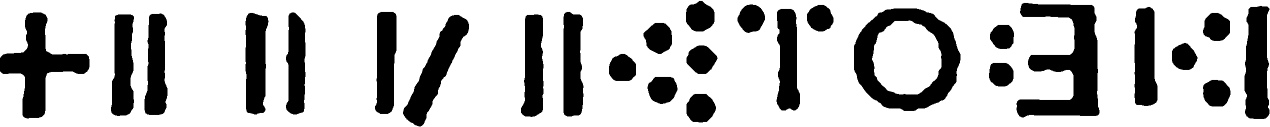
\includegraphics{img/edensymbols.png} \par}
{\slash} Soldiers, helmets cocked down, legs spread, trampling, muscles drawn back, over new-born
babes swaddled in scarlet, violet shawls : babies falling from arms of women huddled on floors of
G.M.C. trucks ; driver's free hand pushing back goat thrown forward into cab {\semislash} Ferkous
pass, RIMA platoon crossing over track ; soldiers jumping out of trucks ; RIMA squad lying down on
gravel, heads pressed against flint-pitted, thorn-studded tires, stripping off shirts in shadow of
mudguards ; women rocking babies against breasts ; rocking movement stirring up scents sharpened
with bonfire-sweat impregnating rags, hair, flesh : oil, cloves, henna, butter, indigo, black
antimony --- in Ferkous valley, below breakwater heaped with charred cedars, barley, wheat,
bee-hives, tombstones, drinks-stand, school, gaddous, fig-trees, mechtas, stone walls oozing
spattered with brains, orchards blooming, palm-trees, swollen in fire, exploding : flowers, pollen,
buds, grasses, paper, rags spotted with milk, with shit, with blood, fruit-peel, feathers, lifted,
shaken, tossed from flame to flame in wind pulling up fire, from earth ; slumping soldiers
straightening up, sniffing tarpaulin flaps, pressing tear-stained cheeks onto burning rails, rubbing
members against dusty tires ; sucking in cheeks, drooling over painted wood ; truck-squad, down in
dry river bed, cutting rhododendrons, milk from stalks mixing on knife-blades with blood of youths
disembowelled in onyx-quarry against central vein ; soldiers cutting back, pulling up saplings,
digging out roots with studded boots ; others kicking, swinging lopsided : camel-dung, grenades,
eagle-carrion ; RIMA squad clambering into trucks, falling onto women, guns at sides, hardened %
\crpage{2}
members spurring violet rags clasped between women's thighs ; soldier, chest crushing baby sucking
at breast, parting woman's hair pushed over eyes, stroking forehead with fingers covered in powdered
onyx ; orgasm spurting saliva from mouth, dowsing baby's buttered scalp ; retracted member resting
softening on shawls soaking up dye ; wind shaking trucks, sand whipping against axles, sheet-metal
{\semislash} soldiers clambering into trucks : RIMA squad, leaning against tarpaulin pressed down on
necks by driving rain, buttoning up ; eyes shining in darkening shadows, fingers glimmering on
belt-buckles ; goats, sweat of pursuit around bonfires soaking coats, crouching down, licking rags
tied around thighs of women ; silent youth wrapped in sackcloth, propped back against driver's seat,
pissing into blue enamel mug held in mutilated hand : driver, leaning back, stroking youth's
forehead marked with blue cross ; youth kissing palm, wrist rippled with veins, swelling with
alcoholic blood ; half-track caterpillars grinding stones thrown onto track by wind ; soldiers
dozing ; dye-stained members curled against thighs, dripping drops of jissom ; driver of truck
crowded with males, animals, bundles, spitting black saliva, wasp-sting swelling cheek, swollen
half-closing eye, pockets crammed with black grapes : tanned head of old man, reddening under white
hairs, shaking against sheet-metal, under gear-stick : with hobnail boots, driver, black saliva
drying on chin, crushing, pulling immaculate locks from occiput, against metal beaten, from below,
by cracked stones kicked back {\semislash} at camp, soldier \colsaid{dogs! wash out my trucks}
{\semislash} females hanging out babies' rags on bushes {\semislash} males setting up tents beside
rubbish ditch : sludge of rotting meat, vomit, glimmering, rosy, under lifeless reeds bending ;
soldiers pushing back, with butts of rifles, women laying babies down in tents ; kicking, punching
haunches of males bent over unrolled tarpaulins ; RIMA squad pushing into den hollowed out under
platform of camp in onyx vein ; faces heated, arms, legs swinging, bottles thrown against walls :
glass splinters falling back into darkened circle pricking, sticking to hardened members shaken out
of dungarees ; beer, wine --- cut with bromide %
\crpage{3}
--- splashing over shoulders, bare breasts of waiter ; RIMA squad rolling, vomiting in corners ;
waiter, greasy shorts slipping down loins, barefoot, tattooed, on ankle, with woman's breast,
trampling on floor-cloth ; edging around counter, pushing cloth alongside lips of vomiting soldiers
{\semislash} two males tying up animals behind tents ; children, arses caked with crusts of dung,
sitting on grass eroded by salt, panting, foreheads covered with dust, heads leaning lifeless on
shoulders, eyes, violet-hued, watching erection of tents ; soldier with curly brown hair, mouth
crammed with black meat swelling pock-marked cheeks, squatting down, soiled member bouncing inside
pants, beside small girl, stroking neck, hand moving down under rags covering throat, groping around
breasts, under armpits : girl's eyes closing, head touching soldier's wrist smeared with grape-juice
; grey drool of hunger running from girl's mouth onto cheek, wetting soldier's fist {\semislash}
gust of wind lifting up, over mounds of excrement, pages of comics torn out by hands of soldiers
crouched over ditches, forcing out tense, burning shit after forays of rape : papers sticking to
fronds of date-palms, stench of defecated grape-juice washing over lieutenant's zerriba :
lieutenant, crouching, naked, in tub of lukewarm water streaked with rays filtered through lattice,
whistling, medallion balanced on tip of tongue, neck-chain held on mounds of swollen cheeks,
purplish glans touching grape-tinted foam, farts bubbling at sides of bronze tub, forcing rhythm of
whistling {\semislash} soldiers --- on mainland : dance-hall bouncers {\dashcom} in fading light,
prowling around tents, untying thongs, crawling on sand, tent-flaps rubbing over backs riddled with
scabies ; males, females, nerves phosphorescent, huddling together around candles, youths, ears
buried, chewing raw semolina straight from sacks ; children pulling aside, with pinched lips,
clenched teeth, rags covering, containing breasts of women, licking half-chewed flour from lips of
youths ; soldiers, tugging at girls' naked legs ; father grabbing candle ; curly-haired soldier,
rolling black meat in vermilion mouth, unsheathing dagger : soldier's hand, quick, covering vulva
buried under scarlet rags, grabbing, pinching ; soldier pulling thigh, drawing sleeping girl %
\crpage{4}
closer : girl sliding over sand towards tent-flaps ; two soldiers, one scalped on temple by eagle's
beak after rape over crowded nest, other sweating gall, dungarees rolled up over shins flecked with
salt, holding down, tying up father throwing lighted candle at soldiers' hair ; curly-haired soldier
gathering girl in arms : girl sleeping, purring, hand spread open over forehead, rocked in rhythmic
trot ; veiled moon casting greenish glow over bared thighs ; ichneumons, sbots, sphex hovering over
soldier's member : soldier stepping over kitchen cesspool ; soldier sprinting over soiled straw,
alongside kennel ; panting, gurgling --- prelude to rape {\dashcom} sweat oozing on bare chest,
waking girl : girl gazing, into soldier's mouth panting open, at threads of meat caught in canines,
lumps held back in cheeks ; soldier standing girl up, squashed against wire fence of kennel,
squeezing, kissing mouth, cavities of ears susurrating with bloody cerumen ; soldier's hand
unbuttoning dungarees, pulling out member ; girl sucking up meat held back in soldier's cheeks,
chewing, eyes closed, hands spread out on fence ; soldier, aroused by movement of muscles from cheek
to belly, bare-headed, straw-dust disturbed rising around legs, injecting girl with clear, hot
jissom ; dogs, woken by wire fence creaking, springing from kennels, chains gleaming, dragging in
excrement ; soldier nibbling at girl's gums, teeth pulling at threads of meat, girl's teeth covered,
defended by tongue ; dogs howling, chains ringing on tarmac, paws grinding into hardened excrement ;
soldier's knees gripping small waist : second orgasm dowsing girl's shoulders ; girl keeping hands
clasped against soldier's sweaty loins ; fence collapsing ; soldier folding, covering girl's body ;
nails scraping earth ; soldier's breath against girl's cheek sucking in, blowing out straw-dust ;
girl shifting belly under grinding muscles of abdomen ; blinding --- nails, spit --- soldier's eyes
; soldier's secreting balls lying, cooling, on girl's thigh ; below palm-trees, RIMA squad dragging
woman pulled unconscious from tent : blond soldier, forehead glowering, tears bathing eye-sockets
glazed with charcoal, urine blocking jissom in glans, squeezing woman held in arms ; \said{screw
good ; fuck hard ; watch out for brass}, %
\crpage{5}
hands, lips, stroking, licking woman's contorted face thrown back over blond soldier's arm ---
oil-smudged, wine-stained {\semislash} small girl, covered, coated with straw-dust --- except on
lips, vulva blocked strangulating soldier's member --- whining, sniffing back bloody mucus into
nasal cavities {\semitwoslash} woman's head hitting scarified trunk : initials, school-sums, hearts
pierced with arrows, of sterile palm-tree ; soldiers, unbuttoned, sugared fists squeezing swollen
members, jostling between woman's legs held apart by two fellows, tension of plexus discharged,
members drooping against thighs, hugged by camouflage-dungarees {\semislash} inside tent, soldiers
sitting on father's stomach, arms, chest, rubbing blackened hair with palm of hands, farting :
candle, stuck into mouth of male swooning, hissing between cracked lips {\semislash} watchtower
overlooking charred palm-grove ; Peuhl sentry, yellow iris sliding into bluish eyeball, sweat
soaking frizzy hair, turning spotlight : beam beating onto sweating flesh of soldiers arched over
woman ; sentry grinding member in fist, turning spotlight : beam crossing dried river bed, catching
vibration, bathed by zephyr, of dusty rhododendrons : pack of jackals tearing at donkey-carcass
filled with putrid liquid --- flanks swinging swollen ; sentry spinning projector on chassis, beam
burning into nipples palpitating pubescent, sprinkled with sugar under drill of dungarees encrusted
with dirt : sweat oozing through tangled tufts ; sentry's throat, beam melting blood, pus, in
razor-cuts ; member forcing starched crotch, pushing out of pants, spreading, arched, under tight
cloth ; sentry, fist spinning projector towards stratosphere, moaning, yawning, rubbing thighs, seam
of dungarees cutting into buttocks, against sheet-metal casing chassis ; soldiers drawing back from
woman wrapped around tree-trunk ; ants, mosquitos gathering seed, jissom forced back out around
exposed vulva, rag --- orange flowers, on violet --- sticking to groin ; soldiers walking, thighs
opened, heels lightened, saliva drying on chins ; tucking away members, buckling belts, wiping
gnarled hands at sides, fingers coated with antimony from woman's hair ; farting ; leaning back
against ladder of watchtower, feet nestling in urine-sodden sand, lighting cigarettes %
\crpage{6}
taken from pockets sticky with jissom, shifting haunches : glans, detached from cotton inside pants,
discharging last drops of jissom ; farts rippling from sweating arses ; sentry squatting, arse hairs
caked with faeces pulling apart, buttocks spreading, pressing nostrils over holes in floor ; scent
of jissom wafting up from soldiers' open shirts, mixed with whiffs of toasted tobacco rising from
lips, from fingers smeared with seed ; at changing of guard, sentry running from tower, hardened
glans pinched in elastic of pants, towards palm-grove behind barbed wire, dragging woman, pulling
feet, beyond tree, into salt-marsh slick, lying over body --- breathing stopped --- spreading
bruised lips of vulva, pushing in member retracting on contact with cooling flesh, kissing woman's
shriveled lips, eyes, soldiers' saliva, spat over iris, drying ; woman's vulva closing around
member, squeezing, crushing ; Peuhl, cold sweat oozing from pores, coating hairs, standing up,
pulling fingers out of woman's wilted locks --- sweat drying in tufts, lice, fleas jumping out ;
flies, ichneumons diving in, heavy with black powder from charred fringes of male palms, digging
down to greenish skin of scalp {\dashcom} carrying fingers to member, squeezing base, pulling at
hairs caught in vulva ; secreting balls clasped in free hand, white sweat seeping : mosquitos, ants
stuck in foam, between sentry's fingers ; breathing, sentry choked by salty stench ; standing up,
lifting woman's hips against belly, stepping forward, legs spread, staggering, weight of woman
pulling down on member, stretching skin over vertebrae of sentry's neck, over atlas, axis, sternum ;
on platform of dry sand, at edge of palm grove, sentry stopping : flies, mosquitos crawling under
cap, in knot of hair on occiput ; woman's legs stiffening, beating against sentry's shins ; sentry
kneeling, sprawling, woman's legs unfolded, varicose veins shrivelling against sand, panting over
cold belly, groin muscles, tissues of member straining ; fist striking around vulva, fingers pulling
on lips, digging, under folds, into stiffened muscles ; Peuhl unsheathing dagger at hips, tracing
with point of blade --- bent : youths gutted against onyx wall --- semicircle around vulva, plunging
blade into mute flesh, tearing, %
\crpage{7}
stripping, slicing muscles, nerves running from vulva into flaccid sheath covering strangulated
member ; member hardened on contact with disturbed muscles, springing out, capped with bloody flesh
; Peuhl gathering, stroking, wiping member on flap of sweaty shirt ; standing up, leaning back
against trunk, picking up rifle from salty platform --- sand, crackling, flying up into face
{\dashcom} coming back to woman, rifle-butt striking face, breasts, --- member recoiling red,
bruised, deformed, against sentry's thigh ; crouching, head turned back, seizing woman under
reddened armpits : sweaty hand slipping on cold flesh ; legs spattered with blood from mangled vulva
dragging on debris of bones ; Peuhl kicking dislocated corpse into hole dug under barbed wire by
jackals, onto bed of carrion, excrement ejected in scramble for spoils ; sphex, sbots, blown up in
draught, assailing --- antennae, stings buzzing --- penis, eyes, nose, lips ; Peuhl burying head in
shirt, stung by wasp beneath right nipple, dung-fly drinking seed caught in hollow of exposed navel
: brisk movement of torso squashing fly in sweat between two folds of flesh ; buzzing, discharging
into sweat, climbing up along fold of flesh toward hip ; Peuhl running, member smarting, hands open
outstretched ; at first-aid post, two bare-chested soldiers groaning, retching, cheek to cheek ;
sprawled under sink, shins bathed pink slapping in vomit, forelocks trailing in gluey mash reeking
of wine ; cadet, squatting, needle jabbing soldiers' bared buttocks : two orderlies holding soldiers
down on tiles ; Peuhl sitting on bench, head thrown back onto shoulder, shaking, skin mottled, teeth
chattering ; penis, blood drying, protruding from fly ; nipple swelling ; cadet, member sprouting,
pushing at fly stained with iodine, standing up, eyes dazzled, level with rounded swelling of
cheeks, fixed on fold, stretched by erection, forming beneath belt-buckle ; two orderlies lifting
up, carrying soldiers to stretchers arranged outside, beside wall of hut, on trestles ; Peuhl stung
on breast, whining, bloody saliva drooling from dried lips, two threads dripping onto chin ; cadet
tearing off Peuhl's shirt, shirt thrown down at feet ; handkerchief in hand, thumb stroking, forcing
Peuhl's lips, teeth : %
\crpage{8}
cadet's member stirring in pants {\thd} \said{{\thd}farting herdsman, dozing, loins stiffened
from thrusting, pumping{\td} slender, running through drinn{\td} pimply mouth{\td}, hot bath,
insecticide, tooth-comb never drawing out perfume of wool, of milk{\td} paste, potash, gonacrine on
your lips, taste of venom sucked{\td} no encrusted dung of buggery on glans hardened by quivering
tension of loins, bitter sweat of beasts squatting in salt{\thd}}{\td} : Peuhl kissing cadet's
fingernails through muslin, nostrils detecting crease, whiff of dried jissom ; cadet dropping
handkerchief, stroking Peuhl's bare shoulder, gathering, rolling member in palm of hand, groping
inside pants, pulling, pressing testicles against folds of cloth ; Peuhl, flanks strained
stiffening, spreading thighs ; standing up, pressing thighs against sink, surrendering, into fingers
of cadet, hardened member : squeezed against porcelain, plunged purplish into bowl of oxygenated
water ; Peuhl stepping outside hut : nest of larks hissing, hooked under palm-awning ; stroking
nest, larks springing up, shitting over wrist ; squatting down, stretching out on straw kept for
tortured prisoners, dozing, buttocks pulled apart by stiffened seam of dungarees ; lips, wet with
spittle expelled by pulsating cheeks --- knees, hams, forehead trembling {\dashcom} touching
blood-spots on pillow{\thd} \said{{\thd}drinking rebel's blood, drinking against tortured lips,
tortured shins, holding blood in mouth, running through fields of blackcurrants blazing, flooded
with venom, wrist chafed by sickle-charm tied to chain, running to meadow with fishes leaping,
outside slave-camp ; over hill, spitting blood into onyx basin ; other slaves, scalps caked with
dung, forehead to forehead, spitting other blood : golden, blue, black ; wind spraying blood over
exposed loins, clouds of excrement shadowing top of hill : under overhanging rock, soldiers blowing
onto bonfire of branches built around mouth of dead woman, blowing in measured breaths, squatting,
tall twisted locks sweeping over woman's breasts ; chest rubbing on fleece over vulva, skylark
caught in tangled hairs ; lark singing, chest pressing against body of woman, tears springing from
eyes ; hot blood trickling from ears ; excremental rain splashing over rock ; blood, in %
\crpage{9}
basin, burning, boiling ; young rebel, bare feet daubed with onyx powder, lips with flour, rising
from earth, leaning over basin, immersed head, fists ; raising head dripping with blood, hurling
raucous cry towards hills, bushes moving : lions springing out ; lions lying at rebel's feet,
licking behind knees ; young rebel, scooping blood mixed with excrement in cupped hands, showering
lions' manes ; around camp, women slumping against fences, soldiers' members straining towards
mothers, brought from mainland, for Slave-Feast ; carrying Mother into bamboo hut, laying down on
bed of poisoned straw : head, shoulders buried beneath Mother's dress, eating fruits, antelope
fritters over hardened vulva : Mother sleeping, tired by journey in cargo hold, tipper-trucks ;
escaping at dawn, slipping from under my body ; caught by soldiers under tower --- me watching,
ejaculating --- pushed back onto sand by goading knees, wasp hovering at right breast, over lips of
soldiers sucking at teat{\thd}}{\td} {\semislash} pressed against kennel fencing, soldier rolling,
covering girl ; cadet squatting down, lifting up soldier, gripping loins : member slipping out,
soldier standing up, running off ; cadet blowing off straw gathered on small contracted body,
lifting girl up in arms ; body dilating under breath, vapours, juices of cadet --- hugging girl,
chewing ration-biscuit, girl kissing cadet's lips, tongue collecting crumbs stuck along gums ; cadet
laying girl on bed in sick-bay, bathing mangled vulva ; feverish, cheek bloated with vomit, stepping
back outside, switching on lights over latrines --- soldiers working on group of women {\dashcom}
lifting up fainting soldiers, stroking forehead of women sprawled on ground, separating native
mercenaries coupling, pulling apart couples stuck firm by compression of plexus ; returning, washing
under running water : hands, arms, neck, smeared with jissom, with seed ; cadet, vomit expelled,
carrying out girl swaddled in surgical smock, opening tents, in turn, tipping girl's face back into
candlelight ; opening tent with two soldiers holding male, filled with sand heated through by
movement of limbs clutching, sweating, radiance of muscular contractions ; cadet shoving soldiers
aside --- standing, penis retracting beneath cotton %
\crpage{10}
{\dashcom} placing girl at feet of female, lighting candle taken from mouth of male, pushing
unbuttoned soldiers towards opening of tent --- at corners of lips of female, drop of jissom
shimmering {\semitrislash} in bunk-rooms, bamboo waving in dawn wind, insomniac soldiers, naked,
sitting cross-legged on bedding, picking at stained members ; suspect youth, caught reading
shit-smeared cowboy comic in front of tent, thrown bare-chested into command-post : cheek, chest,
belly marked by hand-prints, in blood ; sergeant capping suspect's bloodstained head with empty
coffee-pan ; sugar sticking to hair, mixing with blood, filling ears ; soldier on fatigue-duty,
frayed dungarees stretched over arched buttocks, bringing back bludgeon, smeared with excrement,
from toilet ; hitting shoulder of suspect : three blows, jaw : seven, with end of stick coated with
creosote, pressing stick into suspect's fist ; driver taking spanner, crank, from truck ; spanner
forcing open suspect's clenched jaw, driver unbuttoning dungarees, pissing between torn lips,
pulling up suspect with three spanner strokes at throat, pushing crank through tear in dungarees,
between buttocks ; other soldiers aroused, rising from mattresses, grasping, turning crank in
suspect's arse ; suspect, head falling back, wet with spittle, onto shoulder, crown touching
tormentor's swollen crotch, lips spitting back excremental saliva, clenching teeth onto spanner ;
tip of crank forced into loins ; pulled out, bloody, by driver, thrown outside command-post, wiped
clean on sandbags around perimeter ; suspect youth swooning, collapsing on mattress, unbuttoned by
soldiers --- spitting, farting ; with barrel of rifle, soldiers lifting up, pressing penis back onto
belly : sergeant's studded boot squashing flesh ; red-haired soldier, hollow eyes, glans sprouting
--- caught violet between two gaping buttons {\dashcom} leaning over, grabbing, tying testicles of
suspect in soiled rag pulled from under bedding ; fingers stroking small neck formed at root of
compressed member, junction of knotted membranes {\semitwoslash} suspect revived in empty guard-room,
cadet kneeling, untying rag ; sentry, mouth rosy in dawn fire, walking on terrace, legs bowed, fist
buried inside pants ; leaning back against palm-trunk propped up by %
\crpage{11}
brownstone balustrade around terrace ; stiffening legs, pulling out member ; rifle, loaders,
clicking at loins, masturbating, helmet pushed back over neck, jugular vein outlined in creases of
throat, tongue protruding from mouth ; two children squatting, defecating against barbed wire ;
soldier levelling projector-beam towards point on horizon --- dawn fire looming ; woman from tents,
breasts swinging in patched silk, flowery silk sticking at pubis, haunches slumped against barbed
wire, fingers scraping shit between children's buttocks, wiping fingers in sand ; red fist on white
arm, slipping between wire-mesh, touching sliver of ration-bread poking from sand, intact ;
soldier's rifle slipping from shoulder, barrel knocking against projector chassis ; one breast
springing out of silk ; member forcing soldier's fingers ; thumb of other hand, loosened by
accelerating movement of masturbation shaking, contracting shoulder, milking-arm, jerking, touching
trigger ; woman, throat riddled with bullets, collapsing, head, hair fading dead, rolling onto
shit-smeared wires ; jissom spurting, splashing boots, sheet-metal ; between breasts, fresh blood
bubbling in globular clot ; soldier linking index-finger to trigger-thumb, squeezing member at root,
pressing jissom up towards violaceous glans, catching drops in fingers : tepid, carried to lips ;
children, faces, bellies, swollen behind tears, heads muffled in heated rags, pressed against pubic
curls, sleeping, sobbing, thin bodies shaking, waking, crying --- entrails cooling, {\twoslash}
Wazzag, wiping mouth smeared with egg, mint, jissom, pulling damp leg from under whore-master's
belly : master asleep at right side of whore ; sheet clinging to loins, Wazzag rising from bed ;
naked, going down stairs ; ear-rings tinkling : lowering forehead --- powdered jissom held in
wrinkles --- under lintel closing off counter ; red-haired boy lying on belly in box-room among
floor-cloths, buckets, brushes, pressing forehead, knees, against concrete, replenishing jissom ;
goose stretched out beside boy, beak burrowing under armpit ; Wazzag lifting up goose holding neck,
hand rubbing boy's nipple ; pulling bird out of box-room{\td} \said{just grabbing gobbler,
Khamssieh, time for lame-duck to get good goosing{\td}} ; %
\crpage{12}
goose squawking, Khamssieh rolling over onto back ; mottled member bouncing out between thighs,
springing up erect ; tongue lolling over lips ; clot of jissom trembling in nostril, blown onto
fingers, Khamssieh rolling onto side, burying clot between buttocks ; jumble of rags piled against
back wall, boy's fingers groping towards drain linking box-room of boys' brothel with tile floor of
women's : blood mixed with jissom wetting fingers ; Wazzag throwing goose into first latrine along
passage leading to garden ; boy huddled in corner, heavy torso squeezed into white singlet torn at
nipples, rest of body naked, right foot in bracelet : foot slipping on edge of toilet-hole, leg held
back, hands crossed under knee ; penis, uncircumcised, dragging on soiled concrete ; Wazzag holding
back goose by wings ; boy cowering in corner ; movement of long eyelashes startling goose, beak
opening ; Wazzag loosening grip, goose springing at boy's throbbing neck ; boy, pulling up body
along piping, grabbing goose's neck : penis hardening, brushed by spur-claw, by plumage ; boy
burying goose's neck between thighs ; Wazzag stepping out into garden, leverets jumping in cages,
Wazzag offering penis, leverets nibbling ; leaning back against tamarisk --- trunk tied with
club-foot's cast-off clothes {\dashcom} tying foliage torn from tree around arms, hands, heel, spearing
greenest sprig with violet tip of glans, hardened by leverets' tiny teeth ; Wazzag jumping onto
terrace of women's brothel --- secreting balls, encrusted with dirt, slapping under buttocks ; in
alley, worker-youths, date-pickers, mechanics, lubricators, quarrelling over Khamssieh leaning
against door-post, workers' hands reaching for dark tangle planted in wide milky body ; Wazzag
squatting beside trap-door : platoon of soldiers back from South unbuttoned by girl-whores ; one
soldier approaching : before seeing head, just catching curve of member projecting from dungarees,
Wazzag : {\td}\said{Rico, my flower{\td}} : soldier stepping onto terrace, away from
girl-whores, scratching dirt between toes with moistened thumb, Wazzag kneeling, fresh scent of
insect-seed rising from leafy limbs, flicking dust from mop of hair dirtied in fatigue-parties,
bivouacs, soldier hugging Wazzag between two rows of %
\crpage{13}
sheets hung out under reddening fire ; below. in women's brothel, noisy soldier with shaved head,
bluish at temples, diving at black girl-whore --- thrown back against pink wooden stairs, crossing
heels around soldier's ankles, over boots {\dashcol} English box of love-powder, swapped in South
for handful of sugar, slipping from soldier's pocket, whore grabbing, opening box, sniffing powder ;
black whore, loins battered, blowing white powder between soldier's honeyed teeth ; soldier spitting
back powder onto whore's lips ; soldiers pressing fists between women's breasts, pulling back,
licking sweat soaked up under thin cloth ; whores unbuttoning, one by one, soldiers thrown back over
thighs ; soldiers' members rising at contact of fingers, palms, retracting under bracelets, rings ;
pubic sweat clouding coral, silver {\semislash} shoulders hunched, Khamssieh tucking penis between
thighs ; workers, pressed against moist body of boy-whore, caressing, slipping fingers under arched
fundament, searching for trapped penis ; Khamssieh, arms raised, crossed behind neck, laughter
exploding ; grease-smeared hand groping under buttocks ; laughter shaking boy's shoulder touching
cheek tipped sideways{\td} \said{{\td}first round for you, darling, come dip into soup you shot up my
nose this morning ; kept my meat fresh for you{\td}} ; lubricator, holding rump of whore with
one hand, other unbuttoning overalls, member springing out, catching polished membrane of
Khamssieh's secreting balls, pushed back towards arse by pressure of thighs over penis ; member
quivering, hardening, pubic hairs opening out ; Khamssieh kissing mouth of black child hanging onto
shoulders of date-picker, lips smacking ; kissing cheeks, scarified throat, chest heaving under
half-open jacket ; child's hand holding pomegranate ; trace of oil gleaming mauve suspended in
woolly hair ; Khamssieh sliding hand under date-picker's armpit, groping at child's thigh, hand
enveloping member, secreting balls, through tight denim ; saliva filling child's mouth ; Khamssieh
kissing child, child pushing saliva between teeth of whore : lubricator, flaps of unbuttoned denim
jacket covering, brushing over Khamssieh's hips in movement of erection, buggering Khamssieh, sweaty
chest sticking to boy's back {\slashsemi} flight of sand-%
\crpage{14}
larks swooping into alley, dancing over flock of sheep marked on forehead, ochre, red ; shepherds,
poxy, resting --- animals shitting {\dashcom} slow watery gaze fixed on bars of women's brothel :
free whores smiling at shepherds, foam shining on swollen lips, uncovering breasts ; shepherds'
fists slipping between bars ; members stirring between thighs, rags pulling apart ; bottom of
stairs, black whore, lips smeared with love-powder moistened on lips of soldier, dragging ---
holding feet --- soldier unbuttoned, penis erect, to threshold of saloon ; jissom, spread over
testicles squashed under soldier's buttocks, glistening in cracks of tiling, whore pulling soldier
over floor ; two soldiers, standing, naked, on one side, other side, of belly of girl-whore
stretched out at feet, throwing mixed threads of jissom onto pubic fleece, each soldier grabbing
other's throat with sticky fingers, spitting in other's eyes ; members heating, opening out ;
soldiers' thighs pushing forward, bristling hairs mingling, two members standing together, held in
bundle ; chins covered with foam, each gnawing at other's teeth, pulling closer, hands of one joined
pressing, lifting buttocks of other ; lips stuck together, nostrils sniffing up foam spreading back
over jaws ; each stroking other under penis{\td} \said{{\td}fucking dick{\thd}}, grabbing
testicles ; pubic fleece tangling together ; girl-whore standing up, pulling soldiers apart,
soldiers squeezing whore, moving across, hurried, in small steps, to wall ; orgasm : jissom pushed
from vulva, from arse, gluing bristly hairs onto soldiers' thighs ; girl-whore, shaved head marked
with scabies, whispering, pressed against bars ; shepherds stroking bare breasts squashed against
dusty grid, pulling nipples between bars ; lifting rags, uncovering, shaking pock-marked members,
clacking infected tongues ; whore moving lips, two fingers making gesture of masturbation ; mouth :
lips, teeth, jaw, movement of sucking ; shepherds pulling small eggs from under rags, whore closing
wooden shutter behind grid ; head-shepherd, blowing into flute --- rising urges throbbing in throat,
breath shaking in pipe {\dashcom} leading flock towards outer ring-road ; rear shepherds unhooking
fingers from grid, picking up sticks, striking, tucking members into rags, %
\crpage{15}
shaking secreting balls assailed by flies ; top of street, old men, children, sleeping on steps of
slaughterhouse strewn with skins, with bloody fleece ; black girl-whore pulling soldier with bluish
temples up to foot of cradle ; soldier, hardened member swinging in half-light, licking pink wooden
wheel of cradle ; whore squatting down, stretching out over moaning soldier, beating member
alongside half-open vagina ; jissom overflowing ; whore squashing soldier's softening penis into
sticky mass of balls, membranes, curly hairs, kneading, pressing down, pulling back, pushing penis
up towards belly : soldier nodding asleep under heavy throbbing of veins shining on prismatic scalp
; flock crossing through souk set up beside ring-road ; slim, laughing, naked under light robes,
high blue hair sprouting from veils braided behind necks, nomads unrolling pieces of yellow oilskin
cut from insulation of underground pipes beneath nuclear station --- sold as tent-sheets, to negroes
; sheep trampling over oilskins ; nomad youth, standing up --- ear-rings shaken, tinkling,
glimmering {\dashcom} leaping in front of head-shepherd, member spurring, wetting blue robe ; two
boys kissing on mouth ; breath of nomad washing over shepherd's ear : {\td} \said{{\td}akli{\td} my
lamb{\td} come suck{\td}} ; shepherd, kneeling, kissing nomad's navel, sliding flute under string
tied around knee ; rear shepherds moving to front of flock ; nomad pushing milk-brother through
covered market, into back-room of barber-dentist ; sitting down in shaky revolving chair, spreading
long legs under stretched robe ; shepherd kneeling in floor strewn with teeth, locks of hair,
rolling up nomad's robe ; peasant youth, mouth spurting blood, crying out : bloody turban wrapping
youth's red hair, one tuft, beaded with sweat, sticking out of cloth over skull, bushy, flaxen,
caked with scabs --- from pubis, armpit ; thighs of youth, hugged in jeans, twitching ; white seam
of fly bulging at crotch ; pubic sweat seeping through denim, dampening leatherette cushion on chair
; peasant youth's dilated nostrils drawing in, blowing out blood mixed with enamel dust ; shepherd
squeezing nomad's thin thighs : scent of camel-dung rising from penis lifted up in shepherd's
chapped hand ; shepherd placing %
\crpage{16}
lips on dry pubic fleece : line of sweat glistening along fold of thigh, shepherd grabbing encrusted
balls in one hand, other masturbating short member --- tiny veins, stretched by erection, simmering
against cheek ; nomad tensing legs ; jissom spurting, shepherd rolling back tongue into throat ;
jissom, heavy, fresh, filling mouth ; clots chewed between teeth --- decayed by excess of oil, of
carrion ; nomad tensing legs, sand held in hairs running down hardened calves ; second orgasm
hollowing belly, narrow bust, relaxing muscles of legs ; shepherd's fingers pressing cheeks filled
with thinner, warmer jissom ; nomad, fingers spread, pushing away head of shepherd diving back
between thighs ; standing up, pushing aside shepherd still kneeling --- head bent down, eyes fixed
on ground, lips closed over jissom caught between teeth ; nomad, with tip of naked foot, pulling at
rags held between shepherd's buttocks ; shepherd standing, pulling up soiled rags --- detached from
caked excrement --- over hips, spreading legs, buttocks held open with both hands ; arching top of
body, jamming head against burst bundle of rotting linen ; nomad's hands crossed under shepherd's
belly, shepherd's palms, fingers, rubbing nomad's thighs, nomad pressing member into shepherd's
arse, shit-caked --- rags torn back revealing fresher layer of excrement --- hairy ; top of
shepherd's body bending, weighed down --- shepherd inverted, dizzy, relaxing pressure of hands,
buttocks gripping tighter onto nomad's member {\dashsemi} nomad holding back body articulated around
base of member, crossed fingers squeezing shepherd's belly ; orgasm spent, bending torso over
shepherd's back, saliva running from lips into shepherd's ear \colsaid{{\td}my lamb, one thousand
dinars your price, naked {\thd} my father dead in Tamesna{\tdcom} {\td}purple body buried in sack
of salt{\td}} {\semislash} flock stopping at edge of cliff ; mist rising from swelling wadi,
covering negro village ; sheep butting naked babies propped against trellis-fences, wallowing in
fech-fech ; children, tickled by rubbing of wool, lying under bellies of sheep ; elbows pressing
down, puffing out stomachs, rubbing against animals' nipples ; shepherds squatting at bottom of
ravine opening into roaring wadi, masturbating, changing %
\crpage{17}
position on pebbles --- contraction of nerves, muscles, bringing kneecaps near breaking ; female
sheep lifting penis of child leaning back against rusty metal urinal --- dragged from town centre
during night of riots, by youths with knobbled skulls {\dashcom} licking fresh excrement splattered
over child's buttocks ; returning to lamb, licking under tail ; turning back, burying muzzle between
legs of child, child spreading thighs, caressing cold eyes of ewe ; in communal gardens, women
scything barley, wheat ; wrists, arms marked with scabs, violet scars : viper-bites, sickle-cuts,
djerid-wounds ; child, wearing blue-spangled dress, hanging onto mother's robes ; mother lifting
head, forehead catching clear beam of reddening fire filtered through palm-trees ; dazzled, bending
back down, throwing scythe aside, into uncut clump ; hook catching child hidden in clump ; through
torn cloth, line of blood forming across swollen belly from right hip to left groin ; girl falling
onto bed of wheat, forehead, lips fading white, scythe stuck into flesh ; in village, children
tormenting live toads --- shitting in hands --- caught in pink sand-marsh ; impaling toads, swollen,
on trellis-fences : impaled through ribs, falling, flesh giving way, down along spikes of trellis in
gardens --- children, drowsy, laid down, enclosed, in gardens until nightfall with lambs, kids :
woken on contact with cool of sand, falling back, rocked asleep by bells of lambs, kids lapping
tepid brackish water of irrigation ditches, hidden beneath barley ; shepherds, shivering, standing
up ; rags trailing in jissom, sticking to thighs ; globules glimmering on black shingle ; shepherds
mounting favoured sheep ; wiping, on fleece, articulation of thighs, edge of arse, covered in sweat
from movement of masturbation ; touching embalmed wool, members, softened, hardening, burrowing,
gleaming violet, into dirty fleece ; women, gathered around wounded girl, heads turning back ;
shepherds, testicles squashed under buttocks against protruding bones of sheep, bare feet stuck into
warm sand, tongues lolling over chins, panting, yelping ; rutting dogs rolling in wheat, snapping at
dresses of women ; rolling in sand, snapping at members of shepherds ; russet dog licking girl's
wound, running towards shepherds, rubbing %
\crpage{18}
against leg of shepherd with biggest member, pushing burning tongue between thighs ; tongue wrapping
member ; dog's breath bathing shepherd's belly, foam running down thigh ; shepherd, stiffening legs
against flanks of sheep --- dog surprised by muscles cracking, jumping aside : shepherd's lips
puckered, moist with foam, arse-hairs rippled by light fart, animal returning, tongue catching
member {\dashcom} heaving, fingers hooked around ears of sheep ; jissom spurting : held by dog on
tongue curled back, carried into clump of wheat, laid at women's feet {\semislash} in saloon, baby,
lifted out of cradle, crawling along trace of jissom trailing between legs of soldier with bluish
temples, trapped under thigh of black girl-whore : flap of blue woollen rompers dragging in clear
jissom ; young whore sitting cross-legged on tiles, taking baby into lap : combing, with small blue
nylon brush, pubic fleece of blond soldier marked on groin with beauty-spot ; soldier's back
rippling spotted with green paint, transferred onto skin --- soldier masturbated first by
whore-mistress, body stiffened against green wall of orgy-room moistened with sweat, pressing back
at shoulders, buttocks, calves, neck bending, head congested purple ; soldier standing, hand on
shoulder of whore, dungarees around ankles, nipples smeared with honey under gaping shirt, eyes held
veiled in measured beating of masturbation, fixed on bundle of machine-guns propped up in corner
beside drain --- through hole, muted murmur from boys' brothel {\dashcom} sighing : brush pulling,
disentangling knots of curly hair ; fist of whore gripping reddened member sticking to fingers,
scattering quick kisses over soldier's belly : knots of hair torn out --- follicles rotting in
polluted cuticle{\comdash} caught by whore in powder-box at feet ; lifting baby towards soldier,
baby's lips touching violaceous tip of penis, soldier's forehead glowering purple ; below stairs ---
framework pegged to box-room wall, packed with stocks of jam, eggs {\dashcom} two soldiers ---
girl-whore squeezed against wall, abandoned --- squatting down, lifting cellophane, sucking up jam
from one jar ; tongues touching in jelly{\td} \colsaid{{\td} Khamssieh, tongue never fit in
jar{\thd}} ; boy's raucous laugh resounding along partition, broken by smack of %
\crpage{19} % TODO hamac -> hammock?
wet dishcloth on bare flesh{\td} \said{{\td} silence, arsehole, making me droop!} ; blond soldier
drawing head of girl-whore towards crotch, picking up brush, combing thin hair on temples, eyebrows
sticky with fresh jissom ; right arm of whore{\comdash} left holding member {\dashcom} hugging
soldier's loins ; fingers plunging between buttocks ; soldier's member hardening, forcing whore's
fist, loosening grip ; hand of whore kneading soldier's buttock, fingers palpating membrane of arse,
nails scraping layer of excrement {\thd} \said{embers fading under half-cooked joint, black blood
spurting deep in throat{\thd} cutting tail of gutted jackal, pressing tail between my buttocks,
squatting on rock, ears pricking up in salty wind, rain lashing lips closing over squirting blood
{\td} Rico cutting into animal's muzzle, hollowing, emptying with dagger, burying head inside,
kneeling in mud{\thd} walking towards rock, outcrops of flint catching my member, Rico pushing,
between my spreading buttocks, jackal's bloody muzzle{\td} pulling mask up against my loins, working
lips against my arse{\td} black colic churning in my belly{\td} ejected, filling mouth{\td} Rico
standing up, spitting out excremental stew{\td} crouching back down, browsing on sodden moss,
chewing, staring, me squatting, legs stiffened, rain lashing tensed muscles, pumping member softened
by rain --- at tangled brown hair of my dripping groin{\td} Rico standing, leaping at my streaming
body, knees knocking, Rico's hand smearing jissom spurted onto my thigh{\td} kissing imprint from
webbing of hamac on back of my neck, teeth pulling downy hair of nape, greasy curls over my
ears{\td} knee raised between my thighs{\td} US shorts, thrown down onto moss, holding, under
downpour, folds fixed by constant tension at my crotch{\td} sliding along Rico's half-naked
body{\td} my lips, pressed against moist cloth, following rising jissom in member hugged by
shorts{\td} jissom spurting, my tongue lapping, pushing inside shorts, gathering drops streaked with
thin blood{\td} monkeys whistling in cedars : I walk with Rico, naked, in front of rebels, members
erect, cheeks tipped against shoulders, eyes narrowed, oh rebels, your bellies are light, your
cheeks, daubed with paint{\thd}} {\slash} Peasant sitting on bank of wadi, five teeth intact
chewing %
\crpage{20}
mouse-carrion ; kneeling in mud, sucking up grey water swelling blood-spattered mouth, spitting red
water back into stream, pulling penis from jeans, soaking, rubbing member under water, pressing torn
fingers into folds of flesh{\thd} {\slash} Khamssieh, lubricator's jissom streaming down legs,
leaning back against box-room door, letting workers spit into red hair, pull at member, grasp
testicles, discharge against sides of buttocks, slap cheeks, belly, buttocks, with soiled hands,
force dishcloths between thighs, gag mouth with soaking rags ; worker's member, dry --- jissom held
back surging inside {\dashcom} pushing deep between buttocks, Khamssieh relaxing arse, tilting torso
; hips of worker battering loins of boy-whore ; chapped hand, fingers polished on steel, grabbing,
pulling erect penis from between buttocks, squirting ; workers jostling, hands, jissom-spattered
members rubbing over curve of buttocks, throwing Khamssieh against black child carried on shoulders
of two date-pickers ; three erect members stretching arse, workers pressing in, nipples crushed
against sweaty skin of Khamssieh's back ; stained hands squeezing neck ; black child springing
forward ; jissom squirting from three members bundled together, shaking Khamssieh ; legs of workers
standing at sides quivering along legs of whore ; groans rising from lips, workers pulling out
sticky members ; members, pressed together, springing back hard ; black child struggling, puffing,
spittle oozing out along curve of panting mouth ; touching testicles of workers pressing warm mass
of porous membranes against buttocks, Khamssieh rolling head over shoulder into hot cupped hand of
worker ; worker's hand palpating Khamssieh's earlobe ; fingers delving into eye-socket at moment of
erection ; after orgasm : hand, moist, sliding along whore's cheek, rubbing at creases of throat,
falling back onto surface of buttocks ; phalanges of workers' hands --- pulling out members ---
rolling in slimy folds of Khamssieh's buttocks ; workers drawing back ; two date-pickers dropping
black child ; child diving at Khamssieh ; erect penis of whore pressing against sweaty torso ; arms
squeezing Khamssieh's loins, head pulsating, heating, buried in thighs of whore ; blue spittle
sticking %
\crpage{21}
down strands of Khamssieh's pubic hair ; child's tongue probing between curls, touching infected
cuticle ; lubricator, emerging, buttoned up, from latrine, enveloped in cloud of excremental stench,
rubbing against Khamssieh ; flick of tongue licking whore's lids, end of tongue holding lips
half-open ; whore's member springing back against black child's armpit, lifting shoulder of jacket ;
Khamssieh, chest thrown forward, palpating child's buttocks, sexual cluster squeezed inside jeans ;
child squatting on heels, spreading Khamssieh's legs, kneeling, diving between slimy legs, spinning
on knees ; laughing, short pink tongue licking soft hairs stuck down with jissom, Khamssieh's
testicles dragging on collar of jacket, child standing up, clinging to whore ; Khamssieh, hollowing
vertebrae, bucking coccyx, one hand, slipped under flesh of buttocks pulled up sweating, palpating
boy's belly, unbuttoning jeans, pulling out penis over elastic of pants ; child sucking at hollow of
collar-bone ; hips shuddering against loins of whore ; Khamssieh, with two fingers, pulling back
child's grimy foreskin, sliding two ringed fingers alone hardening shaft ; child's fingers catching
folds of flesh at Khamssieh's waist, legs stiffening against Khamssieh's --- relaxed by movement
separating buttocks ; jissom bubbling in member throbbing against smooth slit of Khamssieh's arse ;
child's body shuddering, Khamssieh's arse closing on glans ; jissom spurting ; taking turns,
exhausted, workers, jissom spent, picking up, from counter, pomegranate brought by black child in
payment for Khamssieh, carrying, licking, crouched in latrine, blood surging in skull, wetting fruit
with foam frothing from lips --- belly forcing ejection of excrement ; child's fresh breath over
shoulders --- in orgasm, child lifting neck --- making Khamssieh shiver, workers' jissom cooling
inside loins ; Khamssieh, quick, spinning around, squeezing sated boy, kneeling, grabbing, pressing
sticky penis, pulling out thread of jissom, carrying filament to lips, standing up, kissing boy's
mouth --- boy's eyelashes beating, moist with cold sweat ; Khamssieh putting softened penis back
into pants, buttoning jeans, taking pomegranate perched on edge of counter, sitting on %
\crpage{21} 
step-ladder, teeth opening pomegranate wet with saliva, burying slimy muzzle inside ; free hand
groping under testicles, untying knotted curls stuck down by stale jissom pulling at skin with
movement of thigh ; member, intact, shining, glimmering prismatic, straining engorged --- workers
laughing, puffing, panting in latrines, dirt on foot-slabs squelching beneath espadrilles under
suspended movement of masturbation, tuft of blue hair shining wet with jissom poking from
half-buttoned jeans of worker emerging, wet spot marking lump under denim filled inside with
softened member swollen by lingering urge {\dashsemi} lubricator, forehead wrapped in soiled turban,
prowling, hands in pockets, jeans tight between thighs ; blue gaze piercing Khamssieh's veiled eyes,
tongue protruding between lips ; belly exposed, inflated, shining with grease, perspiring, grimy
sweat running from navel ; black boy rubbing against Khamssieh's thigh, pulling, drawing leg away
from step-ladder, palpating stiffened limb ; testicles of whore, striking hairy surface of thighs
--- bouncing from one to other {\dashcom} squashed beneath buttocks, sweating onto soiled wood ;
pushed out, spreading over corner of step, in space between legs ; lubricator's hand groping ;
Khamssieh pushing black boy back, bringing balls onto step : seized by lubricator, weighed in hand,
Khamssieh standing up, squeezing loins of lubricator leaning lop-sided, covering --- fingers of left
hand spread --- raised buttock, held up by hardened crease of jeans, right hand palpating other
buttock, relaxed ; Khamssieh kissing lubricator's low wrinkled forehead, roots of dusty hair ;
lubricator shuddering, fist squeezing Khamssieh's balls ; whore, lashes brushing down over top of
rounded cheeks, detaching lubricator's fingers, moving off, loins rubbed from front to back ;
lubricator standing up ; relaxed buttock sliding up thigh of whore ; Khamssieh, lifting penis onto
belly, balls suspended on fold of jeans between buttocks, unbuttoning lubricator, pulling down back
of jeans, back of pants --- held at belly by curve of rigid member {\dashcom} drawing away from
worker : member, released, springing out horizontal, glans scraping over elastic of pants ;
laughing, Khamssieh, fingers hooked over lubricator's %
\crpage{22} 
shoulders, pressing, bending vertebrae, plunging member --- jissom seething --- into shit-caked arse
; pumping : sweaty toes tightening over lubricator's espadrilles ; glans, pressing into arse,
expelling burning jissom ; lubricator standing up, hands thrown behind back delving into Khamssieh's
softened belly ; quick, whore pulling hands aside, stiffening ; jissom oozing between lubricator's
buttocks. skin sticking to top of pants ; Khamssieh pushing half-circumcised penis forward,
discharging runny jissom ; lubricator letting head roll onto shoulder, ear bathed in Khamssieh's
seminal panting ; jissom forced back between lubricator's buttocks dripping into crumpled pants ;
Khamssieh's hand slipping into pouch, pressing sexual cluster into gob of jissom ; lubricator
moaning, tongue licking foam frothing over Khamssieh's thick lips ; flow of jissom, after fourth
orgasm, reaching Khamssieh's foot stuck into lubricator's espadrille {\semislash} club-foot, leg
assailed by excremental worms driven from toilet-hole by cold chilling excrements, coughing ; goose,
aroused by excremental stench, raising neck, squawking, struggling between club-foot's thighs ;
date-picker, crouching in adjacent latrine, hitching up giant body ; clapping hands over top of
partition, thrusting from pelvis, jeans buttoned, hurried, over soiled arse, hanging onto partition,
top of body swinging into darkened latrine : eyes, blinded, adjusting to darkness, discerning body
of club-foot squashed in corner : bracelet ringing right arm shaken, trembling, singlet swelling
over nipples, softened penis stretched dragging in scum of toilet-hole, goose-down fluttering over
damp thighs ; club-foot raising head, neck throbbing, eyes, pale, fixed on date-picker's face ;
saltpetre running through hair ; date-picker's arm reaching out, grabbing club-foot's shoulder,
pulling, lifting boy ; calf tense, pecked by goose, boy springing up, torso sticking, scraping
against partition ; date-picker lifting boy, standing up in second latrine, pulling --- boy hitched
up to midriff over top of panel, hand covering sexual cluster ; date-picker, with one quick
movement, swinging boy over ; rough concrete grazing club-foot's member, tuft from pubic fleece left
sticking to concrete ; wounded penis quivering against date-picker's thigh ; %
\crpage{23} 
boy's foot hovering, suspended over concrete, trampled by date-picker ; boy, thrown off balance,
falling into hugging arms, kissed on mouth ; feeling date-picker's member throbbing, hardening
against his belly : rushing, pulling out of embrace, diving into passage ; date-picker following,
into saloon : boy, standing in corner, singlet pulled down pinched between thighs, club-foot ringed
with bracelet lifted against toe of other foot, panting ; date-picker unbuttoning, pulling member
out of jeans, spinning sideways, hands spread pressing onto nape ; rigid member catching reddening
beams of declining fire, bouncing ; club-foot, relaxing grip of thighs on flap of singlet, diving
forward ; boy's arm, raised defending throat, absorbing shock of body swollen with blood, with
jissom : hand, quick, grabbing, squeezing, holding date-picker's member pressed back against lower
belly ; date-picker's body softening, sinking down ; club-foot kneeling, lifting member to lips,
pressing into mouth ; tongue delving, tip drawn out pointed, into folds, porous membranes, scars,
ritual cuts ; lips vibrating ; quick movement of date-picker dazzled by reddening fire forcing glans
into club-foot's throat ; boy, teeth nibbling tense flesh of penis, choking, coughing : spittle
expelled from consumptive throat of club-foot splashing member of date-picker {\semislash}
{\td}lying on terrace embalmed in foliage of tamarisk fallen from Wazzag's body, robes gleaming
ochre, blue, whore-mistress, legs spread, watching soldier --- spot of wine marking right
eye-socket, spreading onto pock-marked eye-lids --- chuckling, hanging mirror over mud fire-place,
perching glass of hot water on high-chair --- baby undressed, exposed to draughts, taking evening
gruel {\dashcom} shaving cheeks, neck ; soap trickling under shirt opened down to loosened belt ;
whore-mistress licking fingers, raising leg, touching soldier's thigh with tip of toes{\td}
\said{easy, sugarplum.} ; flight of sand-larks invading terrace : reflection trembling in mirror :
females, babies, snuggling into pockets of hanging aprons ; males gathering curls of hair, fleece,
wool fallen from bodies of shepherds, sheep ; soldier shaving around lips, foot of whore-mistress
pressing down on softened member, soldier's mouth pressing against warm %
\crpage{24} 
glass of mirror, kissing sunny reflection of lips ; Rico, Wazzag, fastened together, stepping back,
between sheets, towards edge of terrace ; Wazzag's pubic fleece stroking surface of Rico's buttocks
; Wazzag's chest --- skin stretched down towards pubis {\dashcom} laughing head, crossing top of
mirror, vermilion ; soldier, fist clutching razor, diving at whore-mistress, fingers spread pressing
nipples stuck to cloth ; leaning on woman, spinning around on belly, pressing head between thighs of
whore, into layers of crumpled cloth ; whore-mistress, pulling back flaps of dungarees, seizing,
milking hardened member over lips ; soldier uncovering woman's vulva ; shaving pubic fleece ---
sprouted since full moon {\dashcom} slow, distracted, lips licking pollen held in soiled embroidery
of dress, eye, veiled in orgasm, fixed on Wazzag's raised heel straining, tense ; girl-whores
lifting up soldiers unbuttoned against wall of saloon, sucking up, spitting out last drops of jissom
onto fingers stained with henna, each eating globules from hands of others ; soldiers dozing, heads
weighing on shoulders : blond soldier with shoulders marked green pissing --- interrupting
masturbation --- over knees of whore, whore's free hand --- other hand, splashed with jissom,
pressing sticky member {\dashcom} smeared with excrements reeking of jackal scraped from between
boy's buttocks, panting, from corner of soldier's mouth to ear-lobes, fangs, jowls of jackal
{\semislash} at top of street, on steps of small butcher's shop painted red, children, wrapped tight
in sackcloth, drowning brood of short-eared owls in pool of mixed blood : female, perched on corner
terrace of brothel, screeching --- piercing : children seizing chicks, plaintive : chicks drowning,
waking masturbated soldiers covered by girl-whores, protected against chill of advancing darkness
{\semislash} butcher stuffing bloody coin into fist of assistant-lad ; stepping outside, hand
slapping buttocks of boy bending down --- movement enlarging tear in jeans along seam between
buttocks : tuft of wiry blue hair opening out under butcher's palm {\dashcom} bolting iron shutter ;
pushing back children tearing legs, necks, of drowned birds ; going down street, opening tap in
oasis, entering his field of wheat, squashing moles hidden in earth with %
\crpage{25} 
heel of single boot --- other foot wrapped in blood-soaked goat-hair {\dashcom} pulling up surplus
of green wheat, tying wheat into bunches, hanging bunches at belt ; blood-stained wheat springing
back, closing passage behind butcher ; irrigation ditches overflowing ; noisy flights of sand-larks
following current pumped under wheat ; young negroes, female, male, copulating beneath embankment of
ritual wells ; colour of pink sandstone mixing with sweat, jissom, seed, henna, bathing thrusting
thighs, hands twitching interlaced ; butcher leaping onto salt-marsh --- mud scratched by claws of
grebes ; on doorstep of his bungalow, butcher squeezing his naked children against bloody apron,
placing his precious knives on baby's cradle ; his hairs bristling in draughts of breeze, children
fighting outside with reeds dipped in paraffin, flick of butcher's hand lifting up dress of his
young wife leaning against small staircase of terrace, butcher's fingers touching vulva ; curling
back woman's lips, thumb forcing teeth apart, pressing two fingers into mouth, pulling out thread of
jissom ; butcher sprawling on unmade bed, pressing lips onto damp wool of blanket, stepping outside
bungalow, grabbing reed from youngest son, going back towards wife trying --- forehead blushing
purple --- to swallow filament, striking woman ; boy from butcher's first union, emerging from clump
of reeds, playing amongst other children, leg trembling, shorts sticking to thigh{\td} {\slashsemi}
wind shaking signposts, thorn-trees, buffeting flight of insect-swarms, lifting up, carrying
vultures towards exposed plateaus ; shingle vibrating ; sand backing up into toilet-holes, whipping
against buttocks of squatting workers, clouding streets, whipping against bloody bandages of
soldiers in pyjamas crowded under apricot-trees beside hospital, whipping at ointment smeared over
impetigo, at ears stuffed with transistor ear-plugs ; whipping against sheet-metal, canvas ;
assailing black ledges cut through with mauve gullies harbouring broods of grey sand-larks, filling
up ruts in tracks carved out by giant tires, treads of caterpillars, covering skeletons, moulted
skins {\semislash} peasant youth rising from water, penis contracted, climbing up towards town
centre, face wrapped in veil {\semislash} butcher's %
\crpage{26} 
wife watching, lying beside washed, scrubbed, man --- blood haunting bedroom, dry powdered blood
running in butcher's inner ear throbbing with nightmares ; woman rising from bed, walking, barefoot,
through garden ; boy of first union, crouching in clandestine opium, grabbing, squeezing foot of
young woman between thighs ; woman lifting up embalmed boy, tearing off tuft of opium, squashing
juice against boy's glans ; young butcher rolling in bed ; woman rushing into bedroom, pausing,
bare-breasted, beside fire, rubbing nipples on husband's wet linen hung out in corner ; rummaging in
pile of bloody clothes, next to hearth ; butcher sitting, naked, on edge of bed, eating bits of
omelette, dates ; woman crouching down in front, tongue gathering crumbs fallen onto pubic fleece ;
standing up, washing out man's ears : prodding with small stick wrapped in twist of linen ; cutting,
man standing looking at teeth in broken mirror, balls of dried shit caught in hairs around arse ;
nerve twitching along butcher's leg ; woman laying man down, sitting on edge of bed, stroking toes
of naked man : under toenails, rotting blood --- absorbed through canvas of mismatched espadrilles
at moment of slaughter ; hand moving up along body stretched sideways, reaching penis pressed back
against belly in fold of sheet : man rolling over, asleep, fist gripped between thighs, kissing{\td}
tuft of anal hairs, downy lips of assistant-lad, biting boy's hair plastered with excrements of
vampire bats{\td} ; peasant youth kneeling beside pool of mixed blood, shoulder leaning against iron
shutter of butcher's shop ; hand rummaging in rubbish-bin among tattered bits of flesh, seizing
transpierced kid's heart, lifting heart to mouth ; bats trapped in cold-store, clutching onto sides
of suspended meat ; peasant, chewing kid's heart, entering women's brothel ; arms of whore-mistress
catching, pushing youth towards staircase, youth squatting down, uncovering jars, lapping up jelly ;
whore-mistress unbuttoning boy, hugging spattered body ; whores undressing boy, licking body clean,
quick tongues pressing into each fold of flesh ; boy standing up, body revealing tattoos, shining
under neon, covered in foam from head to foot ; black whore kissing swollen %
\crpage{27}
knees, infected by vagrancy ; whore-mistress pressing hoe into boy's arms, boy grabbing handle,
striking tiles : quick, five hands seizing tool ; boy crouching down, scraping tiles with both hands
pressed together, whore-mistress picking boy up, pressing shovel against belly, boy digging at
cracks in tiling : quick, smeared with jissom, five other hands seizing tool ; boy's foot
stiffening, stamping on tiles, kicking forward ; whore-mistress pressing rake into hands of boy, boy
forcing teeth of rake into cracks in tiling : quick, wrinkled, five new hands grabbing tool ; boy
dragging splayed toes of right foot over tiling ; whore-mistress bringing clamp : quick, hot hands,
all together, seizing, concealing tool : peasant boy crossing hands, squeezing knee between palms ;
rising, springing forward, diving, slobbering, onto crate of Orangina, grabbing, opening bottles one
by one with unbroken teeth, eyes darting, hands groping around room for metal : biting into piping,
nails, locks ; cutting, twisting, extracting, teeth dripping with pink saliva, untying knots of
wire, tearing gums, breaking teeth ; whores holding boy back at hips : flushed, fingers encircled
with rings, hands slipping on spittle smeared over skin ; boy collapsing onto pile of military
cast-offs ; sitting, legs folded back under buttocks : {\td} \said{peasant, throw your tools into
river{\thd} use your sex{\thd} worker, use your sex{\td}}, boy rolling penis in hand, pulling
back skin, palpating, squeezing, stretching balls back along swelling shaft, towards belly,
pinching, spitting over glans, digging nails into tiny lips, drawing blood ; kneeling, fist grasping
member, top of body leaning sideways, crawling over tiles, hardened member digging into cracks :
thread of blood shining in crack {\slashsemi} butcher's wife laying down boy of first union on bare
earth, at site of tomb of first wife, dead in childbirth --- night after burial, rats emerging from
ground perfumed, heads painted, without attacking body {\dashcom} woman lying over boy ; pair of
lamergeyers falling, fastened together, down along trunk of eucalyptus, beaks tearing at bark, seed
splashing bark, birds sprawling on ground, bleeding ; young woman's hand sliding under boy's shorts,
along thigh, up to pubic fleece, stroking sweaty curls : pulsations of %
\crpage{28}
quivering member beating with veins of woman's hand ; butcher, risen from bed, springing into
garden, brandishing his knives ; rushing at two bodies enlaced ; slitting throats, hacking at flesh
of necks {\semitwoslash} fire bursting ; butcher standing up, running off, front of naked body
splashed with blood ; running into salt-marsh, through wheat-fields ; slowing down, head buried in
hands, alongside wall of brothels ; flowering branches, shaken, casting violet flames into dawn
light ; butcher, drowsy, collapsing ; fingers shaken by nightmare, hand drawing on wooden door, in
blood, man's penis ; gust of wind waking butcher ; getting up, opening door, hand brushing through
powdered blood caught in hairs of chest ; Khamssieh pulling giant worker --- copulating with
club-foot --- out of latrine ; lifting neck, looking up ; butcher advancing towards counter, dusty
feet trampling over bodies of workers sleeping on tiles ; blood coating erect member ; Khamssieh,
heart thumping under oozing lungs, letting go of two bodies wrapped together ; stepping in front of
butcher ; chest of whore raised touching bloody chest of butcher ; hugging man --- man pressing
clenched fists between buttocks of whore ; man tightening embrace, tops of bodies stuck together ;
bloody fists grinding into Khamssieh's arse ; pulling back, releasing whore streaked with blood,
running off ; Khamssieh coming back to entwined bodies, pulling club-foot --- nipples bleeding,
mangled between man's fingers --- out of date-picker's arms ; dragging date-picker to door by
shoulders, trail of foam, jissom, frothing on tiles ; Khamssieh, alone, dragging naked bodies,
clothes tied around necks, out onto sand ; closing door of brothel, stretching out arms, slicking
down sandy hair with jissom-spattered fingers, shaking member with single flick of shining loins,
returning, lying down on floor-cloths in box-room ; hand stroking golden carcass of transistor radio
packed with soap, toothbrush, pearl button, zip ; Khamssieh pressing ear against holes of
loud-speaker, dozing, fire beating down onto body --- tufts unravelling, opening, curling with
dilation of pores {\semislash} Wazzag rising from whore-master's bed, flattening hand against
window-pane lashed by sunny shower ; %
\crpage{29}
belly swollen, cooled hand stroking throat, moving past bed, whore-master's hand slipping out from
sheets, grabbing member, pulling, swinging boy down onto bed, pulling up sheet over nape ; Wazzag,
laughing, sliding fingers through brown curls on chest of whore-master leaning over whore ; man's
knee, hairy, pressing, between Wazzag's thighs, into sexual cluster soiled with excrements from
Rico's arse ; sheet, stretched out over bodies, filtering pink light ; whore-master kissing Wazzag's
eyes, wide open{\td} \said{{\td} my gold running out of your eyes{\td}}, lips closing eyelids ;
sweat shining in folds of throat, stubble on chin pricking Wazzag's smooth cheek ; boy licking man's
blue moustache ; wrinkles of man's forehead rolling back under turban ; Wazzag laughing, foam
frothing at lips ; whore-master's member, hardened, sliding up over Wazzag's groin ; pubic fleece
sweeping over boy's ribs ; whore-master's legs swinging over Wazzag's head ; sheet collapsing ;
Wazzag, sneezing, turning master's member away from mouth, knee pushing back throat of man leaning
over thighs, rising from bed, going down stairs, flipping down, over lintel, booking-slate next to
his name ; throwing tattered raincoat over naked body, crossing passage, garden, pulling newborn
leverets out of cages, carrying babies over to shed housing birds, piglets ; dropping down among
animals scattered in straw ; balls rolling under buttocks ; piglets suckling at Wazzag's penis ;
birds delving into hair, shitting in ears of boy ; Wazzag, laughing, stroking bruised belly ; door
--- corroded by sweat, jissom, spit --- of common-room jammed open onto passage : over open door ---
smaller by half --- of shed, Wazzag, ears twitching, raising head from heap of sweaty fur, sniffing
air, spying lower body of date-picker throbbing, belted tight ; worker leaning on counter, member
bulging in jeans, clacking tongue in mouth, thumping counter ; Wazzag standing up, animals following
to doorstep ; Wazzag wrapping raincoat around body, jumping on wet sand ; date-picker smoking,
apricot-branch crowning turban, tuft of shiny hairs sprouting from singlet, against neck ; eyes
laughing through smoke ; wrinkles creasing under curly fringe on forehead ; body sweating, slumped %
\crpage{30}
lop-sided : {\thd}\said{{\td}getting married this morning{\td} don't want girl's parents see me
get stiff for daughter{\thd} get to work, sugar{\td}} ; Wazzag puffing on cigarette pulled from
date-picker's lips ; undressing ; pulling off clothes of date-picker shaken by slight laugh
releasing : perfume from mouth, droplets from tip of glans ; Wazzag positioning behind date-picker,
sniffing shoulders, nape{\comdash} heated, embalmed from hanging, in dawn fire, over core of
swinging fronds in palm-grove {\dashcom} rubbing member against worker's loins, laughing, buggering
arse ; without holding body : holding root of member in both hands, hollowing loins ; earrings
tinkling ; sweat shining on bristly down over lips ; orgasm tugging at bluish curls of groin, skin
of pubis stretched, flushed pink in sleep, over muscles, bluish bones, towards date-picker's arse ;
sweat running down horizontal fold of curved buttock ; Wazzag, with each orgasm, shaking heavy mop
of hair ; jissom flowing out onto thigh ; date-picker, bent over counter, veiled eyes closing,
tongue lolling between lips, mottled ; penis hardening against zinc ; fifth orgasm : Wazzag, leaning
over date-picker's rump, kissing cheek ; belching, movement of loins : drawing back from body ;
wrinkled hand sliding over sweat cooling on back of neck ; member hanging, softened, curved ; Wazzag
pushing in front of date-picker, pressing top of belly against counter, spreading buttocks, placing
date-picker's member into slit of arse, spine {\semisplosion} Khamssieh's leg, shaken by dream,
pushing door of box-room ajar : tarantula buried in spongy pubic clump, boy stretched out on
side{\td} {\semislash} nomad undressing, throwing robe over shepherd's wrists held out, wading into
pool ; water running in hollow of hand ; lying in current, loins supported on firm sand ; shepherd
watering camels from golden copper cup, sprinkling rest over rumps ; water streaming around nomad's
head submerged up to ears ; desert shimmering ; yellow oilskins sweating, spread out on sand ; black
soldiers of border-post, crowding around pool, shoulder to shoulder, standing lop-sided, propped on
one leg, watching nomad bathing ; bare-chested, loins hugged in thin shorts cut brief, members
protruding, flaccid, pink glans on smooth thighs, smoking dried tamarisk in long %
\crpage{31} % TODO double check following page after due to weird pdf reader problem
leaves ; post-commander, squatting in sand under embankment, pressing baby-bottle of concentrated milk between teeth of gazelle ; group of nomads wrapped in long ashen robes, lying against wall of sick-bay ; two soldiers, bellies squeezed in khaki woollen pants, filling guerbas from water-spout ; bending from loins spittle foaming at lips tying strings : pants sliding down over buttocks, exposing top of mauve arse-slit seamed with fresh shit ; in corner of courtyard, women, sheltering under awning of stitched goat-skins, fondling premature baby smeared with tar, buried between thighs of pale girl, eyes closed, breast heaving ; camels, watered, rolling in sand, shepherd squatting down, washing hands in water ; lice, buried in folds of body, crawling beneath rags ; nomad, pubic fleece rippling in the receding current, dozing, head resting against wooden groyne ; shepherd filling guerbas ; soldiers chewing sugar-lumps ; nomad opening eyes, sugar shining in soldiers' fists ; nomad licking lips ; rolling head in water, turning over onto belly, lifting lips out of water{\td} \colsaid{{\td}akli{\td} suck soldiers{\td} get sugar{\td}} ; sun drying blood suspended in ginger curls of Khamssieh's armpits --- boy sleeping on side ; tarantula crawling from sticky pubic hair, climbing up onto whore's swollen belly, distended abdomen dividing blood over chest ; body of whore shuddering, hand following steps of tarantula around right nipple \colsaid{{\td}suck lower, man{\td}} ; penis, tucked back into hollow of groin, hardening : tarantula brushing against tip of tongue poking between lips ; jissom slopping out of Wazzag's arse, pushed back, driven out along anal passage by date-picker's member ; Wazzag stifling fit of laughter ; Khamssieh waking : tarantula, alarmed by twitching of muscles, crawling into nostril ; Khamssieh sniffing scent, stifling sneeze, pulling legs together, suppressing shivers of body smeared with cold sweat moistening dried blood, beads of sweat glistening in fresh blood over loins ; nostril swollen with jissom squashing spider ; Wazzag exploding into laughter ; tarantula stinging nostril : venom, flowing with blood, veiling eyes of whore, softening eyelid ; Khamssieh's hand, weak, crushing tarantula in nostril : venom hardening forehead ; fingernails scraping cold blood
\crpage{32}
around nipples : pulling dead tarantula, pinching sticky legs, out of nostril, pushing crushed
spider between buttocks ; exhausted elbows dropping onto heaps of floor-cloths : penis contracting
into shrivelled scrotum ; odour of sodomy wafting through room ; rubbing of jeans, farts : regular
in dawn silence ; whore-master buried in hollow of mattress --- single imprint marking morning sheet
: man holding fast to boy, Wazzag, Khamssieh in turn, taken into bed each evening {\dashcom} eyes
closed, central seam of sheet pinched between buttocks, eating sugar : whole body breathing covered
by sheet lifted, wetted in middle by erect member : arms of date-picker squeezing Wazzag's waist,
palpating hollow of belly beneath torso ; fresh orgasm : date-picker flopping over rump of whore,
hands gripping ribs, rolling skin over bones of thorax : Wazzag, choking, pulling away from zinc,
unhooking date-picker's fingers ; damp fingers of whore, fingers of date-picker entwined, worker's
member stiffening, squirting scant droplets ; fingers riding up over Wazzag's breast into folds of
neck --- head of whore bent over counter, breath clouding zinc {\dashcom} twisting sweaty skin under
chin planted with sparse curls of blue hair trimmed short ; date-picker, hand wrapped around
Wazzag's throat, kissing mouth of whore at corner of lips, licking, sucking up thread of foam
smeared over gums --- neck throbbing against date-picker's palm {\slashsemi} Khamssieh moaning :
nauseated by workers' jissom mixed, bland, with saliva in mouth ; wrinkled penis retracting into
pubic fleece {\slashsemi} date-picker's other hand grabbing, squashing Wazzag's hardening member
against belly, palm hollowing pubis, orgasm --- thread of blood-scented jissom streaming, without
spasms, out of glans --- shining and crying through whole body of date-picker ; youth rolling,
fastened to whore, over strip of floor along counter, pulling member from between Wazzag's buttocks,
standing up, bare legs spread planted on one side, other side of rump of whore sprawling on belly,
toes delving into hairs, under armpits ; slow, stroking, with dusty heel, shoulder, neck, greasy
curls over sticky nape, palpating balls against jissom-spattered thigh : toes closing eyelids of
whore against wood : {\td} \said{sleep, sunshine,
\crpage{33}
you've dried me out.} ; Wazzag rolling head over arm --- soft hairs shining, plastered down by
jissom {\dashcom} other arm dragging over floor up to bare foot of date-picker buttoning jeans :
Wazzag's fingers stroking date-picker's toe-nails, slipping between phalanges, rubbing, sticky,
sugared grime ; laugh shaking shoulders, loins of whore ; sun striking amber mass of buttocks coated
with jissom, jissom sticking date-picker's pubic curls to whore's reddened coccyx ; Wazzag rolling
onto side, thread of jissom flowing down fold of squashed buttock, onto floor, spread out over wood
by movement of sliding back buttock ; Wazzag's palm enveloping date-picker's foot, date-picker
freeing foot, kicking back against Wazzag's chest ; whore grabbing, licking foot, sucking up sugary
grime trapped under nails, nibbling cracked nail ; heel of foot, jerking, bending back, covered in
saliva, onto cheek ; jeans, stuck to limbs by jissom, seam cutting into buttocks, into layer of
excrement, threads of denim pulling apart --- over mound of right buttock --- distended, in front,
by hardened penis ; erection lifting upper flap of fly --- lower flap stuck against fold of groin
{\dashsemi} through gluey opening, Wazzag --- sitting up, hand squashing date-picker's foot against
floor {\dashcom} poking dusty muzzle : tongue pulling testicles back under erect member, nostrils
sniffing up jissom from curls, ear palpitating rolled into sticky folds of jeans, over thigh ;
forehead marked by buttons of fly ; date-picker scraping itchy scalp ; gust of wind rattling
window-pane ; Wazzag gulping date-picker's testicles, tightening teeth around root ; hand hooked
over date-picker's buttock ; Wazzag's arse perched on heel of foot, toenails catching glans ;
date-picker sliding fat fingers through Wazzag's hair ; member curved over arched eyebrows of whore,
softening, brushing --- drooping down --- over Wazzag's eyelashes ; whore gulping balls, tongue
gathering up date-picker's member ; date-picker kicking at Wazzag's chest ; whore knocked over,
sprawling on back, legs spread ; date-picker buttoning jeans, pressing foot against Wazzag's chest ;
shaken by laugh : date-picker, chin squashed into folds of neck, eyes open pressing down into lower
eyelids, forehead bent forward, cheeks swollen, mouth hanging 
\crpage{34}
loose, following awkward movements of fingers in buttonholes, Wazzag, skin of torso rolled over
bones by date-picker's foot, biting into fist ; date-picker, from pile of bodies heaped against
door, picking up, flinging espadrilles onto Wazzag's belly, leaning, balancing, slipping shoes onto
feet against suffocating body : standing up, pulling sticky coin from jeans, throwing coin onto
thigh of whore {\dashsemi} squatting down in latrine ; Wazzag wiping, with back of hand, face
smeared with jissom up to forehead ; lower lip jutting out : blowing away pubic curls of date-picker
caught in eyebrows ; standing up ; smearing gobs of jissom, with both hands open flat, over belly,
sides of thighs ; jumping over counter, stepping into box-room, pushing foot between Khamssieh's
thighs --- under genital cluster {\dashcom} straightening up, looking at face, neck, in tarnished
mirror hung over shelves ; Khamssieh groaning, squeezing Wazzag's heel between thighs ; Wazzag's big
toe curling up against membrane of arse ; Wazzag lifting arms, propping elbows on shelf : light fart
rippling over slimy slope of buttocks ; finger scraping at jissom plastered over blue eyebrows,
finger-nail piercing abscess formed during copulation, under lips of date-picker, on throat of whore
; wrinkles of forehead, folds formed on sides of eye-sockets showing marks of date-picker's fingers
; Khamssieh's sexual cluster sticking to Wazzag's foot ; Wazzag squatting down, genitals spreading
over Khamssieh's knee, hand stroking belly of whore, sliding over fold of groin, delving between
thighs, seizing, lifting, pulling genital cluster up against belly ; Wazzag, kneeling down, lying on
top of Khamssieh kissing mouth, nostril \colsaid{{\td} Wazzo, men thumping on counter : throw cloth
over my thighs ; tears, not jissom, boiling in my belly, tarantula's venom freezing my blood : pull
feet, pull me into sun ; tarantula jumps onto killer at source of pain : tarantula crawled from
butcher's cock onto mine{\td}} ; Wazzag standing, pulling Khamssieh by feet, underneath window ;
tears bathing Wazzag's bloody face : blue eye fixed in violaceous socket ; Wazzag throwing
floor-cloth over Khamssieh's thighs ; through window, head smudged with grease popping up, body
propped against wall ; shaved scalp, bluish, framed 
\crpage{35}
square ; mouth, wide open, exposing shining teeth, saliva flowing, held back by purple tongue
\colsaid{{\td} fuck you through wall, dog.} ; breath of panel-beater blowing out adobe-dust ;
{\fourdots} {\slash} eyes, teeth biting into high mouth, high throat of whore scratching chest,
biting at straining member, hardened balls {\slash} {\fourdots} ; panel-beater pulling head back,
arm reaching through window towards Wazzag's throat Wazzag, hips cocked sideways, head tipped down
onto shoulder, straightening up, grabbing hand of panel-beater, turning palm over, kissing hollow,
fists squeezing, pushing worker's hand down towards thigh, onto folds of flesh under testicles :
panel-beater's hand sweating, contracting in Wazzag's fist ; whore releasing hand, jumping backwards
; panel-beater spitting ; spit splashing whore's belly ; Wazzag leaning back against shelves, chin
buried in folds of neck, spreading spittle through pubic fleece, back under balls ; mouth chewing
cigarette-end pulled from lips of date-picker ; sexual cluster, dripping with saliva, shining in
half-light ; Wazzag bounding out of box-room, double-locking door, climbing up stairs to bedroom of
whore-master, throwing key onto bed ; whore-master, naked. pissing through window ; Wazzag's hand,
quick, stroking sheer surface of master's buttocks : trace of dried jissom trailing from between
buttocks down behind knee ; Wazzag crouching, licking trace from source to point of interruption ;
leg shuddering ; jet of urine shimmering in rays ; standing in alley, slumping against door,
panel-beater licking hand embalmed in Wazzag's seminal scent ; Wazzag kissing shuddering leg ;
whore-master shaking, stretching penis, wiping fingers on Wazzag's hair ; Wazzag's tongue gathering
master's member, drawing organ into mouth ; droplets dripping around whore's chin, nostrils ; member
swelling in mouth \colsaid{{\td}enough, I have Khamssieh{\td} panel-beater down below{\td} quick, go
clap his arse.} ; Wazzag, strangled, choking, spitting scant mucus onto glans \colsaid{{\td}he'll
clip my wings{\fourdots} you seen his face ?{\td}}, chewing --- after speaking {\dashcom} swallowing
mucus ; licking glans, pushing tip of tongue between tiny lips of member held horizontal in front of
wide-open mouth ; foam rising between teeth, escaping from corners of 
\crpage{36}
lips ; whore-master laughing, knee kicking Wazzag's throat ; head of whore thumping wooden frame of bed ; whore-master sitting on edge of bed, gripping head between thighs ; beneath master's fingers, bump forming under Wazzag's hair \colsaid{{\td} panel-beater will straighten you out, Wawa.} ; whore-master wiping dusty hips of Wazzag standing up \colsaid{{\td} Khamssieh all dried up{\td} stung by tarantula{\td}} ; whore-master sprawling, legs spread, on bed, burying head in pillow \colsaid{{\td} jissom comes back before dawn{\td} careful of butchers, butchers' lads, tarantulas love to nest in beams over vapours of blood{\fourdots} after embrace, shake out your hair, your body{\td}} ; Wazzag going down stairs, date-picker coming out of latrine ; Wazzag opening door onto street, date-picker buttoned back up over sated flesh, panel-beater buttoned over erectile flesh, brushing together ; Wazzag squeezing date-picker's buttock \colsaid{{\td} come back and see me before the births{\thd}} ; jeans smeared with cold jissom, Wazzag wiping hand on hip ; same moment : panel-beater, unbuttoned, pouncing from behind, hugging whore, striking nape --- Wazzag bending top of body {\dashcom} impaling arse, sharp cry gurgling drowned in saliva ; hands, coated with verdigris, fists, covered in aluminium-dust, pressing Wazzag's belly ; mutilated foot --- big toe sliced off by metal sheet --- curling up, bound tight in espadrille, against toe of whore ; panel-beater whistling, modulating : two apprentice-boys, members spurring jeans, looming ; nostrils smudged with grease ; in movement propping elbows on counter{\comdash} {\slash} opening, lifting flaps of denim jackets buttoned over bare chests {\slash} {\dashcom} skin of bellies appearing convex, pearly ; bodies thrown forward, one leg bent back under buttocks, foot jammed against zinc, lifting thigh --- inner surface broken by bulge of member drawn down, squeezed inside sticky jeans {\dashcom} crotch-seam cutting into balls pressed under buttocks towards arse, chewing sticks of licorice ; gaze settling on heavy mass --- weighing down despite pressure of panel-beater's legs --- of Wazzag's buttocks, sexual cluster retracted into pubic fleece ; apprentice-boys regulating breathing with panting of panel-beater ; elbows, propped together, vibrating against zinc ; during orgasm, %
\crpage{37}
eyes of panel-beater, dim, veiled, assailed by flies ; apprentice-boys' members pulsating against thighs, pubic curls caught under seam pulling at wrinkled skin of scrotum ; panel-beater panting over rump of whore ; jeans hugging panel-beater's buttocks : Wazzag, throwing hands behind back, groping at jeans, kneading damp patches of denim soaked with sweat ; hands of panel-beater grabbing Wazzag's sexual cluster, pushing organs up against belly, stroking membranes, stretched smooth back to edge of arse : {\td} \said{{\td} dog{\td} dog{\td} twins want to fuck you{\thd} grind your bones{\thd} saw you yesterday with women{\fourdots} sweaty hands mark sheet-metal{\fourdots} paint won't stick{\td} boss says \insaid{get Wazzag, Khamssieh, dry out my boys} {\fourdots}they come from north{\thd} finger-nails clipped{\td} sundays, dress smart{\td} cut deep, sting hard{\td} squirt their juice in garage, over Lockheed{\td} in shithouse, foot slips on slab : bowl, step, sprayed with jissom{\thd} sand sticks to Brylcreem in their hair{\td} boss says : \insaid{let weak one sniff brown dog, strong one, red dog}{\thd} they sleep in same bed, behind workshop{\td} strong one sticks hub-caps on weak one's breasts, ties him up in sheet, lies on top{\td} morning, I unwrap them, chilled by night-wind{\td}} ; Wazzag, bending over, raising eyes towards bottom of twins' bodies, tongue licking lips, wrinkles smoothing out on forehead, around edge of eye-sockets ; third orgasm pulling panel-beater down over loins of whore : Wazzag clearing throat, spitting ; spittle shooting in front of espadrille of one twin : fresh eye riveted on naked eye of Wazzag, squashing, spreading spittle over wood --- rope sole slipping over gobs, member rising, swelling against thigh, stretching horizontal folds of jeans ; squashed mucus wetting skin of foot through rope fibres worn bare, mixing with layer of excrement --- dogs and men --- stuck to rope over layer of grease ; panel-beater, quick, pulling out member, squashing, pressing violaceous glans, tinted pink by transparent film, against Wazzag's arse, rubbing member down over sheer surface of buttocks : filament broken at roots of member --- panel-beater sighing, shivering {\dashcom} adhering to buttocks describing shaky pattern over downy black hairs ; panel-beater, sated --- retracted member cooling against Wazzag's buttock {\dashcom} rubbing %
\crpage{38}
shaved scalp down sweaty back of whore standing erect ; twins, fingers stained with minium, squeezing members, through jeans ; panel-beater jerking head forward, flinging Wazzag against apprentice-boys : stronger boy grabbing, pulling at penis, hugging whore around loins with other arm, kissing mouth, spitting licorice-juice into throat, chewing licorice-stick against Wazzag's teeth. lips pressed together ; at same time, apprentice-boy rolling Wazzag's penis against own member squeezed in jeans, from fold to fold ; lifting knee along Wazzag's hip, leg tightening against bottom of whore's buttocks ; articulation of knee hugged in jeans rubbing folds of flesh, jissom dried in folds falling in powder over calves of whore ; short cry from him, bursting out of constricted chest --- apprentice-boy hugging in violent jerks ; impassive hands of Wazzag stroking trembling buttocks of apprentice, thumb hooked into belt-loops of jeans against loins : other fingers rubbing at stitches between buttocks, sliding into slit pinching seam, pressing in towards arse ; one hand --- thumb hooked into back pocket, cut small for repairs to jeans --- enveloping buttock, finger-nails scraping seam soaked with seminal sweat, against slope of thigh ; apprentice pressing open jaw into hollow of Wazzag's cheek, hand, at same time, grabbing, pulling Wazzag's testicles downwards : whore, collared, scrotum mauled, quick, hand --- busy scraping boy's arse --- wriggling under jeans, out through other side, onto hip of other apprentice, finger brushing over fat in olive folds of bare flesh released through tear in back pocket, hanging over mound of buttocks ; apprentice, staring at Wazzag, letting licorice-juice overflow, drip over chin, down onto palpitating throat, bucking pelvis towards Wazzag's hips embraced : movement creasing edges of tear, folds under buttocks, jeans pressing deep into anal slit --- cloth softened by friction, by constant secretions of love {\dashcom} buttocks, pressed against cold metal to calm erect member, pulling apart, lifted from counter by twitch of nerve ; loins shifting towards Wazzag, flaps of denim jacket rubbing over hollow belly, sweat gleaming ; Wazzag licking wiry black hair of stronger apprentice, Brylcreem greasing lips ; apprentice jamming 
\crpage{39}
head against Wazzag's chin, kissing whore's throat, lips spread, snot, expelled with jerks of breathing, splashing throat ; apprentice-boy whining, squashing nostril into mucus, spreading gob over skin ridged by spine ; leg rubbing hardened calf of whore ; Wazzag seizing, pulling at genital cluster of weaker boy drawn out in blunt spur under jeans over slope of thigh, hand of whore spread wide.  thumb hooked over stitches of fly ; stronger boy striking middle of Wazzag's arm with clenched fist, knocking into upper body of whore ; quick, fist catching Wazzag's testicles, turning towards twin, spitting, kicking between boy's thighs : twin groaning, doubled up, cupping sexual cluster in both hands, unbuttoning fly, index finger gathering reddening member packed into white cotton pants smeared with grease ; stronger boy pushing Wazzag, held by member, towards first latrine in passage : panel-beater, squatting, excrement bursting between buttocks, eating pomegranate picked up from concrete, held in sticky hand, other hand pulling thread of jissom from member stiffened again at sound of breathing, grinding muscles of apprentice-boys squeezing Wazzag ; boy pressing Wazzag against soiled wall ; panel-beater throwing pomegranate onto flow of red excrements, scraping, with juice-smeared fingers, shit caked around arse, dipping fingers into water-can, wiping hand on wall, on Wazzag's calf, standing up, buttoning fly, bringing mouth against ear of apprentice \colsaid{fuck him, what are you waiting for ? {\td} for my jissom to dry in his arse ? {\thd} twist a wet floor-cloth up his hole{\td} a dog never washes{\comtd} licks, gets licked{\thd} this one can't bend back to reach his own arse{\thd} gets Khamssieh to lick it{\td} Khamssieh, at dawn one day each month, after embraces, goes out into street, buttocks rub together, shine in red sunlight ; brushes past wall beside trash-cans, climbs up onto mound strewn over with chicken-carcasses attacked by white dogs, chases dogs away, kneels.  stretches out over carcasses ; throws hands behind back, spreads buttocks ; hot tongues of sunbeams, tongue of dog with dew-soaked coat, push into half-open arse ; Khamssieh howls, dogs rummage, alongside body, into spongy layer of rubbish crawling with tiny 
\crpage{40}
worms aroused by weight of body, by rays of fire ; bitch licks boy's hair spattered with jissom ; tongue wraps around ear of whore, Khamssieh's tongue pokes out, rolls back onto cheek ; two tongues touch ; dog nuzzles into Khamssieh's arse, growls, springs over body of whore onto bitch, bites throat ; Khamssieh swallows juices from tongue of bitch, slips arm between back legs of dog planted in swirl of mud, grabs, squeezes penis ; dog slumps down, sits with arse pressed against cheek of whore, heavy bushy tail digs into neck ; turns back towards Khamssieh's arse, leans back onto hind legs, rubs reddening member, sticky, against slope of buttocks spread wide ; Khamssieh thrusts pelvis, pushes dog back, stands up, wipes front of body spotted with mud ; tiny abscess tears open on throat{\td}} ; apprentice-boy pushing Wazzag out of latrine --- moving out : two simmering bodies stuck between lintels {\dashcom} leaning against wall of passage, opening tap fixed to wall between Wazzag's legs spread, hand curved directing stream of water towards thigh of whore ; panel-beater crossing saloon, embalmed loins breathing hot, chafed by jeans ; apprentice rubbing Wazzag's streaming thigh with flat of hand ; Wazzag's member rigid, catching in flap of denim jacket of apprentice leaning over alongside whore ; boy's hand stopping over bottom of Wazzag's buttock{\td} \said{Khemissa {\thd} I'm afraid of his shit{\thd}} : weaker twin, pain heating belly, turning, elbows propped on counter, towards door left ajar by panel-beater ; hip brushing hip of panel-beater ; latter throwing coins, in front of Khemissa, onto zinc ; Khemissa puffing out chest to touch elbow of panel-beater turning away ; eyes, half-open, fixed on shining eyes of panel-beater, teeth bared, chest purring, growling in throat ; {\thd}\said{Khemissa{\thd} your wiry hands have wiped babies' bottoms{\comthd} scrubbed saucepans{\thd} cleaned out clogged carburettors{\td}}, Khemissa cooling, head tilted down onto shoulder ; penis, tucked into pouch of pants, poking out of jeans, spurring soiled cotton, stretching elastic of seam, tuft of flaxen hair sprouting over curve of member visible through opening of fly ; stronger twin pulling strip of spongy cloth from hole in wall, wringing cloth under tap, dipping into box of Vim, raising rag, striking, 
\crpage{41}
bending Wazzag over --- latter spreading buttocks with hands {\dashcom} wiping Wazzaq's arse with strip stretched out at arm's length ; lather mixed with jissom, excrements, bubbling in slit of arse, dripping onto legs of whore : lifted up on cloth, shaken out, splashing front of apprentice-boy's body, forehead, folds of jeans between thighs ; Khemissa following panel-beater, unbuttoning, buttoning up worker on doorstep ; apprentice-boy throwing soiled rag into half-open latrine, pushing Wazzag's curved loins towards tap, positioning coccyx of whore against tap, turning tap full on, jumping aside ; water washing brown lather out of Wazzag's arse ; Wazzag, numbed, penis, balls, contracted by cold into drenched fleece, hands on knees, staring, eyes wide open, at puddle lapping over feet on floor of beaten earth, advancing up to tiles of saloon ; apprentice-boy turning off water, dragging Wazzag, shivering, out into garden, wiping legs of whore with tarpaulin shading caged leverets ; pressing, twisting corner of hardened tarpaulin into whore's streaming arse ; Wazzag whining ; apprentice-boy's fist squeezing hip ; thrown forward by twisting of tarpaulin between buttocks, Wazzag swaying, holding onto wooden frame of cage. hardened penis --- fist of apprentice kneading hip : pulling at skin of lower belly, from root of member up towards loins --- squashed against wire netting, glans caught in mesh, peppered with sand kicked up by fleeing leverets ; apprentice pulling out wad from Wazzag's arse, tarpaulin collapsing at feet ; rustling, trampled by furious feet of boy thrown back against whore, whole jaw biting into Wazzag's neck from behind ; Khemissa, on doorstep, squeezing buttocks of panel-beater, latter slipping finger under arched member of whore pulled up out of pants against elastic : opposite brothel, on mound rising above wall of street, pair of loaded camels copulating, kneeling in burning sand ; with movement of spasm, knees digging deeper into cooler, heavier sand, seed scintillating on white coats ; open muzzles assailed by flies aroused by dawn fire ; threads of slaver, shaken in spasms, hanging out of lower jaws ; Khemissa letting saliva mixed with licorice overflow from lips, run out of wide-open mouth, over chin : neck,
\crpage{42}
sticky collar of denim jacket, shining wet ; camels uncoupling, sprawling on sides, eyes closed, muzzles half-closed : woman wrapped in bluish veils looming, green plastic bucket in hand, followed by naked child, coarse grains of salt sticking to short penis : woman's bare foot kicking into palpitating chest of female, forcing animal up ; under camel's belly, fixing bucket ; squatting, child lounging against flank of male playing with sticky penis retracted into fleshy folds, grabbing teat of female, milking, coppery eyelids closed over eyes reddened by salt, by fury of night-love ; Khemissa rubbing encrusted eyes ; panel-beater disappearing at corner of street ; Khemissa closing door, leaning, squeezing latch between thighs, legs stiffened, manoeuvring latch against member softened in pants pulled out of jeans, seizing, turning member, latch, with both hands together, espadrille smearing gob of jissom --- from panel-beater : thick clots swimming in thin liquid --- over floor ; whore-master coming down staircase, forearm holding plate of omelette against hairy chest, gaze sweeping sideways past eyes of Khemissa ; boy's member, sticky neck, beating with flux of blood ; whore-master opening second latrine in passage ; buttocks, smoothed tight by movement raising foot onto step, rolling in bluish penumbra of passage, loins, back, undulating ; eye, catching Khemissa's member springing, marbled, out of pants ; whore-master setting plate in front of foot of club-foot crouched cross-legged on step, dozing, head pressed into corner, face dotted with small flecks of hardened jissom, singlet streaked with traces of excrement ; whore-master stepping back out, double-locking door ; key clutched in fist, coming back into saloon ; penis stretched, softened, bouncing against hairy thighs ; Khemissa lifting arm in front of eyes, heart jumping in chest, knees quaking ; whore-master climbing back up to bedroom : top of body disappearing at top of stairs, jissom glistening on downy black hairs under buttocks ; Khemissa stretching out on side, against door, rolling on belly, crawling, panting, raising dust, alongside counter ; seam of jeans tearing between spread buttocks ; hitching body up onto staircase, licking footprints of whore-master in dust on steps ;
\crpage{43}
on landing, standing up : razor held in fist, whore-master, standing on one leg, other folded back, heel pressed against knee of other leg, disentangling curly hairs over surface of thigh ; Khemissa shuddering, diving, penis spurring pants, at whore-master, pulling razor from fist, kneeling, kissing tufts : perfume, taste, of seminal sweat bathing nostrils, settling on tip of tongue, relaxing boy's muscles, nerves ; forehead lightening, clothes --- pants, jeans, jacket, espadrilles, Brylcreem --- falling away from ripening body {\semislash} Wazzag, sprawling on hay in shed, clean arse speared by apprentice-boy's member, head shaking at each spurt, chewing dusty hay ; under spreading buttocks of apprentice hugged in jeans with fly half-buttoned, whore's grimy ochre-coloured balls sweating, gleaming in hay : hands convulsing, oozing sugar --- from body of date-picker --- over wisps of hay, member straining underneath, pressed back against belly ; licorice-juice flowing from mouth of apprentice onto honeyed ear of whore ; apprentice, orgasm suspended, weighing down onto Wazzag, pressing head of whore into hay ; Wazzag struggling ; quick, strong, rolling over onto back ; apprentice, member twisted, howling, collapsing, legs spread, onto back, in hay ; Wazzag crouching alongside apprentice, licking cold sweat pearling on forehead, on navel ; teeth unbuttoning top of fly, pulling apart flaps of jeans, on one side, other side, of member --- throbbing reddened, resting on elastic of pants ; Wazzag, back struck by apprentice-boy's fist, burying mouth in pants, sucking up spots of jissom caught on cotton ; tongue curled back, dripping with saliva, bringing testicles back under member, gulping, breathing in balls ; snapping up glans from above ; apprentice-boy's hand stroking vertebrae of back{\td} \said{find it{\td} find it{\thd} fetch{\thd} fetch{\td}}, Wazzag shaking muzzle crammed full, pulling at roots, placing arm in slit of arse, waving arm raised tall over rolling buttocks : jissom spurting against strangled throat turning sour with anger ; apprentice standing up, Wazzag swallowing, wiping mouth on wrist : nausea curving head over hay, Wazzag spitting saliva mixed with blood ; apprentice, standing straight, throwing out buttocks{\td} \said{dog, lick the 
\crpage{44}
plate.} ; Wazzag, chin bathed in pink slaver, standing, sniffing boy's buttocks, jeans wet with sweat in folds, with jissom on seam under crotch ; on knees, squeezing loins of apprentice, unbuttoning boy, sliding jeans down over knees, sniffing at sticky pants, quick strokes of tongue touching loose cotton over arse{\td} \said{too hot ?{\td} quick{\thd} there's man's work waiting for me outside{\td}} ; Wazzag's teeth pulling pants over loins : cotton stuck to skin by hardened jissom, fresh traces of excrement --- Wazzag licking deposits ; cotton, wet, pulling away ; Wazzag's fists rolling pants under buttocks ; placing lips over slit of arse lined with dark brown silky down ; Wazzag spreading arse with hands, jamming muzzle between relaxed buttocks ; eyes closed buried in fat of buttocks, tongue slipping over encrusted membrane ; apprentice, shaken by laughter --- nostrils expelling mucus mixed with grease {\dashcom} tightening buttocks over muzzle of whore, bending down, hand pressed against brick wall, pulling sticky buttock aside with free hand ; Wazzag, upper rims of ears rubbing over fatty sides of arse with movement of licking, shooting measured strokes of tongue into congested opening : gust of wind slamming door against buttocks, darkness bracing, chilling bodies, tongue contracting ; darkness evaporating, member blooming back, buttocks quivering, boy's hand covering damp hair of whore ; whore kicking door open against wind : fire striking sweaty back ; in bedroom, across bed, whore-master, Khemissa, naked, sleeping side by side on bellies : key of latrine, of box-room, stuck between Khemissa's buttocks, oscillating to rhythm of boy's breathing ; on slope of buttocks of whore-master, transparent film of jissom glimmering between curls {\slashsemislash} negroes, masturbated, dozing on sand ; shepherd washing jissom-spattered hands in ditch of reddish water ; kneeling, drinking, cheeks swelling, spitting out water mixed with jissom, onto sand ; nomad sitting in pool : sugar crunching between teeth ; sugar swelling pockets of sleeping negroes, spots of jissom wetting shorts ; two twins lying side by side, away from other soldiers : long mottled members, protruding from shorts, resting on mauve pebbles poking, sharp, from sand ; fistful of sugar distending shorts from pocket to 
\crpage{45}
crotch ; shepherd dipping strip of sacking --- hooked onto string holding ragged robes at waist --- into water ; wringing out streaming rag, rubbing strip between two scorching pebbles, wetting, wringing, unravelling ; separating rags covering thighs, sheathing member, balls, slit of arse, with rinsed rag tied back around string, over loins ; nomad standing, shepherd picking up, holding out gandourah in front of slim body dripping ; nomad emerging from pool, lifting arms, shepherd rolling gandourah, dressing nomad, gandourah sticking to body, nomad shivering, shepherd blowing breath, heated by sucking, over nomad's ear ; twins' legs quivering on sand, white of nomad's eye sparkling at edge of amber face : sugar slipping out of pockets of twins tormented by dreams ; nomad opening mouth, chewing bits of sugar stuck in gums, clapping hand over shepherd's buttock.  pushing shepherd towards twins, chewing, throat shaken by muffled laughter, munching, mouth open, sugar running over lower lip ; shepherd approaching twins ; nomad pulling camels up, stuffing copper beakers into saddle-pack, tying guerbas around flanks of camels, pulling both animals towards cirque carpeted with pebbles, with dehorned carcasses ; shepherd crouching near twins, gathering up sugar-lumps scattered on sand, burying big scaly hand into pocket of one twin, seizing sugar-lumps ; shifting, crouched, towards other twin, sucking sugar-lump jammed between teeth, emptying soldier's pocket ; soldier, awakened by sound of sucking, by rubbing of fold of shorts against thigh --- light brushing of shepherd's hand in pocket, disturbing, gradual, folds of shorts buried between thighs under member {\dashcom} sitting up, grabbing, twisting shepherd's wrist --- crushed sugar scintillating between shepherd's clenched fingers {\dashcom} standing up, other fist catching shepherd's ear, spitting black saliva mixed with tiny bones of leverets into shepherd's face{\td} \said{meat for vulture{\td}} ; soldier pressing bare foot onto bare foot of shepherd, digging into sand underneath, rubbing heel against shepherd's heel, twisting ear : shepherd wailing raucous : other twin, woken, sitting up, one side of face coated with sand{\td} \said{Hamza{\td} look{\td} I twist his ear, skin stretches on toe, corn twitches on heel{\td}}, shepherd licking wrist 
\crpage{46}
of soldier pulling ear{\td} \said{leech{\thd} for you, my jissom, blood of wounded sheep{\thd} for my twin brother, my man-blood spurting under needle, under prongs of fork{\td}} ; Hamza, moving behind shepherd, nose pinched between fingers, grabbing leg, pressing pink palm against shepherd's heel; twin twisting ear, forearm dripping with sugary slaver spat by shepherd, shepherd's wrinkled forehead filling out, hardening ; skin, tough, stretching over jaw, over torso, over hip ; under soldier's palm, corn on heel trembling ; soldier laughing, twisting foot ; other soldier pinching skin stretched over cheek, grabbing shepherd's jaw, hollowing cheeks with fingers, palm squashing shepherd's nose, squeezing throat : shepherd swallowing sugar between rotten teeth ; both soldiers palpating limbs of shepherd, under rags ; shepherd closing mouth ; lips, sugary, shining : soldier, standing up, stroking creases with damp finger-nails{\td} \said{Hamza{\td} made to measure, for glans{\thd} you, your master, no love, no food-weight slowing spurts of master's jissom in your throat{\td}} ; Hamza finding flute tied to shepherd's knee, seizing flute, standing up ; other twin twisting back shepherd's ear, Hamza pointing flute towards mouth opened in pain, rough breathing of shepherd forcing note : croaking of flute waking other soldiers : standing up, members spurring shorts ; breath quavering in pipe ; soldiers encircling shepherd held down by twins, spreading rags, curved finger-nails scraping scaly skin of shepherd's loins ; phalanges rolling over coccyx ; breath moaning in pipe ; twins pushing back soldiers ; collaring, rolling shepherd outside circle, onto sand, releasing hold, pushing youth, with feet, with tip of charred handle picked up beside remains of fire, towards cirque ; nomad, sitting beside cirque, legs buried in sand mixed with bits of bone, skinning live lizard : fire burning in crevice of cliff ; shepherd, loins, back, powdered with ash, squatting in front of fire, stoking, heaping up coals with bare hands ; twins pulling long matches from pockets, tipping matches into hollow of gandourah \colsaid{we rent your akli{\td} feed him{\thd} after, you get medicine{\td}} ; nomad, flesh of cheeks palpitating, dermis sliding in transparency under epidermis, seizing, stuffing 
\crpage{47}
matches into one of leather bags hung around neck, grabbing arm of shepherd squatting, pushing youth over in sand against knees, kissing mouth, coating lips with sand, knee goading shepherd up onto feet, foot driving youth towards twins ; twins gripping shoulders of youth, fists pummelling fat of buttocks : youth thrown out of cirque, pushed over in sand, forced to crawl flanked by twins, out behind camp ; standing up, stepping over barbed wire ; shepherd, pushed by Hamza shaken by laughter, staggering, barbs catching wet rag wrapping genital cluster, Hamza striking heavy hand buried in rags, picking up bludgeon coated with shit thrown out of camp by fatigue-men, slipping stick between shepherd's legs, squashing soiled tip against knots of barbed wire, pulling up middle of stick against slit of arse ; barbed wire tearing rag, scratching shepherd's testicles ; Hamza, violent, grabbing leg, swinging youth over wire onto other side ; falling, shepherd letting leg bounce back against barbs ; Hamza, jumping ; blood spurting along bare leg ; Hamza throwing sand onto wounds ; twins dragging youth over sand strewn with rubbish ; Hamza holding flute between teeth ; foot of other twin pushing open gate of low stable built into skeleton of armoured car covered with skins, with sheet metal ; twins throwing shepherd onto straw mixed with crushed colocynth, against flank of cow dozing : Hamza crouching in front of youth ; twin coming out ; Hamza laughing ; with soiled bludgeon, squashing shepherd's sexual cluster ; shepherd, sprawled over cow, spreading thighs in hay ; Hamza, purple of laughter flushing ebony cheeks, rolling black balls around stick ; cow stretching, hollowing belly, top of shepherd's belly sliding along cow's belly, back squashing dugs ; Hamza moving stick over shepherd's torso, digging under ribs, delving into armpits, into hollow of neck --- youth choking, head shaken spitting pink saliva onto dirt of bludgeon {\dashsemi} cow throwing head back over neck, tongue enveloping soiled stick, boy's jaw ; boy turning pale, shaken upright coughing, hand pushing stick aside ; fire burning in chest, eyes fuming, Hamza poking eyes with stick ; shepherd burying face in cow's belly, stick striking temple ; stretching legs along belly, burying 
\crpage{48}
bare feet in dewlap, throwing arms around rump ; cow licking wounds on legs ; youth coughing into coat ; Hamza striking fat of buttocks ; cow jerking horn against stick ; twin looming, arms holding out pot with steam hissing over disturbed water bathing all of upper body gleaming : naked child, tottering, hooked onto leg of twin ; twin putting pot down on hay ; Hamza grabbing shepherd's neck, pulling head, holding head over pot, in steam ; twin, pushing shepherd aside, wedging baby in angle of cow's thigh, gripping, stuffing teat into baby's mouth ; crouching, opposite Hamza, blowing onto slop of beans ; shepherd grabbing handle of pot, plunging muzzle into steam ; Hamza grabbing shepherd's hair, standing up, dragging youth by hair, towards back of shelter ; baby suckling, face splashed with milk ; twins diving at slop, lapping cooled surface, plunging deeper with cupped hands, lifting moulded lumps to lips ; eyes, lips of shepherd shining in steamy half-light : slaver drooling over chin ; shorts of crouching twins sliding over buttocks with swelling of stomachs filling ; nostrils aspiring beans ; between gulps, rolling onto backs, pulling members from shorts, aiming, straining towards shepherd ; shepherd, eyelids trembling over eyeballs, sucking blades of hay wetted in wounds ; twins, glutted, rolling back against flank of cow, muzzles splashed with slop, beans squashed at corners of eyes, pressed together, joined at hips, lips touching against teat : baby, placed by Hamza against animal's arse, head leaning against root of tail, sleeping, milk drying bluish all over small body quivering ; two twins laughing, arses slackened, suckling, teeth against teeth, at swollen teat ; cheek to cheek, between sucks, pressing buttressed against cow ; forehead bumping on ground carpeted with soiled straw, watching, eyes upside-down under arch of thighs, shepherd --- dozing, seated, head thrown back into hands crossed under nape ; shepherd, mouths of twins turning back onto teat, walking, on all fours, towards pot steaming with remains of slop, tongue lolling, saliva catching hay-dust ; Hamza's foot overturning pot, heel striking shepherd's mouth ; bloody gums chomping, shepherd drawing back into shadows ; Hamza, hand grabbing hide of rump, hitching up onto 
\crpage{49}
cow's belly ; rolled onto back, spreading, stiffening legs, pulling head up onto top of rump, unbuttoning, folding flaps of shorts back against thighs, pulling out member --- glans pinched in seam of crotch ; member springing out, bouncing from base ; pressed up against belly, springing back, circumcised flesh pulled towards middle of shaft ; other twin standing up, leaning against door of shelter, unbuttoning, letting thin shorts slide down over knees, stiffening legs, top of nape striking top of door, ringed throat laughing ; both twins stripped naked, laughter shaking bodies from top to bottom, expelling snot from slackened nostrils, mouths hissing, half-open, through foam, goading --- bellies rippling, hips swinging --- shepherd looming back out of shadows groping towards pot ; Hamza, standing up. grabbing hair of shepherd kneeling, pulling youth, hip striking handle of pot, between straightened legs, forcing nape, pushing head crowned with acrid hair down between smooth thighs, striking nape, falling back onto rump of cow ; Hamza's legs stiffening against shepherd's shoulders : youth, wrinkles of forehead touching Hamza's belly, opening lips onto soldier's spongy member, lifting up head --- trace of blood marking place of kiss on member ; shepherd kneeling, blood beating in temples, taking member in both hands, caressing hardening organ pulling at balls, one hand closing around imbibed balls, fingers of other hand, numbed, chapped, pumping erect member swelling against palm with surge of jissom ; jissom spurting, coating throat, overflowing at corner of lips ; youth chewing jissom against glans, pulling member out of mouth, pushing glans into wide snotty nostril, breath aspiring final filament --- running, glans withdrawn, out of nostril over edge of upper lip ; shepherd licking lips ; Hamza, sated, drawing legs together ; youth backing off, sneezing, coughing, coming to rest --- knees, fists, on ground --- in front of long smooth legs of other twin, pulling body up along legs, catching, pumping scalded member, bridled muscles of thigh touching cheek ; alerted by Hamza standing back up, coming out of shelter, all soldiers, glutted with stew, shorts pulled up in haste over buttocks spattered 
\crpage{50}
with flatulent excrement, emerging from siesta, on detachment, 
hurrying, naked, half-naked, naked with cartridge-packs hanging 
from belts girding loins, shoulders bridled by sub-machine guns, 
naked with helmets wrinkled from lying asleep, half-naked with slop 
sticking shorts to buttocks, half-naked with torsos perspiring 
transparent sweat ; Hamza taking sugar, tobacco, from soldiers' fists, 
pockets. opening door of shelter ; youth, chin bathed in jissom, 
gulping down penis of twin ; on upper lip curled back, jissom, mucus, 
running together, scintillating ; soldiers jostling Hamza, masturbated 
twin, knees, feet pushing youth towards back of shelter ; shoving 
unequal organs pell-mell against mouth, into open hands of youth ; 
youth, cheeks hollowed by hardened glans of soldiers pressed 
together, whole face touched by bundle of members --- sucked by 
him beside pool, hardened again at dreams in sleep ---, eye-sockets 
filled, hair rolled back, temples beaten by musky balls, snapping up 
glans nearest teeth, pulling out one hand from grip of soldier, fingers 
climbing up stiffened leg, catching balls hanging over bare thigh : 
member quivering against ear, hand groping between thighs pressed 
before face, seizing bunched balls : glans covered by lips, vibrating. 
hand of youth enveloping, starting movement to pump juice from 
balls dangling over slope of hairy thigh --- sand running through dry 
curls ; youth sucking, gulping glans into spit-filled mouth ; 
circumcised flesh dilating against muscular edges of lips ; glans 
jammed against palate, lips slipping over gnarled member ; hand 
tightened around balls, sliding up towards root of member : two 
fingers squeezing root, lips working on middle of shaft ; sweat 
flowing over soldier's thigh, pearling on phalanges, on edge of lips, 
of shepherd ; bare legs sliding over ankles, bare thighs, sexual 
Cluster of soldier touching toes curled back in kneeling ; soldier, 
throwing arms around shepherd's loins, sliding over fat of buttocks, 
Pressing bare torso down onto back of youth, squashing balls 
against rough toes of him suffocating, squirming, pulling back, 
Mouth filled with heavy, pearl jissom --- masturbated soldier 
Squeezing thigh around mouth distended in front : root of penis, 
% 51 
under pressure, expelling intermittent jissom spreading in clots over 
shepherd's tongue ; shepherd, with jissom-smeared hand --- other 
hand, opened, crushed, pulled apart, made to touch, palpate, knead. 
unsheathe, shake soldiers' members ---, groping for other balls. 
eyes closed beneath ardent glans, lips sucking at softened member 
of soldier ; blocked between two others, pelvis askew, shorts. 
unbuttoned, held up by raised hip, soldier, naked, helmeted, jugular 
vein bridling panting throat, masturbating, shoulders compressed, 
thrusting ejaculating member against lips of shepherd ; youth --- at 
contact of sticky flesh --- blocking glans of sucked soldier inside 
cheek, pulling out tongue, licking member, rammed against cheek, of 
soldier with helmet : member discharging, jissom bathing chin of 
youth ; helmeted soldier, shoving other soldiers aside, pushing belly 
towards shepherd's mouth ; shepherd, with flick of tongue, catching 
member in mouth ; soldier, naked, belt strung with chargers, sitting 
behind shepherd, pressing member between buttocks --- denuded 
by rubbing of lower belly --- of youth : youth rolling, inside mouth. 
against member of masturbated soldier, member --- still ejaculating 
--- of helmeted soldier ; cow, underneath Hamza lying back resting. 
eyes half-closed --- between legs, stiffened in turn, of 
dolichocephalic soldiers, movement of flesh, of skin, sucked. 
bridled, swollen, retracted, scintillating from throat, ears, of 
shepherd, to torso, of masturbated soldier, to throat, of helmeted 
soldier, lower down, level with hay, from breasts, ankles, of belted 
soldier, towards lower belly drawn tight in slit of shepherd's buttocks 
---, flicking tongue between Hamza's thighs, delving into skin. 
membranes, flaps of shorts, pubic curls, mixed together, stuck with 
jissom {\slash} {\td} {\gl} Mama President, grant us one fatted calf{\td} even caked 
with shit, riddled with pox, orifices of this precious akli are narrower. 
softer than yours, rotting teeth cannot wound our members 
unsheathed{\ldots} costly flesh, for three fistfuls of tobacco, five of 
sugar{\ldots} bubonic flesh{\ldots} mouth that sucks member of immaculate 
lord{\ldots} 0 Mama President, given to us hungry ones at frontier of great 
desert by our President of the river, of the electrified bush{\ldots} Mama 
% 52 
President Odalisque, Mistress of Whores{\ldots}{\gr} ; mauve reflection 
undulating over sweaty coccyx of helmeted soldier : stiffened for 
second orgasm, clasping splayed hands onto shepherd's skull 
crowned with glans ; mouth of youth, exposed, two members 
removed, invested by other members, tapered, twisted, knotted, 
k-marked, smooth ; belted soldier, hitching up body against rump 
of shepherd, tipping youth forward, pinning him onto ground, 
pressing sweaty body onto boy's body wrapped in stinking rags, 
stiffening high coppery legs, buggering boy ; knees burying into 
straw-dust, chargers beating into loins of youth, belt streaming with 
sweat, bridling buttocks of buggering soldier ; soldiers kneeling 
before head of shepherd ; leaning against straw, lowering bellies 
towards dusty skull, pressing straining members towards face 
squashed beneath the black stone ; youth, chilling under constricted 
lungs. advancing mouth in front of distended cheeks, opening lips, 
pressing mouth over glans ; soldiers, thighs, legs, stiffened on one 
side, other side of bridled knee, masturbating, discharging between 
spreading lips, collapsing on top of two bodies coupled ; soldier 
buggering, after three spurts, standing up, shit bubbling at rim of 
arse ; stepping over rump of youth, going outside, fiery rays 
catching, biting sticky penis ; squatting against barbed wire, behind 
mound of swollen tar overlooking incandescent slope of desert ; 
excrement bursting under buttocks, belt leashing stomach, member 
dangling shit-caked over sand ; with each burst of shit, clot of jissom 
expelled by violaceous glans ; on threshold of Morse-room, post- 
commander sprawling, thin shorts, shirt, drawn back around navel, 
fists lifting up gazelle gorged with concentrated milk, letting animal 
fall back, legs flailing, onto swollen belly ; gradual, warmer with each 
descent, downy arse of animal touching commander's lower belly, 
commander rolling onto one side, hugging gazelle, coat tressed by 
Sweat, against chest, raising leg, pushing animal back towards 
thighs, gripping upper hind leg behind articulation of knee ; hands 
Palpating Muzzle, fingers pressing into ears of animal bleating : 
Penis, through shorts, spurring belly, arse of gazelle ; belted soldier 
% 53 
wiping arse with fingers, rubbing fingers in sand ; vultures, gathered 
around pool, snapping up clots of jissom ; soldiers, one by one 
coming out of shelter, laughing, goading others forward with knees, 
bodies lightened, thighs shining ; inside shelter, two twins, throats 
dried by masturbation, suckling, sprawled, fingers interlaced around 
teat ; alone, helmeted soldier --- helmet slipped down over nape 
freeing blue hair ---., lying on youth, buggering with powerful thrusts 
of pelvis, hair standing in flaming locks swinging shining ; quick 
jissom forcing back, in shepherd's corroded arse, excremental gluey 
jissom of previous soldier ; laughter overwhelming panting torso . 
pot tipped over, shining in straw-dust : shepherd's freed eyes staring 
at flow of slop along rim of vessel ; helmeted soldier, head raised 
hands crossed flat across nape of youth, whinnying ; shepherd's 
buttocks, compressed by soldier's thighs, trembling : during 
erection, scaly cuticle sticking to smooth, hairless skin of soldier 
pulling apart, after orgasm : sweat of soldier cooling ; soldier 
standing up, member unsheathed beating against thigh, lifting up 
shepherd's head with foot buried under chin : cheeks of youth. 
forehead, hands spread out in hay, drying, turning pale ; eyes 
tevulsing ; soldier picking up curry-comb --- for stripping sheep --- 
from hay, crouching down, scraping boy's buttocks, loins, back 
abscesses bursting between teeth of comb ; blood flushing 
forehead, cheeks, hands of shepherd reddening, grime in fleshy 
folds, in wrinkles, shining with sweat ; helmeted soldier tossing away 
comb, lifting loins --- clot of jissom, expelled from member by 
Nervous tension of pelvic muscles, spurting onto soldier's thigh 
rolling onto knee ---, rising up, legs stiffened, onto sweaty toes 
hardening penis, hitching it higher ; spitting, onto head of 
resuscitated shepherd, saliva mixed with stew ; youth, at sound of 
sucking lips, of erectile muscles around penis, moaning : soldier 
spitting ; shepherd burying face inside elbow of bare arm ; Hamza. 
shifting pot with tip of foot ; youth raising head, pulling up chest 
leaning on fist pressed against ground ; soldier, muscles relaxed 
Moving forward, clamping shoulder of shepherd between knees 
% 54 
uth placing lips --- blood flowing back under feverish cuticle --- 
over soldier's glans, licking film of grimy jissom, eyes closed, legs 
pressed beneath buttocks, arse, throat, sticky, shoulders drooping ; 
sucking up final thread ; soldier, cheek tipped down against shoulder, 
raising hand, finger-nail gathering tear at corner of eyelid ; eyes of 
shepherd opening, staring, pale, flecked red, at bloody copper- 
coloured eyes of helmeted soldier pressing boy's face against 
thighs, letting brown saliva run from half-open mouth, in filament 
over shepherd's nape ; Hamza pulling flute --- taken from boy --- 
from pocket, pressing pipe into shorts, between buttocks, twisting 
mouthpiece in soiled arse ; straightening up, walking on knees 
towards shepherd, grabbing leg of helmeted soldier : {\gl}..Assa, you 
cook egg and potatoes ? {\gr} ; soldier, starting back, detaching glans 
from bubonic lips of youth, wiping hair of him dazed by fever, heavy 
sigh swelling, hollowing torso : hair, cinders, mixed, frizzing in sweat 
between breasts ; shepherd, freed, stretching out arm towards pot : 
Hamza springing up, striking boy's wrist with tooth-comb soiled with 
pus, diving, on knees, hugging boy from front, mouth open miming, 
turned away from poxy face, bites marked on scalp with kisses ; 
shepherd drawing lips towards Hamza's slavering mouth ; Hamza 
spitting ; shepherd pulling back spattered lips ; Hamza picking up 
fistfuls of hay ; tufts entwined around fingers, fists pummelling boy's 
loins, digging into fat of buttocks : wet rag --- pulled away from arse 
by soldiers ---, wrung in fist, discharging load of spent jissom ; 
Hamza, drawing away from shepherd, straightening up, leaning back, 
standing against door opened back : helmeted soldier squatting 
beside petrol-tank, shitting in sand, eyes closed, pubis, lower belly. 
thighs exhausted, penis mangled --- in front of excremental ditch, 
wide body of woman moulded in sand by soiled fingers of soldiers, 
Clots of jissom superimposed on belly of figure ; Hamza 
Masturbating, flute whistling ; jissom spurting, drowning trill ; 
shepherd aspiring spurts of jissom running in shaken tube ; member 
dried out, Hamza abandoning shepherd ; shepherd standing up. 
“ping rags --- in hay, rags torn during buggery from loins, from 
% 55 
buttocks, lying stuck together, among jissom-smeared sheaves : 
Hamza, other twin, jumping up, grabbing shoulders, pushing boy 
outside, clenched fists sliding over buttocks shining with jissom, with 
pus ; beside barbed wire, lying youth down in sand ; each holding 
one ear, squatting, shitting, on one side, other side, of poxy head : 
in cirque, throwing youth, covered in sand, at feet of nomad ; nomad. 
tearing roast lizard between teeth --- veil wrapping lips soiled with 
cinders, with grease ---, cramming tail, feet, into shepherd's mouth 
; Hamza, running back to camp, crossing through bunk-house packed 
with simmering bodies, naked, half-naked, sprawled out away from 
incandescent partitions, opening bag, taking out vaporizer of Eau de 
Cologne, stuffing bottle into pocket, running back in long strides. 
tunning back towards cirque : nomad, lizard devoured, wiping lips 
with strip of veil spread over shepherd's chest ; shepherd seated 
between thighs of nomad, crunching scales of lizard's tail, claws --- 
tongue of youth emerging, thick, between teeth, to lick greasy 
fingers of nomad ; Hamza crouching down, breathless, vaporizing. 
between thighs of shepherd, rag sheathing sexual cluster ; nomad 
wrenching vaporizer from Hamza's fist, caressing blue bottle, grey 
bulb, vaporizing skull of shepherd huddled against chest, placing 
lips bridled by veil onto perfumed skull ; beneath rag, shepherd's 
member twitching, stiffening ; nomad laying hand over shepherd's 
sexual cluster : abscesses bursting with hardening of flesh 
shepherd lifting up head turned back, drawing mouth towards 
nomad's bridled lips ; nomad flinging head back, squeezing fingers 
over hardened member of shepherd, through rag ; fingers moving 
down onto slope of thigh ; on contact with oozing groin, recoiling : 
twins, bellies bridled, throats nauseous, arses, members exuding 
sticky sweat, standing aside; heads turned back steaming at edge of 
cirque, gaze piercing, through haze of incandescence, golden blood- 
flecked eyes of shepherd smeared with dirt ; at movement of lips 
enveloping, sucking charred head of lizard, twins' members 
stiffening inside shorts ; crouching back down near barbed wire. 
shitting again onto imprint of youth's body dragged over sand : 
% 56 
ung nomad leaning against gate of camp, opposite pool, holding 
his akli by shoulder ; twins, shit greasing chafed buttocks, trampling 
‘on sand ; nomad bending down, face bridled, gripping leg of youth, 
caressing wounds, lifting up denuded leg, blowing onto bleeding 
heel. letting go of leg, standing in front of youth, thrusting long 
smooth hand between thighs, pulling aside, with fist, rag covering 
member, grabbing embalmed sexual cluster, pressing organs back 
against belly, finger-nails catching raw membranes ; shepherd raising 
extended thigh ; eyes rolling under pock-marked eyelids ; Hamza 
undoing shorts, folding back flap over thigh, thumb of nomad 
touching literacy-medal pinned inside cloth ; Hamza unhooking 
medal, pressing disc into nomad's hand ; nomad fixing medal onto 
veil bridling eyes ; pushing shepherd outside camp ; Hamza, other 
twin, shoulders joined, squatting, drinking from trough in long 
draughts, sprinkling whole bodies with red water from hose-pipe held 
in hands ; standing up, streaming, each diving at other, hugging, 
falling, rolling in sand, slumping down, each squeezing each other's 
stiffened member, biting foreheads, crawling, stuck together, sand 
covering bare shoulders, head shaken in kiss : skull, ears, scarified 
throat, nape, marked by mesh of hamac ; Hamza's fists digging into 
sand under belly, delving into sand-filled shorts of twin ; Assa 
emerging from bunk-house, naked, helmeted ; mauve feet grinding 
into burning sand ; sand caught on streaks of jissom over thighs, 
Streaks of shit on fat of buttocks ; other soldiers jostling behind, 
members stiffened naked, stiffened inside shorts, stiffened inside 
Pants ; gripping fat of Assa's buttocks ; nomad, shepherd, pressed 
Close to camels, drawing away distant, bowed beneath wind, nomad, 
Medal glimmering on veil between eyes, vaporizing skull, thighs, 
buttocks of youth, exposed with each gust of wind {\slash}{\slash} whore-master 
Standing beside bed, dry jissom sparkling over bridled skin, 
trampling Khemissa's clothes underfoot, sliding big toe of raised foot 
through tear in jeans, on outer edge of back pocket, pressing toes 
against seam of crotch, tip of foot catching pants stuck to jeans, 
Pulling pants out of jeans ; lifting up leg, grabbing pants in fist ; 
% 57 
meanwhile, Khemissa moaning --- growling in throat, lips releasing 
drop of foam onto sheet ---, asleep, tightening buttocks around key. 
whore-master slipping boy's pants on : hem of pants rubbing into 
secretions of thigh-joint ; whore-master squashing hardened penis 
against thigh, cotton soaking up moisture of sexual cluster 
stimulated by successive scrutinization --- loins arched, fingers 
spread over hips --- of Khemissa's smooth flattened buttocks. 
smooth rosy cheeks ; member spurring pants, glans pressed back 
against cotton, approaching bed, leaning over Khemissa, projecting 
heat of thighs onto naked body, light hand turning key in boy's arse 
; boy jumping, hip striking engorged member of whore-master. 
rolling over onto back, raising knee, cheek streaked with foam. 
towards master's member, knee touching testicles drawn out of 
buttressed pants ; laugh exploding, shaking boy's torso ; eyes buried 
in cheeks creased with laughter, fixing eyes of whore-master, oblique 
under shading lashes, pulling key out from under genital cluster : 
whore-master leaning forward, squatting down, mouth drawn forward 
level with Khemissa's belly ; boy spreading fingers over master's lips 
; trembling laughter --- breath of whore-master bathing hips, side of 
belly --- freeing, at tip of member, drops of urine held back after 
buggery by whore-master, during sleep ; drops rolling over downy 
slope of thigh ; whore-master, slipping arm under shoulders bathed 
in sweat beneath sheet, standing, pulling Khemissa up squeezing 
sexual cluster, still sticky, in fist ; whore-master hugging boy from 
behind, pushing boy along balmy bed to window ; one hand sliding 
pants down over thighs, other enclosing hand of boy --- holding 
penis swollen with urine ; Knemissa, hand pressed by whore-master's 
fingers, releasing contracted bladder ; master sliding erect penis 
between boy's buttocks ; urine, jissom, spurting ; all muscles of legs 
pressed together, relaxing ; whore-master thrusting mouth into 
Khemissa's wavy hair, hand groping at testicles ; in palm of master's 
hand, boy's member emptying : arched stream drilling into sand 
beside butcher's lad shitting ; apron-string trailing in excrements 
burning stream splashing bare foot of lad, head raised, sniffing back 
% 58  
sandy snot ; tongue emerging from mouth : red turd emerging from 
arse ; whore-master kissing Khemissa's laughing torso : sand drawn 
up towards glans along erect member of butcher's lad ; turd staying 
stuck in arse ; lad flinging head to one side, shaking loins, moaning, 
biting shoulder, straining : arse dried out by wind : thumping 
buttocks, turd swinging, sticking to coccyx ; black child, naked, 
pulling metal cart over sand : Shell oil-drum mounted on wheels, lad 
throwing coin before feet of boy, presenting soiled buttocks ; child 
dropping toy, squatting in front of buttocks, scraping turd with both 
hands interlaced ; lad taking another coin from pocket of bloody 
shirt, throwing coin over shoulder, onto sand, child covering coin with 
foot ; turd sliding over sand, another, embedded with tiny crushed 
bones, emerging from arse, child leaning cheek onto knee, grabbing, 
pulling turd towards sand ; opening hand under arse of lad ; lad 
straining : sweat diffusing blood of butchery over wrinkles of tense 
forehead ; child shaking hand under arse, gnashing teeth ; butcher's 
lad, arse closed back tight, refreshed, standing up, knee pushing 
away child grasping flaps at front of jeans ; buttoning up ; child 
biting coins, wiping hands on wall of brothel ; butcher's lad, heavy 
buttocks packed into jeans, walking towards wall soiled by hot stream 
from Khemissa, pulling head up towards bedroom ; Khemissa, shaken 
by whore-master's violent discharge, clapping splayed fingers over 
damp thighs ; sweat running through black pubic fleece ; whore- 
Master's arms squeezing boy's torso ; whore-master's hip hollowing, 
Swelling, against boy's loins ; butcher's lad licking traces of urine 
stream from wall, standing up on toes ; Khemissa pulling member 
down towards lad's spreading lips ; sharper discharge from whore- 
Master flinging Khemissa forwards, glans touching lips of butcher's 
lad ; lad wrapping glans in tongue ; thighs of Khemissa quivering 
against sill ; whore-master pulling Khemissa inside ; lad pressing 
tongue against imprint of Khemissa's thighs on adobe ; master, 
Member floundering in Khemissa's jissomy arse, pushing boy, foot 
against foot, towards staircase : downstairs, butcher's lad, apron 
rolled up, twisted in open-necked shirt, hands on hips, loins arched, 
% 59 
legs spread, dense woolly hair peppered with small bones, scraps of 
nerve fibre, of shaken flesh, thrusting violaceous member forward 
sand sparkling on glans, out of unbuttoned fly ; whore-master 
pulling out penis, pushing Khemissa down onto staircase, jissom 
flowing over legs of boy ; Khemissa, shivering, sitting on step, head 
torso turned towards wall, ridge of step separating sticky buttocks 
butcher's lad, swinging penis in hand, placing foot on first step 
whore-master wiping jissomy member on hooked index ; lad raising 
legs, placing foot on second step, curving torso over knee --- 
stiffened member drawing back at crotch, pulled by movement of 
thigh ---, bloody hand reaching out towards Khemissa's buttock. 
seizing, lifting fat, eyes narrowing in head falling back over shoulder 
feeling flesh, delving beneath, groping around sexual cluster 
grasping, at same time, Khemissa's tobacco-coloured hair, kissing 
boy's face thrown back, kissing mouth, lips spread gathering frothing 
saliva ; lips of lad stroking forehead, roots of hair, hand, loins. 
Khemissa letting body slide down, legs spread, to bottom of stairs 
flat of buttocks touching ground, dry jissom sparkling on hardened 
balls ; foetid body of butcher's lad, jissom circulating pumping blood 
in lips, crouching, leaning over languid body of Khemissa sated . 
propped against wall of passage opposite latrine, Wazzag, lips 
soiled, scraping at lump of hardened jissom under left breast 
apprentice stepping down from latrine, penis dangling out of jeans 
hands splashed with urine slicking back hair ; movement of arms 
lifting flaps of denim jacket, uncovering fatty folds of hips over top 
of jeans ; Wazzag drawing apprentice close, pulling at jeans 
buttoning fly spotted with minium, pulling jeans up above waist 
palms covering compressed buttocks, stroking till jissom, smeared 
over buttocks, soaks through denim ; finger-tips grinding into gluey 
spots ; apprentice arching loins, taking wide head of whore between 
palms, squashing, wiping. over forehead, his lips. nostrils blocked 
with snot ; Wazzag, palms massaging sticky buttocks of apprentice 
panting, licking, aspiring snot ; bitter fluid running from forehead 
sticking to eyebrows of whore ; butcher's lead lying, fully dressed 
% 60  
over Khemissa, turning boy over onto belly ; bloody apron covering 
Khemissa's back, nape ; apprentice, jeans stuck to skin, advancing 
towards counter ; Wazzag wiping hands at hips, leaning in corner of 
ge ; apprentice, stopped in middle of room, fingering spongy 
flesh between thighs ; butcher's lad aroused by Wazzag's odour, 
rearing up, fist squashing flat of Khemissa's buttocks, swinging 
around, diving, member pointing stiff, onto Wazzag, hugging whore 
from behind, panting, snarling, against wall flecked with saltpetre ; 
Wazzag, head bent down into fleshy folds of neck, licking fingers 
interlaced under breasts : regular strokes of tongue on phalanges, 
between fingers, on nails : saltpetre sprinkling in powder over shaken 
hair ; testicles of lad hanging cold over fat of Wazzag's buttocks ; 
apprentice picking up twin, wiping, with flaps of denim jacket, 
buttocks soiled with sticky dust, marked on top by imprint of lad's 
bloody fist ; whore-master throwing down Khemissa's clothes from 
top of stairs ; turning back seam of pants --- slipped on back to front 
---, against lower belly ; pubic fleece showing bluish through knit of 
cotton ; whore-master stroking luxury label ; Khemissa dressing, over 
naked loins ; Khemissa's twin, denim stuck smooth against buttocks, 
thin fold bordering edge of arse, smoking cigarette between lips 
soiled with snot ; thumbs stuck in jeans, over fly ; smoke enveloping 
slimy head ; butcher's lad greasing Wazzag ; whore-master snapping 
elastic of pants against belly : {\gl}{\td} I keep this for payment{\ldots} my 
intended, come back quick, let these pants squeeze our thighs 
together, our buttocks, our members{\ldots} my whore, I will give you back 
your prize on feast days{\td} go{\ldots} let your juices seep from bare flesh..{\gr} 
i whore-master going back to bed, stretching out on belly, exhaustion 
Of buggery bringing sleep ; apprentice moving over to wall, grabbing 
Wazzag's chin, butcher's lad thrusting knee into thigh ; Wazzag, 
quick, Stroking hip of apprentice; butcher's lad spitting into 
apprentice's ear, bloodshot eyes of lad piercing eyes, veiled, drowsy, 
Of apprentice ; {\gl}{\td} leave the bitch, she's mine{\ldots} my turn to 
Slaughter{\ldots} she's under my spell{\ldots} offers her throat{\td} I knew her from 
start{\ldots} fed her with thorns from steppes{\ldots} tongue still torn to 
% 61 
shreds{\ldots}{\gr} ; Wazzag keeping scarred tongue inside mouth ; 
apprentice shifting hip to one side : {\gl} go upstairs, bring back my 
brother's luxury prize{\ldots}{\gr} ; butcher's lad grabbing jacket of 
apprentice ; apprentice, squashing glowing tip of cigarette against 
sticky buttocks, pulling lad's fist away ; lad's member retracting in 
Wazzag's arse ; violent lurch pulling member out ; apprentice 
leaping, forcing butcher's lad onto knees, laying boy out on ground. 
fist pressed against nape ; Wazzag running off, climbing up to 
bedroom, leaning over whore-master sleeping, pinching pants 
against loins, pulling down towards legs ; butcher's lad, standing. 
striking member of apprentice, jumping forward, spinning around to 
face apprentice, leaning back against latrine, unrolling apron, pulling 
up cloth in front of torso, springing forward ; apprentice bearing 
down, fists between thighs ; flinging apron into face ; Wazzag, pulling 
pants over top of legs, slipping hand under whore-master's belly. 
pulling out member ; Wazzag stroking nape, hair, of whore-master 
growling ; Khemissa, dressed, nibbling pomegranate left on counter 
by Khamssieh, fist closed around chunk bitten out by Khamssieh . 
Wazzag clasping pants in fist, kissing luxury label, lifting leg. slipping 
pants on, crouching down, rummaging in master's possessions piled 
in corner on floor, pulling out broken mirror --- high in deserted 
brothel on stormy evenings over steppes, his shivering dogs 
smeared with stale jissom pacing through saloon under wavering 
light, whore-master examines downy underside of his sexual cluster 
pressed up over lower belly --- ; tipping mirror against thigh, under 
clothed sexual organs ; laughing ; holding mirror behind, label 
sprouting, frayed, over skin of buttock ; butcher's lad wrapping head 
of apprentice in bloody apron, apprentice howling ; Wazzag throwing 
mirror onto pile, going back down into saloon ; buttocks quivering. 
hugged in cotton ; at bottom of stairs, rubbing thighs on cotton. 
pulling pants up over navel, raising leg. grabbing foot, rubbing horny 
skin against sexual cluster tucked inside cotton ; Khemissa coming 
forward, teeth catching pomegranate, striking belly of whore with 
both fists, thrusting leg forward, pulling pants down --- toes caught 
% 62 
under elastic ; pomegranate falling inside denim jacket buckled 
beneath ribs : {\gl}{\ldots} dog, give back my prize{\td} man's arse is all your 
clothes.{\gr} ; Wazzag bent over, taking off pants ; Khemissa taking 
ts from Wazzag's hand ; Wazzag leaning on wall, stroking thighs, 
sexual cluster, buttocks ; Khemissa stuffing pants into pocket ; 
butcher's lad, apprentice, heads covered, wrestling against door of 
latrine, hands on necks, knees knocking; lad's member retracted 
rigid, poking out of bloody jeans, curving back against fly of 
apprentice ; falling back onto ground, fists striking faces ; Wazzag 
approaching, two youths standing up, jostling around whore, panting, 
Wazzag grabbing members, naked inside jeans ; muscles relaxing, 
breath mixing over throat of whore : {\gl} keep the bitch{\ldots}{\gr}, apprentice, 
breathing in long draughts, pulling Wazzag's hand from crotch, 
slicking back hair wet with sweat : {\gl}{\td} in exchange, cut us two kids' 
hearts for this evening{\ldots}{\gr} ; apprentice walking away, hand on 
Khemissa's shoulder, rushing twin towards door, turning slimy latch : 
{\gl}., exhaust the bitch{\ldots} you have your knives{\ldots} I have my mallets, my 
hammers.{\gr} ; outside {\td} two twins, stuck together, kissing on mouth, 
bodies arched in flying sand ; naked black child abandoning toy on 
slope of dune strewn with bones, with excrements, approaching 
youths, picking up fistful of sand, rubbing sticky buttocks of 
apprentice ; warm sand adhering to denim, absorbing jissom ; child 
tubbing seam of crotch ; apprentice biting Khemissa's mouth, two 
twins mixing saliva ; buttocks of apprentice, squeezed in jeans, 
founding out, wet sand sliding down legs, child scraping remaining 
film of jissom with finger-nails ; apprentice taking coin out of back 
Pocket of jeans pressed under child's palm, throwing money onto 
sand ; child fetching coin with tip of foot, kicking into air, catching in 
shining hand ; Wazzag returning, standing against saltpetred wall ; 
butcher's lad, muscles again tensing, wiping sweaty forehead with 
flap of apron ; one hand separating buttocks of whore, thumb spread 
index in gluey curls ; bringing swollen penis forward, digging 
Nn buttocks, pulling out, turning away from whore, going into 
Pen latrine, pissing hard, hot, coming out of latrine, pressing 
% 63 
splashed legs against legs of Wazzag, seizing fleshy folds around 
loins of whore propped on one hip while worker pissing, twisting 
apron in shirt, thumb scraping jissom clogging fleece around 
Wazzag's arse, positioning marbled member in arse, shaking hand. 
pressing finger against lips of whore, to lick ; club-foot, stirring in 
bolted latrine ; butcher's lad labouring over haunches of whore. 
cheek to cheek, tongue protruding, Sticky with saliva bitter with gall, 
licking Wazzag's fat dried lips : {\gl}{\td} you're my second beast this 
morning{\td} first one a calf{\td} took my time killing it{\ldots}{\gr}, Wazzag's eyes 
palpitating under palm of hand : {\gl}{\td} right front hoof twitched against 
my bare foot. {\gr}, knees of lad striking Wazzag's hams, hot jissom, 
expelled, burning in loins of whore {\ldots} {\gl}, under shock of mallet. 
feathered head, covered in dew, sliding over my belly, catching on 
jeans, muzzle bleeding in my cupped hand{\td} branded ewes, kids 
bleating in darkened yard{\ldots} free flocks rolling between walls of 
streaked adobe{\ldots} my member stiffens, pressed bare against neck of 
calf{\ldots}{\gr} ; whore-master rolling moaning on bed : {\gl} butcher{\td} whore- 
master{\ldots} your bitch feels love for me{\ldots} tail, arm wrapping around my 
arse{\td} nose spitting out love-snot{\td} {\gr}, jissom overflowing, oozing back 
from arse after fourth discharge, running down legs, flowing over 
hams ; heel ; Wazzag's feet, feet of butcher's lad, bathing in jissom 
lad grabbing ears of whore, stiffening, labouring, discharging, 
member buried in tangle of jissomy curls : {\gl}{\ldots} my bare feet paddling 
in blood of calf{\ldots} butcher, whore-master, for you : earth, water, flesh 
jissom, meat, blood, for you : dung, eggs, hay{\ldots} nomad, bury your 
excrement{\ldots} whore, hold back your jissom{\ldots} cattle, flee{\ldots} {\gr} ; rough 
tongue of lad undulating over Wazzag's shoulder ; bushy hair. 
shaken, sweeping over nape, over cheek of whore, hand playing with 
whore's sexual cluster ; whore tipping head sideways, muscled neck 
nibbled by lad's rotten teeth, breaking into sharp bursts of rough 
laughter, arching back, hollowing sweaty rump, leaning on one hip --- 
lad's penis slipping out of arse ---, flinging hands behind lad's body 
--- hands gripping buttocks, nails hooked onto seam of crotch, seam 
of back pocket of jeans, drawing lad close against simmering body 
% 64  
straightening hips ; member of lad, excited by pressure of hands, by 
nails of whore stroking jeans, swelling, poking back into Wazzag's 
arse --- jissom streaming over relaxed legs, run out as Wazzag pulled 
dreamy lad up against own body, uncoupled ; dripping over curls on 
sides of buttocks, gluing folds of jeans onto lad's thighs ; wrinkles 
of member smoothing out with pressure of jissom, fist bowing 
Wazzag's nape ; whore, torso inclined, hands pressed against knees, 
bumping forehead onto saltpetred wall ; butcher's lad thumping fists 
into articulation at middle of Wazzag's body, into folds of groin, body 
beating against haunches of whore ; wet friction of jeans on coccyx 
of lad, trace of excrement melting in red sweat ; long orgasm 
narrowing, veiling eyes, trembling torso jumping in jerks ; hands of 
Wazzag covering damp convulsive hands of lad, hooked onto belly ; 
butcher's lad stiffening legs, rubbing thighs against buttocks of 
whore, all of frenzied body contracting ; toe-nails, bending back 
against those of Wazzag, scratching : short fluid spurt from glans 
expelling deposit of previous discharge, clearing duct charged with 
heavy jissom ; Wazzag, wrinkles over square forehead rolling under 
brown curls pressed back streaked with saltpetre, sniffing up 
apprentice's snot ; hands of sated butcher's lad palpating belly, 
fingers pulling at pubic fleece ; whore-master, returned downstairs, 
sliding fingers into back pocket of lad's jeans, pulling ; at same time, 
Shaking shoulder, slipping hand over Wazzag's buttocks, between 
two bodies enrobed in sweat --- cold : butcher's lad, warm : Wazzag 
--- Pressing at root of lad's member, bitter breath bathing ear of lad 
+ eulet go, little killer,{\ldots} how many times, Wazzo?..{\gr} ; whore, head 
against wall, stamping on ground, eight times :{\td} {\gl} eight livers for my 
dogs, little killer, with cartilage, with guts{\ldots} {\gr} ; whore-master's thumb 
flicking Out penis of butcher's lad ; Wazzag, uncoupled, edging along 
wall, towards latrine : stepping inside ; legs spread, member 
bouncing against thighs, pissing, soft, in dank darkness, saltpetre 
ling over neck, heel slapping in jissom on foot-slab ; whore-master 
Seing into second latrine, pulling away plate beside club-foot's feet 
; bits of egg squashed over mouth, shitting, contracted buttocks 
% 65 
raised over edge of hole, foot jammed against ridge of foot-slab 
Wazzag, downy knee streaming with piss, emerging, moving towards 
butcher's lad leaning --- legs spread, penis drooping over jeans --- 
against dirt-spattered wall ; apron rolled up, twisted, bulging under 
bloody shirt ; Wazzag --- whore-master picking up plate licked clean 
--- seizing member of lad ; other hand grabbing balls through jeans 
; laughing, palpating ; butcher's lad, head tipped onto shoulder. 
moaning, legs stiffening ; Wazzag pumping slimy member, crouching 
licking, pumping ; member softened, lad relaxing muscles ; whore- 
master emerging from latrine ; Wazzag rising, chest swelling 
touching chest of butcher's lad through sweaty shirt, pushing lad's 
member back into fly, buttoning jeans, pulling twisted apron out of 
shirt, smoothing, spreading apron over front of lad's body, pushing 
stiffened penis over to one side of apron stitched in rough-cut skin 
in sackcloth ; whore-master putting plate on zinc counter ; Wazzag 
pecking kiss at dried mouth of butcher's lad ; lad holding back vomit 
--- whore pressing lips onto those, pinched together convulsive, of 
lad ; whore-master grasping Wazzag's hair, drawing whore close 
knee pushing forward towards garden ; Wazzag, bloody body bitten 
by rays of fire, sprawling in burying sand, hitching up head towards 
shifting shadow of tamarisk ; butcher's lad sliding down wall ; whore- 
master catching boy under armpits, standing body straight, turning 
on tap, wetting hand in jet, gathering water in hand, splashing lad's 
forehead ; lad sniffing up droplets, coughing, spitting phlegm onto 
wall pulling away from whore-master, tying apron around loins 
Wazzag quivering, standing facing light at threshold of garden. 
upright, in front of passage, sand running over slimy skin, pink glans 
vibrating at tip of hardened member, against coppery-black surface 
of belly ; smile wandering, transparent under amber skin of cheeks 
of forehead, of lips ; behind, on tarmac beyond barrier bordering 
garden, bevy of women walking against wind, jewels clinking under 
folds --- scarlet, mauve --- of black gandourahs ; carrying bundles 
of green wheat, barley, on shoulders, against breasts, laughing 
Wazzag, lips spreading, tossing back head ; with amber hand, downy 
% 66 
above, smooth pink beneath, stroking member, balls, eye drawn 
white towards women ; butcher's lad coming outside ; whore-master 
approaching, turning around whore ; Wazzag's drawn gaze deviated 
by approaching rotations of whore-master ; hip brushing against hip 
of whore, against hand, against scabs of dried blood on rump, 
whore-master :{\td} {\gl} {\td} shake your hair, your head, body, groin, brows, 
lashes. ears, fingers{\td} {\gr} ; Wazzag shaking whole body, raising arm, 
blowing down under armpits, up into eyes, flicking at pubic fleece, 
spreading fingers, shaking hand, spreading buttocks, bending over, 
slipping thumb into slit of arse : {\gl}{\ldots} leave that{\ldots} adults, babies, eggs, 
all drown down there{\td} {\gr}, straightening up, dried blood crumbling 
over loins : {\gl}{\ldots} remove aprons from butchers{\ldots} you stink of calf's 
blood{\td} what is grease to date-picker, date-sugar to lubricator, blood 
spurted from your lips, your nostrils?{\td} no man wants blood of 
butcher's shop, unless boiled,{\td} not even hospital boy {\gr} ; whore- 
master slapping palms, wrinkled in sleep, against flat of whore's 
buttocks, Wazzag pressing lips towards neck --- downy in hollow 
between muscles ---, eye fixed on pink lips of women : {\gl}{\ldots}. drain all 
jissom from their men, drillers of Amguid{\ldots} arrived from desert this 
Morning, unloading equipment at water-tower{\ldots} getting paid{\ldots} 
covered with dust, muscles hardened, clothes steeped in sweat, they 
tush to brothel, jump on you{\ldots} five men{\ldots} belly-muscles hardened by 
handle of pneumatic drill{\ldots} they fuck lying down{\ldots} I've only you and 
club-foot to serve them{\ldots} {\gr}, whore-master fondling fat of Wazzag's 
buttocks, coccyx, bottom of hips, fingers brushing over mark from 
elastic of pants ; blood bubbling in throat of whore ; whore-master 
Pinching mark : {\gl} {\ldots} my jissom resting in his loins ; awake, asleep, my 
stiffened member has been in his pants{\ldots} I'll feed him liver{\ldots} {\gr} ; 
whore-master going up stairs, into bedroom, crouching under gas- 
fing, opening green plastic bucket, pulling out in handfuls scraps of 
boiled meat : cartilage, guts, in pink mass swelling transparent 
Plastic ; Wazzag springing onto staircase, edging --- slow, simmering 
--- along bedroom wall, over to encrusted gas-ring ; slaver frothing 
at comers of lips ; whore-master plunging scraps back into stew, 
% 67 
pulling, lifting basket against chest, going down stairs ; hitched up 
on sweaty toes, blaze of hair skin eyes nails body-hair reinforced 
curves of cheeks shoulders chest buttocks hams shaped afresh 
capturing all light, Wazzag, standing in front with head turned back 
quivering, eyes fixed on tepid mass slopping, held against whore- 
master's chest ; master placing bucket in front of bolted latrine 
moving away : Wazzag, whimpering, crouching, plunging head into 
bucket, lapping up stew ; teeth catching on meaty bone ; face rising 
smattered with juice, bone held up against nostrils ; plunging back 
down ; Wazzag, spitting out bone, gobbling soft meat, cartilage 
broken by cooking, swallowing chunks unchewed ; gulping. 
swallowing ; muscles of neck, stiffened, dilating under pressure of 
pieces swallowed ; top of belly hollowing, bottom swelling ; pushing 
bone aside with muzzle, snuffling meaty juices ; whore's member. 
softened, bouncing on thighs, hands trembling on rim of bucket 
whore-master pulling at hips of whore, grasping hair, neck, pulling 
Wazzag growling, gravy drowning cry ; whore-master seizing 
shoulders, knee striking small of back, stroking nape ; on wall 
mucus of butcher's lad dripping ; on ground, jissom spreading out 
drying ; whore-master, Wazzag's mouth growling against arm, pulling 
meaty bone from bucket, holding bone between fingers above mouth 
of Wazzag rearing up on haunches, rounded buttocks pressed firm 
against heels ; tongue of whore touching bone ; whore-master letting 
bone drop, Wazzag catching morsel between teeth, crouching, sidling 
along wall to garden ; leaning back against tamarisk, nibbling bone 
tearing, swallowing meat, neck thrown back --- smooth, straining 
spurred at top by swallowed lump ; shambling across garden ; whore- 
master opening latrine, placing bucket on foot-slab ; club-foot 
straightening up, pulling up scrap of pink meat rimmed with fat. 
lifting fist over face flung back, juicy scrap of meat trailing over lips 
: sucked into mouth ; whore-master lifting leg ; toes stroking club- 
foot's straining neck, jamming neck into corner ; body suffocating - 
scrap of meat, half-swallowed, not chewed, obstructing gullet . 
whore-master grabbing hair of choking boy, bowing head towards 
% 68 
hole, placing foot over meat-scrap trailing with one end stuck to layer 
of excrement, pushing head of body back up, into corner ; scrap of 
meat emerging, dripping with slaver ; body panting, catching scrap 
--- still stuck to chin --- between teeth, sucking, swallowing ; whore- 
master pulling meat from mouth, scrap coiling up in hole ; body 
heaving, pressing back into corner ; whore-master lifting bucket, 
opening mouth in view of body, tipping bucket towards fat lips of 
body ; lips opening, master pouring meat-juice, in small doses ; eyes 
of body, after each mouthful, looking up, shining ; lid of bucket 
beating against throat ; Wazzag sitting cross-legged on hay, in shed 
--- acid odour of apprentice lingering ---. nibbling at bone, sniffing 
at pockets of air embalmed with jissom, with minium, tearing meat 
from bone : all around, in shifting hay, jissom dripping mixed with 
dust, with sand ; Wazzag's piglets grunting in shed, his birds, driven 
up into beams during coupling, drawn by smell of meat, perching on 
shoulders ; member, stiffening at din of club-foot choking, bouncing 
back over heels pressed together : pinching balls between hard 
sticky corns ; club-foot, belly bloated, rising up, positioning feet on 
foot-slab, crouching ; whore-master holding lightened bucket against 
chest, closing door ; excrement bursting shiny pink, burying 
disgorged meat-scrap in hole ; whore-master carrying bucket back 
up to bedroom ; Wazzag stuffing bone into saltpetred hole of wall, 
standing up, wiping hands on hips ; women wandering over tarmac ; 
Wazzag approaching, pressing swollen belly against trellis, slipping 
member between two strips of reed, panting : women turning back ; 
one girl, shaved head unveiled, cheeks reddened with henna, black 
breasts pressed against neck-line of open gandourah, throwing body 
against trellis, bending, hairs glistening under armpits, gripping 
bundle of barley, propped against fence ; Wazzag's arm hugging. 
Pulling girl against body half hidden by trellis : member swelling cut 
een strips, whole mouth kissing lips, ears, neck, breasts, of 
shaved girl ; girl held at waist, struggling, spitting, toes hollowing 
Sand, bending sharp tips of reeds against Wazzag's bloated belly ; 
ther women, seated on sand, languid, rolling onto sides ; rumps 
% 69 
rounding under black dresses ; lying on sand propped up on elbows. 
fists creasing cheeks, pouring sand over breasts ; in trees, thorns 
pricking flowers in wind : Wazzag groaning ; member reddening. 
pinched ; hands, jerking, stroking loins of shaved girl ; girl 
undulating against trellis ; Wazzag, head buried in breasts, moaning 
; shaved girl pressing chin onto Wazzag's nape, rubbing chin, hands 
stroking hips of whore, fingers pinching, rolling up gandourah. 
sliding against trellis ; veins palpitating on skull ; elbows squeezing 
rolled-up gandourah against hips, hands pulling reeds apart : 
Wazzag's member retracting into pubic fleece ; hands of shaved girl 
releasing reeds, pushing back Wazzag's belly, lifting arms from waist 
; Wazzag hitching up onto heels, forehead jammed against simmering 
breasts ; softened penis opening violaceous over top of reeds. 
swelling towards exposed belly of woman ; woman, mauve skull 
gleaming under fiery rays, drawing back, Wazzag's slimy hair sliding 
over neckline of gandourah ; Wazzag, sweat sticking curls to 
forehead, sniffing, head dropped relaxing legs, settling heels into 
sand, crossing thighs over smarting penis ; woman grabbing bundle. 
running off, green barley waving behind head ; Wazzag lifting leg 
over trellis ; balls, exposed, glistening pink ; drowsy women rolling 
gandourahs up over knees ; Wazzag straddling trellis, pressing 
buttocks against reeds ; women, breathing curling back ochre lips 
striking foreheads over sand ; Wazzag stepping forward ; sand kicked 
up sticking to hams, member stiffening, pointing ; approaching 
crouching in front of women ; member swelling along folded leg 
scent opening women's nostrils ; Wazzag kneeling, leaning over sand 
on elbows, bumping curly-fringed forehead against foreheads of 
women, lifting leg over croup of woman with bracelets clinking 
woman catching knee, stroking curls of thigh ; whore placing leg 
onto woman's croup, foot delving, through heated black cloth, into 
cleft of buttocks ; woman's breasts, swollen, bulging over neckline 
hand, mauve above, ochre beneath, moving along Wazzag's thigh, up 
to tangle of long supple shiny hairs merging into curly fluff on thigh 
; thumb, pink nail pitted, pressing into groin, slipping along seam of 
% 70  
thigh. scraping sweat mixed with jissom, hay, grease, date-sugar, shit 
; Wazzag thrusting mouth onto woman's lips, drawing belly close to 
woman's, other knee digging down, elbow vibrating in sand ; young 
woman with shaved scalp leaning against thorn-tree, bundle of green 
barley perched in crotch of trunk, bending branch towards mouth ; 
cheeks swollen, lips sucking yellow fruit-flowers ; eyes staring, 
through arms of women interlaced, at Wazzag's member swelling in 
jerks. at sweat rising over coccyx of whore ; lips throbbing, nostrils 
inhaling sugary pollen ; nipples, dilated, pulling arms from cloth ; 
free hand stroking nipples ; croup rounding out against bark ; hams, 
heels lifted, scraping trunk ; ; wind carrying birds dirtied in dust- 
bins, towards high sandy enclaves ; ; women separating foreheads, 
standing up, swinging bundles over shoulders ; Wazzag grasping 
bare feet, biting bottom of dresses ; women running off, cloth 
tustling over heated bodies, throwing --- bending, standing erect. 
bending --- burning pebbles at Wazzag ; Wazzag running, lame --- 
nerve strained while raising leg over woman's, croup, tender from 
continuous forced erections ---, member pointing stiffened, towards 
women, fingers catching pebbles embalmed in painted hands{\ldots} 
{\gl}{\ldots}back, jissom-eater{\td} back, back, jissom-eater{\td} jissom-eater, man- 
eater{\ldots} baby-eater{\td} back, baby-eater{\ldots} dogs that make us widows, in 
our prime{\ldots} little husbands, drill his loins to the heart{\ldots}{\gr}, women, 
hair shaken, green barley whipping cheeks, one hand hitching cloth 
over thighs glistening along prismatic ridge of femurs up to groins, 
moaning, pressing pebbles over vulvas ; Wazzag jumping up, darting 
through volley, springing onto shaved girl, hugging girl : bundle 
tumbling ; girl's hand tremulous placing pebble over exposed vulva : 
Wazzag's violaceous penis scorched, quick sizzle ; women encircling 
Wazzag, seizing arms, legs, jaw, hair, pushing whore back over sand 
towards fence of brothel ; Wazzag pulling back, hitching whore by 
€ars, onto broken trellis ; crying in throat ; shaved girl holding fat of 
Wazzag's buttocks, pushing at coccyx : {\td} {\gl}{\td} back into your sty, 
Swine..{\gr} ; hands sliding over sticky cuticle ; whore-master coming 
down, opening box-room : crouching, clapping hands smeared with 
% 71 
gravy over Khamssieh's belly ; whore shuddering, mouth swelling. 
throat regurgitating pomegranate-flesh : whore-master moving one 
chubby hand onto hip. groping under Khamssieh's buttocks, touching 
arse of whore, other hand palpating blood-stained belly ; member 
twitching in pubic curls ; whore-master withdrawing finger ; sliding 
finger, soiled with shit, with dried jissom, over Khamssieh's lifeless 
lips ; Khamssieh raising, folding arms beside hip, Pressing 
transparent fingers onto whore-master's hairy arm ; epidermis. 
under ginger curls rooted over forehead, blushing pink ; whore- 
master pulling fat lips apart with thumb, rubbing thumb-nail over jaw 
--- saliva circulating afresh ; Khamssieh's lips closing over whore- 
master's thumb, member, stiffening in black tangle, pulling at 
freckled cuticle ; eyes, scintillating between encrusted lids, squinting. 
fixing vibrant piercing eyes of whore-master : fingers climbing up 
along fluffy arm of master burying fingers, at same moment. into 
pubic curls of whore, Squeezing dry ballls ; alive --- swelling between 
whore-master's fingers ; Khamssieh sucking whore-master's thumb. 
licking gravy smeared over phalanges ; whore-master pulling hand 
back, placing fingers onto breasts of whore ; pulling other hand out 
of tangle, massaging top of whore's thigh, enveloping knee : 
Khamssieh spreading thighs, stiffening legs, slipping finger through 
curls, underneath penis arching, swelling, enlarging ; pushing penis 
back against extended thumb, drawing member upwards, Pumping : 
sweat covering whole body, veins of tremulous skull palpitating. 
blood glowing in neck ; one hand of whore-master, coated with 
saltpetre. massaging femur, inside slope of thigh ; fingers of other 
hand, small, plump, interlacing with whore's free hand open, damp. 
against hip ; Khamssieh's toes curling back : sweat running in 
hollows of phalanges ; ; whore-master dropping knee, other hand 
Pushing hand of whore back onto belly ; crouching, thrusting foot 
into Khamssieh's flank{\ldots} {\gl} give{\ldots} give{\ldots} force the juice. {\gr} : 
Khamssieh, tongue protruding, panting, chest raised ; fist pumping 
at softened penis{\td} : {\gl}{\td} grubs of tarantulas crawl in butcher's 
armpits{\td} {\gr} ; whore-master pushing fist, away from member ; tapping 
% 72 
knee ; Khamssieh relaxing muscles, breathing deep ; {\gl}..work till 
tomorrow{\ldots} drillers knocking{\ldots} open your ears against bolted door{\ldots} 
driven by my knee, Wazzag, buggered by driller with broadest chest, 
pulls his partner to the wood{\ldots} listen then, to work{\ldots}{\gr} : whore-master 
standing up, going out, bolting box-room, climbing up into bedroom, 
falling onto bed ; Khamssieh, sweat cooling over skin, resting nape 
onto arm folded back, hand of other arm playing with penis ; eyes 
raised towards small window, dazzled by raw light ; buttocks mounted 
on shoulders passing, veiling light ; driller's head hitched up striking 
window-ledge of bedroom ; whore-master twisting body in sheet ; 
driller, curly head scintillating in fiery rays, forcing member --- 
straining squashed inside jeans --- against nape of beater ; chest 
rubbed with rust, panting, ribs, muscles bridling skin ; foam, driven 
back over red lips by panting, bathing driller's chin, streaming over 
throat ; free pulling out cigarette, lighter, from pocket of denim 
jacket, lighting cigarette smeared with wet clay, puffing between lips, 
ash dropping onto shaved head of beater ; with thrust of loins, rising 
up on shoulders of beater, flinging body against window-ledge, 
straddling ledge, rushing, unbuttoned --- member spurring pants 
smudged with clay, poking out of jeans ---, into bedroom, collapsing, 
with bursts of laughter, onto bed, hugging whore-master, covering 
master with wide heated body bristling, nibbling ear wrapped in sheet 
; feet, packed into espadrilles, striking foot of bed ; mouth 
slobbering over ear, driller's saliva sticking whore-master's cheek to 
sheet ; fingers delving beneath belly, through sheet, unsheathing 
penis :{\td} {\gl} call your dogs{\ldots} pull them from the arms of the 
unemployed{\ldots} open up your bedrooms, your latrines{\ldots} hide your 
tools, your guns, your dishes{\ldots} soft body of sated whore makes 
client turn back at doorstep, dagger in hand{\td} {\gr} ; in alley, against wall, 
against lintel of door, drillers --- members spurring muddy jeans --- 
gabbing hips, faces reaching up, simmering, kissing, sniffing, licking 
ears, of fellow workers ; {\ldots} {\gl}{\td} give me one with square loins, member 
stiffening quick, after fucking, member hard as my arm{\td} one I can 
keep catching, pulling back by his cock{\td} any other cock is just too 
% 73 
human, it doesn't matter who gets hold of it, it's just no good..{\gr} ; 
driller sits up, propped on fist ; other fist rolling back sheet, over 
whore-master's head, nape, back ; whore-master arching loins, lifting 
driller's hardened midriff ; driller, backing off, squatting on heels ; 
whore-master hitching legs up between legs of driller folded back, 
heels sliding under buttocks hugged in jeans worn bare by pistons. 
by rubbing of ropes ; climbing out of bed, sheet flowing crumpled, 
soiled with clay, over loins ; driller, crouched on bed, massaging 
member inside pants ; whore-master taking soiled key, from gas-ring 
; driller jumping to foot of bed, lifting lid of bucket of meat, bending 
down, sniffing balmy vapour, dipping finger into gravy, pulling out. 
licking finger ; whore-master coming down stairs ; driller pressing 
close behind ; stiffened penis, through pants, rubbing bare buttocks 
of whore-master{\td} {\gl}..quick{\ldots} quarry-work grinds my bones..{\gr} ; small 
dagger gleaming in fist ; pushing whore-master, teeth nibbling ear. 
fist digging into sexual cluster ; pimp crossing passage, entering 
garden, stopping, pressing hand against driller's crotch : driller 
pressing dagger onto thigh ; Wazzag, stretched out. legs held up on 
broken trellis, member falling back out of pubic curls onto belly. 
buttocks touching sand, nibbling green barley-stalk ; women backing 
off, hiding, in line, behind tree ; Wazzag, chin bathed in green foam. 
sucking barley-stalk held in fist, grinding neck into sand ; right foot 
slipping over trellis, cheek sliding on sand ; wrinkles of forehead 
rolling up towards curly fringe, eyes revulsing : blood throbbing in 
throat, Wazzag's eyes enveloping belly of driller : silky swelling of 
pants at centre of folds ; Wazzag, sniffing up snot, rolling onto belly. 
member hollowing sand, loins lifting ; driller quivering ; whore-master 
whistling ; Wazzag kneeling, crawling, fists in sand, shiny penis 
dragging over sand marked with footprints, spinning around on 
knees, arching gleaming buttocks, moving backwards towards shed. 
chin tipped back onto shoulder, narrowed eyes expelling encrusted 
secretions, foam scintillating at corner of mouth ; rim of arse. 
crimson, glistening ; whore-master pulling hand from driller's 
member : {\td} {\gl} {\ldots} workers fucked him all morning{\td} they battered his 
% 74 
arse to bits{\ldots} now it's your turn, drill your way in{\td} the soft layers, 
perfumed, are for you{\td} go on, big man {\gr} ; driller, shaking bushy head, 
trembling fingers buttoning up jeans spurred by buttressed pants, 
advancing over sand ; Wazzag bumping forehead against sand, 
arching loins ; arse-hairs, stuck with jissom, pulling apart, between 
separating buttocks ; driller, fingers pinching bottom of fly, leg 
raised, shaking sexual cluster, slipping espadrille over horny foot, 
Wazzag flinging head back, white of eye shining in amber orbit ; 
driller's foot sliding over flat of buttocks smoothed out in movement 
arching loins, touching edge of arse ; Wazzag pulling back buttocks, 
shoed foot of driller curling up against arse ; Wazzag, bursts of 
laughter muffled in torso, gums expelling green scum held foaming 
on edge of lip ; whore-master seizing buttocks of driller through 
jeans, rushing man forward, Wazzag, standing, belly twisted, diving, 
spinning, at driller's leg, squeezing leg in arms ; teeth, hooked into 
fly, with tongue, unbuttoning jeans ; against teeth, lips, through 
denim, cotton, driller's penis swelling, forcing, heating ; Wazzag's 
tongue, inside open fly, licking cotton, wetting cotton till epidermis 
of member shows through, stuck to cloth ; Wazzag pulling whore- 
master's fingers off driller's buttocks, pushing away whore-master's 
thigh, holding tongue back in mouth, fangs bared, till whore-master 
moves away ; whereupon, wide naked body of whore-master, 
splashed by sun, penetrating excremental shadow of passage, 
Wazzag snapping at driller's penis, inside pants ; fingers gripping 
buttock, over whore-master's fingerprints ; driller shoving into coiled 
hairs of Wazzag's chest, kicking sexual cluster ; flick of thumb 
Pushing member out of pants ; seam shining, violaceous over glans, 
On tip of member clenched in driller's fist, nerves, muscles, 
Circumcised flesh forcing rusty palm --- other hand scratching around 
Mop of infested hair ; Wazzag, standing up, walking backwards, 
Moving closer to driller, breath hissing --- driller, hearing noise, 
ing go of member, jissom starting to well up under steady 
Pressure of fingers ---, haunches rolling, lateral folds of neck 
Palpitating, silky, under black curls, chubby mound of cheek 
% 75 
quivering, driller, panting, one hand placed on distended belly of 
whore pulling Wazzag close, palm of other hand pressing tips of 
fingers touching encrusted corners of boy's lips ; driller's hand 
feeling Wazzag's mouth ; member wedged, hard, against hairy 
surrounds of arse, glans jerking touching lateral rolls of fat on 
buttocks ; Wazzag licking driller's palm, fingers ; driller, leg against 
leg, pushing whore towards shed ; women sitting back in sand - 
woman with shaved head, burying head in sand ; women caressing 
her croup, her legs ; whore-master, in bedroom, bolting cubby-holes 
filled with tools, dishes, weapons, hollowed out in wall, coming back 
down stairs, opening door of brothel ; drillers, seated on slope of 
dune, sitting up, pulling apart ; approaching, hips cocked, eyes 
lowered, two fingers of right hands pinching crotches ; whore-master. 
leaning against wood of open door, clinking against member ; soles 
of shoes touching tiles. spongy surface of wooden floor, hurried 
raising bodies to full height, heated fleshy cheeks touching 
eyelashes, drillers unbuttoning : members springing out ; Wazzag, in 
shed, pressing hands against wall ; driller, forehead striking skull of 
whore, fingers separating fat of buttocks, tense, shoving member 
into arse, stiffening legs, heaving, rubbing chest over Wazzag's back 
; surface only of hair on heads, one shaken other still, scintillating. 
sweat creeping up along curls, in shadows, in rays filtered through 
roof of palm-fronds ; Wazzag banging forehead against wall, flinging 
arms behind driller's body, catching hold of buttocks, kneading fat 
through denim impregnated with sweat seeping from arse :{\td} {\gl}{\td} 
discharge your load, big curly one{\ldots}{\gr} ; driller interlacing fingers over 
belly of whore ; muscles, nerves, fortifying Wazzag's sweaty belly : 
whore-master opening latrine ; driller with shaved head, jostling 
whore-master, rushing, penis projecting stiffened, hands spread, into 
darkness ; whore-master closing door behind panting body, pushing 
back other three drillers{\td} {\gl} for shaved one : club-foot, for you others 
: what's left : red-haired dog stung by tarantula{\ldots} later, Wazzag. 
brown dog, pulled from arms of curly-haired driller, your jissom- 
king{\ldots} club-foot unstuck from shaved one, both hot, awakened to 
% 76 
ur skilled muscles{\ldots} count your number, drillers{\td} {\gr} ---, drillers 
opening other latrine, groping in darkness, hands searching in 
corners, coming out ; whore-master pulling close, tugging at jeans, 
youngest of five drillers, --- with crinkled hair, fat violet lips ---. 
member spurring jeans down over slope of thigh, dragging youth 
towards box-room ; behind counter, driller, panting, one hand 
starting to unbutton fly, to separate buttocks of whore-master ; 
master, thrusting loins, diving forward : turban unravelling, strip of 
cloth flowing over shoulders, down to coccyx, covering driller's hand 
drawn back ; whore-master, with flick of head, rolling turban back 
around skull, opening box-room door, pushing young driller inside, 
climbing back up to bedroom ; seated on edge of bed, tying turban 
around head, falling back onto bed ; traces of rust staining edge of 
arse : wiped off with back of thumb ; sprawling on back, chin buried 
in folds of neck, eye narrowed, drawing circle of rust, around 
nipples, with thumb ; shaved driller heaving, stiffened, over rump of 
club-foot bent over towards hole of latrine, hands hooked onto pipe 
; club-foot moaning, shoed feet of driller squashing bare feet onto 
foot-slab ; rough denim of jeans, creased, rubbing loins : epidermis 
teddening ; eyes spying mound of turds, red, ochre, blackened, 
sliding towards edge of hole ; jissom spurting, mound melting : 
swarm of wasps --- asleep in mound, glutted --- flying up, assailing 
bare legs of club-foot ; youth pulling back, pressing partner against 
door ; {\slash} young driller, in sunny shade of box-room, lying on 
Khamssieh ; epidermis of whore, stretched, creased by heavy 
Movements of driller, expelling blood dried into powder ; driller 
hitching up bare chest smudged with rust against pale weakened 
chest of Khamssieh, pressing fat nipples, vermilion, onto withered 
ie of whore ; Khamssieh half-opens dry lips, head rolls to one 
; driller, hands gathering up ginger head from underneath, 
iting, squeezing temples, biting mouth ; member, protruding from 
jeans, forcing, stubby, Khamssieh's sexual cluster ; jeans. soaked 
With sweat, with genital juices, sticking to cold thighs of whore ; 
driller hugging softened face against his, burying tongue into slack 
% 77 
mouth, licking back of palate, gums : Khamssieh's penis twitching 
under penis of driller, driller pulling out tongue {\slash} ; glans of curly- 
haired driller grafting into Wazzag's arse ; perspiring fingers 
pressing small vendetta-knife against whore's navel ; blast of sand 
pelting shed ; Wazzag, quick, turning hot cheek against cheek of 
worker, kissing lips wet with spittle : jissom spurting into loins. 
dagger sliding out of fingers open in orgasm, over slope of thigh. 
down leg, onto hay ; worker, jissom expelled, slobbering over cheek 
of whore ; sweat cooling on fingers ; Wazzag's buttocks heating 
thighs, pubis ; two unoccupied drillers --- one, honey-coloured hair. 
bandage on abdomen, loins squeezed into US shorts, other, dark 
hair, packed tight into jeans rolled up over knees, wearing green 
plastic sunglasses ---, sprawling in corner of room, smoking, legs 
entwined, members protruding red, touching ; club-foot stung on 
knees by wasps, slumping down along legs of shaved driller ; worker. 
member sliding, viscous, out of club-foot's arse, holding up 
collapsed body by hips ; striking wasps, with rough hand coated with 
dry clay, on chest, neck, belly, sexual cluster, thighs, of club-foot : 
wasps, crushed, tumbling over skin, hanging on to pubic curls : 
others, aroused, assailing sexual cluster of club-foot ; driller 
grabbing, squeezing boy's crotch, bodies bursting against 
membranes ; club-foot biting cuff of denim jacket. pulling undulating 
tump up along driller's thighs ; worker pinning club-foot's shoulder 
under chin against top of chest, both hands stroking swollen knees 
; wasps still alive gleaning, between toes of whore, jissom mixed with 
mud, grease, shit, from foot-slab ; driller crushing wasps --- together 
with club-foot's soiled toes ---, under sole of espadrilles ; at same 
moment, member, re-hardened, digging back into club-foot's arse. 
between diagonal buttocks ; {\slash} young driller, dropping ginger head. 
fingers digging under loins of whore, spitting onto Khamssieh's face. 
hands lifting middle of flaccid, milky body ; straightening up, both 
fists pressing into Khamssieh's torso ; rising from body, crouching on 
one side, rolling body onto belly --- buttocks of whore, turning. 
dusty, marked in folds with traces of dried jissom ---, driller standing 
% 78 
up, treading on rump --- espadrille, rope sole stuck with tar, 
squeezing pubescent cuticle ---, shaking buttocks ; ginger head 
thumping on floor ; young driller, leg lifted, scratching sexual cluster, 
finger-nails packed underneath with clay ; ribs rolling under skin of 
torso, in jacket gaping open ; kneeling, stretching out over whore, 
pulling cold buttocks apart with both hands, lodging ardent member 
in slit, pushing glans towards frozen arse, bending head down 
towards Khamssieh's nape, biting, pulling faded red curls of hair 
between teeth, drawing hands out from under belly, striking flanks of 
whore : {\gl}{\td} warm, death, warm ..{\gr} {\slash} ; whore-master, both breasts 
smeared, slumbering in intermittent sleep ; between dreams --- dogs 
with bodies of Wazzag, Khamssieh, fighting over guts, gristle, of his 
body ---, opening one eye ; at muffled sounds of panting, member 
twitching --- distant laughter of Wazzag, covered by rustle of hay, 
making member bounce up, hardened, swollen, shit from Khemissa's 
arse crumbling, in powder, over violaceous cuticle of glans ; toad, in 
corner, emerged from drain-hole --- filtering gases of cesspool ---, 
jumping onto knee of dark-haired driller, legs entwined with blond 
driller, diving under jeans rolled up to thigh ; blond driller, sitting up, 
flattening toad against skin, under sticky denim of jeans, erect 
member of dark worker touching wrist ; dark worker shuddering, 
cigarette falling over ear, placing hand onto hand of blond ; toad, 
sliding forward, emerging from opening of fly, bracing body, ready to 
jump. against sexual cluster, gumming pubic hair with gall mixed with 
excremental mud ; driller seizing toad against thigh, standing up, 
slapping toad against arse of blond, in folds of shorts ; blond 
hollowing loins, throwing arm behind back, pulling leg of toad from 
under fingers of driller ; fingers, vibrations accelerating, releasing 
Shorts ; blond grabbing toad, thrusting fist towards thighs of driller, 
unclenching, quick, closing back over driller's bouncing penis ; toads 
flesh squashed under palm, mouth drooling over glans, feet gripping 
Stretched cuticle ; {\slash} curly-haired driller, leg drawn out over leg of 
Wazzag, penis sliding half out of arse, tipping Wazzag back onto 
Soiled hay, dragging whore up towards top of heap, fists squeezing 
% 79 
forearms, bending sweaty feet back inside espadrilles around naked. 
sticky feet of Wazzag, snapping at ear, nibbling root, drawing blood 
; tear-drop forming at corner of whore's eye --- head turned down 
into hay ---, rolling over ridge of nose, swallowed up in other eye- 
socket ; curly-haired driller unclenching fists, tongue licking blood 
flowing over ear-lobe, hand stroking shaggy black mop spiked with 
thorny twigs, tongue soiled with blood covering eye, licking trail of 
tear over nose, throbbing against other eye ; Wazzag darting tongue 
--- taste of jissom lingering --- onto vermilion tongue of driller, lips 
drawing close, sticking together, blood bathing Wazzag's cheek. 
teaching corners of lips joined ; laughter expelling snot from 
nostrils, mixing in hollow of upper lip swollen by kiss ; teeth striking 
through saliva ; hand of driller, thumb linked to index, gripping 
Wazzag's head ; member delving into arse, epidermis over duct 
erupting on contact with sides of arse, jissom shaking glans ; mouth 
of driller slipping in jerks towards cheek bathed in blood : jissom 
splashing loins, Wazzag bringing knees back under belly ; driller. 
belly heaving, thrusting member ; legs contracting ; mouth, twisted 
open, closing over mouth of Wazzag, dilated with laughter ; whore. 
propped on knees, lifting up driller sprawled over rump ; penis. 
expelled, bouncing up, shining, transparent film of jissom coating 
reddened flesh, violaceous on glans, marked with ringed imprints : 
Wazzag, squatting, shambling over scattered hay, up to driller's open 
legs ; worker raising, pressing knees into armpits of whore ; member 
softening over seam of fly, expelling pearly filament stretching 
hooked onto middle button, shaft retracting into pubic curls ; Wazzag 
spreading both hands over drillers belly, marked, beneath navel. 
with smudge of red, palpating, kneading, massaging hardened 
muscles ; driller lifting loins ; belly oozing sweat embalmed with clay. 
under fingers of whore ; Wazzag sprawling between legs squeezed 
in jeans, rubbing chest against gluey penis, twisting, wriggling rump 
i driller opening thighs wide ; Wazzag. pulling back, burying bloody 
muzzle into gaping fly, snapping, chewing, nostrils tickled by hairs. 
at jissom-smeared balls ; throat yelping, hands kneading driller's 
% 80  
thighs, tongue licking bottom rim of arse --- worker's member 
bouncing up beside bloody cheek ---, digging deeper to fringe of 
shit-caked hairs ; driller flinging legs over Wazzag's loins ; Wazzag 
spitting out balls, pulling back soiled muzzle, pink lips feathering 
erect member from bottom to top, up to glans, narrowed eyes shining 
beneath lashes, sweaty fingers gripping curly slope --- oozing under 
jeans --- of driller's thighs, tickling chin, throat, top of chest against 
driller's glans ; penis curved back against Wazzag's pubescent torso, 
vibrating ; Wazzag sliding member around lips, pushing glans into 
nostril, tip of tongue flicking shaft away, blowing onto flesh, slipping 
member --- head flung back, dried blood sliding in powder over 
creases of cheek --- into ringlets stuck with stalks : at same moment, 
fingers, interlaced, bearing up balls dripping with saliva, out of jeans 
; worker's espadrille rubbing slit of arse ; folded torso hollowing, 
pubis swelling, sweat drawing grime away from navel ; Wazzag 
unbuttoning top of fly with teeth, uncovering pubis, driller stiffening 
legs : Wazzag's hand, other hand holding back balls, grasping, 
pumping member ; sweat oozing in joint of thigh, sweat flowing over 
phalanges ; driller's damp buttocks throbbing against hay, mouth 
panting ; sweat sticking stalks to cheeks ; hands, convulsed, 
grabbing hay, knees creaking, toe-nails scraping inside of 
espadrilles, thighs hardening against forearm of whore ; Wazzag 
Massaging slimy balls over seam of fly, pointing glans towards 
Mouth, eyes staring, level with line of belly, with incandescent 
breasts, at wandering eyes of driller ; jissom forcing fist ; relaxed 
Mouth filling with spurt : driller's eye twinkling, shining through 
twitching eyelid flickering over eye --- nerves of palate splashed ; 
fingers pulling glans out of lips, throat swallowing clot ; second spurt 
Coating chin ; snapping glans back into mouth, squeezing flesh 
between teeth, thumb bringing deposit stuck to pubescent chin back 
towards corner of lips, sucking clots back over gums ; driller 
Stretching torso, arms ; foot, again rubbing Wazzag's buttocks ; 
hand, sweat cooling, opening out over hay ; whore holding root of 
Member between two fingers, squeezing member from bottom to top, 
% 81 
forcing jissom up to glans --- pulled out of mouth, stuffed into 
nostril, squashed, sticky, into corner of both eyes ; driller standing 
up, Wazzag dropping member, shambling over to wall, penis dragging 
over soiled hay, straightening up against wall, squeezing member 
between thighs, standing on toes, elbows pressed into body, hands 
wide open spreading jissom, spat back out, over whole of face 
hairline, ears, muffled laughter bursting through torso ; driller rolling 
onto belly, onto back, shiny skin between thighs, hardened member. 
strewn with thorns, sprinkled with rotting acheb, twisting, smacking 
lips, forcing pubis with flat of heavy hand ; Wazzag dusted with 
saltpetre smearing throat, torso, worker straightening up, bucking 
loins, jumping up onto feet, springing towards whore, swift, picking 
up dagger : {\gl}{\ldots} eat my love-juice, black dog, eat{\ldots} outside your arse. 
your mouth, it dies, exposed to air, to cold, to eyes of men{\ldots}{\gr} ; 
catching hold of Wazzag's hair, scraping, with blade of knife, cheeks. 
forehead, nose, chin, eyebrows, corner of eyes, ears, neck. 
palpitating throat, panting torso of whore ; Wazzag slapping clammy 
hands onto brick wall, raising knee between thighs of worker, up to 
softened sexual cluster, lifting marbled member on top of femur : 
against Wazzag's half-open lips, driller spreading out jissom 
collected on blade ; whore lapping up jissom, closing lips ; driller 
forcing lips apart with handle of dagger, flat surface of thumb 
stuffing jissom between teeth of whore ; Wazzag rolling tongue over 
deposit, holding jissom in mouth, closing eyes --- driller pressing 
point of dagger onto chin, glans onto thigh, holding head, grasping 
hair, pinned against wall ---, swallowing saliva ; driller releasing grip. 
moving off, back turned, Wazzag spitting jissom, mixed with sputum. 
onto own glans, rushing from behind, eyes open washed clear, at 
powerful body, flick of fingers sliding jeans down over hips ; plunging 
crowned member between driller's bluish buttocks, towards arse 
blocked with sand ; driller, volte-face, --- Wazzag's member 
withdrawing from arse, ring of jissom removed --- pulling whore back 
to wall, holding jeans up over hips with one hand, other clenching 
dagger, pressing blade against thigh-joint of whore flattened against 
% 82 
wall, members touching amidst simmering bodies ; blade, scraping 
sweat from curls, scratching around member ; Wazzag slapping 
mouth over snotty nose of driller, yelping, licking inside nostrils, 
nibbling crusts, whining ; his member, softened, curving over driller's 
fist : worker dropping knife, turning back, both hands spreading 
buttocks again denuded ; Wazzag, member stiffening, kneeling, 
burying slimy muzzle between buttocks, opening mouth towards 
arse, tongue delving --- filament hooked onto shit-caked hairs 
sticking to tip of tongue ; one gulp, breathing in filament between 
lips. pulling muzzle back, hands releasing driller's hairy legs ; driller, 
turning back, jeans sliding over hams, squeezing whore --- standing 
erect --- from front, slapping wet flaps of denim jacket around 
Wazzag's sweaty loins, nibbling closed lips of whore ; Wazzag, 
fingers pulling at arse-hairs of man enlaced, chewing jissom mixed 
with shit ; driller pulling apart lips of whore with teeth, pushing clot 
into mouth of him patting worker's shoulder-blade, collar-bone, 
nape, with big blue fingers, cracked ; driller spitting clot back 
between Wazzag's lips, laughing, spitting soiled saliva over gums of 
whore ; Wazzag chewing deposit, swallowing ; hand of driller, jerking, 
jumping, from top to bottom, over pubescent back of whore, down to 
loins --- movement of digestion stretching muscles, nerves : 
Wazzag's member striking driller's ; worker taking both members 
together in fist, squeezing : Wazzag grasping, flattening driller's 
balls against thigh, rolling balls, sticky, flaccid, over hairy skin ; 
remaining jissom, expelled from glans of driller, crowning Wazzag's 
glans, between worker's fingers ; driller's wrist crossing, rubbing 
wrist of Wazzag, in steam of two bellies stuck together ; Wazzag. 
jissom swallowed, kissing closed mouth, cheeks of driller, hand 
wrapping man's shiny head, digging into sandy hair, scratching itchy 
Spots marked on scalp by worker, with thumb-nail ; driller scratching 
joint of thigh with nail of little finger of hand squeezing members, 
Wazzag waggling this hand, pulling own hand from man's balls, 
fingers spread scratching around member, sexual cluster, mouth 
fastening, splashed with snot, onto dry lips of worker ; driller, 
% 83 
member rehardened, straining stiff under Wazzag's fingers, shaking 
hair, letting saliva drip down over chin, raising throat, emitting stifled 
cry, drawing away from Wazzag, buttoning up top of fly over sweaty 
navel, holding prismatic member in fist, rushing at whore ; driving 
Wazzag back, turned around, kicking, goading with knees, spitting. 
towards open door ; front only of Wazzag's body touching fire, driller 
jostling body, penetrating arse, heaving over rump catching light. 
ejaculating, rolling head over shoulder of whore. hair, crown of skull 
slimy, caught in fire ; Wazzag, shaking fingers at ends of arms thrown 
behind man's body, fiddling with seam of jeans, below buttocks. 
pushing seam back into slit of arse, pulling out fingers, bringing 
fingers up to mouth, to nostrils ; belly of driller rumbling against 
loins ; Wazzag releasing light fart enveloping, arousing member 
member swelling, digging deeper : stepping forward, crossing 
driller's hands under belly, advancing beneath fire, feet placed light 
on hot sand ; sweat flowing over insides of thighs, down to ankles. 
struck by ankles packed into espadrilles, of man stuck close ; women 
sprawled under thorn-tree, lifting torsos ; shaved girl scrutinizing top 
of four legs pressed together, jissom streaming, shining, over oozing 
sweat, girl kneeling, rolling gandourah up over thighs, stuffing sand 
into half-open vulva ; in full light, feet trampling on bleached sand 
two youths, pressed close, walking diagonally into middle of garden 
towards broken trellis, front of Wazzag's body turning, brown mass 
of driller's body rising up regular ring over outline of coppery body 
bleached white in patches by fire, towards panting group of women 
lying back down, heads, breasts, covered with points of shadow. 
bellies, legs, bathed in fire ; Wazzag leaning belly onto upright 
section of trellis ; buggered, rear of body buttressed, belly, loins 
harnessed by powerful flesh of curly-haired driller, eyeing group of 
women sprawled on ground : dazzled gaze caressing prismatic scalp 
of crouching girl ; driller forcing Wazzag's rump down --- Wazzag 
grabbing stake --- heaving, burying eyes into hair of whore . 
Wazzag's free hand palpating worker's buttocks, through drenched 
denim ; hands of girl digging into sand ; Wazzag's fist gripping stake 
% 84 
; driller, stiffened, tensing muscles, nerves, ejaculating, flinging 
muscles, nerves, flesh, at Wazzag's bruised body ; girl, crouching, 
advancing towards trellis, pressing fists against Wazzag's bare feet, 
straightening up alongside body, breath bathing ear of whore --- hot 
hand enveloping, supporting, mound of Wazzag's buttock : {\gl}{\ldots} heavy 
jissom for you, whore{\ldots} filtered jissom of love for me, wife{\ldots}{\gr}, sliding 
down along legs clamped tight, pressing mouth onto slope of 
driller's thigh, between folds of spattered jeans, fingers pulling 
Wazzag's buttock to one side, darting tongue into plug of jissom- 
smeared flesh, root of driller's member throbbing with intermittent 
ejaculation, sucking up jissom, swallowing, pulling out tongue. licking 
surrounding hairs, licking, over coccyx, fat of buttocks, hams of 
whore, traces --- dried, drying --- of driller's former spurts ; 
Wazzag's hand interweaving with hand of driller placed on girl's skull 
; women, sitting up, scrutinizing dark passage : two unoccupied 
drillers fighting for club-foot pulled out of latrine, struggling with 
shaved worker buggering youth ; three men --- three of women 
carrying their seed in flanks --- fighting with fists striking heads, 
spitting ; spittle, swerved punches, showering head of club-foot ; 
drawn by penis, towards blond driller, pulling to uncouple youth ; 
shaved driller squeezing knees of club-foot between legs ; other 
driller, member dangling over jeans, slapping hands over hips of 
shaved worker pulling at flat heavy body shaken by movements of 
wrestling, heaving ; shaved driller, with thrust of pelvis, swinging 
back, stuck to club-foot, into latrine ; blond keeping inert club-foot 
close, holding penis, forearm, shaved worker's member slipping out 
of arse, ejaculating ; club-foot, buttocks splashed, hugged from front 
by blond ; dark-haired driller, quick, thumbs pressed into waistband 
of jeans. buggering boy in haste, member sliding in tube gorged with 
jissom ; blond driller biting club-foot's mouth, swollen ; same 
Moment. dark worker, stiffened, ejaculating ; shaved worker, sated, 
Crouching on foot-slab, shitting, door closed by blond worker's foot 
i blond, hand supporting bandage on belly, slapping tongue between 
joined lips, against tongue of club-foot ; patted by eyelashes, 
% 85 
narrowed eyes of dark worker scintillating behind green-rimmed sun- 
glasses ; throat rumbling ; belly, hams, shuddering, jissom expelled : 
blond driller pinching rough-circumcised glans of club-foot, with free 
fingers ; stump of youth bouncing over ground in jerks, youth 
covering blond driller's hand, shaking loins, twisting back, lifting 
knee up between thighs of driller squeezed into shorts --- driller's 
member poking out stiff, root pinched in gap between two chipped 
buttons ; blond worker scratching glans, club-foot leaping forward. 
onto blond ; dark worker, lenses steamed up, pulling at own member. 
drawing back towards garden, creased jeans stuck with jissom onto 
stocky thighs ; blond driller, turning club-foot around, pressing 
thighs against buttocks of youth ; shaved worker, buttoned up. 
coming out of latrine, in cloud of excremental odour, sliding jissom- 
smeared hand back over scalp ; jeans, tight, swollen at top of thigh 
by gluey balls, on slope, by enlarged member ; pressing shit-soiled 
hand over mouth of club-foot --- blushing legs of youth scintillating 
smeared with jissom down to heel ---. pulling lips, teeth open 
pressing thumb into mouth, finger-nail scratching back of palate 
squeezing jaw of youth between other fingers ; whore strangled 
spitting mucus, saliva : blond worker heaving over croup, catching 
rope of espadrilles onto hooked toe-nails of youth, shorts stuck to 
buttocks scraped raw to veins ; torso of club-foot wilting ; epidermis 
of skin, over whole body swollen, contracted by venom of wasps. 
fading pale, softening ; fingers of blond, convulsed, pinching flaccid 
folds over belly ; shaved worker withdrawing hand, stroking whore's 
red member flecked white, wiping muddy glans ; member bouncing 
back ; shaved worker pulling lighter from pocket, striking flint ; bluish 
flame biting into pubic curls ; club-foot spreading thighs --- 
vibrating, covered with charred hairs ; dark worker, leaning against 
doorpost, one leg stiffened in rays, masturbating, balls hanging pink 
viscous, over side of thighs, outside jeans, clenched, gluey, in hand. 
with member ; ejaculating onto belly of Wazzag brushing close 
buggered, head reddened beneath fire --- women, crouching. 
tubbing sand, barley, onto mouth of shaved girl, girl's fingers 
% 86  
holding tuft of sweating hairs from husband's pubis ; dark worker 
squashing glans against Wazzag's navel ; Wazzag, eye flooded by 
excess of light, scrutinizing lenses brushed by eyelashes of driller, 
catching member in fingers, forcing out jissom --- gathered on 
thumb, carried to lips ---, dazzled ; pressing lips, soiled --- filament 
hanging from chin ---, onto lips of driller, half-open in remaining 
orgasm, sliding tongue into mouth, covering palate of youth --- 
member striking thigh ---, picking out threads, tiny bones stuck 
between teeth ; one wrinkled hand spreading spurt of jissom over 
belly, other, twisted arm outstretched, digging into back pocket of 
driller's jeans ; worker pulling Wazzag towards open latrine ; dark- 
haired driller, embalmed lips smoothing out bare, straightening up 
along door-post, sneezing --- gentle gust of wind feathering sweaty 
chest ---, shifting along wall, standing still opposite three youths 
stuck together ; one side of club-foot's pubic fleece, charred, falling 
in cinders over leg : eye wide open, white shining immaculate, 
pressing finger onto naked cuticle ; shaved youth drawing flame 
towards remaining pubic hair ; driller, leaning head back against wall, 
shadow of chin severing throat, blowing sugary breath over lips, 
drops from member dripping onto jeans rolled up over knees, eyes 
teddening behind lenses : {\gl}{\ldots}oh shaved one, bleed him before you 
grill him{\ldots}{\gr} ; blond driller, slobbering in jerks over shoulder of club- 
foot ; on legs, jissom streaming mixed with ash ; bandage oozing, 
teddening club-foot's coccyx ; in open latrine, curly-haired driller, 
Propped back against wall, top of fly unbuttoned, jeans sliding down 
over both sides of buttocks of Wazzag stuck to worker's thighs, 
bending knees --- Wazzag, buggered, slumping down in front of 
arched body ---, releasing excrement ; excrement bursting out. 
embalming both sweaty bodies : Wazzag, mouth filled with saliva, 
With debris from mouth of dark worker, rubbing cheek against lips of 
Curly-haired driller soaked with foam in effort, expelling excrement ; 
Curly-haired worker moaning, bloody shit heating bottom of arse ; 
with one thrust of loins, re-aligning Wazzag slumped against front of 
body ; whore, member erect eyes throbbing at top of inverted body, 
% 87 
captured in single filtered glance of dark-haired driller ; Wazzag. 
withdrawing lips from mouth of curly-haired worker, sniffing 
excremental odour, spitting debris from dark driller's mouth over side 
of cheek ; arse, stuffed with crumpled flesh of member, smarting 
boiled meat cooling inside torso ; shaved driller moving flame of 
lighter over club-foot's throat : grease, gravy crackling over cuticle 
head of blond, heated by flame, slumping over shoulder of club-foot 
finger-nails scratching torso ; dark worker flattening buttocks against 
wall, crossing legs, pulling out balls ; club-foot holding back saliva 
muscles of neck ; shaved driller sliding lighter into sticky pocket 
penis pushing back under re-buttoned fly ; blond straining, bandage 
pulling at skin of groin ; jissom mixed with blood, with ashes. 
enrobing heel of club-foot ; shaved worker, wet hip brushing against 
club-foot's belly, leaning head towards face of blond, tipped 
sideways, over shoulder of club-foot, kissing sweaty cheek, blowing 
laboured breath over eye of youth bathed in tears, hand covering. 
kneading buttock through thin khaki cloth of shorts ; foot of curly- 
haired worker slipping on foot-slab ; in movement keeping balance. 
member falling out : Wazzag, with quick thrust of pelvis, uncoupling 
diving forward ; curly worker wrapping shirt around shivering torso. 
fists rubbing belly, thighs, dressed with elated flesh of rear of 
Wazzag's body, crouching down, gluey jeans wrung under 
articulation of knees ; Wazzag coming out of latrine ; shaved worker 
placing foot shoed with tarred rope onto Wazzag's bare foot 
pressing hand heated by flame of lighter onto bottom of belly of him 
walking --- lightened, arse, crotch, greased by jissom of curly-haired 
driller ---, towards dark worker with violaceous member swelling 
burning, circumcised flesh stretched ; Wazzag's hip brushing over 
buttocks of blond hugged in shorts ; shaved worker grabbing 
whore's member, little finger separating pubic curls ; blond pushing 
club-foot into corner of first latrine, bandaged belly throbbing under 
fleshy folds ; stream of sweat marking cloth of shorts, from coccyx 
down beneath arse, along seam ; club-foot trembling purple, lifted 
off ground, nails hooked into rough layer of saltpetre coating wall 
% 88 
shaved driller hugging Wazzag from front, member of whore, 
pressed back upwards, warming worker's groin ; Wazzag's wide 
mouth kissing mouth of worker ; eyes, level with worker's eyes, 
gleaming, staring at shining chest of dark worker, at folds of neck, at 
tender amber epidermis of temple squeezed by green plastic frame, 
at sweat, filtered by bluish glass, beading on eyelids ; shaved worker 
pulling Wazzag's buttocks apart with big heavy hands --- articulated 
at ends of long hairless arms ---, kneading sticky fat : Wazzag 
lowering eyelids, shaved worker's foot squashing foot of whore ; 
curly-haired driller straightening up, fingers scraping shit hooked 
into arse-hairs, dipping fingers into rusty tin of water, standing up, 
pulling up jeans, buttoning fly, running fingers with grubby nails 
through hair, pulling fingers out, stroking surface of Wazzag's hair, 
shaken by kiss, with flattened palm of same hand ; loins of whore 
shuddering ; curly worker drawing thighs, hugged in creased jeans, 
close to Wazzag's buttocks ; member, bridled by greasy denim on 
side of thigh, touching fat of Wazzag's arse held in shaved worker's 
hand ; cheek of whore rounding out, downy mound simmering : 
removing one bruised arm from shaved worker's back, flinging arm 
behind, onto hip of curly worker with member, quivering, --- glans 
straining. distinct from shaft, under worn, threadbare, denim --- 
stuck against slope of Wazzag's buttock, heating slimy cuticle, 
excremental ; muffled moan in torso, vibrating lips fastened to jaw of 
shaved driller ; hand feeling thigh of curly-haired worker : worker 
Pulling away, hand of whore pawing at member squeezed in jeans ; 
blond holding hips of club-foot, pressing top of boy's body down : 
club-foot banging forehead reddened by rush of blood, against 
Soiled tiles ; exposed coccyx shining bloody : thumbs of blond 
digging in, hollowing ; Wazzag pulling back buttocks, pushing curly- 
haired worker towards latrine, lifting arm from shaved worker's back, 
Temoving lips from lips, wiping saliva from worker's mouth with back 
of hand. freeing body from driller, taking lighter from pocket, sucking 
lighter. standing slumped on one hip ; thread of snot catching onto 
Toller, Wazzag closing cap, putting lighter back in pocket of shaved 
% 89 
worker ; dancing, feet spread flat striking floor, belly hollowed. 
member in fist, head shaken, knees knocking, shoulders swinging. 
neck drawn out, arms folded back undulating over hips, hand raised 
shading forehead, hand spread wide waving in front of member 
shaken, thumb hooked into groin, hands slapped over nipples 
thumbs joined, Wazzag advancing towards dark-haired driller striking 
floor with one foot ; shaved worker, curly worker, shoulder to 
shoulder, beneath fire, each darting quick kisses onto other's lips 
trampling on bleached sand, kneeling down in garden, unbuttoning 
jeans, pouring fistfuls of burning sand over thighs, over sexual 
clusters coated with jissom, with shit ; dark worker, heat, perfume of 
Wazzag's approaching body steaming over belly, bathing nostril 
member stiffening, slaver dripping at corner of lips wiped by tip of 
whore's crumpled fingers, sweaty ringlets frizzing ; curly-haired 
worker, shaved worker, heads pressed close, knees trampling sand 
up to trellis ; women, again dozing, breasts purring in shade 
drillers, jeans half-open, rolling back beneath fire, buttocks against 
heels, throats stretched backwards throbbing, sun heating jeans over 
knees, beating into circumcised flesh of straining members ; farts. 
outside arse bridled by seam of jeans, bathing sexual cluster. 
embalming rays ; odour waking shaved girl : sand running over 
thighs of husband ; mica scintillating, stuck with jissom to violaceous 
member ; gust of wind flinging thorns over bared breasts of women 
; shaved girl, skull riddled with thorns, with sugary petals. 
straightening up, advancing, on knees, on fists pressed into sand. 
towards trellis ; vapour exhaled by breasts shaken in top of dress 
steaming, bathing face : nipple emerging, catching at hem of 
neckline ; curly-haired driller aligning incandescent head, staring at 
nipple ; rays oiling member ; girl clenching mauve fists onto trellis 
curly worker advancing, slapping slimy hands over fists ; girl blowing 
onto member, through trellis ; worker pressing small ears of girl 
between fingers smoothed on handle of drill, kissing girl's forehead 
top of nape, golden lozenge encrusted over fontanelle in sooty 
Cuticle ; Wazzag, stuck to dark worker, keeping eyes fixed on trellis 
% 90 
girl's elbow just resting on fence, above mass of body of curly 
worker kneeling ; dark worker pinning Wazzag against wall, turning 
whore around, pressing hip onto wall, punching belly to bend top of 
body down, thrusting bouncing member towards arse exposed by 
inclination of body ; jissom spurting --- worker, thrusting, allows leg 
to stiffen ---, splashing buttocks : Wazzag, laughing, pushing 
buttocks between thighs of dark worker, rubbing buttocks, smeared 
with jissom, against jeans of him wiping, with finger-tip, lenses 
steamed up in heated tension ; jissom still spurting, clots catching on 
curls around arse ; buttocks turning, twisting ejaculating member ; 
dark worker gripping member, squeezing root, squashing glans onto 
coccyx of whore, drawing circle, spiral, rectangle onto skin ridged by 
vertebrae ; other hand holding one side of Wazzag's sweaty torso : 
pulling jissom off taut hams --- mouth, lungs, spasmodic, thrust 
forward ; pushing whore towards corner --- blond, head tinged violet 
by rush of blood, pummelling club-foot bent down ; dark worker 
uncoupling from Wazzag, directing arse of whore towards club-foot's 
inclined head ; club-foot, opening mouth, fastening lips swollen with 
cold blood onto decorated coccyx, sucking up circle, spiral, 
rectangle, dark worker stuffing member into mouth of Wazzag 
kneeling, hands squeezing driller's knees ; whore sucking sticky 
member, swollen, forced by intermittent jissom, eyes turning away 
from worker's hairy belly, scrutinizing trellis crushed by mass of 
bodies, scintillating : shaved worker, curly worker, girl, entwined ; 
dark worker pulling sticky testicles out from between thighs, rolling 
balls against chin of whore, back towards hollows of cheeks ; loins 
quivering, encased in creased jeans ; pulling hands away, placing 
hands on Wazzag's head, sliding fingers through encrusted hair, 
tightening fingers, digging in, nails scratching scalp ; stiffening legs 
+ Wazzag turning head beneath nails ; vapours exhaled from driller's 
Contracted pubis clouding eyes ; lips rubbing at enlarged member ; 
Club-foot licking coccyx, tongue plunging into tangle of jissom- 
Smeared ringlets palpitating over Wazzag's arse ; blond, leaning over 
Croup. catching ears pierced through lobe, twisting ears, pulling, 
% 91 
pushing head back over upper back, hand covering, caressing 
straining throat ; {\slash} frizzy-haired youth pulling member swollen with 
jissom out from between Khamssieh's buttocks, biting grimy 
earlobes, spitting onto squashed cheek, grasping --- kneeling on 
buttocks --- Khamssieh's hair, lifting up inert head, kissing dusty 
mouth, wiping nose against forehead of whore, pinching eyebrows. 
eyelashes, pulling lashes, blowing over tarnished eyes, letting saliva 
run out through teeth over iris, lips curled back, fist striking 
forehead, standing up, wiping thick violet lips, fingers smoothing 
back frizzy hair ; member, stiffened, bouncing on sexual cluster 
spread over seam of fly ; foot trampling on ginger head ; pushing at 
door, bending down, picking up lifeless arms of whore, pulling body 
towards door ; behind zinc counter, lifting overturned body, propping 
whore up, back against zinc ; Khamssieh, panting, flinging arms 
behind zinc, fingers touching wood worn by contact with sweaty 
bellies ; dusty, sooty body --- chewed cigarette end, bloody, hooked 
to pubic curls beside member ---, stuck with splinters, stroked by 
driller all over front, from bottom to top : splinters pushed deeper by 
worker's palm ; hand sliding over knee, over thigh, pulling crumpled 
penis up against belly, climbing up along groin, thumb digging into 
navel, palpating belly, covering breasts, throat, bringing all grime of 
body up towards lips ; driller pouncing onto tottering body, pinning 
shoulder-blade against counter, pressing lips onto Khamssieh's 
temples : lips half-opening, breath blowing over ginger tufts, teeth 
nibbling temporal vein : saliva, driven back, strangling worker. 
chipped teeth slicing vein ; body collapsing, worker slumping forward 
3 forehead striking bottom of zinc panel, whole mouth sucking blood 
; pink foam frothing over Khamssieh's forehead ; body shivering 
under weight of driller ; head, emptied of venomous blood, warming 
; leg, caught between legs of driller hugged in baked jeans 
simmering : member twitching under worker's torn crotch ; aroused 
worker aspiring tepid blood, laughter stifled in throat, lips vibrating 
Over wound, snot expelled splashing forehead of whore ; Khamssieh 
hot red blood forcing all veins, moving underneath driller, hand 
% 92 
delving taking hold of man's softened penis ; member, pressed back, 
engorging, swelling, hardening ; frizzy youth taking lips off wound, 
straightening up, slapping hands onto hips, onto buttocks stuck to 
jeans by sweat, thrusting member forward, straining hard, arched 
violet, scrutinizing refreshed eyes of Khamssieh, opening blood- 
filled mouth, vomiting blood into Orangina bottle, wiping bloody lips 
:{\gl}., Stand up{\td} I fuck you till blood curdles in bottle{\ldots} ; holding 
bulbous bottle of roughened glass between fingers : blood cooling ; 
Khamssieh moving ; lifting one side of body, balls caught under 
buttocks. shining, polished, through red hair, spreading out against 
bottom of arse ; frizzy worker pressing balls with tarred rope of 
espadrille ; Khamssieh, one hand pressed against bloody temple, 
propping elbow onto zinc ; frizzy worker, four fingers of each hand 
stuck into front pockets of jeans, thumbs joined over curve of 
member, leaning on one hip, fingers scratching root of penis through 
denim --- still dry ---, spitting onto body ; threads of saliva, hanging, 
vibrating from mouth down to Khamssieh's breast : swallowing 
threads, lips touching breast ; body of whore shuddering ; frizzy 
worker pulling hands out of jeans, slapping hands over Khamssieh's 
hips, mouth sucking nipple ; members stuck together, Khamssieh 
pressing hands onto buttocks of worker ; fingers palpating, kneading 
folds under buttocks, pinching, through threadbare denim soaked 
with sweat, arse-hairs caked with shit ; frizzy worker pulling away 
from Khamssieh ; punching fist into hips, spinning whore around, 
belly against zinc, smoothing member between two fingers, plunging 
member into Khamssieh's arse ; Wazzag, glans of dark worker 
blocked against nostril, chewing jissom ; fingers pulling, mauling 
Worker's balls hanging over throat ; blond squeezing head of club- 
foot standing upright against top of chest, bowing head twisted 
towards club-foot's spattered face, rubbing face with cheek, kissing 
jissom-smeared mouth, nibbling curls pulled from Wazzag's 
€ngorged arse, enrobed in clots thrown up from club-foot's 
Squeezed throat ; {\slash} Khamssieh sniffing, torso touching top of zinc 
Counter, eyes staring at Wazzag's grinding jaw ; glans of frizzy 
% 93 
worker probing into arse, Khamssieh spreading thighs, buttocks. 
heels, over bloody tiles ; hands of frizzy worker enveloping bottom 
of buttocks, seizing balls beneath penis half-penetrating arse. 
pulling, squashing balls into sexual cluster ; frizzy worker stiffening 
legs --- muscles vibrating, jerky, against ham hugged in jeans ---. 
tensing toes, heels raised, heaving over Khamssieh's rump ; member 
of whore beating against zinc, worker's fingers, leg raised, knee 
jammed against zinc, pulling at pubic curls, at membranes of 
member ; worker's wrist drawn back from between Khamssieh's 
thighs, moving up, damp, over hips, back, shoulder, barring throat. 
fingers pulling ear, curling back lips of whore : at same moment. 
jissom spattering arse : driller's balls, sweating, striking bottom of 
Khamssieh's buttocks, stiffening powdery curls over whore's temples 
bristling under worker's breath ; worker's other hand covering 
Khamssieh's breast, nails scraping sweat over grimy cuticle of nipple 
; tense feet forcing espadrilles imbibed with grease ; sweat flowing 
along legs squeezed under jeans ; torso, flaps of denim jacket 
thrown back at sides, rubbing back of whore --- sweat diluting 
bloody finger-prints of butcher ; jissom hardening penis, epidermis 
adhering to sides of arse ; whore squeezing buttocks over middle of 
shaft, slobbering, shivering, arms folded back against torso, wrists 
crossing wrists of worker : expelled jissom, hot, splashing previous 
spurt cooling ; seams, creases of frizzy worker's jeans : crotch 
pockets, fly, bottom of buttocks, groin, knees, hams, soaking up 
sweat ; worker, convulsed hands pulling away from torso from throat 
of whore, coughing against Khamssieh's cheek ; spittle, snot 
running down towards right corner of Khamssieh's lips ; thick mauve 
tongue protruding, bringing filaments back towards mouth --- 
aspired, spittle, suspended from chin, sticking to zinc ; hand bent 
back pressing, wiping, worker's soiled mouth filled with frothing 
phlegm ; gathering phlegm in cupped hand, lapping up along 
crevices --- seeping, reddened by powdered blood held back in folds 
of contracted hand ; frizzy worker slapping hands onto Khamssieh's 
hips, fingers digging into groin ; heels raised, hams tensing ; whore 
% 94 
licking hand filled with phlegm, flinging both arms back behind 
bodies, onto buttocks of frizzy worker, kneading, hitching buttocks 
up inside denim softened by labour of copulation, slipping thumbs 
into belt-loops ; tongue of frizzy worker licking --- mouth open 
panting --- corner of Khamssieh's lips, lips smeared with spittle, tip 
of tongue protruding ; worker's hairless cheek scraping pock- 
marked cheek of Khamssieh, belly strengthened on handles of US 
drills, grinding against horny coccyx --- vertebrae undulating against 
belly, stimulating blocked member ---, knees rubbing sweaty hams of 
whore ; blood curdling in bulbous Orangina bottle : Khamssieh's hot 
wide body weakening, frizzy worker's jissom, expelled, washing over 
retracted glans, sagging ; blood bursting from bitten temple ; body 
collapsing at worker's feet ; worker, drops from retracted member 
dripping onto seam at bottom of fly, crouching --- jeans squeezing 
gluey balls, flattened against buttocks ---, turning whore over onto 
back, simmering body cooling under fingers, lying out over body, 
placing lips over wound, sucking blood : {\gl}..naked whore-master, with 
blue hairs{\ldots} your red dog bleeding{\ldots}{\gr} ; mouth distended over wound, 
purring, slumping over lifeless body{\td} {\gl}..dog, mule,..jissom filling 
your head, your belly, your hams, let jissom run through your veins, 
pushing to heart, pumping your blood{\td} fuck, suck, your lips, your 
hands, your member swollen by jissom equal with blood.{\gr} ; whore- 
master, going to shit, hand spread out over arse, stopping at bottom 
of stairs ; russet head lying bathed in blood ; buttocks of frizzy 
worker quivering, hugged in jeans ; whore-master advancing, 
Crouching, lifting Khamssieh's nape..: {\gl}..let go, frizzy man{\ldots} your 
teeth, grinders of carrion, infect wound..{\gr} ; {\slash} Wazzag's tongue, 
jissom swallowed, licking under balls of dark worker ; worker, arms 
faised, buttocks pressed back against wall, spreading thighs, 
Stretching all limbs, yawning ; Wazzag kissing thigh --- stretched 
Muscles heating flesh ; {\slash} whore-master's fingers unfastening frizzy 
Worker's lips from wound, pushing back rest of body --- rolling onto 
back. legs spread alongside Khamssieh ---, lifting up Khamssieh's 
bloody feet, dragging cold body into box-room, locking box-room, 
% 95 
crossing saloon, passage, bounding into garden ; frizzy worker. 
bloody lips throbbing, throat gurgling, rubbing eyes, flinging arm 
sideways, stroking, with flat of palm, tepid traces of Khamssieh's 
body on floorboards, finger-tip rubbing blood into dust, licking 
finger, yawning, pushing softened sticky member back into jeans. 
buttoning, patting fly raised again by member rehardening ; cheek 
touching floorboard ; sweat drying in sleep ; {\slash} Wazzag, standing up 
beside dark worker, rubbing ear, temple. against lips of worker 
{\gl}..bite my vein, man, then he feeds me lamb-liver..{\gr} ; whore-master 
unravelling jeans, djellaba, of club-foot, tied to trunk of apricot tree 
in corner, slipping clothes on, straddling trellis : leaning on stake. 
shaved worker again shitting in burning sand, women, squatting in 
shade, flinging flowering-fruits fallen from tree onto gleaming skull 
--- veins, veinlets, standing out, with straining of defecation --- 
pollen bursting over occiput ; curly-haired worker, girl, copulating on 
debris of reeds, panting, moaning ; women clapping hands dusted 
with pollen, whore-master running, alongside {\gl} Dead Ponds {\gr} 
towards camp --- effluvia from kitchens, trapped, held at noon in 
bushes, in foliage, driven out in evening by winds from plateau 
crawling under barbed wire --- ground strewn with turds driven out 
of kennel by wind ---, skirting around incandescent hut of dog- 
handlers : lithe dogs, rearing up, claws hooked onto fencing 
members projecting erect, sniffing aroma of jissom exhaled by 
whore-master's body advancing beneath fire ; in bedroom with pink 
walls plastered with photos of naked women, soldier with curly blond 
hair, wrapped in sheet, body, sweating naked except for immaculate 
Cotton pants scintillating with crystals of washing-powder, squashing 
jumbled membranes, tufts, limbs, of black bitch on heat, flopped. 
eyes hazy, in hollow of mattress ; whore-master kneeling before bed 
touching soldier's hand, opened, moist, on pillow ; soldier rolling 
onto back, legs spread under damp sheet ; bitch, front legs tucked 
under sheet, growling, slaver drooling between fangs onto soldier's 
pink shoulder : {\td} {\gl}..my red dog's bleeding.{\gr} ; soldier pushing bitch 
aside, kissing whore-master's palm, striking flank of bitch : animal 
% 96 
springing off sheet, jumping to bottom of bed, sniffing, quick, 
whore-master's arse ; blond soldier drawing close : {\td} {\gl} {\td} lie down, 
Sultane{\ldots} come, colleague{\ldots} let your red dog bleed all his poisoned 
blood..{\gr} ; soldier lifting sheet, whore-master climbing onto bed, 
sliding under sheet, purring coiled in warm impression left by bitch 
--- black hairs of animal stuck by slaver to blond curls of soldier ; 
soldier rolling to one side, palpating whore-master's hot belly under 
sheet : member quivering underneath, below layer of cloth, of denim 
; rolling up djellaba --- whore-master spreading thighs, sandy foot 
touching damp foot of soldier ---, unbuttoning dry heated jeans, 
burying hand, whole wrist, between whore-master's thighs, seizing 
member, smoothing shaft up to glans ringed with jissom mixed with 
grease, with minium, from Khemissa's arse : smell of club-foot --- 
dates, camel-dung, urine, baby's droppings, leather, tea ---, stirred 
up in clothes by heat of bodies, mixing with smell of bitch, with 
cologne sprinkled by soldier over whole body before, after, caring for 
dogs ; soldier's member spurring, wetting pants ; bellies, breasts 
touching under stretched sheet filtering pink light of walls ; bitch 
sitting on haunches, ears flattened back, scrutinizing nude photos ; 
whore-master rolling onto belly, soldier sitting up, rolling up djellaba, 
jeans, palpating exposed buttocks, straddling --- fist pressed into 
mattress --- whore-master's body, pulling member straining stiff out 
of pants, lodging member between buttocks quivering beneath belly, 
lowering naked body onto dressed body under sheet ; legs stiffened, 
hands squeezing shoulders of pimp, vertical friction, pressure, 
forcing jissom itching in pubis, seething in glans ; outside pants, 
balls, sweaty, spreading over hem at waist of jeans ; muscles 
felaxing, tongue licking whore-master's salty cheek, bristly down 
Over upper lip ; bitch lying on concrete floor, stretching legs, 
founding rump, whining ; soldier squeezing whore-master's jaw. 
Member rehardening, jissom, drawn from groin spurting, mouth 
Opening, neck jerking, cutting across ridge of whore-master's jaw ; 
teardrop scalding wing of nose ; gust of wind blowing lower 
eucalyptus branches against sheet-metal roof : white tarantula 
% 97 
falling onto panting belly of bitch, sting piercing vein through sweaty 
coat ; bitch howling, standing up, shaking ; weakened, lying back 
down, licking pink paint of wall, frantic, rolling onto side of belly 
stung, yelping ; soldier pulling ejaculating penis out of whore- 
master's arse, jumping to bottom of bed --- member bouncing, thick. 
on elastic of pants ---, crouching beside bitch --- jissom flowing from 
sparkling glans in pearly clots, running over hairy surface of thigh 
---, turning animal over, pinching wound, grasping back leg, 
squashing tarantula tucked into cavity in concrete ; standing up. 
taking syringe filled with serum from cupboard paned with frosted 
glass hanging in corner on wall, crouching back down, lifting fist 
squeezing syringe : final spurt --- running over retracted glans. 
streaming over shaft of member down to pubic hair, gumming cotton 
--- softening arm ; thumb of free hand lifting, squeezing, pushing 
member back into pants, licking fist smeared with jissom forced back. 
wiping unclenched fist over loins ; arm falling, syringe piercing tufted 
epidermis ; bitch shuddering ; soldier withdrawing syringe, patting 
wet muzzle, standing up, placing wet syringe in cupboard, coming 
back to bed, sitting down, pushing buttocks towards cheek of whore- 
master rolled over onto back, sheet flung down, crumpled, onto 
dusty cement, soldier spinning around, legs jammed against wall 
sticky sexual cluster packed into pants sweeping over cheek of pimp. 
dropping head between thighs of latter hugged in jeans ; pimp's 
nose sniffing under soldier's arse ; soldier's member again 
stretching pants, lips sticking to crease of jeans, on pimp's hot thigh 
; damp foot pushing against incandescent window-frame : at same 
moment, one, two, three sentinels of relief guard, bodies girdled 
after eating, farts drenching arses, looming up towards window : 
helmets striking glass, soldiers, quick, pressing grease-smeared 
mouths onto pane over heel touching glass from inside, eyes 
feasting --- under matted lashes --- on fold marked out in cotton by 
member curved back inside pants ; in angle of thighs spread out 
whore-master's head rearing up, lips kissing, sucking sticky cotton : 
soldier, laughter shaking torso, sliding hands under loins of pimp. 
% 98 
member straining against nape, mouth vibrating in fold : {\ldots} {\gl} jissom, 
blood, sweat, saliva, bile{\td} your dogs working deep on men{\ldots} for 
when the lymph?{\td} {\gr} ; Wazzag, crouching, sucking member of dark 
driller dozing ; blond driller snoring, below latrine, slumped over 
club-foot ; lips of club-foot soiled with dust, seizing, sucking up 
scrap of meat stuck to tiling : throat, throbbing on concrete, 
swallowing ; blood oozing over loins ; dark worker sliding down along 
wall ; Wazzag, one hand holding up loins, other --- sweat driving 
seed --- massaging sexual cluster ; dark worker, lying beside wall, 
sighing ; Wazzag pulling fingers off sleeping body ; standing up, 
wiping hands on hips, stretching raised arms, splayed legs ; dried 
jissom crumbling over dilated cuticle ; Wazzag crouching, picking up 
strips of meat squashed on tiling by tense feet of drillers, lifting 
meat to mouth, to mouth of club-foot ; arched, heavy vermilion 
croup, buttocks open, touching soiled tiling, scintillating, from nape 
down to bottom of buttocks, in penumbra bathed in rays of pink fire 
+ {\slash} soldier, standing, pants stuck to buttocks by jissom smeared over 
face of pimp, heating syringe on gas-ring screwed to pink wall ; in 
bluish fire, rounded belly swelling smattered with jissom ; member 
retracting in heated cotton ; whore-master rising, sitting on edge of 
bed. buttoning jeans, standing, letting bluish djellaba run down over 
body, leaning back against doorpost ; soldier, one hand holding 
handle of saucepan, other, leg raised, scratching sexual cluster : 
quick fart swelling cotton bridled over buttocks ; packing syringe, 
femoved from gas-ring, into case, taking sub-machine gun from rack, 
hanging gun on shoulder, tying cartridge-belt around waist, against 
bare belly, arranging cartridges on each side of member swelling in 
Pants, sliding case into empty cartridge-pack ; emerging from hut. 
trails of jissom on sides of buttocks, on face of pimp, on sides of 
thighs, on back of pants, on fingers of one hand of soldier, fuming, 
Caught by fire ; younger soldier leaning on fence, naked but for light 
US shorts --- olive-coloured matching feverish body, seamless. 
hugging midriff --- scrutinizing bitches heaped dozing under canopy 
Of palms : member, straining stiff, poking from shorts, over thigh ; 
% 99 
glans, slipped between links of fence, shining ; soldier touching back 
marked with splashes of grease, of black gravy ; piece of garlic 
buzzing in ear of head twisted back : {\gl}{\td} dog-master, cook lends me 
his new sauce-boy, to you, everything, back, front, flesh, curls, juice 
--- all but bile, blood ---, in exchange for one pregnant bitch, red- 
haired, healthy, chosen by me, brother of his fiancée in Europe : I 
feast from his glans furbished on spit of oven{\ldots} {\gr} ; dog-master 
entering kennel, bending low, bare feet trampling on sweating bellies 
of awakened bitches : all stretching, sniffing master's genitals 
licking jissom : alone, red bitch, languid, still lying under canopy. 
eyes half-closed, swimming with tears, belly panting ; dog-master. 
pushing bitches aside --- tongues enveloping, heating member 
swollen in sticky cotton ---, crouching down, groping at belly of red 
bitch ; animal's eyes opening, sclerotic dilating over golden iris 
ringed with blood ; sauce-boy kneeling, palpating arse, sliding finger 
inside ; hip brushing against hip of dog-master, fingers weaving into 
sweaty coat ; dog-master, opening mouth, biting sauce-boy's salty 
shoulder, letting saliva run from between teeth onto olive skin 
removing lips, standing up ; outside kennel, sauce-boy straddling 
bitch, sitting astride : seam of shorts tearing against coat, boy 
standing, pushing bitch towards kitchens : tuft of hairs from arse 
emerging, shaken out by movements of loose friction of buttocks. 
through tear in shorts ; {\slash} whore-master leading dog-master into 
garden : shaved worker wiping shit-caked arse in sand, hiding face 
in hand ; curly-haired worker, kneeling, fists in sand, below mound 
with women dozing beneath tree, pushing --- knee pressed against 
sticky vulva --- shaved girl panting, dress rolled up over belly, thighs 
open ; {\slash} dog-master, crouching, foaming at lips, jabbing into 
Khamssieh's arm ; pulling out syringe ; whore-master taking syringe 
going up to bedroom, setting syringe onto heat, coming back down 
pulling bandage wrapped in cellophane from cash-box ; Wazzag 
standing, chewing meat-scrap, chin smeared with foam, leaning 
panting against doorpost : two threads of black snot hanging from 
Nostrils, spreading over rim of upper lip ; dog-master dressing bite- 
% 100 
wound ; Wazzag appearing, leaning back against box-room door : 
dog-master standing straight, rubbing bloody hands together ; 
whore-master pulling Khamssieh to back of box-room, onto spongy 
heap of floor-cloths ; dog-master, armed, sweat misting gun, charger, 
advancing towards Wazzag, red hands outstretched, member 
spurring pants between cartridge-packs ; squeezing Wazzag ; gun- 
butt, member, digging into breast, belly : Wazzag pissing over dog- 
master's legs ; soldier, urine frothing at feet, pushing whore back, 
Wazzag's whole body trembling : stream shaken, splashing dog- 
master's pants ; Wazzag, driven back into corner of counter, hands 
vibrating at belly ; dog-master gripping arm, neck, from side, 
squeezing, swinging top of Wazzag's body back over counter, 
squashing neck under two fists pressed together ; Wazzag 
struggling, stream from shaken member sprinkling doorposts, tiles, 
contracted knee of dog-master ; dog-master stepping back, gun 
swinging at sweaty side, jumping back into box-room, pulling at 
pants, member dropping out --- shaken dry in fist ; spitting into 
stream, onto Wazzag's belly, breasts ; member of whore --- stream 
diminished --- retracting, dripping over thigh ; dog-master rushing at 
telieved body, kissing neck marked with finger-prints ; gun-butt 
digging into Wazzag's breast : member swelling with urine ; muscles 
telaxed, hot stream striking foot of dog-master ; dog-master seizing, 
pointing Wazzag's member towards counter --- hams of whore 
flattened back against zinc ; quick, stepping aside, turning Wazzag 
around, belly to zinc, buggering whore, damp crumpled pants 
Tubbing, brushing against fat of buttocks ; member bathed in urine, 
sliding into arse cleaned by flicks of club-foot's tongue ; urine 
bathing, heating bare feet pressed together ; stream of jissom 
Shaking member of whore, chest panting, barred at level of nipples 
by rim of counter ; jissom spurted, dog-master's knee raised rubbing 
Over Wazzag's hip, hand groping at retracted member of whore, lips 
Closing around ear weighed down by coral ear-ring ; stream from 
Member stopping under dog-master's fingers, whore arched whining, 
Stretching muscles of thighs, of buttocks --- clot of jissom squeezed 
% 101 
% 100 
wound ; Wazzag appearing, leaning back against box-room door : 
dog-master standing straight, rubbing bloody hands together ; 
whore-master pulling Khamssieh to back of box-room, onto spongy 
heap of floor-cloths ; dog-master, armed, sweat misting gun, charger, 
advancing towards Wazzag, red hands outstretched, member 
spurring pants between cartridge-packs ; squeezing Wazzag ; gun- 
butt, member, digging into breast, belly : Wazzag pissing over dog- 
master's legs ; soldier, urine frothing at feet, pushing whore back, 
Wazzag's whole body trembling : stream shaken, splashing dog- 
master's pants ; Wazzag, driven back into corner of counter, hands 
vibrating at belly ; dog-master gripping arm, neck, from side, 
squeezing, swinging top of Wazzag's body back over counter, 
squashing neck under two fists pressed together ; Wazzag 
struggling, stream from shaken member sprinkling doorposts, tiles, 
contracted knee of dog-master ; dog-master stepping back, gun 
swinging at sweaty side, jumping back into box-room, pulling at 
pants, member dropping out --- shaken dry in fist ; spitting into 
stream, onto Wazzag's belly, breasts ; member of whore --- stream 
diminished --- retracting, dripping over thigh ; dog-master rushing at 
telieved body, kissing neck marked with finger-prints ; gun-butt 
digging into Wazzag's breast : member swelling with urine ; muscles 
telaxed, hot stream striking foot of dog-master ; dog-master seizing, 
pointing Wazzag's member towards counter --- hams of whore 
flattened back against zinc ; quick, stepping aside, turning Wazzag 
around, belly to zinc, buggering whore, damp crumpled pants 
Tubbing, brushing against fat of buttocks ; member bathed in urine, 
sliding into arse cleaned by flicks of club-foot's tongue ; urine 
bathing, heating bare feet pressed together ; stream of jissom 
Shaking member of whore, chest panting, barred at level of nipples 
by rim of counter ; jissom spurted, dog-master's knee raised rubbing 
Over Wazzag's hip, hand groping at retracted member of whore, lips 
Closing around ear weighed down by coral ear-ring ; stream from 
Member stopping under dog-master's fingers, whore arched whining, 
Stretching muscles of thighs, of buttocks --- clot of jissom squeezed 
% 101 
from member, running into arse ---, rubbing, stroking eruptive hairy 
neck against dog-master's face ; gun-butt striking Wazzag's coccyx. 
member of whore again quivering, swollen with urine, under dog- 
master's fingers ; dog-master lifting top of body away from Wazzag's 
back --- without withdrawing penis ---, removing sub-machine gun 
from shoulder, placing gun onto counter ; urine driven back into 
bladder, dog-master dropping swollen member, grabbing member 
again, rings forming beneath fingers, glans flushing red, turning to 
violet, circumcised flesh, dilated, sticking to fingers ; dog-master 
pushing Wazzag into darkened corner of counter against wall 
forcing all limbs into corner, withdrawing member, turning whore 
around, buttocks pressed into corner, slimy member rolling over 
Wazzag's hip ; whore panting, dog-master, feet slipping in urine 
growling, pinching, twisting nipples of whore, letting hands slide 
quick, down along body dusted with saltpetre ; crouching down 
biting into femur ; member, pressed back, resting on cartridge-pack 
; Standing up --- sweat scintillating on pubescent chest ---, pulling 
spongy dish-cloth from crack in wall level with counter, wiping black 
snot --- running around mouth of whore in two distinct threads. 
spreading out over chin {\dashcom} flinging rag onto counter, fist pulling 
whore's retracted member down, kissing mouth, wiped chin, laugh 
disgorged vibrating under lips marked with imprints of teeth ; whore- 
master, at other end of counter, removing djellaba, jeans --- seam 
stuck to buttocks by dog-master's jissom {\dashcom} throwing clothes under 
wash-bowl, over sleeping body of frizzy worker, scratching --- naked 
free arm pulling at shoulder --- trace of dried jissom on fat of 
buttocks ; dog-master, fingers caught in folds behind neck of whore 
thrown back, jaw lifting chin of latter ; whole torso of whore, down to 
rounded belly, enrobed in saliva, throat scintillating squeezed 
between fingers, in light filtered through window framed with barley- 
straw ; sticky pants slapping between shaken thighs of dog-master 
Wazzag moaning {\col} member aroused by jissom, forcing dog-master's 
fist, hands sweating, pressed against counter ; pimp pissing into 
open latrine ; waking blond worker {\col} straightening up, pulling gluey 
\crpage{103}
member from between buttocks of club-foot, standing, straddling 
body of whore, placing foot onto bloody coccyx, readjusting 
bandage, stretching arms, yawning ; muscle at coccyx twitching 
beneath foot, member bouncing back ; dark worker snoring, head 
turned towards wall ; dog-master driving Wazzag back towards end 
of counter ; feet striking body of frizzy worker, worker moaning, eyes 
closed, licking heel of whore powdered with dry jissom ; dog-master 
pushing Wazzag against doorpost of passage, against blond worker 
{\col} blond squeezing whore between arms --- foot digging in jerks into 
fat of buttocks of feverish club-foot {\dashcom} thrusting pelvis, crying out, 
buggering Wazzag ; arched member, sliding over fresh jissom of dog- 
master, proliferating in Wazzag's arse ; blond worker, tense, bandage 
pulling away from belly hardened sweating. rocking, leaning over 
rump of whore bitten on lips by dog-master ; Wazzag, raucous 
laughter swelling cheeks, sliding wrists, forearms, under dog- 
master's armpits wet with sweat, knotting fingers over creased back, 
palpating clavicles ; after buggery, Wazzag kneeling, wrapping arms 
around legs of youths standing straight, stuffing two sticky members 
into mouth, sucking ; youths moaning, lips pressed together, each 
caressing other's hips, throat ; eyelids lowered, Wazzag, with tip of 
finger, drumming on two members hardening between lips ; dog- 
master letting hand fall onto member of blond youth, wrapping dry 
fingers of youth around clammy fingers of whore ; ring-finger 
brushing over epidermis --- pitted with tooth-marks --- of blond 
worker's member ; dog-master's saliva running into mouth of blond, 
lips shifting, opening over ear, nostrils sniffing, brushing over 
ringlets on temples \colsaid{{\fivedots}my dogs, my bitches, oh prince of Koukou, 
have bitten, by night, your member here joined with mine, double 
pipes played by these lips, these animal fingers{\thd} in this bed worked 
over by wind, oil, gas, ruins, through rhododendrons, reeds riddled 
with shot, your swollen feet trampling on fossil-sand, you run, blond 
\define{Kba\"{\i}l}{\thd} shrouded in rebel perfume ; Venus goes before, tossed 
between your knees, biting at your crotch, tearing cloth, catching 
member ; sweat blackening shirt stuck to your back{\thd} standing on 
\crpage{104}
edge of cliff, reserve-troops panting, growling{\thd} ear-rings clinking in 
blue ozone, dangling from ears blocked with gypsum{\thd} stifled howl 
driving back blood between your teeth{\thd} gun-butt grinding skull of 
Venus, dagger piercing eyes hardened in anger{\thd} Venus sprawling,
trembling, scraps of your shag catching in her teeth, jerking{\td}} ;
blond worker's penis retracting between Wazzag's lips ; whore 
stroking two members, with fingers, coughing, single clot of mucus 
expelled from throat enrobing two glans rolled in tongue, caressing 
bristling thigh of blond, grasping balls of both workers, rolled 
together over Wazzag's chin ; point of tongue sliding against upper 
lip, between shafts, over glans, members pulled sticky out of mouth 
Wazzag whistling modulated, ear-rings tinkling shaken with 
movements of sucking ; free fist clenching pants, shorts ; {\slash} frizzy 
worker rising up on knees, advancing, fists on ground, into box- 
room, between Khamssieh's legs spread ; swollen member of whore 
bouncing, arched, onto side of thigh --- hands of frizzy worker 
digging under hairy balls {\dashcom} springing up arched over belly 
hardening, straining, pulling at membranes of sexual cluster 
Khamssieh's legs closing over arms, over cheeks of frizzy worker 
whore-master looming, member erect, violet, perpendicular to belly. 
quivering at sight of Khamssieh's member swelling {\col} master 
crouching, drawing frizzy worker by shoulders, standing worker up 
pulling man out of box-room {\slashsemi} dark worker standing, front of body 
caught by fire, at edge of sand, swaying, stretching arms, eyes 
closed, towards shaved worker tottering, jeans stuck to arse by shit 
hand digging into back of jeans, scraping shit, throwing some onto 
sand, smearing rest over skull, cheeks, lips, hairs, ears, teeth ; dog- 
master, armed, member spurring sticky pants, syringe case tucked 
into empty cartridge-pack --- belt, pack, spattered with jissom --- 
crossing garden ; flies assailing hands, soiled face of shaved worker 
; dog-master grabbing stiffened member, pulling, twisting ; shaved 
worker jumping ; excremental odour, unsettled, wafting through 
garden ; shaved worker, moaning, falling down onto sand, legs 
pinched together ; dog-master, unfastening gun, setting barrel 
\crpage{105}
against cheek ; shaved worker down on knees, on fists, rearing up, 
bruised mouth opened over teeth dripping with saliva, painted fangs 
creased over dilated cheeks, turning in circles around pile of sandy 
shit ; springing up, trotting around tamarisk ; dog-master levelling 
sub-machine gun, pressing light finger onto locked trigger, popping 
mouth {\col} shaved worker jumping, flopping into shit soiled by fists, 
straightening up, belching, collapsing onto belly ; dog-master 
crouching, touching sweaty back, lifting jeans, flies plunging into 
layer of fresh shit --- hard crust uncapped {\coldash} dog-master spreading 
cloth over swarm, standing up, foot trampling on inert head, turning 
head over, covered in sand, iris scintillating among crystals ; swollen 
mouth lifting, opening layer of sand stuck to traces of shit 
\colsaid{{\fivedots}simulated shot destroys simulated man{\td} go back into brothel, 
trainer{\thd} with first blow of gun-butt, turn walls into fences, with 
second, bodies into dogs{\fivedots}} {\semislash} Wazzag, member of blond worker 
squeezed at right corner of lips, tickling glans with tongue ; buttocks 
of dog-master undulating hugged at middle by striped pants, 
Wazzag's fingers scraping crusts on dried shrunken balls, glans 
proliferating in mouth of whore, reaching throat ; Wazzag coughing, 
chewing at glans, mucus, pulling member from mouth ; worker 
catching, shaking member, squashing glans into eye ; ochre blood 
dripping down towards pubic fleece \colthdsaid{{\td}dog taking my jissom, my 
veins filled with spittle, with snot, with digestive juices{\thd} hungry dog, 
pull, untie, devour dead membranes blocking my arse, hanging from 
my member{\thd} even aroused, they only harden by half{\thd} eat folds, 
fleshy seams{\td} gobble{\td} gulp{\td} let your teeth, your lips, shape me a 
smooth body, full, polished{\thd} let contraction of toe shake back of 
head, contraction of member shake lips{\thd}} ; Wazzag sniffing, 
smelling balls hanging out of shorts, rolling balls over ridge of nose, 
unbuttoning top of fly, pulling shorts down over knees, over hams, 
down around ankles, crumpled ; lifting neck, turning head, burying 
fringed temple in sweaty hollows of groin, caressing hot stiffened 
arch against ridge of nose, pressing lips over circumcised flesh, 
licking --- member jerking, tingling, heating {\dashcom} cheek vibrating, 
\crpage{106}
modulated murmur rising from throat, against blond worker's groin 
chipped teeth nibbling soft flesh pulled back, arm squeezing 
immaculate buttocks of worker ; fingers, palm of other hand touching 
pulse of fermenting belly ; ringlets on top of head sweeping over 
coppery breast of blond ; scarred tongue poking between teeth. 
between lips, nose prodding towards balls, heating edge of arse 
salted by sweat ; belly shuddering ; Wazzag rolling backwards 
between spreading legs, jamming back against wall, gripping knees 
of blond in fists, burying mouth between relaxed buttocks, baring 
teeth, nibbling, biting encrusted membranes of arse ; one hand 
springing in front of worker's sweating thigh, grabbing overheated 
member, bending shaft back towards balls ; other hand, abandoning 
knee, sliding, damp, between downy buttocks shining, hairs flattened 
by sweat, grasping glans, pulling member underneath balls --- sweat 
flowing between curls, along swollen veins ; Wazzag, burying mouth 
further forward into arse, touching glans squashed onto lower edge 
of arse, with tip of tongue ; back of worker's knees vibrating, damp. 
against elbows of whore ; worker slumping down, farts bathing 
Wazzag's muzzle ; Wazzag standing up, holding on to buttocks --- 
shit fermenting in blood {\dashcom} fingers, palms, sliding over membranes 
smeared with saliva, between effervescent buttocks of blond 
worker's cheek, head bent, rubbing Wazzag's swollen mouth 
meanwhile, frizzy worker, emerging from arms of whore-master --- 
going back up to bedroom, fist pressing back, deeper into arse 
driller's jissom discharged in volleys onto inner slope of retracted 
buttock {\dashcom} stopping, legs spread, stitches of fly gaping, exposing 
root of folded member re-ejaculating, under jeans, onto side of thigh 
squeezed in denim, opening flaps of denim jacket. approaching 
mouth swollen, head flung forwards, loins arched, pressing breasts 
against those of blond worker buggered ; Wazzag pulling thighs 
away from buttocks, heaving, stiffened against wall, breath held back 
; blond worker, frizzy worker, nipples joined, mouths kissing 
discharging, heads jerking, teeth clenched, breath diverted through 
nostrils ; blond worker raising feet ; buttocks, convulsed, rolling 
\crpage{107}
ejaculating member ; shaking feet, heels trampling, crumpling sticky 
shorts beneath toes ; frizzy worker placing shoed foot onto shorts, 
jissom, spittle, sweat squeezed out, squelching under rope of 
espadrilles {\semislash} dog-master, throwing gun, cartridge-pack, under table, 
taking off pants, falling onto mattress, tip of bare foot kicking gluey 
pants onto shoulder of sauce-boy turned back towards gun ; boy, 
spinning around, member bouncing over shorts pulled down to mid- 
thigh, rolling head to one side, biting, sniffing distended pouch of 
pants caught on shoulder, letting pants fall down over belly, over 
arched member, gathered up between two fingers ; tongue 
protruding, frothing, from thin lips seamed mauve, boy stuffing pants 
inside fist, kneading, opening fist, member bouncing up, lifting ball 
of wet cloth to lips, kissing ; dog-master, member pressed back onto 
belly, fists crossed under nape, scrutinizing photos of naked women 
clouded by heat from two entangled bodies ; foot moving up along 
wall, damp toes touching woman spread open with outlines inflamed, 
nail of big toe scratching clitoris stretched by spread of thighs, 
heavy breasts lifted by upward spread of arms, rubbing --- on throat, 
under one breast {\dashcom} rectangular marks of bandages removed for 
pose {\col} pale patches on grimy cuticle blushing red ; other leg, lifted, 
stretched out, foot resting on thigh of sauce-boy standing close ; 
member springing out, standing stiff between legs open with 
muscles of thighs, network of veins on calves, rippling ; head rolling 
over top of bed, into hollow of shoulder, mouth breathing onto spit- 
soaked sheet --- transparent, revealing barley-dust beneath {\dashcom}
foam frothing in vermilion cheeks \coltdsaid{{\thd} I've shot all my night-juice 
{\col} you may now swallow the filaments, trailing in water, pulled from 
these pants that I order you to wash in the trough, to hang out on 
barbed wire in fiery wind, on the double{\thd} after, while my pants are 
drying, I'll keep you in my bed, cook you in my sauce{\td} come, bend 
down, whistle {\col} let me touch you, feel you, hear you{\thd} I'll make a 
special sauce{\td} kiss my mouth, my glans, give it some spice{\td}} {\semislash} on 
dune, curly-haired worker, knee digging between thighs of shaved 
girl, pushing girl back onto sand ; fists plunging into slope, ridge 
\crpage{108}
collapsing, silky, over forearm ; top of shaved girl's body, breasts 
emerging from dress, falling back onto shaded slope ; curly worker 
licking hot nipples sliding under nostrils, under lips ; in girl's open 
mouth, tongue mottled mauve, pearly, scintillating, reflecting rays 
filtered through thorny branches ; vulva oozing against knee 
squeezed in patched jeans {\col} curly worker, lifting chest, shaking 
inflamed head {\col} shiver shaking nape, under sweat ; hands covering 
belly of girl trembling under heated cloth, enveloping breasts 
nipples settling into hollowed palms, squeezing globes thrown out of 
orbit by movement tipping body backwards, nipples bulging between 
two fingers ; two threads of foam running from corner of shaved 
girl's lips up to eyes, down over wings of nose ; member of curly- 
haired worker stiffening, stretched flesh soaking up sweat ; worker 
slumping down, elbows grafting into sand, fingers interlacing under 
nape of shaved girl, girl's breasts, squashed under torso, supporting 
shifting torso shaken by panting, floating ribs protruding ; worker's 
mouth breathing into mouth of shaved girl --- lips stuck together {\dashcom}
aspiring her breath {\col} member digging into vulva opened gluey ; two 
movements of breathing, one to other, each aspiring other's breath 
genitals clamping together at same time ; froth filling girl's mouth in 
time with jissom filling vulva ; eyes of worker, opened wide, rolling 
above closed eyes of girl ; curly worker moaning, sweat coating 
coccyx, dripping down in slit of arse, sticking jissom-spattered denim 
of jeans to coccyx ; rearing up in orgasm, thread of spit vibrating 
scintillating from jaw down to shaved girl's throat ; hands spread out 
propped on sand, worker's belly pressing against belly of girl, top 
button of fly fitting over girl's navel, through cloth hitched up 
jissom worked into flesh, into nerves, into muscles of hams, of 
thighs, rushing to pubis, pouring into member ; simultaneous spasms 
of breath from girl, from worker, shaking foamy filament ; worker's 
watery snot running along thread down to girl's lips ; thumbs of 
worker scraping sweat over breasts, hands spinning, shaken 
alongside belly, delving into tufted fly, swollen root of member. 
rubbing gluey seam of vulva ; girl, fingers kneading sand, arching 
\crpage{109}
loins --- worker's member, half expelled, discharging fluid jissom {\dashcom} 
lifting breasts underneath mouth of worker sucking up thread, 
twisting filament around nipple, raising neck, throwing back head 
helmeted with sweat ; breath of two bodies, transmitted along 
thread, shaking knot coiled on nipple ; fart separating seam of jeans 
from skin of arse, contracting member ; eyes, fingertips. iliac, 
bruised ; women, napes propped against bundles of barley, drooping 
again into sleep, dark worker tipping shaved worker, flecked with 
flies, over into sand ; perfumes of brothel, of garden, of dune, of 
bodies rolling in sand, crossing, caught in tree over nostrils open in 
venereal slumber ; club-foot crouching in corner of passage, teeth 
detaching scraps of meat trampled underfoot by drillers ; scrap of 
singlet, soiled with grease, with jissom, with shit, hanging from neck 
; frizzy worker, blond worker, kneeling, turning Wazzag over, kissing, 
prodding, pulling at limbs, Wazzag's head striking steps of latrine ; 
workers taking ears of whore in hands, making ear-rings tinkle near 
their \define{tympana} {\col} whore's head reddening ; two drillers, each with one 
of Wazzag's legs clamped between thighs, pulling apart --- member 
of whore blooming between his thighs spread wide {\dashcom} drillers 
grinding own members into Wazzag's thighs squeezed ; spitting onto 
hands of whore, splayed over concrete, butting heads hard against 
torso ; hands together grabbing his member ; Wazzag's legs 
stiffening under buttocks of drillers ; in member squeezed, jissom 
forcing fingers ; whereupon, workers sitting on Wazzag's knees, 
crushing contracted muscles, hollowing pubis with fists, intercepting 
flux of jissom ; knees driving Wazzag back, hitching whore up into 
latrine ; club-foot, on fists, on knees, walking towards street-door : 
door swinging in wind, wooden floor, splashed with panel-beater's 
jissom, scintillating, swept with sand ; club-foot, swollen member 
dragging on floor, farts rippling over shiny seam of buttocks with fire 
outdoors seizing jissom-smeared head, wealed shoulders ; black 
child pulling toy over dune ; shit scraped from arse of butcher's lad 
smearing hands clenched around string ; club-foot, shaking heavy 
member hanging at loins, climbing up dune, placing head onto oil 
\crpage{110}
drum mounted on wheels, letting head slump, light, detached from 
rest of body ; child dragging cart up to ridge of dune, mauve sand 
struck by fire ; child, dropping toy, stretching out, naked, black skin 
glimmering violet under fire, ridge barring pubis, tip of body thrown 
back over farther, cooler slope of dune ; toy rolling down under 
kneeling body of club-foot ; latter youth; stocky, tremulous, fists, feet 
curved back, throat, chin bathed in slaver, head thrown back panting. 
grabbing heels of child, burying head between polished buttocks, tip 
of tongue touching palpitating arse ; child's torso hollowing sand . 
club-foot pressing splayed hand between frail shoulder-blades of 
child, onto top of burning back ; whole body shuddering rimmed with 
fuming sand ; in cirque carpeted with ash, dogs, bitches, attacking 
wounded vulture ; heavy red bitch nuzzling under splayed wing. 
catching vulture's neck ; breasts, arse, uncovered in twisting 
movement, shining through flying ash ; club-foot, member dragging,
swollen with jissom, over child's simmering buttocks, scrutinizing veil 
of ash whipped up by red tufts of raised tail, advancing, thighs 
clasping loins, chest, back --- child stretching arms forwards, over 
sand {\dashcom} shoulders ; child raising fuzzy head rolled under gluey balls 
of club-foot, turning head, snapping up garnet-red glans of youth 
club-foot slumping onto cooler slope ; child licking heel of youth 
club-foot thrusting hands into veil of ash splashed with blood 
seizing dugs, thigh, of bitch --- coat reddened with sweat ; bitch 
haunches arched, torso flattened against sand, tearing at vulture's 
throat ; tip of heavy wing striking club-foot's forearm ; youth pulling 
hindquarters of bitch out of veil of ash, sitting up on toes, grabbing 
both thighs of bitch, lifting tail with twist of torso ; sweaty tufted tail 
wrapping around neck, member trained thrusting into arse of bitch 
fangs of latter vibrating in wound, growl driving back frothing blood 
; fangs tearing at throat, digging into lungs, crushing heart : jissom. 
after quick friction, shaking --- hot, curdled, heavy --- club-foot's 
member, filling shitty arse ; bitch tossing, pushing, nuzzling heart in 
ashes, club-foot steadying breath, sprawled back on fallen rump 
torso, shoulders, bottom of neck trembling with slow spurts, pearly 
\crpage{111}
tears forming in eyes ; small black dog looming up, burying muzzle 
into club-foot's buttocks, licking sexual cluster, jissom driven back 
dripping ; tufted brush of red bitch tensing along neck of youth ; 
ashes settling on naked body, sweaty, of club-foot ; black child 
letting body slide, legs spread, down slope ; fire scorching 
protruding glans ; straightened up beside club-foot, under veil of 
ash, offering hands for black bitch to lick, beneath club-foot's sexual 
cluster grasped in fingers \col above fresh, fragile wrist of child, crusts 
caked onto curls cracking, crumbling in club-foot's arse --- youth 
again rubbing knees against flanks of red bitch ; powdered jissom, 
shit, running over wrists ; licked hand of child squashing tongue of 
black bitch against arse of club-foot ; hams of latter vibrating ; rush 
of jissom shaking \define{ischium} ; held in child's hand, flesh enrobing bone 
vibrating, heated by jissom ; other bitches, dogs, pulling at other 
wing of vulture, bloody claws pressed onto raised feet of youth ; 
black bitch, pulling muzzle from under buttocks of club-foot, licking 
dried lips of child, member thrusting, touching sand ; under fingers 
of child, club-foot's balls emptying ; black bitch nuzzling between 
child's thighs, sniffing at member, placing legs onto thighs, licking 
slender torso, pushing child back onto sand, arching rump, lowering, 
impaling arse onto small member ; front legs clasping torso, armpits 
{\col} child, stiffening legs, grabbing claws, bringing claws towards mouth 
contracted by erection ; jissom spurting {\col} pearly, forced back out of 
arse of bitch, dripping over bluish down of pubis ; child rubbing 
nape onto sand ; hind claws of bitch scratching hips ; tail of bitch 
curled back, wrapping around stretched member --- arse biting glans 
; child kissing claws ; clubfoot standing upright among dogs, member 
stretched, soft, sticky, reddened, in hollow of clasped thighs, hands 
crossed over lowered nape, rag stuck to breast by sweat ; bitches 
driven out of m\^{e}l\'{e}e, licking youth's member, buttocks, leaving trails 
pf blood, flesh, grey down, on scaly cuticle ; in mélée, carcass flung 
dismembered over muzzle, falling back onto rumps of dogs ; fangs 
catching together, eyes brushing close, bulging from orbits ; club- 
foot stepping over bitches --- tongues wrapping around gluey balls 
\crpage{112}
{\dashcom} crawling on knees over slope, hand hollowing sand beneath 
body, shitting, leaning on right side of loins ; shit running over 
mound of right buttock, spreading along fleshy fold squashed onto 
sand ; bitches digging up sand soiled with shit, licking, carrying off 
handfuls in mouths --- sucked while scrutinizing eye, rolled under 
beating lashes, of club-foot ; club-foot's belly, loins, forcing 
excrements, wrist wiping away spit expelled at corner of lips ; dogs 
pulling carcass out of veil of ashes, over beside soiled arse of youth 
covered by one bloody wing of vulture, articulation crushed against 
hip by fangs of one-eyed bitch ; club-foot stuffing bone, stripped 
bare, between thighs, clutching, striking at one-eyed bitch biting at 
knee covered with vulture's membranous brain ; leaning on bone 
straightening up, buttocks smeared with blood mixed with downy 
feathers ; planting white feather in hair, lifting rag over mouth 
limping up slope, bitches, dogs devouring carcass enrobed in shit 
child --- half-covered by black bitch slumped down, impaled on 
member pressed back --- moaning, leg stiffened, transparent 
vibrating beneath fire {\semislash} in sand, hands of dark worker stroking 
shaved worker's skull ; two bodies, hugged in jeans from navel to 
heel, writhing, twisting close, on top, underneath, alongside, all 
around ; twisting of limbs creasing jeans {\col} folds, seams, stretched 
spitting frothy jissom ; one hand of blond, streaked with cuts 
crammed with grease --- other polished ochre gripping, pulling at 
fleshy folds of belly of Wazzag buggered {\dashcom} spread out on wall 
coated with saltpetre, contracting tense --- frizzy worker's member 
crushing member of blond exhausted against rim of whore's arse 
jissom spurting from member of blond, splashing member of frizzy 
worker ; glans of latter capped with deposit of jissom spurted by 
accident, touching depths of Wazzag's arse, rubbing scorched sides 
stinging ; whore grasping at sticky ejaculating member pressed, by 
blond driller stepping aside, against hip under elbow of frizzy driller 
barring belly of whore with arm {\comdash} rolling member against creased 
loins of frizzy driller ; frizzy driller's espadrille, soaked in puddle of 
urine trapped at centre of nest of turds, settling against foot of 
\crpage{113}
whore, drawing up along hams, spurts contracting, lifting thigh of 
buggering worker ; jissom of blond running over curls of Wazzag's 
leg, mixing with shit squashed against ham by espadrille ; glans of 
Wazzag, closed over jissom accumulated since buggering date-picker 
in morning darkened by downpour, scraping at saltpetre ; hand of 
frizzy worker smoothing glans between two fingers ; blond worker 
spreading jissomy hand over Wazzag's face, straining forwards, 
kissing lips, nostrils, gluey eyes of whore, through fingers ; tears 
shaking eyelids of whore ; lips of blond worker tracking trail of tears 
--- salty, corroding layer of jissom {\dashcom} lips drinking foam from corner 
of mouth ; Wazzag's hand, reddened by rush of blood, fingers 
spread, covering hand of blond ; blond kissing hand, groping under 
Wazzag's chest towards other hand held back flecked with egg. 
pulling reddened hand back onto hands interlaced over face, drawing 
face near to whore's face, hidden, kissing chin, lapping up jissom 
dripping {\col} at same time, frizzy worker jerking, farting, nibbling salty 
curls flattened by sweat over nape of whore, arms squeezing latter's 
twisted torso --- vomit, abrupt, filling mouth ; perfume exhaled from 
Wazzag's lips, through vibrating spittle, alerting drillers : blond 
driller stepping aside, slow, pulling back hand, face, springing out of 
latrine ; frizzy worker lifting arms from shaken torso, pulling out 
penis --- stray membrane, caught on glans, bouncing at edge of arse 
{\dashcom} pushing whore towards back of latrine, coming out, nose 
pinched, closing door ; Wazzag stumbling ; chin thumping on foot- 
slab, top ringlets of hair sticking into nest of turds ; vomit flowing 
from mouth, onto foot-slab, sliding into hole, bordering nest of turds 
; driven back into nostrils squashed against foot-slab, Wazzag 
suffocating ; feet, caught under door, sprayed by drillers with 
deflected jet from tap, tied together --- sprinkled with Vim --- with 
spongy floor-cloths pulled off water-pipes ; Wazzag rising up 
propped on elbows, wiping {\col} gluey ringlets on saltpetred wall, lips 
soiled with scraps of regurgitated fat on intact foot-slab ; blond 
worker trampling on Wazzag's soaked shorts {\semislash} club-foot crouching, 
pushing street-door with forehead ; on fists, on knees, drawing back 
\crpage{114}
towards darkened corner of room ; drillers entwined, whistling 
shifting into corner, kicking club-foot over onto belly, scraping 
buttocks with tarred rope of espadrilles ; club-foot purring ; drillers 
fists lifting feet, spitting onto soles, rubbing soles onto buttocks of 
youth --- cuticle blushing red ; hitching up club-foot in corner 
marked with spots of dried jissom ; frizzy worker drawing aside 
leaning back on wall, thumbs slipped into front pockets of jeans. 
fingers pressed over fly distended by penis ; blond worker, wearing 
only bandage, espadrilles, pubic fleece bloodied ochre by sweat from 
wound, hands striking streaming fat of club-foot's buttocks, pressing 
knees, belly, breasts, lips, against those of youth, sniffing, farting 
gurgle shaking throat, black finger-nail of youth touching vibration 
blond driller pulling away, opening, pressing hand onto club-foot's 
nape ; club-foot suffocating --- fingers of blond digging into front of 
throat {\dashcom} kneeling, huddling, pressed back down into corner ; blond 
worker, with foot, laying youth flat out on tiles : crouching down 
pressing two fists together onto torso, elbow digging into sexual 
cluster between thighs --- separating, slow, cool, revealing grimy 
sweat in folds of groin ; fists delving under torso, forcing spleen 
kidney, intestines {\col} contracted head of youth groaning, crystalline 
with each compression ; hand of blond worker digging down, seizing 
psoas {\col} head, mute, vibrating ; whereupon, same hand, clenched 
moving up over torso, forcing serrated muscle, other hand jerking 
groping --- fingers spread, half-closed, spread, joined {\dashcom} towards 
source of cry, reaching aortic arch, blocking cry ; frizzy worker 
scraping tight-clothed buttocks against wall ; fingers of blond worker 
marking in grimy sweat over top of youth's body ; finger-nails of 
frizzy worker clawing deep inside moist, sandy pockets of jeans 
sweat crowning knees squeezed in jeans ; hands of blond, feverish. 
pressing into flesh of trunk, forcing flesh through clefts of skeleton 
; club-foot's member striking elbow ; blond worker, hands resting on 
torso, straddling youth, lowering belly, drawn down by weight of 
slimy sexual cluster, onto top of thighs held fully spread, \define{psoas}
straining ; club-foot's penis, pressed back, forcing bandage ; frizzy 
\crpage{115}
worker, drawing away from wall, raising leg, placing foot onto pink 
buttocks of blond, pressing {\col} club-foot's member, rolled hard under 
sweeting belly of blond, heating --- shoed feet of blond pulling at 
feet, hams of worker resting, vibrant, against contracted hams of 
youth {\dashcom} ejaculating {\col} jissom filling open edge of bandage ; club- 
foot crossing relaxed legs over legs of blond ; blond worker --- frizzy 
worker pulling foot away {\dashcom} leaning back against wall, rising forth 
from sticky body, stiffening legs on one side, other side of trunk of 
youth, inclining top of body, tip of thumb expelling jissom caught 
under open edge of bandage ; jissom splashing over club-foot's 
breast ; tip of blond worker's wet espadrille grinding into sexual 
cluster of youth, lifting softened penis ; upright, fists against belly, 
blond pressing heel onto jissomy glans ; club-foot, arms raised 
shielding eyes refreshed after discharge, again spreading thighs, 
swinging buttocks, puffing out belly, bit by bit, under spongy heel of 
blond --- mantled wad pulling, smoothing skin of loins stuck under 
grimy bandage {\semislash} Wazzag rising onto knees, leaning buttocks back 
against door, flinging one arm --- coated in dry jissom --- sideways, 
lifting bolt with flick of thumb ; door opening, Wazzag, twisting torso, 
straightening freed feet, arising, walking towards garden : feet, 
coated with powder, scintillating on sandy tiles ; at edge of garden, 
at Wazzag's feet, embalming heavy air with perfume of farts, of 
jissom wrung from folds of jeans filled with fermented flesh, dark 
worker, shaved worker, mouth to mouth, purring modulated ; Wazzag 
setting shoulder against scorching doorpost, sighing, scratching 
chest ; torso spreading, square, towards fire : two drillers, sweat 
flooding eyes, jeans burning buttocks, fire beating onto temples, 
separating entwined limbs, crouching, rising : members pointing 
hard, gleaming, lips of glans crammed with moistened sand : 
Wazzag, arse scorched, shifting along wall, to cages ; drillers 
pressing close, driving whore back with heat of members only, 
towards middle of garden {\col} Wazzag narrowing pock-marked eyelids ; 
ears flattened, vibrating at temples, pointed ; hairs bristling on chest. 
on thighs, fluffy down on nape, on shoulders, fiery rays skimming 
\crpage{116}
over body inclined, loins arched, advancing in small steps, shifting 
buttocks to one side --- penis of one worker touching hip : eyes 
closed, shaved worker thrusting penis forward, spitting, foot kicking 
sand over Wazzag's hams {\col} dark worker, drawing aside. standing 
straight in front of whore, eyes sunk into sockets, legs spread, taut 
seam bridling arse, grabbing shining penis, spitting, spreading foam 
over glans, springing forth, pressing whore down onto knees, glans 
wet with spittle forcing lips {\col} shaved worker, wiping --- with sand - 
shit drying on skull, lips, cheeks, leaning back against tamarisk 
masturbating, pointing ringed penis towards Wazzag's back : hot 
spurts striking, freshening, scorched cuticle, dripping down over 
shoulder-blades, along sweaty vertebrae, as far as. coccyx --- jissom 
hanging onto curls of arse ; skin twitching : Wazzag's teeth 
clenched, enclosing sandy glans {\col} shaved worker's espadrille 
spreading fried jissom over back, from nape down to buttocks 
shaved worker scratching arse against tamarisk, penis, arched 
spurting scanty discharge over folds of jeans : breathing in long 
draughts, breath sweeping, cool, over trace of jissom on whore's 
back ; knee of dark worker striking shoulder, Wazzag releasing teetn 
fingers taking pitted penis, pressing shaft down towards mouth 
caressing curve with palm of hand, opening mouth, wedging penis 
amongst deposits of vomit {\col} laughter, stifled, quick, puffing through 
nostrils ; penis rolling in cheek, Wazzag sucking ; dark worker 
touching --- with finger-tips --- cheek swollen by penis, tensing legs. 
removing hand {\col} whore, saliva swallowed, palpating penis through 
vermilion cuticle of cheek ; shaved worker crouching, rubbing veined 
skull on shoulders of whore, Squeezing neck between soiled fingers. 
settling skull against nape, wiping squashed nostrils against fleshy 
folds on neck {\col} snot mixing with jissom {\col} shaved worker standing up 
tip of espadrille smearing jissom, snot, through downy curls 
crouching, sitting in sand, spreading thighs, bringing sand back over 
sexual cluster pulled slimy from fly, pouring sand inside fly, leaning 
back against trunk, dozing {\col} penis hardening inside Wazzag's cheek. 
jissom spurting, shaking, filling cheek {\col} Wazzag, pulling penis out. 
\crpage{117}
rinsing mouth with jissom ; dark worker squatting, sitting down in 
saturated sand, stretching out on side, Propped up on elbow, 
pushing Wazzag alongside onto back, pouring sand onto nipples --- 
sand running between fingers wrinkled in embraces {\dashcom} sprinkling 
tint cones of sand over middle of torso, down to navel {\col} whore 
immobile, body insonorous, scrutinizing blue fire {\col} sand running into 
fold of groin {\col} dark worker spreading sand over breasts, uncovering 
nipples, settling lips around teats ; hair heavy with smell of bugs --- 
fluffs of down caught in blood-sucked cuts on scalp --- stuffed 
against throat of whore {\col} penis of latter, upturned, striking belly --- 
covered by dark worker's hand {\col} swinging between doorposts at edge 
of garden, blond driller, hitched naked onto shoulders of club-foot {\col}
frizzy driller, penis ejaculating, packing club-foot's head into one leg 
of shorts, laughing, striking bagged head {\col} bandage staining curls on 
chafed neck of youth, farts rippling over downy hairs on shoulder- 
blades ; flick of hamstring throwing club-foot off-balance, grabbing 
empty leg of shorts, guiding blind head, rough {\col} in rush across hot 
sand, youth lurching following each movement of head ; in corner of 
garden --- frizzy worker, penis rigid, pressing back of slumping 
body, cornering, buggering club-foot, head of youth buried, in front, 
between smooth buttocks of blond worker {\dashcom} pink pis\'{e} crumbling 
under furious finger-nails of blond {\col} regular rubbing of frizzy 
worker's jeans on club-foot's buttocks irritating blond {\col} blond rising 
onto youth's shoulders, spreading arse, closing buttocks around face 
of frizzy worker contracted in erection ; hands covering bagged face 
of club-foot, squashing palpitations rippling thin khaki cloth {\col} eyes, 
veins, lips ; club-foot choking, worker spitting into open hand, sliding 
dripping hand over lips of youth ; heels striking groin of youth lifting, 
spreading thigh {\col} pissing ; frizzy worker --- hands, plastered against 
club-foot's belly, detecting heat of bladder {\dashcom} flinging one wrinkled 
hand onto penis shaken by stream, grabbing, squeezing member {\col}
youth, torso sighing, drawing urine back into bladder ; whereupon, 
frizzy worker removing hand, enveloping heel of blond, heaving, 
holding heel tight {\col} sweat from hand bathing --- heated by erection 
\crpage{118}
--- tarred rope of espadrille ; blond worker's penis again hardening 
curved over club-foot's scabby skull {\crpage} ejaculation opening mouth of 
frizzy worker buried in buttocks of blond ; relaxing legs resting 
against legs of youth {\col} sweat, rapid, cooling on pale skin, finger 
slipped under root of member, lifting ; rag stuck to arse ; throat 
expelling pink vomit ; vomit splashing under buttocks of blond --- 
face drawn away {\dashcom} landing on club-foot's croup --- sweaty fuzzy 
head jammed against back of youth, beneath blond's buttocks ; 
throat, cheeks shaken, more hot vomit burning lips, bursting over top 
of youth's rump, enrobing mound of buttocks, dripping down sides. 
sliding along legs as far as feet pinned on ground by weight of blond 
worker, trampling vomit into sand {\col} blond pulling club-foot's hair. 
smoothing sweaty strands between fingers, detaching curls caught in 
pus from abscess {\col} head of club-foot shuddering between thighs 
blond --- head of frizzy worker vomit disgorged vibrating under 
buttocks --- rolling shiny penis in empty leg of short, wiping member 
on cloth, stiffening legs before club-foot's torso, falling backwards. 
again squeezing neck of youth between thighs, knees bridling jaw. 
pulling at balls caught above ischium against nape, spreading balls 
back over groin --- throwing punch into right loin of youth turning 
with small steps, frizzy worker vomiting, crushed finger-nails hooked 
into loins ; blond worker pressing fists against skirting-board in 
corner --- frizzy worker pressing buttocks into angle, breathing in 
long draughts, vomit driven back into nostrils ; elbows of blond 
propped on skull of frizzy worker ; thrown backwards by knee jerked 
up against jaw, pulling bottom of face out of bag as far as upper lip. 
pulling mouth to right, presenting penis for club-foot to suck, feet of 
youth staying stuck in sand {\col} trunk twisting ; torso twisted, buttocks 
rolling frizzy worker's rag ; blond, extending thighs, buttocks 
contracting onto club-foot's clavicles, pressing nape against frizzy 
worker's skull ; club-foot raising arms, joining hands on shoulder. 
horny fingers gathering, lifting penis to mouth : balls of blond lying 
over creased neck, spreading over top of chest ; lips of club-foot 
holding glans, fingers pumping shaft {\col} sweat advancing in fold of 
\crpage{119}
groin {\col} jissom flooding club-foot's mouth, nostrils palpitating inside 
shorts {\col} blond worker rubbing nape, temples, face against soiled lips 
of frizzy worker ; club-foot chewing on jissom, softened penis 
dripping over top of breast, filament stretching down to nipple ; 
under torn flaps of singlet, chest burning ; two drillers pressing 
mouths together {\col} sweat rushing into junctions of triangle : joined 
lips of drillers, member of blond again forcing club-foot's teeth, 
hardened member of frizzy worker --- scrap of cloth distended --- 
touching depths of club-foot's arse ; seam of shorts, slid down over 
sweat, bridling upper lip of youth {\col} buttocks of blond, lifted over 
clavicles by stiffening of legs, pulling away from scaly cuticle of 
upper back ; laughter shaking cheeks of drillers, tongues rubbing 
together inside mouths, outside lips {\col} muscles, tendons, nerves, 
bones of blond's left leg vibrating against club-foot's jaw ; muffled 
laughter shaking blond worker's torso, belly, right down to stiffened 
member, licked, pumped, incessantly, by club-foot purring 
modulated, sweat soaking shorts over position of nostrils, ridge of 
nose, eyebrows ; frizzy worker spitting vomit --- bathed in mucus 
drawn from cheeks --- level with lips of blond ; blond pressing feet 
together, overlapped ; in erection, mouth purring, moaning : member 
ejaculating, legs relaxing, folding, heels, toes, rolling over club-foot's 
member ; spurts splashing face bound in shorts ; mouth of youth, 
swollen, seeking glans ; member again hardening : red bitch, inside 
brothel, licking freshest trace of jissom, on tiling, on wood floor of 
saloon, in corner --- downy plumes of vulture stuck in deposits ---, 
diving into passage, licking flow of jissom, of shit, of vomit under 
closed doors of latrines, springing out into garden, lapping up trails 
of jissom on sand, panting, snuffing air, coming up to legs of club- 
foot, sniffing at sexual cluster, spreading thighs, pressing hairy arse 
against upper thigh of youth ; club-foot, upper lip squeezed back 
over gums under sticky hem, hands raised from shoulders groping at 
croup of bitch, squashing glans against blocked arse ; heart beating 
in jaw pressed by blond driller's knee ; frizzy driller's jissom burning 
arse ; tears veiling iris over hair, over back, of dark driller --- driller 
\crpage{120}
propped on elbows against torso, snorting, clearing nostrils, elbows 
sliding over back of torso, snotty fingers gathering whore's penis, 
balls, lifting organs rolled, stretched, smoothed beneath finger-nails, 
eyes scrutinizing veins, capillaries, pores, moistened nails scraping 
at dirt {\dashslash} Wazzag scrutinizing naked limbs of women dozing ; club- 
foot's member grafting into arse of red bitch ; sandy tufts of tail 
whipping loin of youth, fat of slumped buttocks of blond, brushing 
over frizzy worker's thigh hugged in jeans ; frizzy worker thrusting 
hands onto club-foot's belly, tips of fingers, thumb, pulling at root of 
club-foot's member --- pressed by arse of bitch, youth closing 
bandaged eyes ; frizzy worker wiping jissomy phalanges on curls of 
sweaty coat ; blond worker kissing, between soiled flaps of denim 
jacket, vomit flowing from corner of frizzy worker's lips down to 
bottom of throat, aspiring perfume, engorged throat vomiting on 
vomit ; teeth nibbling solid emissions, gluey lips rolled back. 
adhering to neck of frizzy worker, slapping over rippling muscles --- 
last filament oozing from frizzy worker's glans pressed into club- 
foot's arse {\dashsemi} with one flick of thumb, frizzy worker pulling glans 
of club-foot away from arse of bitch, squeezing member in fist. 
twisting shaft, lifting left leg --- member, balls, stretched ---. 
thrusting leg into flank of bitch ; club-foot rolling member of blond 
in cheek, swallowing chewed jissom, rolling own member, swollen 
with jissom, against side of thigh, to point of ejaculation : member 
shaken, juice splashing leg, seething in glans ; bitch, shoved aside. 
rising, coming to lick jissom from leg, muzzle smitten by frizzy 
worker's heel ; hand of frizzy worker slapping club-foot's belly. 
mouth panting over hair of blond --- vomit streaming down into 
opening of jeans ; bandage fuming ; bitch, jissom lapped up. 
springing forth ; replete, jumping over trellis, slipping between 
bodies, breathing sweat of women, sprawling beside heads joined. 
keeping one eye fixed on sexual cluster of blindfold youth --- 
distant, veiled, quick, by convulsive sandy hand of frizzy worker 
again buggering arse {\dashcom} dropping down drowsy onto shaded sand : 
blond aspiring frizzy worker's jerky breath, sigh of orgasm,
\crpage{121}
ejaculation at acute expulsion of filaments ; club-foot, torso 
seething, dropping onto knees ; blond collapsing over frizzy worker 
uncoupled ; club-foot sliding neck out from between swinging legs, 
unyoking, arising, limping over to body of Wazzag, shaking bagged 
head ; dark worker, releasing Wazzag's sexual cluster, grabbing 
empty leg of shorts, pulling at head of club-foot, kissing mouth, 
pushing bagged head backwards --- behind, over nape, empty leg of 
short hanging {\dashcom} grabbing Wazzag by hair, bagging head in empty 
leg, down to edge of upper lip ; two whores crouching, back to back, 
moving over sand, heavy rumps rubbing together, jamming arse to 
arse, wrists flailing before mouths, saliva frothing at corners of 
bridled lips, farts mixing underneath, through curls of arse ; dark 
worker, standing, wiping sand from lenses, stretching, pulling up 
jeans slipped down, spreading jissomy fingers, wiping fingers on 
buttocks --- flesh proliferating under worn denim ; blond worker, 
frizzy worker, vomiting, walking, bodies apart, fingers interlaced, 
kneeling before dark worker shaking tamarisk, waking shaved worker 
; belching, grabbing fly of shorts stretched between two heads, 
standing whores upright side by side, Wazzag pointing forwards, 
club-foot backwards, lifting legs of blond worker overturned on 
sand, pressing legs into Wazzag's hands ; lifting legs of frizzy worker 
overturned, penis ejaculating, on sand, pressing legs into club-foot's 
fists, toes curved back against belly of youth ; whores stirring, club- 
foot bowing head, Wazzag throwing head back, club-foot advancing, 
Wazzag reversing, Wazzag squeezing blond worker's feet pressed 
against belly, club-foot pressing feet of frizzy worker onto hips ; 
heels of blond rolling around Wazzag's member, heels of frizzy 
worker digging into club-foot's loins ; two drillers, dragged over 
sand, spreading thighs ; sand packed into armpits ; dark worker 
holding shaved worker's shoulders, buttocks, pushing body 
backwards onto sand, behind frizzy worker dragged forwards. sliding 
feet of former under armpits of latter ; frizzy worker pressing arms 
over tarsus ; dark driller straddling blond, crouching, impaling arse 
--- jeans pulled down to knees --- onto penis erect with violet blood 
\crpage{122}
of naked worker, falling backwards onto \hmm{wealed} trunk, slapping feet 
onto Wazzag's thighs, searching for pectineus with flat of heel, 
pressing ; Wazzag stirring ; sweaty wrists pulling at feet of blond ;
club-foot leaning forward, arching loins ; frizzy worker flinging sand 
over youth's raised rump ; slumping bodies sliding in sand ; arms of 
blond worker, balls tickled by burning sand, squeezing torso of dark 
worker, arching loins, stiffening legs --- foot hardening in Wazzag's 
fist ; dark worker shifting buttocks {\col} in arse, member of blond, 
nipped, swelling afresh, held snug, expelling rest of jissom aroused 
under fingers, between lips of club-foot ; shaved worker, feet caught 
under frizzy worker's armpits, again dozing, cheek sliding over sand 
cooled by shadow of harnessed whores ; buttocks of club-foot 
fuming, sweaty ; frizzy worker sucking big toe of shaved worker, 
through espadrille toughened by heat ; whores dragging body 
around tamarisk ; alongside pink pis\'{e} crumbling ; bodies carted 
sliding in sand charged with jissom, with shit --- dried, fresh ; in 
shadow thrown by cage of rabbits throbbing sweaty, members 
stirring, blooming, pubis inflamed {\col} fire, piercing film of jissom. 
beating into shaft, glans fuming ; grime flowing over Wazzag's body. 
in sweat, oozing from between eyelids of club-foot level with hem 
binding upper lip, flowing along fold of cheek, dripping over chin ; 
rings of grime {\col} dust, shit, jissom, blood, melting around Wazzag's 
glans ; frizzy worker's tongue emerging from mouth, steaming. 
plastered cool onto incandescent cheek ; tufted ringlets at top of 
Wazzag's hair, waving out of leg of shorts, glimmering ; sweat of 
fingers moistening silky cloth of stretched shorts, in fibroid patches 
; club-foot, bowed down tugging, sweating from scalp ; pus of 
abscesses bridled over occiput, cloth transpierced, scintillating : 
sweat of croup streaming over coccyx, blond worker's member. 
running dry, retracting in dark worker's arse ; member of dark 
worker, softened, sticking, arched over bottom hem of fly, onto seam 
of crotch ; frizzy worker, torso stripped bare by sliding over sand. 
jeans pulled back up to navel, opened, annealed penis rolled back 
onto flap of fly, perspiring armpits pressing feet of shaved worker --- 
\crpage{123}
fire closing mouth half-opened in sleep, glans dried in nauseous fits 
; Wazzag's member, concealed head fuming, darting rigid, shadow 
entering mouth of dark worker, falling towards corner of lips of 
blond {\col} glans twinkling, chops scintillating, pubic fleece opening 
stretched ; club-foot, heavy arched member bouncing back with 
extension of legs, articulated from slumping pubis ; shadow of 
inclined torso covering member, blood blooming in glans thrust 
forward out of shadow --- seething jissom shining through rosy 
membrane ; whores halting bodies before entrance to passage : 
whore-master returned downstairs, crouching, touching dozing 
bodies, palpating \define{pectineus}, sliding thumb under arch of drooping 
penis, pressing penis back against bottom of belly, groping at gluey 
balls, at groin --- powdered jissom running in fold {\dashcom} arising, 
pointing Wazzag's head towards trellis, wiping fingers on club-foot's 
buttocks ; whores turning, sniffing back snot spread under cloth, 
from grimy nostrils down to rim of upper lips, moving forward, 
purring modulated under heated cloth, raucous under sweaty skin of 
neck ; feet touching trellis {\col} unyoking, throwing back bagged heads, 
seeing disc of fire through damp cloth, swallowing air wafting filtered 
through balmy branches ; whore-master tugging at cloth binding 
heads, tossing shorts onto blond driller's belly ; Wazzag grabbing 
shoulders of blond, hitching body up onto trellis : whore-master 
rummaging in shorts, throwing shorts back onto throat of blond, 
lifting driller's head, pulling smooth-lobed ears out from beneath 
blond ringlets, folding back lobes, sliding fingers around neck, 
searching over rest of body {\col} armpits, mouth, sexual cluster. arse, 
toes ; fingers groping up over belly, tearing off bandaged wad : with 
movements of respiration, encrusted wound expelling drops of ochre 
blood : Wazzag slapping hand over rectangle of immaculate flesh ; 
whore-master striking hand ; bandage clenched in fist, master tipping 
blond body over trellis ; Wazzag hitching shaved worker up. whore- 
master rummaging in jeans, pulling out gluey coins, rummaging in 
denim jacket, taking lighter, wrapping all in bandage, tipping body 
over onto body of blond ; Wazzag hitching dark worker up : whore- 
\crpage{124}
master removing sun-glasses, propping glasses on own nose, 
unwrapping bandage, sticking plaster against own belly, stuffing 
coins, lighter, into open side of bandage, pushing body over onto 
crossed bodies of shaved worker, blond worker ; Wazzag hitching up 
frizzy driller, violet eyes veiled rolling back, whore-master pulling. 
from sticky pockets {\col} coins, handkerchief, sugar-lump, dirty pants, 
English brochure with nude photos, packing all under bandage ; 
tipping lumpish young body over trellis ; club-foot sidling away, 
whore-master grabbing member, drawing youth close, kneeling, 
sliding fingers under rigid penis, finger-nail scraping at charred 
pubic fleece ; thumb delving into arse, contracted ; standing, both 
hands palpating loins, belly, torso, arms, opened hands, throat, jaw,
wrenching teeth apart, grasping rosy tongue --- thick, pitted {\dashcom}
pulling at tongue, tapping teeth, sliding finger into jissomy gullet. 
pulling slimy fist out of mouth, again seizing member, standing 
behind body, palpating shoulders, arms, nape, massaging buttocks. 
hams, dropping member, two sticky hands spreading buttocks bathed 
in steam, drawing eyes, lips, towards hot mulched tangle, blowing. 
pushing back stray membrane, arising, blocking head between both 
hands, separating curls stuck together, scrutinizing veins, veinlets of 
skull, stepping back, plastering front of intact body against buckled 
front of body of club-foot, palpating muscles, squeezing ; hand 
tickling patch of pubis exposed by burning of fleece ; pulling away 
from embraces, stepping over trellis, crouching, pulling shaved 
worker's leg from under heaped bodies of frizzy worker, dark worker. 
sliding hand into pocket of jeans, pulling out handkerchief spotted 
with blood, stuffing handkerchief into pocket under bandage. 
shuffling, hand stroking skin, alongside leg, down to foot : removing 
espadrille ; crouching down, buttocks creased by straw of mattress 
touching sand, slipping annealed espadrille onto own foot ; arising. 
again straddling trellis {\col} Wazzag, shadow of pimp shading legs. 
raising arms, opening mouth, spreading thighs ; bent forward, loins 
arched, spreading buttocks ; swinging head {\col} ear-rings, coral ringing 
shining, shaking free, out of greasy ringlets ; whore-master sliding 
\crpage{125}
same sticky hand between lips, under armpits, under open palms, 
under sexual cluster, between buttocks, again feeling teeth between 
dried lips of whore ; two whores crouching in sand beside trellis : 
members --- re-hardened rigid at sounds of women stirring, clothes 
rustling, aroused by passage of whore-master's body embalmed 
intact {\dashcom} spurring sand cooled by shadow of bodies ; whore-master, 
beyond trellis, climbing up low dune {\col} on sandy slope, sharp 
branches haif-shading bodies, curly-haired worker, penis pinched in 
vulva of shaved girl half-buried in sand by movement, by heavy 
heaving, ejaculating, fingers gripping prismatic skull, kissing scalp 
pressed into mouth spread panting ; whore-master squatting, sliding 
fingers into back pocket of jeans, against --- through stretched 
heated denim --- effervescent arse sweating, pulling out tattered 
banknote, folding, wrapping note in shaved worker's bloody 
handkerchief ; hand, slipped under worker's groin --- hip of shaved 
girl pressing palm {\dashcom} delving, in streaming sweat, into front pocket 
of jeans ; against phalange, through slimy cloth, beaten member 
heating, vibrating \col fingers pinching second note patched with Band- 
Aid\textregistered, pulling sticky pay-slip against girl's hip ; pimp taking, tucking 
banknote under bandage, stuffing pay-slip into pocket, pulling slip 
back out, unfolding, scrutinizing figures, letters, arising, climbing 
back up dune, pay-slip clasped in fingers {\col} his shadow, his perfume, 
arousing hearts of women {\col} thighs spreading, under cloth of robes ; 
whore-master stepping over trellis ; bent over Wazzag, sticking pay- 
slip onto jissom-smeared neck ; whore rising up on bruised heels, 
throwing head sideways, scrutinizing pay-slip level with cheek, rolled 
around neck held horizontal ; whore-master stepping over white body 
of club-foot fallen back onto sand, bloody nausea swelling mouth 
burnt under film of jissom by blue fire, master bowing nape under 
shadow of passage {\col} square croup fading into penumbra powdered 
With saltpetre, undulating, massaged by fingers pulled out of cotton- 
lined pouch containing workers' coins, slimy from soiled pants of 
frizzy driller ; Wazzag, revolving around tamarisk, kissing --- seam of 
lips annealed by kisses --- pay-slip rolled onto finger ; rolling slip 
\crpage{126}
around rigid shaft of member, around base, around glans ; lifting slip 
in front of eyes ; limpid, hard, eyes scrutinizing letters, figures, signs 
in red, fingers following inscriptions, stroking, following lines, 
curves, jumping from dot to dot, from dot to comma, from hyphen to 
cipher, from cipher to letter, from capital to small, from cipher to dot 
; foot trampling over cheek of club-foot ; rolling pay-slip around 
jissomy neck, pressing thumb against paper, swallowing saliva --- 
slip waving, brushing over platysma {\dashcom} bowing head {\col} folds of flesh 
tolling over sticky slip ; club-foot, knees raised, letting crushed thigh 
open out slow, wiping away jissom drying over eyelashes, snorting 
jissom out of nostrils ; fresh stench of Wazzag's body, limbs 
spreading, falling over club-foot ; Wazzag walking, penis balls swung 
heavy between thighs, towards shed --- bending down, entering, 
delving amongst straw, hay, picking up supple barley-stalk dried 
golden, piercing corner of pay-slip, threading stalk through hole. 
tying slip around neck ; curly driller's jissom drying crackling in hay 
; Wazzag kneeling, pressing ear down into disturbed dust, flicking 
tongue onto crackling droplets, licking fresh filaments suspended on 
stalks near damp ground, filaments transformed into traces of 
powder in layer near surface ; squatting, mixture of jissom, sweat. 
blood, streaming out of arse opened between smooth sides of 
buttocks, scorching membrane ; one hand thrust over croup, scraping 
slit of arse, moaning ; sweat, run down from roots of ringlets over 
forehead, stinging eyes, wrinkles rolling ; Wazzag arising {\col} folds of 
groin opening, slimy member catching dust ; pay-slip quivering over 
breast ; club-foot, on horny knees, loins arched, farting beneath 
fiery rays, crawling towards \define{tamarisk}, rubbing itchy arse, spread 
open, against trunk ; Wazzag emerging from shed, chin pinning pay- 
slip onto throat, licking paper ; hot mixture oozing from arse down 
along legs ; beyond trellis, heaped bodies of drillers --- women 
again slumping back drowsy, bitch licking scalps --- fuming {\semifourslash}
\define{gangas} flying up under shepherd's feet, swirling in odour of 
abscesses hollowed by flint, beaks buzzing {\col} nests palpitating 
beneath acheb ; water-logged down of breasts skimming over 
\crpage{127}
shepherd's hams ; sand mixing with laterite, pink under levelling fire 
; far off, grassy backwash frothing yellow {\col} two white camels grazing, 
males female, violet flanks plastered with human excreta ; close by, 
under shelter of skins mounted on two thorny poles, a woman, 
young, epidermis ochre-mauve wrapped in violet cloth --- fire 
drinking last traces of perfume {\dashcom} sleeping, baby dozing tucked into 
hollow of bare armpit ; hair uncovered, mixed with sand, greasy, 
blue, woman breathing inside robe reinforced over breasts with 
rectangles of sackcloth sewn with black goat-hair {\col} behind two 
camels, five black goats browsing ; on tent-skin, a monkey, slender, 
bluish-black, white patches under throat, inside legs, around arse, 
gnawing at wart-hog's trotter poking from sand, hot leather heating 
arse ; steam of sweat bathing woman's hunched body ; against 
baby's flank, hand holding bottle of white grease stopped with green 
grass bung ; pearly spittle buzzing at corner of baby's lips ; nomad 
walking, distant ; shepherd holding reins of mehoui ; fist pressing 
into intestines, churning charged with jissom, scales, claws ; nomad's 
head, swinging, turning towards youth {\col} cheeks holding back sugar 
in dry pockets ; eyes shining, golden, between flaps of bluish veil, 
hips spurring robe embalmed by thorn-bushes blooming ; laughter 
Projecting foam onto veil ; young nomad rushing at shepherd, kissing 
mouth swollen in heat, hugging youth sweating under rags, teeth 
exposed under blubber lip scratching at neck itchy under ha\"{\i}k, 
pulling rein from hand, tying around wrist, feet trampling grassy 
ground sprinkled with debris of \define{ganga-eggs}, with snails, springing 
forth, hands holding cloth over hips --- akli crouching, placing lips, 
cracked fist, onto patch of ground trampled by feet of master, 
gulping, lapping up shells, debris, from salty lawn ---, running 
towards grassy border, striding high, top tufts of dry black hair 
bouncing out of turban, biue robe shaken over legs ; standing still, 
foot pressed into burning sand, at edge of border ; slow, light, with 
breath, muscles, held back, advancing towards shelter ; monkey, 
dropping wart-hog trotter, jumping down beside skin roof, tapping 
woman's bare arm {\col} baby, face brushed by monkey's tufted tail, 
\crpage{128}
waking, crying ; woman, breasts swelling sackcloth rectangles, 
standing, pushing back monkey ; nomad's member spurring robe : 
veiled head turning aside ; woman rising, sand, straw, running down 
over robe, emerging from shelter, keeping bottle in hand, advancing 
over flattened grass, other hand covering exposed right breast 
weighed down with milk pulling at seam ; toes of nomad's left foot 
trampling, digging into ground, pulling up grasses ; veil palpitating 
over smile ; drops of froth, at corner of lips half-open smiling, 
moistening pinched folds ; shepherd standing upright chewing debris 
of blades of grass reviving green, woman's shadow touching 
nomad's foot ; grass, cloth, rippling under embalmed zephyr ; sex 
organs blooming under billowing cloth ; monkey pursuing swirl of 
sand spinning out from behind grassy border ; woman approaching. 
tipping spout against palm of hand {\col} drop of grease filtering through 
compressed grass stopper, spreading over palm ; woman lifting 
upturned hand towards nomad's mouth ; baby crawling forwards on 
knees, on fists, hand gripping neck of small shriveled guerba : 
nomad turning head aside {\col} smile pushing veil down over lips : 
woman pressing thumb down onto stopper, wiping thumb, quick, 
greased, over boy's lips --- ochre lined with mauve ; nomad holding 
lips spread back ; woman pressing, keeping thumb pressed against 
lower lip ; nomad, swallowing sugary spittle --- drops foaming over 
lower gums, wetting finger {\dashcom} closing lips around thumb ; baby 
placing guerba at nomad's feet ; nomad kissing, sucking thumb, baby 
sucking at smooth heel {\col} woman, bending down to pick up guerba, 
lifting shrivelled bag up along bodies feverish with pressure of 
blood, juices, seed ; nomad nibbling woman's thumb, traces of milk 
turning sour under nail ; thighs spreading under dress ; hands 
covering woman's breast drooping over creased rectangle ; guerba,
hardened, angular, caught between breasts, softening in panting 
breaths ; nomad's lips slapping over woman's phalange, back of 
hand, of wrist, of forearm, inside fold of elbow ; member hardening 
in jerks, hollowing pubis beaten stiff by walking ; other arm, slipped 
over croup, hugging woman, lifting lips from fold of elbow, up to 
\crpage{129}
woman's cheeks ; woman, thighs spreading, sand running from pubic 
fleece opened out by swelling of vulva, pushing back baby with foot, 
tickling nomad's heel, ankle, pressing bottle clenched in fist against 
throbbing coccyx, half-opening lips, burying tongue into woman's 
cool mouth ; monkey dancing beside swirl of laterite ; fingers of 
nomad kneading over woman's croup, cloth moistened by zephyr 
embalming sweaty patches perspired in sleep ; tongue gathering 
lump of date-flesh from inside woman's cheek, curling back towards 
own lips, into own mouth, swallowing {\col} smile closing woman's lips 
over boy's lips rolled back, bringing cheeks together ; zephyr bathing 
legs under robes ; snot susurrating in nostrils, in boy's throat ; cough 
raising torso, lung burning, boy turning lips aside, spitting --- level 
with woman's shoulder --- clot of bloody snot, sticking gluey lips 
back against woman's mouth half-yawning ; zephyr bathing breasts, 
puffing out robe ; woman leading boy towards shelter ; woman's 
rump shifting, square, under light loose robe, touching cloth with 
swinging of hips ; boy, eye filling with tears, blood again scalding 
lungs, caressing, tickling buttocks with long fingers lined mauve ; 
breast --- trembling, filled with milk {\dashcol} of woman, pressing, heating, 
one side of boy's chest {\col} palm of free hand --- lips, shaken by 
movement of walking, rubbing against woman's mouth --- covering 
breast, smoothing nipple between fingers, pressing, holding breast 
against burning side of chest, coughing, spitting drops of pink blood 
onto grass ; baby, bluish tuft --- straggling over shaved occiput --- 
caught in clump of razor-grass, crying, shit-caked buttocks raised, 
mauve slit of arse half-open ; monkey thrusting hand into swirling 
sand, covering mouth, springing forth, jumping beside baby, 
disentangling tuft, slipping finger, tongue, into slit of arse --- smooth 
sides glimmering in wetted fire ; boy, puffing out cheeks, kissing 
mouth of woman leaning back against belly of female camel ; 
hugging, drawing woman towards shelter ; rolling her backwards onto 
flattened grass, marked with imprint of body dozing : powdered milk 
in imprint of arm drawn away from torso, blurred by imprint of baby 
Sleeping tucked into armpit ; woman, buttocks touching grass, 
\crpage{130}
contracting loins, cheeks, placing bottle on sand, standing up against 
boy, pushing him back outside ; enlacing fingers of both hands with 
those of nomad bent forward, letting her body fall back onto 
threshold of shelter {\col} boy blocking their hands against ground, 
lowering body onto woman, rubbing chest --- fire fading --- against 
bare breast, knee pushing robe up over thighs ; bottle twinkling, 
brushed by grass, grease melting ; nomad moaning, penis, buried in 
cloth, sweating ; thumb rolling robe back over hip, uncovering part of 
pubis, pulling at penis, fingers, quick, touching vulva opened under 
curls, pushing member, with one thrust of loins, against clitoris 
susurrating gluey ; swollen with blood, erect tissues of penis settling 
against flesh of vagina, boy lifting head, opening mouth, sniffing, 
pressing --- elbow raised --- palm of hand onto bared hip ; balls 
softening against lower folds of vagina ; shepherd tied to camel by 
rein, wandering over pasture ; camel crouching, scratching muzzle on 
ground, shepherd crouching, scratching face, itchy neck, on sand. 
camel straightening up, akli rising ; camel browsing, akli, bending 
backwards, nibbling highest stalks ; camel lifting tail, draining bluish 
urine, akli, against effervescent belly, raising thigh under rags. 
pissing ; crouching, knotted flute pinching knee {\col} sliding flute out of 
knot, lifting to lips ; nomad closing woman's eyes, pouring sand over 
quivering lids ; milky breath of woman --- mouth open --- bathing 
front of veiled face ; panting breath moistening, soiling blood- 
spattered veil ; shepherd sucking flute, blowing {\col} moistened, crusts 
of Hamza's jissom hardening timbre ; slime frothing in holes ; throat 
swollen, wrinkles smoothing, veinlets standing out, crackling 
between enlarged pores ; sweat oozing at heels ; crusts of jissom 
cracking in contracted nostrils ; film of soldier's jissom covering 
bottom of face beaten \define{violaceous}, glimmering, liquefied by sweat : 
strident, member stiffening raising rag, flute buzzing, spitting : 
nomad, lips sucking at woman's gums imbibed with milk, heaving : 
torso pitching into bared breasts ; raucous cough shaking pubis. 
pressing retracted penis into vagina, lungs burning, throat expelling 
clot of jissom enrobed in salty blood ; lips spitting clot, ha\"{\i}k raised. 
\crpage{131}
over woman's head {\col} clot catching on curled ringlets interspersed 
between bands of straight hair ; eyelids throbbing under sand ; 
nomad picking up fistful of sand, smoothing soiled ringlets in fist 
closed over sand ; glans touching depths of vagina ; sweat sticking 
to back, to coccyx, robe rolled up over tightened hams ; monkey 
dragging \define{guerba} around shelter, untying neck of bottle, sliding 
member into opening ; foot trampling patch of earth smoking strewn 
with violet embers from hearth --- trodden down all around by heels, 
by toes smeared with henna, of woman, of baby {\dashcom} holding back 
urine in bladder, pulling member out from neck of guerba, tossing, 
tying bottle over shoulders, falling backwards beside baby again 
dozing slumped against other side of shelter, zephyr skimming over 
pubescent scalp ; spurts throwing nomad, fists pressed into ground, 
onto woman ; moaning, lips soiled, swollen, buzzing over woman's 
nostrils ; whistle fading, tremulous {\col} shepherd's spittle running out 
of flute, hanging stretched down right to ground ; camel turning ; 
shepherd, right hand held in rein pulled by camel's head, other hand 
seizing flute, bending down, rolling whole filament around pipe ; 
camel, turning neck away quick, muzzle striking shepherd's head ; 
thrown off balance, rein drawn tight around wrist, akli sprawling ; 
elbow, twisted {\col} fractured ; flute rolling on ground ; shepherd, 
grabbing rein in free hand, standing, moaning, spittle running pink 
between lips ; placing wounded wrist in able hand, raising hand to 
mouth, licking wrist, forearm, elbow heated by fracture, with cool flat 
surface of pitted tongue ; camel advancing, akli lifting two fists 
before face, camel trotting, swinging towards patch of turf revived 
green under zephyr, akli hooking able hand into knot of rein under 
ruffled neck, suspending fractured arm from neck with rein, trotting 
beside camel ; head raised, camel roaring, trotting with belly 
bouncing, slaver shaken under muzzle ; woman hugging nomad's 
veiled head against face ; fingers sliding into folds of ha\"{\i}k, touching 
lips, nostrils, cheeks, loosened jaw, ear-lobes ; under her fingers. 
smile creasing cheeks, taut skin dilating, softening, pubescent 
towards ear ; fingers, sliding into neckline of djellaba tickling 
\crpage{132}
nipples, young torso exuding sweat at centre, heated by burning of 
lung, sweat spreading over finger-nails, in acid droplets ; fingers, 
palm, covering armpits, clavicles, vertebrae rippling under silky skin 
of back, nomad heaving ; sweat dripping from hairs around nomad's 
arse, on back of balls ; jissom discharged, boy breathing in long 
draughts, closing mouth, pressing fists into sand, woman flicking 
wrist, rolling tired boy --- penis pinched, wrung dry, in woman's hairy 
cunt --- beneath her, kissing, licking his mouth, his breasts through 
embroidered neckline, again impaling her body on penis licked hard 
; boy stiffening legs, heaving, arms spread away from torso, tensed 
over sand ; cunt squeezing root of violaceous member, surge of 
jissom itching at glans ; breasts pulled outside robe, heavy, humid, 
spots of dried milk melting in sweat on teats, stuffed effervescent 
against boy's throat ; woman arching loins, spreading thighs, flat 
side of wrist bringing boy's balls against vagina, rolling balls in fold 
of groin ; scent of leather, wafted down by zephyr, embalming shiny 
muzzles ; woman moaning, frizzy curls of hair sticking in sweat on 
neck, unveiling nomad's face, elbows propped on sand, rolling back 
ha\"{\i}k to forehead, sliding thumb between strips of supple blue hair 
sweating, rooted at top of forehead, covering whole of face with 
flattened palm of dry hand softened by tickling youth's tender 
cuticle, wiping boy's nostrils, cleaning snotty fingers on sand, on hip 
hugged in cloth ; sour cough pricking glans, duct of shaft, expelling 
jerky series of bloody clots from nomad's throat, into mouth {\col} held 
back in cheeks ; rolling head to one side, moaning, tears drowning 
mauve iris, spitting clots onto turf {\col} sand soaking up clots, stalks. 
moistened, reviving green ; nomad bringing lightened head in front 
of woman's sunny face {\col} tip of woman's tongue forcing lips, teeth of 
boy, licking inside of cheeks, gums, tongue ; boy choking ; woman 
digging hand under boy's buttocks, kneading, through cloth, balls 
settled against sand, squeezed in embroidered opening of cloth. 
lifting balls back against throbbing plug of penis, vulva, sealed under 
tangled ringlets, back of fist digging into pubis of boy, touching. 
pinching, tickling gluey base of penis shaken by jissom drawn out of 
\crpage{133}
pubis ; jissom flowing into penis caught in cunt ; woman withdrawing 
hand, carrying fingers, covered with curls, to boy's lips, rubbing 
trembling fingers over cheeks ; jissom pushed back out of upturned 
cunt, susurrating in curls ; monkey fondling baby's belly, pubis, with 
clawed foot, baby awakened rolling onto belly, anointed feet lifted 
waving, monkey jumping aside, grabbing feet, burying furry muzzle 
into blue buttocks, licking fat of buttocks, back of thighs, knees, 
hams, feet ; baby laughing ; monkey spitting out henna, grasping 
member hardening in fur, bending buttressed against baby's body, 
pointing member towards arse, touching edge of buttock : legs 
spreading, baby laughing slow, raucous, shaking copper-patched 
shoulders ; monkey shoving fists against baby's armpits opening 
sweaty ; monkey's member, slipped between baby's buttocks, 
hardening, sharpening ; heaving, monkey writhing, scrutinizing 
stratosphere --- to soften member ; wrapping buttocks around 
embedded shaft, fondling root, stroking baby's bare nape, grasping 
fists flailing in sand, kissing hands {\col} member, sharpened, touching 
baby's arse ; baby arching loins ; sigh from woman {\col} monkey's 
forehead quivering, baby pressing opened hands over ears ; monkey 
withdrawing ejaculating member, straddling buttocks, springing up, 
squeezing member in fist ; baby sitting up, rolling splashed buttocks 
in sand, crawling towards shelter {\col} monkey, sprawled over stretched 
skin, finishing orgasm, bitter scent falling over two heads pressed 
together, hair untied mixing in mouths, rustling on sand ; akli, 
sprawled beside camel kneeling on turf, licking fractured arm ; blood 
blackening in fold of elbow ; paralysed wrist, heating ; placing 
wounded arm on knees, pressing fingers of able hand into hair, 
scratching patches of scabies on skull with edge of nail, pulling 
fingers out of sweaty hair, holding drop of foam at middle of half- 
open lips, pressing pale head against neck of \define{mehari}, slowing 
respiration against accelerated heart-beats, rolling head against 
shit-caked coat ; sweat cooling over knees spread, softened penis 
trailing on sand, under rag dampened with urine, with cold sweat ; 
camel rubbing top of neck onto shepherd's scalp {\col} mash of grass, of 
\crpage{134}
pink sand, oozing out of clenched jaw ; akli, abscesses chafed, 
shuddering ; lifted away from torso, from refrigerated body, fractured 
arm throbbing, swelling, nerves, muscles, contracting ; akli lifting 
arm, able hand held flat, up beneath right ear of head tipped 
sideways {\col} arm prickling effervescent, forcing shoulder ; baby, 
kneeling under shelter, between legs of monkey, stroking monkey's 
humid eyes ; monkey closing knees ; baby, turned with back against 
monkey's chest, sitting on gluey member, rubbing back onto chest, 
nape onto lips ; eyes of monkey palpitating against occiput, long 
lashes beating ; tongue protruding, licking baby's ear ; rising zephyr 
carrying off, pushing back, dissipating stagnant pockets of air : 
monkey's member hardening, forcing baby's arse, hands hooking, 
legs stiffened, around baby's fragile torso ; woman lifting loins : cunt 
drenched, kneeling, lowering rump over hard legs of young nomad, 
stretching out arms under zephyr, raising robe, spreading thighs, 
cleaning out cunt with back of thumb ; sprawling, boy covering 
swelling penis with sticky cloth ; woman bending down, lifting, 
gathering head in hands, pulling, turning body alongside shelter, 
rolling up middle of sticky djellaba to boy's neck, pulling opening 
over turbaned head ; nomad's thin body denuded, reddened by fire 
level with grass, sitting up quick flinging both hands over penis 
pressed back ; woman tossing robe onto roof, setting bare knees 
against sweaty back of boy sitting on haunches, pulling boy upright 
with wrists slid under armpits, standing him in front of her body 
reddened beneath cloth, taking his wrists, pressing wrists onto her 
breasts, onto hips ; hands wrapped together, rolling her robe up to 
neck ; boy, penis bouncing back touching woman's swollen belly. 
stepping aside ; woman, squeezing wrists between fingers, back of 
hand lifting robe, gathered at neckline, over head, tossing robe, onto 
roof, on top of boy's \define{djellaba} ; boy's turban untied tumbling over 
chest, gathering on erect penis pulled down by weight of cloth ;
woman, hugging boy shuddering, arm wrapped around back, hand on 
coccyx, flicking away bunched cloth with raised knee, standing on 
toes, again impaling body on hardened penis {\col} nomad moaning,
\crpage{135}
pulling back {\col} penis proliferating, tucked inside cunt ; body 
buttressed, root of member stretched, covering, fondling breasts, 
letting spittle run from lips over right breast pressed in woman's 
palm, lifted towards lips of boy's head inclined ; sweaty body 
heaving, lips sucking {\col} muscles, menses, working over engulfed 
penis, teeth teasing grimy teat {\col} jissom, milk, squirting ; monkey in 
orgasm, baby, side by side, rolling in sand ; shepherd vomiting blood 
over camel's neck ; woman's hand palpating, kneading sweaty 
buttocks, boy lifting lips from breast, raising milk-filled mouth 
towards woman's lips ; thrust of pelvis arousing, pushing remaining 
jissom --- driven back inert towards hollow of pubis --- into shaft, 
boy, milk swallowed, biting greasy mouth of woman ; bitter milk 
circulating tepid, calming feverish torso ; panting breath shifting 
curly hairs of woman stuck inside boy's mouth ; breasts, shaken by 
rush of milk, trembling against upper chest ; back of hand lifting 
right breast towards chin, rolling breast against sweating throat : 
turban unravelling --- jerking with kisses, with undulation of wrinkles 
on forehead --- down over face, sliding down, blinding sweaty eyes, 
rubbing raw lining of lips rolled back --- whole of sweaty body 
shuddering ; flap of cloth gathering over curly palpitations ; boy's 
balls, suspended beneath woman's clitoris, exuding sweat mixed with 
jissom, with pink blood ; penis heating, woman throwing arms around 
boy's neck, squeezing neck in joints of elbows, hitching up onto 
toes, hanging, knees raised, around neck of boy staggering, 
spreading thighs, forcing boy's pubis with hard swollen pelvis 
jerking, lifting knees, crossing feet over sweaty back of boy's 
hardened hams ; heels rubbing palets detached from fascicle of 
muscles, of contracted nerves ; boy, tottering, crossing long hands 
under woman's buttocks --- threads of jissom, of seed drawn out 
over fat --- lifting, heaving ; woman kissing, licking, nibbling boy's 
nape under flap of turban flopping, sliding over her fingers entwined 
around neck, sliding down along croup, cool underneath, amassing, 
--- moistened, dotted with small holes pierced by blood, by pus of 
boils on occiput, at top of forehead, on temples {\dashcom} over woman's 
\crpage{136}
feet crossed contracted ; boy, one side of head fondled, one side 
rubbed {\col} forehead, temples, ears, cheeks, jaw, of woman's head, 
panting, thrown forward with thrusting of pubis, flung back --- pubis 
withdrawn gluey ; under armpit opened with stretching of arms, blue 
hair, smoothed back by sweat, bristling, curling ; dry farts from boy's 
slimy arse rippling over woman's knees joined ; zephyr skimming, 
bathing, enveloping both rumps ; muscles standing out along boy's 
outstretched arms ; in folds, sweat exuded, rusty ; baby, underneath 
camel, pushing back --- with elbow, belly, foot, forehead --- monkey 
pressing close, feverish, holding ejaculating member between furry 
fingers ; baby spitting, fist striking member ; free fist scratching, 
scraping at slit of arse flooded with bitter seed ; monkey, thrusting 
loins, jumping onto baby's shoulders, clenching feet, tottering. 
swinging, dragging gluey member over baby's shaved scalp, around 
occipital tuft, folding knees, settling sweaty haunches onto occiput. 
stretching member along baby's cheek, pressing tip against closed 
lips, smeared with saliva ; baby, calmed, opening lips, sucking at 
member ; monkey fondling forehead, pressing --- eyes roving --- 
root of member, pushing semen up towards glans, cupping hand 
beneath member, fondling cheek sucking ; semen filling cheek. 
flowing out over tongue ; baby, semen swallowed, biting member, 
spitting, crying, flesh of member \define{transpierced} by new teeth, saliva 
mixed with semen ; monkey, nails scratching at baby's lips, yelping ;
baby shaking shoulders, dropping member, swallowing, kneeling on 
spattered turf ; monkey springing forth, one lightened hand holding 
grazed member, trotting, bounding, sliding, slipping between high 
grasses, crawling over turf revived green, arriving alongside akli 
flopped onto back, swooning along camel's neck, knees trembling 
under rag, inert fractured arm, blackened on both sides of elbow. 
barring bloodless face ; monkey snuggling between thighs of akli. 
settling furry haunches over cold pubis, grimacing, wiping member 
on rag covering sexual cluster, placing member in fold of groin. 
pressing knees together, slapping hands --- wrists crossed --- over 
shoulders, twitching, darting hand onto rein coiled in trampled grass. 
\crpage{137}
taking, lifting rein to lips, nibbling, chewing --- feverish, arse 
palpitating against pubis in core of haunches {\dashcom} other hand 
fondling shepherd's hip through putrid rag ; rein, gnawed, giving way 
{\col} camel flinging head to one side, sprawling back onto sand, rolling, 
rubbing flank on ground ; monkey wetting finger at lip, holding finger 
up in zephyr ; rising, crouching beside akli, peeling back. smoothing 
out tangled rags tucked around body, spreading rags over top of 
body, packing them alongside, lifting fractured arm, Pulling, tussling, 
arranging arm on belly, covering it --- blackened, leaden --- with rag 
pulled out of neckline of lambskin jerkin, kneeling, both hands 
opened pushing sand back towards body, snatching blades, tufts, 
plumes, stalks, heaping all against ridge rising between troughs ;
pushing pink sand between akli's thighs, covering drooping sexual 
cluster throbbing through sand --- soaking sand with cold sweat {\dashcom}
drawing back, digging at sand around, underneath heels, covering 
raw feet, scorched to very bone on incandescent pebbles embedded 
in sand trampled ; crouching beside akli's head, fingers darting into 
crinkled hair, pinching, lifting lice --- stuck to nail in blood --- onto 
tongue ; swallowing ; scratching plaques of scabies spreading over 
onto forehead ; whining, mouth open rasping, puffing hot breath 
over livid face, pressing belly, at point of accelerated heart-beat, 
onto ovoid \define{occiput} ; zephyr fanning out scent from thorn-tree planted 
before dune coiled swollen over steppe, perfume radiating stellated 
towards troop of black goats encircling tree ; jissom discharged, boy 
thrown off balance, legs collapsing --- muscles, nerves, relaxing. 
pushing filaments back towards pubis ; kneeling, bones grinding, on 
sand ; knees smooth, sanded, boy hugging woman, settling sweaty 
haunches onto heels ; woman's buttocks pressed against his upper 
thighs strained, urine secreting from bladder, stirring in duct of 
\define{cockled} penis ; woman's head rolling in jerks, face forward, against 
boy's back, hair hanging down brushing over his coccyx ; insides of 
woman's thighs rubbing at his hips ; boy raising haunches, lurching 
forward, pushing woman's croup back onto sand --- member, 
withdrawn from cunt as far as glans, scintillating, crumpled, pores 
\crpage{138}
itching under curls {\dashcom} swinging over, lips rolled back, saliva frothing 
over gums, on top of woman lying back ; cunt tugging at glans, 
mouth fastening cross-ways onto smooth lips of woman, her heels, 
joined, vibrating over heels perspiring, of boy ; boy amassing saliva 
in cheeks, pouring, spitting into mouth surging with taste of 
\define{prelusive} seed, of juices, driven up by contractions from clitoris, from 
belly, into gullet ; boy rolling nostrils swollen with snot over woman's 
teeth, plunging nostrils, cheek-bones, ears, chin, into mouth. 
pressing all against snotty muzzle ; member sliding back into 
\hmm{crackling cunt}, pubis, again hardened, grinding, releasing, grinding 
bruised pelvis ; with surface of upper torso, spreading slimy swollen 
breasts apart, jamming nipples under armpits, into curls --- sweat 
streaming along hairs stiffened by stale sweat ; woman moaning, 
modulated, sharp ; weak yelping corroding boy's ear-drum : nerves 
irritated throughout body, again plunging ears, eyes, nostrils, into 
frothing muzzle ; orgasm, flesh rubbed slapping wet, freeing. 
through pores enlarged in slow shudder, aroma of body hot from 
wandering under sun ; jissom, seed, dripping under clitoris ; grease 
running back, settling in bottle cooled by zephyr ; boy's snot aspired 
into woman's nostrils, blown back by expiration into nostrils of boy,
heating {\col} ball of snot tickling nostril walls, boy, pulling one hand from 
under woman's croup, sliding thumb into nostril, pulling out ball,
lifting hand, raising sticky finger, opening level with woman's muzzle,
palpitating, scrutinizing {\col} finger drying in zephyr, denuded hip, 
cheek, of swooning akli, level with crane ; whereupon, boy squashing 
thumb against top of rump {\col} with enlarging of pores in final shudder 
of ejaculation, ball of snot sliding, dried, into slit of arse ; boy's 
buttocks, shaken by shudder, glimmering, coppery, level with fire. 
curls of drooping sexual cluster mixing with blades of grass ;
vertebrae, ribs, rippling along boy's \define{croup}, exchanging perspiration 
; hair unravelled, oscillating over occiput, frayed, tight curls rolling in 
spirals along smooth strands ; turban, crushed, heaped, sticky, one 
flap caught between hips pressed together, piled on turf, against 
boy's flank ; bluish ha\"{\i}k rolled between spreading breasts of woman. 
\crpage{139}
sticking gluey ; boy nibbling, lifting ha\"{\i}k, head raised, spitting cloth 
back over woman's muzzle ; tongue flicking, teeth pulling, 
straightening creases, smoothing ha\"{\i}k over muzzle, kissing --- head 
lightened --- bridled mouth ; edge of finger-nail forcing closed 
eyelids, cleaning out corner of sandy eye ; mouth lowered licking iris. 
iris reviving ; contact contracting lips of cunt ; penis, bitten, blushing 
purple ; boy's breath heating iris ; fire reddening sweat in grimy folds 
under arse ; member forcing contracted cunt ; woman's arms, 
crossed over nape, squeezing neck ; legs vibrating, diagonal, sweaty, 
thighs squeezing loins under backs of hams ; cunt frothing, snapping 
up pubic curls, pulling, lips rolled back adhering to bottom of pubis, 
to throat articulating balls onto duct of shaft ; boy, mouth fastened 
to eyebrows, moaning, laughter bursting, lifting middle of body, 
pulling penis out of cunt, raising top of body, fists pressed onto 
sand, \define{filaments} of spittle, of snot, stretching from mouth down to 
muzzle veiled in film of seed, of jissom, stretching from glans to 
cunt, boy bending loins --- woman's legs, relaxed, sliding to one 
side, other side of boy's legs lifted ; foot kicking into gluey cunt. 
other foot stiffened on ground away from sprawled body, boy 
standing, nails scratching breasts, torso lifted touching chin, belly 
hollowed, rump raised, member dripping, crumpled over side of 
hairy thigh ; pressing foot under vagina of woman slumping drowsy 
; thumb curved in towards slit of arse ; palm drumming on buried 
surface of thigh ; pulling foot out from under penis, stepping over 
woman's thigh, spinning around, farting into zephyr, springing forth, 
leaping, sand sticking to sweaty heels ; hair twisted, rushing, penis 
hardened by sprint, towards rocky outcrop, kneeling, applying belly, 
penis {\col} veins, veinlets sizzling on scorching flint ; boy applying torso, 
cheeks, forehead, ear, rubbing pubis onto flint ; ear detecting 
vibrations of flock, of wind rising over steppe ; member stretching, 
proliferating in lump of soft sandstone, glans touching traces of 
pollen ; lips drooling, foam crackling, drying on eroded flint ; fold of 
flesh burning navel, boy lifting belly ; toes digging into sand ; tall 
grasses, stalks reviving greenish, shaken by zephyr, shading croup ; 
\crpage{140}
green sap rising in stalks ; member, recharged, retracting in 
sandstone ; nomad thrusting pelvis, elbows held against body, 
standing upright, eyes dropped scrutinizing front of body reddened 
in patches {\col} pollen crowning glans ; walking, straight, direct, spying 
toughened member bouncing against sides of thighs, drawing all 
circulation of hunger towards pubis, from occiput down to toe ; 
kneeling before feet of woman, taking, lifting feet to mouth, kissing 
nails packed with bloody sand, spreading feet, moving forward on 
knees, between open legs, lifting legs under kneecaps, up against 
hips ; member hardened, boy swinging down over sweating breasts, 
woman's legs crossing over his dried haunches, over backs of knees, 
\hmm{he stiffening whole body} over woman ; member curving back against 
closed cunt ; boy, with hand slipped under belly, fondling woman's 
clitoris, smoothing penis between two fingers ; withdrawing hand. 
bringing hand back onto woman's lips, sliding balmy fingers under 
nostrils {\col} cunt half opening, spitting, opening {\col} glans pushing pollen 
inside ; under fingers of boy, lips, cheeks, of woman blooming. 
thighs thrown back ; penis sliding, melting into cunt ; boy panting {\col}
in torso, heart forcing lung ; prismatic eyes filling with tears ; legs 
vibrating, \hmm{pubis} held back ; between two fingers, pressing throat ;
drawing face aside, disgorging phlegm --- in mouth, saliva 
circulating, tinted with blood ; dry lips squeezing closed ; woman 
pressing palms against raised torso ; respiration slowing, woman 
kissing eyes ; back of knees pressing seat ; spurt opening boy's fists 
over sand ; flake of flint, from rock, pricking sheen of emptying balls 
; boy, bucking pelvis, pulling penis from cunt, hitching up body on 
fists ; ejaculating glans splashing woman's belly, breasts : with 
crumpled hand, slow, woman spreading out jissom, pink beneath fire. 
over cooling cuticle ; boy taking hand, turning wrist over, rubbing 
jissomy fingers onto torso, belly, sliding filament into cavity of navel 
; resting hand on breasts draped with low curls of hair, sweaty ; rising 
onto knees, standing up, straddling woman --- her lustrous legs 
dropping back onto sweat-soaked sand ; fist pressing throat. 
moaning, belching pink saliva ; head jerking{\comdash} forehead, nose 
\crpage{141}
pushing tears towards eyes, clots of jissom expelled from glans with 
shaking sobs {\dashcom} burning, throttled, in fire ; zephyr skimming, 
shaking, rolling, exhausting head ; woman laughing, chortling. lifting 
hand to muzzle ; jissom, seed, frothing, thrown out onto edge of cunt 
by heaving laughter ; boy taking head in both hands, butting forward, 
boxing head with fists, spitting into palms, smearing head, slicking 
down stiff curls, frayed curls between spit-soaked fingers, 
buttressing body over sand, sinking spit-soaked head into sand, 
throwing softened member onto sand, with thrust of loins ; leaping 
up onto feet, grabbing penis, stretching, whipping stretched shaft of 
penis with hot sand mixed with immaculate cockles flung from other 
fist ; same fist stuffing sand into arse, both fists filled with sand 
pressed over breasts, opening fists, moulding sweaty sand over 
nipples ; torso raised, sand running under palms, over mound of 
belly, pulling tongue out of mouth, heating tongue in rays of fire, 
leaning back ; fire flowing over hollow of croup ; loins arched. hips 
askew, shoulders dropped, boy letting sweat drip onto ilium, psoas 
stirring ; tears touching, at edge of cheek, drops of sweat drawn 
down line of grime from ear --- sweat formed, exuded under 
temporal curls ; woman, laughter extinguished squeezing breasts 
filled with fresh milk under tepid zephyr, raising knees, fondling 
clitoris with heel, thigh falling back {\col} sandy horn of heel sliding over 
gluey cunt ; breasts swelling ; boy, sniffing zephyr, crouching. 
walking, shuffling, stopping in smell of milk wafted ; woman holding 
out arms --- heavy sweating hands grasped by fists of boy with torso 
sighing {\col} woman, muzzle throbbing beneath ha\"{\i}k, pulling at fists, 
chest of boy swinging down, rings forming under pink skin of 
member, towards breasts swelling bluish with milk ; placing fists on 
breasts, nipples seething with milk ; boy, raising one arm, flattened 
fingers holding back hair falling over forehead, rubbing washed 
nipple with rim of lips ; woman squeezing head ; hair mixing together 
in centripetal flurry ; knees of boy digging into sand ; under belly. 
member proliferating {\col} woman, stretching out arms, touching glans 
with thumb ; boy's muzzle spreading open ; woman pinching sliding 
\crpage{142}
glans between two fingers, pulling ; member, bruised, electrifying 
grains ; mica scintillating stuck to rippling veinlets ; woman's fingers 
touching folds around boy's creased belly, under floating ribs ; boy 
lifting one knee, spreading thigh ; woman's fingers rubbing at fold of 
groin ; sweat from boy's torso running over arm ; fingers grabbing 
spangled penis ; thigh spread sideways, sweating ; shaken --- sweaty 
foot digging into sand {\dashcom} strengthening, filling with jissom ; on 
slope of thigh ridged by pectineus, member, dropped by fingers of 
woman suffocating --- muzzles pressed together {\dashcom} shedding folds 
{\col} glans twisting, separating from duct, bursting over hairy thigh ;
zephyr clearing foam frothing at contours of clamped muzzles ; boy 
pulling back head ; rearing up, crouched ; hair curling sweaty over 
forehead, eyes, lips, chin ; arms held away from torso, boy pinching 
hair under armpits between fingers, scraping at traces --- stiffening 
hairs --- of sweat, grime, sandy musk ; glossing hairs with tips of 
fingers moistened, lifting nails packed with grime to teeth, nibbling 
at deposits, swallowing ; flinging fingers onto itching loins, 
scratching blisters, poxy pimples, drawing blood, lifting bloody nails 
to teeth, shaking loins, penis --- droplet pearling on glans splashing 
central swelling of lower lip, of woman ; lip seamed ochre, rolling 
back into mouth ; drop of jissom dissolving in saliva ; boy, quick. 
chest slung forward, pressing hand over woman's mouth, pushing 
other fingers between teeth, passing fingers over retracted tongue. 
reaching to back of palate, scraping saliva mixing sticky with droplet. 
pulling out fingers rubbing fingers on grimy throat ; grime flowing 
powdery over pubescent torso ; spit-soaked thumb scraping dirt 
from \hmm{poxy} cuticle under lower jaw, forcing ganglions under tonsils. 
rolling grime from behind ear, from downy nape ; standing straight. 
boy shaking, hopping, jumping, seizing pubic fleece flecked with 
crab-lice, lifting one leg, feverish, falling back onto haunches flecked 
with pus, with blood, drawing leg back over opposite thigh, jamming 
horny foot under sexual cluster ; knee, strained, glimmering, blood 
\hmm{violaceous} ; heel lifting sexual cluster {\col} hand holding penis down over 
thigh ; on heel, balls spreading, pores scintillating ; chipped thumb- 
\crpage{143}
nail scratching balls, along veinlets, lifting bitter sweat to lips ; boy, 
swinging forward in jerks, sinking head into sand mixed with laterite, 
screwing skull into spongy mass, hair sweeping over chalky cockles 
; slit of arse throwing sharp shadow onto curved coccyx, shadow 
skimming over sweaty back ; platysma forcing scintillating cuticle ; 
thighs tense, abdomen hardening, boy diving forward onto acheb ; 
boy sliding sandy head under creeping ivy, cutting roots with teeth, 
crawling --- back, croup, loins flattened --- under cool, bristling, 
bitter, grasses, stopping ; muscles of abdomen, bones of 
\hmm{epigastrium} forcing, grinding rancid sand underneath ; top layer of 
sand removed, musty stench, raised dust disintegrating zephyr, fire, 
around body palpitating immaculate under ivy cut back ; woman, 
rolled back onto belly, crawling out of patch of white sand, hitching 
up body, cunt susurrating, on top of bridled haunches --- touching 
fleshy fold, with mound of cunt ; slipping wrist through interlaced ivy, 
pressing palm over boy's mouth ; fold of flesh trembling, cunt 
frothing ; woman covering body wrapped in expiring grass ; boy 
coughing, stench from rattled grass asphyxiating lungs ; pulling with 
shoulder, uprooting acheb, overturning woman ; torso squashed 
against sand, sliding body out of ivy, crawling towards patch of white 
sand ; woman grabbing his feet, crawling behind, abdomen 
annulated, breasts moving over brittle hay ; in white sand, coiled, on 
sides, face to face {\col} boy caressing breasts, woman wiping, with 
moistened fingers, syphilitic spots burst over vertebral throat ; glans 
touching, retracting, against closed cunt ; knees, crowned with 
beaten blood, vibrating ; baby, dozing, hissing, purring, buried in 
warm coat of camel's neck ; grasses crackling ; flock of goats 
assailing \hmm{tahla}, sidling against trunk, browsing on thorns, berries, 
flowers spattered with shit by drunken gangas --- driven from tree, 
disgorging, swooping down over grass, iris veiled ; monkey crossing 
feverish black hands over akli's forehead, raising eyes, scrutinizing 
prismatic stratosphere ; tail curling around akli's poxy throat ; eyes 
scintillating between flecked lashes ; singed muzzle throbbing ; fire 
reddening ruffled coat ; blood flowing from akli's frozen head, 
\crpage{144}
\hmm{susurrating} at corner of lips ; monkey wiping blood on fingers. 
standing, walking, swinging hairy, over turf gorged with sweat, with 
steam expelled from swooning body, stopping on white sand, sitting 
beside dishevelled heads, slipping bloody hand between faces held 
apart, sealed together by gazing eyes ; nostrils quivering ; boy 
detaching eyes from woman's gaze, raising head, scrutinizing 
ambient life, rising, thrusting pelvis, bounding, crouched over turf. 
beside akli, lifting fractured arm, caressing cold cuticle, wrapping 
blackened stump under palm {\col} mass of muscles, nerves, bones. 
flesh, immobilised in coagulated blood, weighing arm down into hand 
; resting arm on torso, pinching flaccid cuticle of neck, cheeks, hips. 
\hmm{epigastrium} ; throwing head back, moaning, holding out arm, hand 
swinging, towards crouching woman ; breath making blood froth at 
corner of lips ; boy throwing hand onto pulse detected in centre of 
neck by monkey's finger ; finger of monkey's other hand touching 
pulse in vein at root of penis, boy grasping penis, finger ; woman 
advancing on knees, towards turf ; boy stepping aside, dropping 
penis ; woman stretching out arm, crouching, seizing arm of akli. 
lifting stiffened elbow to mouth, sniffing, licking transparent cuticle : 
standing, running towards female camel, fists striking neck bringing 
animal onto knees on torn \hmm{acheb} rummaging in saddle-pack, pulling 
out painted leather bag, returning to swooning body, kneeling. 
pulling \hmm{decoction} of grass, of powdered teboureg, from bag. 
smearing elbow, forearm, wrist, back of hand, shoulder, armpit. 
massaging greased arm ; monkey holding softened penis ; eyes 
sealed to eyes of nomad, monkey squeezing shaft, with slight 
pressure of palm, of fingers ; woman rising, closing bag, throwing 
bag beside kneeling camel, hugging --- lowered onto knees --- 
smooth croup of boy crouching, rubbing open cunt over vertebrae. 
arm squeezing boy's neck ; boy, standing, member hardened, lifting 
her legs, underneath kneecaps, along his flanks, moving forward. 
straddling body of akli, rushing forth ; wide-open cunt wetting 
middle of back ; trotting towards thorn-tree ; lips, tongue, teeth of 
woman sucking, licking, nibbling at nape ; boy entering flock {\gl} 
\crpage{145}
woman's buttocks brushing over sweaty coat of he-goat {\col} foam again 
surging in cunt ; boy dropping down, on knees, in front of tree, 
laying woman onto trampled sand, arms embracing shit-smeared 
trunk ; shaken, branches browsed by goats flicking foam of flock 
onto shoulders, forehead ; frantic he-goat pressing tufted haunches 
against woman's breasts, woman hugging thighs of goat ; boy, 
seated, knees joined, back to trunk, scrutinizing, through hair fallen 
over front of face, foaming cunt trampled by hoof of he-goat ; 
shoulders drooping, eyes widened veiled by slow beating of lashes, 
of lids, hands joined over kneecaps, penis proliferating at foot of 
\hmm{wealed} trunk shaking, breath accelerated, modulated, by 
obscuration, by contraction of lungs ; new-born kids butting flanks, 
boy grabbing scruffs, tucking kids into lap between lifted legs, 
against belly ; soft hoofs touching curly pubis, erect penis ; laughter 
expelling drops of bloody saliva from mouth, at corner of lips, 
running in two threads over chin ; he-goat, haunches hugged, 
trampling on sand ; shit-caked tuft of tail gagging woman's mouth ; 
boy, standing --- kids falling at his feet {\dashcom} stroking belly sticky with 
\hmm{meconium} ; tufts of young pink hair mixing with pubic fleece ; 
stretching arms, entwining ringlets, above head, around untouched 
branch, bending branch down, covered with flowers, with fruit, into 
tangled hair, over forehead, crossing legs --- heel of one leg, beaten 
bruised, held up off sand {\dashcom} balls caught under seat, in angle of 
buttocks, bulging pink through curls below arse, penis pulling at 
pubis, grimy sweat from open armpits running over sides of thorax ;
kid flicking tongue onto salty sheen of balls {\col} boy, laughing raucous, 
contracting elbow against breast ; kneeling, blooming branch held 
clenched with heaviest lock of hair, lowering torso towards brushed 
face of woman ; he-goat freeing haunches ; boy pressing rustling 
torso against closed mouth {\col} undulation of vertebrae, of ribs, half- 
opening lips, mouth gulping at cartilage spurring centre of torso ; 
penis, drawn out over sand, quivering ; branch snapping, tied into 
boy's hair ; branch pulling at lock of hair, boy lowering face, kissing 
mouth of woman, one hand pressed against patch of saliva on torso, 
\crpage{146}
other thrown over trace of semen on middle of back ; woman 
grabbing branch in both hands, pulling towards forehead ; boy 
drawing back, shaking head ; woman dropping branch ; boy rolling 
woman onto belly, sprawling on side ; crawling between goats, 
grabbing swollen dugs ; goats, bucking, farting ; woman wiping, 
laughing muffled, mouth of boy laughing loud ; nostrils aspiring, 
puffing back musty smell of \hmm{tahla} ; stopping under belly of heaviest 
she-goat, rolling onto backs, pressing, milking dug between their 
fingers interlaced ; boy pointing dug towards mouth ; milk spurting 
blue over nostrils, over eyes, pressing teat between lips, closing 
eyes, suckling ; icy milk, bitter, with strong perfume of tahla, filling 
mouth, rushing into gullet, into belly {\col} separating at pubis. 
streaming, diluting in flesh of legs ; boy, spitting, ejecting pubescent 
teat engorging mouth, stuffing spit-soaked dug against woman's 
mouth, fingers of woman drawing milk ; woman pushing dug aside, 
with rim of pinched lips ; boy hanging onto loins of goat, squeezing 
; goat falling onto flank ; boy grabbing, pulling dug towards woman's 
breast, sprawling on belly, gulping, between spattered lips, dug. 
nipple ; woman, one hand still milking dug, other pressing root of 
own breast ; boy suckling : two spurts splashing pharynx ; woman's 
free hand stroking boy's back, shoulders, ridge of shoulder-blade : 
boy's chipped teeth nibbling nipple ; she-goat sprawling, nipple 
bitten, kicking against muzzle ; hoof vibrating, jerking, against 
mouth ; boy, standing up, milk flowing over throat, over breasts. 
pressing right side of body ; fire surging in bronchi, fading, burning 
under pleura, inflaming lobule, inundating fissure, touching 
diaphragm ; boy, spitting bright red blood mixed with mucus. 
kneeling, purring husky towards woman ; woman wiping breast 
covered with sticky goat-hairs, propping elbows on sand, shifting 
body towards knees of boy, flinging arms around his neck, dragging 
him down towards her face ; boy, blood, spittle, mucus bubbling in 
neck, stretched out on back beside woman ; woman pressing ear 
against torso ; her ear --- white of boy's eye turning to violet level 
with fire, under lustrous lids --- dragging, small, downy, cool, over 
\crpage{147}
sweaty torso, detecting, level with upper lobe of right lung, squeaks, 
accelerated murmur of vesicles, wheezy rattle ; boy placing both 
hands onto woman's head, rolling ringlets. greasy bands of woman's 
heavy hair, around wrists drained of blood : penis, nerves aroused by 
cough, by lying stretched out on back, hardening arched ; woman 
grabbing, smoothing dried serrated member against palm, between 
fingers ; cough lifting torso under lips ; urine forcing root of erect 
member ; \hmm{hoofs} striking flanks, climbing over shaken body ; dugs 
dragging over heated belly ; hair, horn, epidermis, eye. milk. blood, 
sweat, urine, circulating from breath to breath ; shadows of flock 
covering immaculate body --- woman, mouth filled with blood aspired 
against lips of boy, pulling back long olivaceous arms : down bristling 
on akli's pock-marked neck, in wind ; monkey stretching out over 
dozing baby, lifting baby enlaced, whining, standing up, springing 
forth ; baby, head rolling over monkey's shoulder, crying, thumb slid 
into nostril ; monkey, leaping, tufted tail sweeping over sand, over 
grass, turning away from encampment, running, rag shaken over 
arse, towards tree, leaping, clambering --- above foreheads marked 
red, ochre --- into branches struck by teeth, clasping feet, one hand 
around highest branch, other arm hugging baby, streaming with 
tears, against torso ; disturbed, meshed thorns scintillating ; monkey 
lowering open mouth, purple tongue plucking russet berry through 
mesh, sucking berry rolled back towards pharynx, shitting --- rag 
lifted over arse, tufted tail rolled around wrist --- onto lower 
branches threaded with foam ; shit splashing foreheads of goats ; 
monkey holding baby around loins, pulling buttock aside with edge 
of palm, thrusting gluey member forward, impaling baby, heaving : 
below, on sand strewn with dung, boy, fit of coughing suspended, 
crawling on knees, penis erect, between woman's legs, swinging 
down onto her breasts, kissing, pulling breasts up against throat : 
hand sliding along hips of woman, covering pubis, palpating fat of 
thigh ; woman's legs crossing over boy's loins, arms grinding into his 
neck, penis, serrations smoothed, grafting into cunt, discharging 
spurt of fluid jissom ; cunt chewing at tissues of duct, of glans : 
\crpage{148}
balls, dried, spreading over sand soaked with oily wet semen ; boy, 
torso torn by cough, withdrawing member, standing up, stepping, 
diagonal, over woman's bust, rushing, leaning forehead against tree. 
flanks heated pressed by goats, expectorating clots of phlegm 
charged with sugar, with blood ; goats licking clots spattered over 
boy's feet, licking tears streaming, down along folds of cheeks, of 
contracted chin, under jaws, over throat, breasts, belly, pubic fleece 
; woman, knee pushing back he-goat, sitting face to face, haunches 
of goat on thighs of woman, member unsheathed gluey --- semen 
pumped by body from member jerking, splashing woman's belly ---. 
crawling, back pressed against sand, towards tree ; air bathed in 
blood, milk, sweat, putting monkey to sleep, member half-withdrawn 
from between buttocks of baby dozing ; female kid, gold-specked 
eyes covered with thorns, with pollen, gathering nomad's crumpled 
penis on tongue ; boy, shaken by coughing-fit, stroking eyes warmed 
by fire filtered through stratosphere ; cough expelling quick series of 
burning clots from throat, into mouth ; boy collecting clots inside 
lower lip thrust forward, buttressing body, pressing forehead against 
bark ; kid rearing up, flicking tongue between boy's lips, swallowing 
mass of clots ; ear, neck, flank, throbbing tufted with hairs, dry, violet 
on surface, cool, greasy, black beneath, against sweaty trunk heated 
in patches, of boy ; boy closing lips swallowing saliva mixed with 
milky froth from tongue of kid ; woman sprawling, grabbing boy's 
legs, under farts released with coughing ; croup against sand. 
crawling, fists squeezing boy's hams, pressing nape against bottom 
of trunk ; boy, throat irritated by air displaced around creeping body. 
coughing, spitting spurt of garnet-red blood into mouth gaping 
fleshy underneath, tongue, gums wriggling pink, chin, lips touched 
by shadow of penis, of angle of thighs ; woman swallowing spurt of 
blood cooled on contact with air, raising arm towards boy's hairy 
pubis, seizing crumpled glans between fingers, tugging ; second 
blood-spurt splashing hair-line over forehead ; fingers spreading 
blood into roots, down bands of hair, over lashes ; hand grabbing 
member, pressing {\col} drop of jissom pearling at glans, rolling over 
\crpage{149}
edge of wrist ; boy kneeling, straddling woman's loins, hooking 
fingers into swollen breasts ; woman pulling, directing, squashing 
glans onto half-open vagina ; breath --- engorged glow of rosy fire 
bathing mouths, filtered through transparent membranes of torn 
lungs --- of youth, bathing sweaty face ; woman piercing his pock- 
marked neck with tips of bloody nails ; boy crying out, modulating 
cry trilled in blood, woman's fingers detecting, on neck, accelerated 
vibration of vocal cords ; boy's dishevelled head sinking over 
woman's face ; member swelling in hand ; mouths open joined 
chewing clots, passed from one to other ; lashes beating, brushing, 
catching together ; eyes --- of woman, obstructed by blood, by 
crusts of sleep, eyes of boy, washed while bathing, spangled by 
cough --- scrutinizing other through lashes, iris dilated ; hands of 
youth gathering, under hanging locks --- hair heating phalanges {\dashcom}
woman's languid head, lifted from sand ; his lips, chipped teeth 
scraping behind rolled flesh, smoothing, scraping dirt from hairs of 
nostrils, of eyebrows ; tongue licking sweat from downy hairs 
between nostrils, closed mouth, of woman, bringing salty sweat back 
towards rear of palate ; woman pinching, squeezing boy's nipples 
between fingers ; torso --- blood bursting --- of boy, swelling ; tears 
filling eyes, veiling violaceous globe, spilling over eyelid ; torso 
proliferating, clouded by coughing, touching breasts crawling with 
sand-beetles, circulating in traces of fresh milk, emerged from sand 
under woman's encrusted arse ; boy's tears streaming over closed 
eyes of woman, shaken, by laughter, at contact of beetles on breasts 
; kid, clots chewed, pushing horns into buttocks of youth ; youth 
laughing through cough, hot breath driving beetles off breasts. 
fingers squeezing bunched ringlets, bands of hair, wet with sweat, in 
burning sand --- shadow of tahla covering bodies from buttocks 
down to nape, fire sinking in distance beyond, beating onto bodies, 
compressing flesh, bone, hairs ; kid flicking tongue onto sweaty edge 
of arse, youth standing, stepping over body --- trunk coppery, sweat 
mixing with pollen under flowery shadow, legs, head whitened, dried 
in fire {\dashcol} panting, hugging tree, rubbing pubis, fold of groin, one 
\crpage{150}
side of re-hardened penis --- fist covering glans {\dashcol} against bark ; 
biting bark packed with sand ; woman, standing, turning, reeling 
around tree, crossing hands over nape of youth, rubbing closed cunt 
against shit-spattered bark ; knees joined, necks extended, mouths 
kissing ; glans, released, touching spur of woman's hip ; torsos, filled 
with blood, jissom, tears, grinding trunk down to sapwood ; he-goat 
nibbling youth's tense ham, burying horns into fat of buttocks, 
pushing, scrutinizing \hmm{rutilant} nipple bulging over bark, cunt --- loins 
shifted --- rimmed with oily wet seed moistening bark around 
constellation of russet roaches ; heaving, lips rolled back over frayed 
bark, throats, breasts soaked with spit, right hands entwined, left 
hands contracted over napes in sweat, in downy hair, blood-stench 
lingering on breath exchanged, rolling eyes flooded, towards turf 
reviving green, vacant, muscles relaxed, towards cool of shade ; 
zephyr shaking drinn {\col} one knee of akli, lifted, vibrating ; monkey's 
eyes opening, mouth kissing baby's nape ; flock stirring ; he-goat 
digging, with hoof, into sand under raised foot of youth ; feet 
collapsing, torso scraping trunk ; he-goat butting trunk, jumping 
behind body of woman, digging into sand beneath her feet, rearing 
up, springing, gripping woman around croup, setting splayed horns 
against back, pressing member --- legs stiffened --- against bottom 
of right buttock, shifting loins {\col} member --- neck twisted, horns 
grazing right side of back --- unsheathed, slime oozing through 
flecked hairs, proliferating over top of woman's relaxed leg, towards 
cunt opened rolled back against bark, bathing bark with oily wet seed 
; boy throwing hand around trunk, burying hand into pubis pressed 
against trunk, grasping, grinding sticky cunt, sinking thumb between 
bridled lips, withdrawing thumb capped on nail with yellow clots. 
lifting hand to mouth, licking thumb slipped behind teeth, tongue 
cleaning out nail, fleshy creases, trace of oily wet seed ; female kid 
lifting, rolling penis over horns, diving, legs folded back, against 
trunk ; furry arse, quick, touching penis of youth pressed back 
against bark by woman's hand ; monkey, arms squeezing baby 
against torso, shitting stream of burning excrements, concentrated 
\crpage{151}
in sleep, mixed with fine-ground wart-hog bones ; thrusting pelvis, 
shit splashing youth's hair swinging high, monkey springing out of 
tree, bounding onto sand, crying, stumbling, belly on sand, baby 
squeezed under sweaty armpit, standing, long bistre hairs of occiput 
bristling, shaken over head ; trotting, lop-sided, ambling between 
grasses, up to revived body of akli ; kneeling alongside, placing baby 
in imprint of male camel's flank ; camel, tuft of hump shaking against 
zephyr, trotting over \hmm{drinn}, mouth belching spittle, wheeze of love, 
eyes scrutinizing immaculate rump of female looming, packs 
removed, standing immobile amongst heaps of bundles, sacks, bags, 
poles, canvas, skins, painted saddles ; muzzle skimming over drinn, 
member, heavy, muscles loosened at root, beating against inside of 
thighs ; nostrils sniffing at dusty \hmm{acheb} ; hoofs, digging softened into 
spongy sand ; hamstring of female twitching, blood surging in male's 
lung, member pointing stiff ; female, buttocks bathed by breath of 
male, sinking down, sprawling, flank flattened, onto unfolded canvas. 
convulsive leg rubbing against sand ; male sniffing at furry arse. 
pressing soft hoof in jerks against muddy hoof of female ; monkey, 
lying face down on slimy body of akli, supple black limbs enlacing 
boy, flat front of small crumpled mouth kissing lips ; member caught 
in rag stuck to navel by mixture of dung, mud ; nostrils aspiring 
musty stench of jissom high on wrinkled forehead, in russet ringlets 
; beneath film of grease, of grass-juice, akli's arm, hand, reddening 
; blood, clots cleared, again circulating in fold of elbow. surging into 
armpit, shaking shoulder, bursting, heating, in middle of back ; 
nostrils again palpitating, lips curling up, pushing back spittle 
dripping from mouth of monkey --- eyes wandering, sclerotic veiling 
iris ; hands opening over sand ; blood buzzing in wrists ; loins, belly 
shot through with blood, lifting middle of monkey's body ; nomad, 
mouth filled with milk suckled from teat of heaviest goat, trotting, 
kneeling beside akli, lowering heavy mouth, cheeks pulled down ; 
hand drawing head of dozing monkey aside, sweat soaked up by 
coat, half-opening akli's lips, pouring, spitting icy draught of sour 
milk into dried mouth --- tongue curled towards back of palate, 
\crpage{152}
membranes stuck to sides ; akli swallowing milk mixed with spittle, 
with blood ; eyes opening {\col} nomad's penis proliferating in jerks over 
sandy side of thigh hardened by bending of knee scored with 
scabies, rolling over fat of ham tucked back under thigh ; akli 
breathing, stretching all limbs --- wafts of jissom, of camel-dung, 
goat-turd, blood, grease, released, fouling zephyr ; nomad, chest 
inclined forward, glans touching sand between hams, one hand 
grasping bottom of right rib-cage, other hand cupped lifting head --- 
curls, sweat of temples sticking to palm --- of akli, pressing 
protruding ribs over lips shaken by fresh spurts of blood ; akli 
hooking twitching hands around nomad's loins ; croup of latter 
undulating, threads of sweat streaming over loins ; pushing hands 
back --- grease, grime, reliquefied by heating of blood, flowing in 
folds of skin ; nomad pulling bottom of right rib-cage from between 
akli's lips, standing erect, foot trampling --- laughing bright --- on 
flank of his akli, monkey nibbling heel of boy's right foot, licking 
broken blisters on ankle ; springing forth, fire radiating over raised 
torso, eyes sparkling, kneecaps gleaming red, striking --- full face 
--- body of woman standing still, breasts drooping incarnadine, legs 
spread stiffened, feet pressed under burning sand, cunt half-open 
seething yellow against fold at top of thigh ; boy squeezing woman's 
body between arms with marrow surging in bones, pushing belly. 
contracting tendons of buttocks, modulated belch spitting foam out 
of cheeks, closing eyelashes over flattened lashes of woman, curling 
legs around tarsus, tibia, of her legs half-buried ; entwined, shaking. 
loins of one held in other's fingers ; leaning forward, cheeks rubbed 
together, epidermis bathed by zephyr embalmed in tahla, laughter 
spitting over high grasses, trotting, haunches shaken, sweat dripping 
over bottom of buttocks {\col} two horned vipers, coiled in tangled clump 
of almouz, horns paired, iris vertical, scrutinizing thighs trembling 
sweaty in trampled sand ; boy, torso wilting, croup twisted, catching 
--- in mid-air --- filament of slaver running from between woman's 
lips, onto tongue rimmed mauve ; foot striking horn of viper ; boy,
pushing woman out of clump of almouz with thrust of pelvis,
\crpage{153}
rushing, legs hardened, between dried grasses, racemes battering 
kneecaps ; vipers, sliding over broken stalks, hissing, spitting venom 
over smooth heels of youth ; woman, crouching behind thicket 
clustered around sandy core, hands wiping loins, lips, breasts ; 
youth, pale buttocks shaken red, leaping, nape hardened, out of 
clump ; vipers, halted at edge of bare sand, vibrating : venom 
streaming over heels of youth standing, quivering, behind woman, 
member heated proliferating arched over side of thigh cooling under 
sweat ; rubbing eyes, digging poisoned heels into sand, cough 
triggered by cooling of sweat, spitting bloody clot onto white sand, 
in front of thicket {\col} vipers, sniffing air streaked by jet of phlegm. 
stirring, slithering towards clot glowing red ; boy rubbing heels into 
sand ; woman leaning back against boy's legs, sliding head between 
knees, palpating hams, stroking --- through sweaty cuticle --- 
\hmm{popliteal} artery heating back of knee ; vipers sliding over intact 
sand, dipping heads into clot ; horns stuck together, each lapping up. 
aspiring part of clot {\col} boy's knees shuddering between woman's 
fingers, eyelids hooding eyes ; vipers, clot lapped up. blood 
scintillating over scales around mouth, raising tops of bodies, 
vibrating ; boy, woman's fingers pinching popliteus, spitting : clot 
sticking to pubescent chin, taken in fingers, thrown onto sand, cough 
fuming in torso ; vipers darting forth, horns catching clot. slithering, 
clot stretched between both pairs of horns, towards clump of almouz 
--- sand falling back with mica ; boy --- balls kissed, licked by 
woman's mouth, tongue --- scrutinizing dusty clump : vipers crawling 
bloody, scales pressing digestion of mucus, of blood ; woman taking 
scrotum in mouth, chewing balls with hairs from under arse ; boy. 
laughter shaking twisted hair, placing palms on hair of woman. sliding 
fingers, interlaced with bands of hair, with ringlets, down to scalp : 
nails scratching itchy patches, penis stirring at twitches of head 
buried beneath boy's haunches ; vipers, clot juggled from horn to 
horn, tails entwining, coiling, mottled lustrous, under cover of stalks, 
dropping burst clot onto sand, lapping, blood hardening between 
scales ; gorged, flattening heads onto sand, iris inverted, mouths 
\crpage{154}
open, threads of phlegm drying over horns ; boy drawing back, balls, 
pulled out of woman's mouth wet with saliva, dragging over greasy 
hair ; boy, eyes fixed on eyes of vipers, stepping away from thicket ; 
woman, kneeling, rump pressed down over heels, licking sweat from 
fingers, scraped from behind boy's knees ; milk cooling in breasts, 
woman covering teats with hands, bust flung forward, nausea veiling 
eyes, bile surging against loosened teeth ; boy stretching arms --- 
farts rubbing over sandy buttocks{\comdash} lifting hair tangled with curls 
over temples, finger-nail scraping at grimy cerumen in outer ear, 
inclining chest, pointing cleaned ear into draught of breeze : zephyr 
carrying cries of gazelles, halted, sand-covered bodies sensing 
approaching storm, beside patch of turf revived green by 
movements of lightened air ; woman, standing up, shaking hair : 
vipers rasping ; woman swelling belly, arching loins, sliding thumb 
into vulva, pushing seminal scum back between lips with flat of nail : 
vipers burying flaming eyes into dusty sand ; woman tossing scum 
beside clump ; eyes horns of buried vipers poking out of putrid 
sand, rings on bodies opening scales in cooler depth ; woman closing 
vulva between two fingers {\col} scum scintillating on sand shaded by 
tangled stalks ; vipers' tongues flicking, spangled with mica, rings on 
bodies lifting disturbed sand ; woman again opening vulva ; tongues 
vibrating ; two sand-beetles coupling, crawling up onto side of clump 
{\col} eyes, horns, digging back down ; beetles stumbling, dropping onto 
scum ; male viper darting forth, snapping up one beetle, pulling at 
pair, drawing back into clump, sinking back down into sand ; female 
viper biting other end of pair ; beetles buzzing, legs catching on 
horns ; vipers, mouths swinging aside, pulling beetles apart, each 
rolling one beetle tucked under throat, over sand, licking point of 
copulation, nibbling, grinding, spitting out mutilated body, slicing 
antennae, legs, notching neck ; beetle, nerves of thorax shaken. 
writhing on soiled sand, before nostrils of viper ; viper, iris blazing. 
rubbing throat on sand, mouth poised, lifting beetle on top of snout. 
held in hollow of skull, between horns ; woman, fist holding vulva 
open, leaping onto boy, embracing him with her free arm, squashing 
\crpage{155}
her breasts against his chest {\col} boy turning head aside ; vipers 
digging deep into clump ; boy letting pink saliva froth between lips ; 
woman fondling swelling penis, balls ; boy pulling back loins, 
detaching arm from waist, springing forth, running towards camel 
lying on side, sprawling purring into embalmed fur of belly, knees 
folded up against chest, thumb slipped between lips, other hand 
covering, supporting fat of buttock ; boy's farts, smell of milk, of 
blood, bathing heated face of his akli ; woman wandering over turf ; 
baby, emerged from hollowed imprint, crawling, knees, fists pressed 
into sand, crying, alongside camel's croup ; woman, crouching, 
drawing baby towards knees, lifting, hugging baby against breasts, 
rolling backwards onto sand {\col} baby, toes burrowing into pubic fleece, 
striking, licking, sucking, nibbling breasts, pitching into belly, 
drooling over nipples, shitting over pubis in bluish stream ; knees 
slapping in shit against flank ; woman, arms raised, wrists twisting, 
breasts shaken by laughter, spitting pink foam from between teeth, 
lapped by baby shitting, fingers curling back lips ; akli, nomad's 
rump reddening under zephyr in shadow of camel's belly, pressing 
able arm onto sand, lifting body, standing upright with thrust of 
pelvis, crouching beside heap of bundles, sacks, unwrapped poles, 
untying brown blanket, spreading out blanket, covering shivering 
buttocks ; nomad, eyes flooding half-opened, fixing akli's lips 
striated vertical, setting tremulous foot, outside blanket. penis 
pressed back touching edge of navel, against foot of akli, furrowed 
between toes by acarids ; akli, kneeling, rags sliding over loins. 
exposing buttocks, with forehead pressed against tarsus, toes, ankle 
of poisoned foot, standing, spitting, forcing fist into mouth, expelling 
phlegm, opening mouth wide, heated by remaining venom, returning 
to heap of objects, lowering forehead into cool exhaled by guerba 
swollen with red water ; monkey gathering charred sticks over 
steppe, flinging handful at feet of akli, sitting on trampled sand ; akli 
picking up, arranging sticks into bundle in footprint of camel ; woman 
standing, wiping encrusted pubis with fistful of dry almouz torn from 
vipers' thicket, dragging baby standing upright, hanging onto her 
\crpage{156}
wrist, over sand, to shelter between patches of acheb ; lying down on 
cooled sand of shelter, bones spurring bruised flesh, slaver 
streaking cheek, hand pushing slippery baby back outside embalmed 
shadow of leather, farting, knees tied, hands covering vulva bathed 
by fart ; nomad, thumb sucked in mouth, cheeks swollen by stifled 
cough, stretching legs out of blanket, curling up, hands hooked onto 
shoulders, downy hair bristling over nape in zephyr, legs folded 
under buttocks, throat thrown back whipped by light gusts of sand, 
of mica, blanket covering thighs ; breeze swelling clothes, blue, 
violet, heaped on roof ; boy pulling match out of pouch hanging from 
neck, rising, blanket dropping down onto sand, crouching beside akli, 
biting --- mucus frothing at nostrils --- his ear, transparent pink, 
grimy, cooled by zephyr, teeth tugging at lobe, releasing, spitting 
over side of cheek, biting, quick, whole mouth, under nostrils strung 
with hardened snot ; hand, two fingers pinching matchstick, groping 
over edge of heap of objects, at wood, rough leather, stiffened 
canvas ; akli, suffocating, interlacing fingers over coccyx ; nomad 
removing fingers with free hand, pulling one hand back in front of 
body, smearing sweaty torso, with flesh, skin, horny cuticle ; akli's 
crumbling fingers, reddened by fist squeezing, skimming, touching, 
pressing bunch of sweaty hairs in middle of torso heated by 
uncontrolled cough ; nomad, turning wrist of akli over, coughing clot 
into hollow of hand, closing fingers over clot, flinging hand away : 
akli, keeping fist clenched, drawing back, crouching, pointed tip of 
turd hanging from arse, stuck to hairs ; nomad grabbing ham. 
drawing tottering youth close, kissing mouth marked with teeth- 
marks, bitten crumpled ; striking match on leather patch, lighting 
bundle of sticks, rummaging in embossed bag, pulling out small 
blue-enamel tea-pot, US meat-tin, two tiny glasses adorned with 
Czechoslovakian transfers, brown paper packet filled with green tea 
{\col} arranging everything around fire ; akli, licking deformed mouth. 
tearing up stalks of almouz from vipers' thicket, beside monkey : 
nomad, neck of guerba untied, pouring red water into US tin, placing 
tin onto fire, finger-tips pushing sticks into flames ; blaze dazzling 
\crpage{157}
eyes, nomad throwing necklace back over nape, ear-rings tinkling, 
sweat crackling over torso ; monkey, in darkened clump, embracing 
akli's leg, burying head under rags girding loins, rubbing skull into 
stringy hairs of pubis, against root of thick mottled member ; akli, 
slaver foaming at corner of lips, spreading thighs, lowering buttocks 
over hams, rolling backwards onto sand, legs open, fingers lifting, 
peeling off rags stuck under fold of groin, stiffening legs, stretching 
arms ; reddish tuft, opened in stretching of arm, scintillating under 
armpit ; monkey, crouching between akli's legs, taking member, balls, 
in hollow of hairy palm ; akli's belly, pubis, shuddering ; drop of 
urine pearling on glans ; monkey's finger-nails scratching itches on 
penis, on balls {\col} pimples, blisters, pruritus bursting over polluted 
cuticle ; akli purring, two threads of slaver dripping over cheek, from 
corner of lips up to ear ; snot palpitating in nostrils ; monkey, mouth 
lowered, driving back snot with hot breath ; fist gripping penis, 
pumping ; heaving, monkey burying free fist under akli's arse, 
tearing out point of shit stuck to hairs, bringing fist back against 
chest, juggling lump on back of hand ; akli, tears flowing into eyes. 
rubbing arse against hand, blood flowing into pores, hairs torn out : 
penis proliferating, forcing monkey's fingers ; nomad, crouching. 
sweat exuded over cheeks, seizing pole tipped with spear-head, 
tossing pole with both hands into thicket ; spear-head sticking into 
sand scratched by almouz quivering against akli's ear ; monkey 
jumping out of thicket ; head of akli rolling over stalks, standing up 
; monkey rolling lump in palm under mouth ; akli, standing, grabbing 
bundle of almouz, walking, placing bundle beside fire, licking at 
drying clot on hand, going back to thicket, picking up pole, kissing 
shaft over finger-prints, tossing pole back onto pile ; nomad pulling 
fingers from fire, standing up, arm striking aklis fist ; akli squatting. 
again seizing pole, standing ; nomad gripping elbow ; akli lowering 
buttocks over hams, bowing nape, slow, placing pole onto leather 
sheets ; nomad releasing elbow ; akli butting forehead onto sand ; 
nomad stepping aside ; whole of sexual cluster, balls softened, penis 
stiffened, hanging in bunch, pulling at pubis ; akli, buttocks streaked 
\crpage{158}
with hardened grime, flecked with spots of blood, smudged with shit 
at sides of arse, gleaming red beneath fire, blood flowing back into 
cheeks, lips, nostrils, siobbering over heated leather ; nomad picking 
up pole, holding shaft in fist, at end of arm hanging loose, tossing 
pole, side of spear-head skimming over buttocks exposed between 
verminous rags ; scaly cuticle quivering ; spear-head rolling over 
skin, slipping, point first, into slit of arse ; point --- nomad's fist 
shaken by raucous laughter --- touching membranes around opening 
of arse, sliding over layer of fresh shit uncovered under hairs torn 
out ; akli kneeling, buttocks closing around point of spear : nomad 
pushing his akli standing upright, point turning in arse, away from 
heap of objects, towards thicket, striking ground with heel ; vipers 
surging, heads coated with clots swinging between grasses ; akli 
drawing back, penis pale, spear-head piercing membrane inside arse 
; placing hands over pubis ; vipers spitting over grasses ; akli's toes 
digging, sweaty, into putrid sand ; nomad pulling back pole at 
junction of iron with wood, backing out of thicket ; vipers, iris 
wavering, dropping down drowsy ; nomad moving, crying, jamming 
other end of pole between thighs, jumping to one side, trotting 
sideways ; akli, dragged, staggering, spinning on heels, nomad 
encircling youth, straddling pole, hopping over trampled sand, all 
around akli thrown off balance, spear-head thrashing in arse, hands 
caught in rags of torso ; monkey springing forth, scrambling onto 
nomad's shoulder, wobbling, nibbling lump of shit between fingers ; 
woman, standing upright under shelter, hand spread over forehead, 
laughing loud, shaking baby on elbow ; baby, blue iris palpitating 
between ochre eyelids, laughing sharp, biting her fists ; akli crying 
out, woman drawing hand over closed vulva, tip of nail rolling back 
lips with oily wet seed ; pubis, indigo cuticle stroked pink by zephyr, 
hardening ; akli again crying out, oily wet seed susurrating over 
vulva, under pubic fleece ; nomad, taking pole from between knees, 
lifting pole at arm's length, forcing kneeling akli down onto sand, 
pushing youth back, on belly, half-flattened against rocky outcrop : 
woman, trotting, baby squeezed against throat, towards fire, monkey 
\crpage{159}
jumping down from nomad's shoulder, taking woman's free hand : 
dragged by woman towards fire, lump held between teeth ; woman 
crouching, placing baby away from vibrations of fire, blowing over 
embers ; water boiling in shaking tin ; nomad, hands pressed around 
middle of pole, pushing akli's inert body away from outcrop of rock 
{\col} blood pearling over spear-head between curls ; nomad pulling 
youth back onto rock, spearing body --- muffled laughter shaking 
torso --- onto centre of outcrop, pulling back point scintillating 
soiled with blood, with shit, flinging pole onto canvas sheets ; 
crouching, lowering face beside pale drooping face of his akli, 
against slab of flint, blowing hot breath against horny ear ; akli 
shivering, nomad, tremulous, pushing mouth over lips, rubbing 
smooth thin nostrils against thick scaly nostrils of akli ; flat side of 
jaw rolling head, shoulder, torso, hip of youth ; rolled over onto back, 
akli --- blood seething in arse, buttocks heated by flint --- half- 
opening lips ; nomad, kneeling, croup twisted, setting thick penis, 
softened, against frothing teeth ; fingers of one hand of akli 
touching penis ; woman, turning back, spitting onto fire ; monkey 
climbing down ; in three jumps, rushing onto nomad's croup, nibbling 
at sinews of nape ; woman again spitting onto fire ; nomad pulling 
back penis from over chipped teeth, standing up, wiping lips, chin, 
nostrils with back of wrist, walking towards fire with monkey wobbling 
on shoulder, squatting beside woman ; her feverish fingers, pink over 
embers, diffusing blood into cinders ; woman, wrinkles fixed on 
forehead, hand drawn out of embers covering half-open vulva, 
crammed with oily wet seed ; boy scrutinizing, over breasts, dirty 
pubic fleece erupting pink, detaching woman's hand, lifting hand to 
lips, sniffing odour, pressing hand onto woman's cheek, kissing 
phalanges ; woman's free hand grabbing spit-soaked penis 
proliferating parallel with thighs joined to hams ; boy's tongue 
spilling between lips, eyes narrowing, point of tongue touching nails 
of hand, of woman ; tear rolling over lower lash of latter ; boy, penis 
pulled by sooty fingers, drinking sugary tear --- grains of sugar held 
back in eye, left by child's mucky lips {\dashcom} hand grabbing, pulling at 
\crpage{160}
woman's hair ; akli, kneeling, wiping arse with rag, standing, stuffing 
rag tinted with pink blood into reed woven around waist, hand 
supporting fractured elbow flushed violet with blood, walking 
towards fire ; aside from fire, at limit of waves fading out from 
flames, stopping, sitting, scrutinizing penis held under red buttocks 
by woman's blue hand ; woman pouring boiling water into tea-pot 
filled with tea, pepper, cloves, sugar, placing pot onto embers, boy's 
mouth rubbing tepid over her nostrils ; monkey, hooking hands over 
boy's shoulder, sliding down, covering smooth croup with whole front 
of tensile furry body ; woman dropping penis, enlacing monkey, 
croup ; boy inclining chest, setting chest back onto knees of woman, 
opening mouth over kneecaps, nibbling ; monkey licking breasts, 
suckling ; woman, neck quivering, spreading thighs ; with hand, 
spreading breasts ; pissing underneath body, into sand, feet 
slapping in sand gorged with urine ; boy's throat purring, monkey's 
member oozing hot over flank ; shadow of woman --- heavy hair 
bowing head {\dashcom} flanked by monkey, by boy, covering all, zephyr 
dissolved in wind, in fire ; akli veiling mouth, nostrils, with rag 
knotted over ear ; fire, prismatic incandescence over rising horizon, 
touching, inflaming stratosphere ; in smell of urine wafting, in heat 
of embers, boy falling asleep, head settled --- saliva frothing at lips 
--- on knees of woman, his ear picked clean by nail of latter, her 
throat rosy, pushing monkey's mouth away from breast, pouring tea, 
drinking, monkey resting mouth on heated throat ; akli's mouth 
throbbing beneath rag ; woman lifting tea-pot, pouring three drops 
onto sand ; akli stirring, kneeling, shifting in front of fire, untying 
rag, crossing hands together over flame ; woman pouring splash of 
tea into junction of palms ; burning into fissured crust ; muscles of 
akli's cheeks quivering ; lips lapping prismatic liquid, tongue curled 
against back of palate ; steamed nostrils exuding grime of snot. 
jissom ; torso, grazed on flint, throbbing ; muzzle raised, eyes 
refracting blue under lashes, again stretching out palms ; woman's 
long free hand --- blood flushing incarnadine in sweating fold of 
elbow fondling penis retracted in sleep, boy's masseter muscles. 
\crpage{161}
twitching in dreams, vibrating against knee --- pouring second splash 
of scalding tea ; akli bathing muzzle in tea, woman squeezing 
nomad's penis, smoothing shaft between fingers ; akli crouched 
drawing back towards imprints on sand, of buttocks, of rags girding 
loins ; nomad half-opening eyes ; woman pouring trickle of tepid tea 
between his teeth ringed with black blood ; akli, rag tied back over 
mouth, lips rimmed with pepper, holding both hands open against 
torso heated by tea descending ; flock wandering over steppe : he- 
goat stumbling into gallery hollowed under caravan-route --- sand 
over track embalming wart-hog ; kids springing, hoofs hitting flint, 
coats electrifying crystals, mica ; he-goat hitching up front legs out 
of shifting hole ; eyes sparkling, rushing at kid, biting coat at flank, 
rolling kid onto sand, pushing kid back with hoof, with horn, towards 
thicket ; vipers scintillating ; he-goat, coat bristling, pushing 
bloodless kid into tangle ; vipers spitting : venom splashing eyes of 
kid ; vipers pulling back to centre of thicket, knotted stalks weighed 
down by dung ; kid, rearing up, rushing from thicket, staggering, 
kneeling, butting forehead --- marked red --- onto sand, eyes 
bloodshot ; he-goat, eyes flicked by tufted tail, lurching, reddened 
member spangled with electrified sand ; kid, forehead digging into 
sand, bucking rump towards conflagration of stratosphere ; fire 
bleeding over arse ; he-goat, body contracted glowing red, springing 
forth, buggering kid, struggling ; coats shaken, throwing off sweat. 
sand, grains, pollen, mica ; woman, tea-pot emptied, pushing boy 
away, standing, picking up baby, returning to shelter ; swaddling 
baby in robe pulled tepid from roof, tucking him into slit-trench lined 
with almouz, with drinn, on one side planting pole in front, carved 
with animals, winged, web-footed, heavy haunches, beaks disgorging 
egg, ovaries, fruit, over swollen breasts : baby, through bluish cloth 
bridling eyes, scrutinizing wreath crowning pole, daubed gaudy ; 
woman, resting against belly of female camel, pulling pink muslin 
dokhala from leather bag, clenching, crumpling cloth against breasts 
; boy standing, tea, blood, bubbling in throat, bones spurring belly, 
walking, fists pressed over pubis, towards shelter ; akli burying feet 
\crpage{162}
into sand, pushing sand back around flattened legs, covering knees, 
kneecaps shifting, skin creased, covering thighs, sexual cluster, top 
of body thrown backwards over sand, covering his pubis, his belly, 
his breasts, mouth closed, torso panting, shoulder massed over arm 
; his throat, boy enlacing woman's cool croup, muzzle flicking at 
muslin ; his ears, boy whining raucous, hugged by woman's downy 
arms ; his mouth, woman pulling piece of cheese from one of bags 
hanging from boy's neck, stuffing cheese between boy's lips, milk 
shaking in breasts ; his nostrils, boy sniffing, licking hair rubbed with 
sand, soot, butter ; his closed eyes, woman grasping boy's penis, 
cheese susurrating in mouth ; his forehead, woman tracing signs in 
sweat on boy's nape : circles, crosses, brackets, crossed squares, 
dots, dashes, triangles ; woman crumpling dokhala around boy's 
loins, over buttocks, dropping muslin down along his legs ; boy's 
buttocks twitching, undulating, holding up crumpled cloth rubbing 
cool over coccyx ; penis hardening, bruised muscles tense, 
proliferating arched towards pubic fleece of woman ; hands of boy 
squeezing woman's shoulders ; shoulder rolling under boy's palm, 
woman sliding wrist under sexual cluster, curving hand back under 
boy's contracted buttocks, seizing flap of muslin between two 
fingers, pulling whole of dokhala --- cooling, smeared with jissom 
beneath boy's balls --- from between his legs ; pulling dokhala, 
gathered in fist, up over her belly, rubbing cloth against her breasts, 
her nipples, thighs pressed together ; drawing away from boy, taking 
his wrists, pulling, placing dokhala on arms outstretched, raising her 
arms ; boy, holding dokhala in folds of elbows, darting mouth under 
woman's open armpit, smoothing sweaty fleece between lips. 
burying mouth --- lips rolled back --- into muscular cavity ; muslin 
sliding out of his arms, bunched, bending stiffened penis down boy's 
hand --- nostrils aspiring sweat, curls --- touching rippling muscles 
of armpit, squeezing penis, through muslin, settling glans into seam 
; boy purring, drawing up whole of contracted body ; crumpled 
muslin sliding over penis, irritating dilated epidermis ; boy jumping 
backwards, grasping dokhala, holding cloth against woman's body. 
\crpage{163}
rolling, lifting, dropping garment over woman's arms, head, pressing 
his head between her breasts ; dokhala, shaken by undulating body, 
flowing over boy's croup, as far as coccyx ; woman's arms enlacing 
croup hugged in pink cloth --- creased mauve over hips level with fire 
; woman shaking loins, advancing, hands crossed over centre of 
boy's back, lower seam bridling fat of buttocks, coccyx, boy's hair 
falling in twisted locks out of neckline of dokhala, across chest : 
knees striking boy's knees bent, woman treading on sand trampled, 
hollowed, by boy's feet stepping backwards ; monkey jumping onto 
woman's shoulder ; all collapsing onto sheets of leather ; woman's 
fist pushing boy's head back towards her belly ; cloth tearing at 
neckline ; boy's hands hooked around woman's loins, fingers sliding 
in sweat ; woman farting ; smell, driven back between thighs by 
zephyr, bathing mouth, nostrils, eyes, sweaty ears, of boy ; boy 
crouching, croup straightened, sliding top of body out of embalmed 
dokhala, falling back onto sand, feet joined to woman's feet covered 
by bottom of dokhala, thighs opened, pubis stretched under black 
fleece by turgescent penis, torso throbbing, pink mouth curling back 
; monkey, seated behind head, on sand, smoothing twisted locks 
between fingers ; boy, threads of bloody snot streaming along 
nostrils, towards eyes --- neck lifted, throwing back face ---, 
moaning, fingers scratching sand ; monkey's finger-nails jabbing at 
forehead --- blood running in wrinkles ; woman smoothing billowing 
muslin over whole body ; nipples moistening cloth ; muslin, shaken, 
embalming boy ; pressed against body, sticking to pubis ; woman 
burying muzzle in neckline {\col} under nostrils open picked clean, scent 
of jissom, of boy's smoky sweat, wafting from muslin ; cunt half- 
opening in curls, swelling cloth ; eyes dazzled, scrutinizing boy's 
penis stuck with hairs, resting on side of thigh ; crouching, woman 
picking up fistful of immaculate sand, dousing penis : sand running 
over thigh ; penis bouncing back, blood surging violet, blue ; 
circumcised flesh flushing purple ; thighs, raised, touching, bending 
penis ; he-goat struggling ; trampling, dragging, pushing back 
blinded kid, fastened at his member, underneath, hanging ; sand 
\crpage{164}
palpitating, grey, over akli's scabious body ; smell of scabies exhaled 
from sand, touching boy's nostrils ; boy shaking head ; monkey 
dropping locks of hair, jumping aside, sitting, weaving one hair 
between fingers ; boy crawling backwards on back, nostrils dilated, 
towards point of pungent exhalation ; head striking foot of akli, akli's 
thumb emerging from sand ; boy rolling onto belly, penis forcing 
sharp sand ; rolling onto back, member, nicked, proliferating with 
gusts of zephyr, pulling balls against sides of thighs ; elbows lifted 
from torso, boy pushing with feet, with fists, hitching whole body 
between sandy legs of akli, lowering buttocks over mouth --- opened 
with compression of torso ; heels, through sand, pressing at 
shepherd's loins ; buttocks filling mouth, forcing teeth ; akli, pulling 
hands out from under sand, pushing, lifting buttocks away from his 
lips, towards his cheek, his ear ; tongue protruding, licking fat of 
buttocks, traces of bloody shit on sides of arse ; muffled laughter. 
raucous, shaking top of boy's body ; heels striking akli's belly swept 
clean of sand ; muscles of abdomen, strained, compressing lung : 
akli choking modulated, torso trembling, boy's balls rolling, dry, over 
pock-marked throat ; muscles, cheek-bones, supporting boy's 
buttocks ; tongue moistening hairs around opening of arse. 
disentangling, tugging at shitty crusts ; boy rolling in sand ; 
circumcised flesh spangled with mica, standing, finger-tips touching 
wet traces from shepherd's tongue on sides of arse, striking buttock 
with flattened palm, rushing towards woman --- reaching up pulling 
djellaba from roof, sniffing djellaba ---, stopping, quick, sand kicked 
up over legs and up to member, nape twisted pressing mouth under 
open armpit, taking both wrists resting on roof, stretching wrists over 
heated skin, burying erect penis into bunched muslin amassed 
between woman's buttocks, lifting hands from roof, covering, under 
raised arms, both breasts hanging out of cloth, twisting, fondling 
purplish breasts ; djellaba sliding from roof, seam sticking to sand. 
swollen with violet air ; woman detaching boy's fingers from breasts. 
crouching, picking up, heaping djellaba over boy's occiput ; djellaba 
tumbling down over body, spurred in front by penis, woman pulling 
\crpage{165}
green plastic bucket from beneath pile of poles, of bundles, placing 
bucket under camel's belly, exposing teat between encrusted tufts, 
squeezing, milk spurting bitter, smoky ; boy, penis erect moistening 
middle --- fold of dried jissom, over crotch, oozed from glans while 
walking --- of djellaba, advancing, crouching low, towards woman, 
setting thigh, ham, against those of woman uncovered crouching, 
rolling croup, pivoting, over that of woman pressed tight in muslin 
riddled with holes burnt by sparks, vertebrae turning with traction of 
arms on teat, pressing cheek, head twisted, against woman's ear, 
placing hand onto smooth knee, fondling quivering kneecap, side of 
thigh, up to downy hairs, pubic fleece, bristling under bunched 
muslin moistened with oily wet seed ; falling back onto sand, hip 
weighing onto woman's purplish foot, taking her wrists splashed with 
milk --- teat proliferating between fingers ---, bump of occiput 
shaking, digging into sand, under teat --- splashes of milk glazing 
mica {\dashcom} squeezing fingers interlaced over teat ; opening pink mouth 
{\col} jet of milk, icy, blue, drilling against teeth ; akli, loins, clavicles. 
occiput burrowing into sand, again burying body : pair of sand- 
beetles climbing up cheek, wandering over exposed rim of 
submerged lips ; penis --- legs, antennae brushing over nostrils --- 
lifting sand, glowing red, turgescent, level with hot sand, tugging at 
buried balls ; nomad purring under teat ; milk, held back in creases 
of smile, smattering cheeks ; bucket, full, heating skull ; woman 
removing hand from teat, sliding fingers --- crumpled, gummy --- 
between boy's legs, beneath cloth, gripping penis, swinging forward, 
lowering muzzle over boy's knee, sliding whole of head under robe. 
biting penis grasped ; boy's croup quivering ; sweat oozing on glans 
; muscles of penis forcing woman's fingers ; boy gulping at teat. 
suckling ; woman's mouth, dilated, biting penis, fist ; snot, laughter 
shaking throat, bursting from boy's nostrils, onto teat blocked 
between teeth ; flatulence frothing at rim of arse ; woman, muzzle 
aroused, disgorging penis, fist, sniffing under sexual cluster, licking 
excremental foam simmering at core of stiffened tuft on seam linking 
underside of arse to root of balls ; croup lifted, tearing bottom hem 
\crpage{166}
of boy's djellaba ; boy's thighs, gripped by woman, sweating, 
softening, tensing under fingers ; nausea contracting left cheek, right 
cheek holding full draught of milk ; spat out of mouth onto sand, in 
short pink spurts ; woman sniffing at pubic curls, boy closing thighs 
onto muzzle ; woman pulling back head, croup, from inside djellaba, 
straightening up, kneeling on sheets of leather, taking ear-rings, 
necklaces, rings, bangles, bracelets, pendants, from embossed 
leather bag jammed into Shell\textregistered oil-drum cut off at level of spout : 
upright, jewels clenched in fists, fists crossed over coccyx, pubis. 
breasts thrust forward, woman rubbing against front of body --- 
heated by colic --- of boy standing up, pressing her broadened 
mouth over his contracted lips ; boy, shit seething at arse, taking. 
lifting, crossing fists, jewels tinkling protruding between phalanges. 
over woman's quivering pubis ; penis, through djellaba, touching 
triangles, pendants, lozenges, circles, rectangles, of silver, of ivory : 
fists half-opening, sweaty folds uncovering chain of tiny hexagons, 
pearls, sticks of make-up ; boy, on his palms, raising up opened fists 
to lips, kissing, sniffing, licking at the motifs, the right nipple slipped 
out over muslin, the motifs, the pubescent cleft between woman's 
breasts, the motifs, the downy throat, the fresh metal, the chin ringed 
with flatulent foam, the stick of make-up, the lips --- downy hairs 
above curled flesh catching in sticky fissures ; boy's teeth nibbling, 
tugging at flesh of woman's gums ; closing, her eyes, under boy's 
lips, jewels clicking around clenched fists ; boy crouching, woman 
kneeling, fist crammed with jewels separating hair pressed down over 
sweaty face, seizing, with arched little finger of other packed fist. 
small purse of bluish leather, boy, eyes lowered, lustrous lashes 
vibrating over erectile epidermis at top of cheeks, caressing the 
breasts pulled out of muslin, the musky curls, the pelt --- seething 
with lice --- over epigastrium, between breasts, his finger-nails 
pinching lice in tangled hairs --- sweaty on surface, dry underneath 
; breasts swelling ; boy lifting nails, crammed with lice, to lips. 
nibbling, head --- eyes closed --- shaken, gullet tickled by passage 
of bristling grains ; woman pulling red plastic jar from purse, peeling 
\crpage{167}
back cellophane, dipping index into decoction of oil, kohl, cloves, 
sand, antimony, sliding smeared finger between two fingers of boy's 
hand placed on her breast, lifting this hand up to his eyes, weaving 
other fingers into hand, trailing finger, hand, interlaced, over boy's 
lashes, tracing circles, crosses, rectangles on forehead, burying 
finger --- retracted under fresh film of spicy make-up --- into hair, 
smoothing strands from roots to tips ; boy's fingers, feverish, sweaty, 
touching smeared hair, scratching occiput flushed red with scabies ; 
boy, keeping hand buried, plunging other hand inside neckline of his 
djellaba, pulling out --- from pocket opening at embroidered hem --- 
small dagger ; unsheathing dagger, licking, pressing blade against 
roots of woman's hair ; boy's eyes opening shot with violet blood, 
blade dividing locks over forehead, temples, occiput ; each one taken 
between fingers of woman, armpit opened freeing odours of shit, of 
milk, of tasa salsolas --- woman braiding locks against blade ; akli, 
forehead loaded with grey sand, shifting, breathing, nausea swelling 
cheek, cold sweat streaming under woolly rag, in fold of groin ; boy, 
sliding free hand forward, pulling pebble from under sheets of 
leather, tossing pebble onto akli's sandy belly ; hiccup modulated, 
akli pulling knees out of sand ; pebble slithering ; body rolling, pale, 
sweating, abscesses bluish beneath fire, rims of burst buboes 
scintillating in violet foam, level with fire ; circumcised flesh of glans, 
frenulum creased, flushing purple at tip of arched member, pubic 
curls stuck by jissom to middle of shaft, hardened blood of nomad 
pulling at pores, member swelling with vivid perfumes of zephyr ; 
nomad brandishing farded dagger in fist, spitting : akli jamming 
muzzle into sand ; rump raised gleaming russet-red, rags peeling off 
scaly cuticle ; nomad again spitting, head thrown forward, over hair 
--- all one side exuding pearly sweat ; spit splashing buttocks ; akli, 
penis straining held against belly in sandy fist, burying --- hollowing 
sand cooled under declining fire, with bubonic ring on forehead --- 
his head, network of pus, sweat, blood circulating, flowing from 
infected cavity --- blow from fist of soldier rapist --- on occiput ; 
dagger separating fingers on untouched side ; fingers of one of 
\crpage{168}
woman's fists --- jewels sliding onto sand --- brushing over blade, 
braiding hairs frizzed between finger-nails over embalmed edge of 
blade ; boy kissing lips shifting in muscular accompaniment to 
braiding, fingers tapping over woman's croup, crouched rump ; point 
of blade catching crust of scabies on occiput ; woman's teeth, eyes 
clouding with tears, biting boy's wrist ; point digging under crust, 
peeling off scab ; tears spurting, hot, over bristling wrist ; tremulous 
fingers braiding handle of dagger barring woman's forehead ; saliva, 
snot, blown out with sob, bathing gums buried under fat of wrist ; 
boy, penis drooping, pulling back blade, nibbling soiled point ; eyes 
closed, eyelid covering irritated iris, fist fondling woman's nape, 
under heavy buttered hair ; fingers following interlacing tresses, 
smile throbbing with undulating of final braiding ; woman's hand, 
nails \hmm{farded} lustrous, covering, grabbing, fondling penis through 
cloth, pinching, pricking glans with tip of nails ; boy purring, 
moaning, whining, yelping, jumping back ; woman's fingers 
squeezing member ; dagger pressed into fist against chest, boy 
shoving knee against woman's throat, pressing heel over closed cunt 
; under fissured heel, cunt opening, frothing ; woman sliding hand 
under nape, lifting tresses spread over sand ; boy pressing, curving 
toe-nails back against swollen vulva ; lips susurrating under toes : 
jissom flowing into glans, tickling duct ; horizon swinging, sun 
hovering --- tropical curves radiating ---, tipping, erectile mass, into 
western shadow ; akli's raised rump, head curved back over cooled 
sand, gleaming pink in grey air ; boy's foot quivering over cunt : 
member retracting into curls ; all sweat, all blood, all juices, all shit 
imbibed by bodies of animals, humans, cooled in darkening wind. 
setting over epidermis, skin, flesh ; scraps of skin, of parasitic 
fleece, amassing against akli's nape ; vipers, in warm cavity of 
laterite covered by rustling almouz, copulating, striking jaws, horns, 
entwining, chewing chips of laterite, spitting back over red eyes. 
hissing, disgorging pellets enrobed in venom, scrutinizing akli's 
violaceous forehead ; boy, squatting, sand sticking to foot moistened 
with seed, picking up jewels buried in sand, between woman's thighs. 
\crpage{169}
swinging forward, propping elbows on sand, placing bangles over 
breasts, hooking heavy necklace around neck, fixing pendant 
lozenges, coral ear-rings onto ear-lobes, squeezing diadem set with 
bluish coins around forehead, hooking three silver rings covered with 
ivory into nostrils, onto central cartilage of nose, drawing --- 
woman's eyes closing under boy's palm --- cross, circle on smooth 
forehead with tip of farded tress --- two fingers of woman taking tip 
of tress, wiping forehead with flat of nail, tracing three vertical dots, 
two groups of straight bars ---, shifting bangles over breasts, 
drawing back towards bare legs, adjusting horn clip on fleshy fold of 
lower lip of cunt ; lip revulsed, covering clip in froth of oily wet foam 
; boy's fingers pinching, pulling lips towards inside of thigh : seed 
spitting, heating back of thumb ; bitter scent bathing nostrils ; clip 
surfacing in foam ; pink flesh engulfing clip ; boy inclining torso, 
snapping up clip half-swallowed by cunt ; aspiring, chewing seed in 
cheek, mixed with clot disgorged in fit of coughing ; top of woman's 
body tinkling, lifted from sand, contracted, breasts hardened ; pubis, 
again swollen, touching forehead ; woman groping, smoothing back 
twisted locks of boy spread over her belly, slipping finer tuft into her 
navel, rubbing locks hanging over temples, encrusted, slimy --- dried 
in sun, in wind --- against her loins ; front of dress bunched beneath 
breasts, back caught under buttocks, sweating ; finger-nails pinching, 
smoothing extended locks from pores to points ; yelping of boy 
making mucus froth over cunt ; woman's thighs, hem of dress 
bridling lateral fat, squeezing together, knees touching, against 
boy's temples ; monkey, woken by tinkling of metal, trotting towards 
akli, sprawling on back in sand, under raised body --- head buried in 
sand, buttocks lifted ---, fingers smoothing penis, swollen with 
jissom, articulated heavy to hairy pubis, monkey hanging onto loins 
of akli, slimy member stiffened touching belly, nibbling, licking throat 
rippled with muscles raised by burying of head ; monkey flattening 
belly against akli's chest, lifting, flattening --- panting ; member 
filling bubonic navel with slime ; mouth kissing chin --- foam frothing 
expelled from cheeks by throat thrown back --- through sand, lips 
\crpage{170}
opened ; nails scratching itchy neck, shoulders {\col} akli slumping onto 
black body, monkey's arms --- nails scratching ear-lobes --- enlacing 
his head, monkey's legs, his buttocks ; akli's torso crushing top of 
monkey's body, abdomen hardening digging between monkey's 
thighs ; woman shuddering, boy raising top of his body, tubbing 
woman's pubis, bunched cloth, nipples, throat, chin, with edge of his 
lips sticky with seed, pinching her nostrils, rubbing, pressing lips 
over mouth, hands gathering her head, under nape, over occiput ; 
dropping torso over breasts, butting smooth forehead into clicking 
jewels, onto woman's wrinkled forehead ; fingertips pulling at ear- 
rings fixed to lobes, rings adjusted in nostrils, kissing raised skin 
swollen with blood, sliding nose under diadem of coins, wrist under 
necklace, licking roots --- clogged with settled sebum --- of locks 
over forehead, temples ; member reddening, glans touching --- 
tremulous, heated --- cunt opening wide at licking of locks, bathing 
in palpitating deposits of seed, proliferating ; shaft, again shaken, 
pushing glans into cunt ; spittle frothing all around lips joined : 
cheeks swelling, expelling spittle seasoned by slight belches of 
sugar, milk, burnt food, cheeks hollowing, smitten with grey sweat ; 
in their perspiring bosom, darkness alternating with bursts of light ; 
blood carrying off, bringing to jissom, all exasperated languors of 
feet, hands, belly, knees, forehead ; ilia spurring woman's loins, boy 
heaving, sweat sticking intact cloth to coccyx --- arse virgin, only 
pressed, cleaned, by tongue of akli, after shitting, sleeping, sucking, 
on collapsed tent, against unpacked loads ; lips smarting, buried 
under lips of woman, in oily bubbling of saliva ; fingers interlacing 
under nape of languid woman, cerumen flowing over auricle, tear 
dried in wind, in breath of displaced mouth --- foam sparkling over 
edge of lips {\dashcom} trailing trace of salt, from edge of orbit to frizzy 
down of temple ; boy's mouth opening, ringed, crammed with 
nacreous spittle palpitating with accelerated wheezing ; woman's 
tongue touching, aspiring veil of spittle from rosy surface ; boy 
closing eyes ; his hands, woman's nape resting on dewy sand, 
stroking cheeks animated by movement of aspiration ; fingers. 
\crpage{171}
forehead covered with feverish red patches, twisting tresses ; woman 
blowing at filament, thighs spreading, back of sweaty knees rubbing 
folds below boy's buttocks, through cloth ; penis floundering ; cunt 
biting penis ; boy, loins arched, pushing jaws against core of 
woman's head ; toes, contracted, piercing --- orgasm shifting 
muscles --- sand scratched in movement of erection ; boy's face 
retracting ; woman's tongue, breath, pushing back deposit of spittle 
inside boy's mouth ; boy's mouth spreading over woman's muzzle : 
yawning, blood surging in larynx, exhaling draught of warm breath ; 
cunt quivering, squeezing retracted penis, glans bathing, triturated. 
in fresh mixture of seeds, touching seat of childbirth ; boy's eyes 
softening, lids drooping, lashes twisted together ; belly pregnant with 
exalted flesh, boy, buttocks spurring mantle, heaving afresh ; fingers, 
hams of woman pressing nape, fat of buttocks ; head, reddened, 
oscillating, jewels clicking, under wide-open mouth, blood spurting 
from gums ; woman, fat at top of cheeks touching lower lashes, 
purring, wailing, whining, spit frothing at corner of stretched lips ; 
bubonic pores of akli's buttocks, exuding --- violet-hued under 
whipping wind --- sweat dirty with smell of wool, of jissom ; 
monkey's mouth sticking to cheek ; akli distending mouth towards 
rim of monkey's heavy lip ; right fist --- left propped on sand lifting 
up one side of body --- rummaging in sand beside monkey's head. 
pushing sand back on filtered cone between two fingers, stroking 
cool surface ; mica slithering over grains ; akli expelling immaculate 
gobbet between lips hardened in wind ; spit crowning nipple of sand 
; akli lowering mouth onto fragile deposit, frayed in wind ; nomad, 
orgasm suspended --- nausea of coughing swelling cheek {\dashcom}
rubbing joint of elbow over woman's right breast, tongue spattered 
with blood, with bile, gathering drop of milk pearling at teat ; woman 
twisting bust, croup ; all of front of boy's djellaba marked with sweat, 
milk, blood {\col} woman pressing lips over creases impregnated black. 
over heaving clavicles under sweaty skin, heated by coughing ; 
fingers palpating ribs, vertebrae, sternum hugged in moist cloth ; 
baby, awakened --- wind cooling swaddling-robe, contracting 
\crpage{172}
sculptured pole {\dashcom} crying, lifting arms out of cold cavity, shitting ; 
moon appearing, facing jets of incandescent gas ; bluish rays from 
moon, rosy rays of occulted fire, touching waving drinn ; akli 
slumping down over monkey ; orgasm consummated, boy --- woman 
stirring underneath at baby's cries --- rising, withdrawing retracted 
penis --- gust of wind biting triturated member smeared with jissom 
{\dashcom} squeezing shaft, pushing rest of jissom up over Clitoris, 
straightening loins, kneeling woman's fingers grasping, squashing 
glans into pubic fleece, thighs pressed together ; boy rising, toes 
swollen with blood gouging into cold sand, dagger beating against 
torso under cloth, coughing, spitting : in grey air, seam of blood 
around mouth appearing black, against moon, to ardent eyes of 
woman --- in her pubic fleece, deposit of jissom drying ---, languid, 
forehead bluish, top of hair rosy, caressing breasts, surface of 
pubescent pelt bristling over middle of chest ; bundle of almouz- 
stalks vibrating in crevice of rock ; woman spreading thighs, rubbing 
side of right thigh against jissomy fleece, pressing bottom of breasts 
with bunched robe ; boy, jissom again touching duct, throat 
tightened, flakes of hardened jissom on creases over middle of robe 
catching at glans stirring afresh, hands flattened onto hips, lifting 
right foot along left ham, vacillating, foot rubbing knee smeared with 
fresh jissom fallen in filaments, droplets, from sexual cluster ; 
stretching out arms {\col} muscles --- under skin, flesh, seized by cold 
wind --- cracking ; pruritus breaking out under hairs of armpits ; 
finger-nails, arm lowered, scratching ; woman rising, walking, 
dokhala bunched beneath breasts, croup undulating mantled, 
towards pole, squatting beside cavity, nestling face between baby's 
arms ; boy, crouching behind woman, caressing croup, from nape to 
arse, pressing right cheek against buttocks ; under rays of moon, all 
drinn expiring perfumes ; sand, icy, hardening on surface ; woman 
taking baby, pressing, lifting baby over articulation of elbows, 
lowering muzzle over gap in swaddling-robe revealing bare skin --- 
navel ; boy's mouth biting at fat of buttocks ; woman, loins shaken, 
boy's fingers palpating her breasts under armpits, burying muzzle 
\crpage{173}
creased with laughter into heap of unravelled cloth ; farting ; boy 
pulling back, wiping his muzzle on back of hand, standing up, turning 
around cavity, crouching opposite woman ; mouths pressing together, 
laughing, over belly --- contracted by rush of tears, by cry --- of 
baby ; akli, monkey's fingers braiding stringy tufts over pubis, lifting 
body, fists pressed into sand --- monkey hanging at loins ---, 
standing upright, wiping forehead wet with cold sweat, walking, 
monkey hooked onto belly, purring, over to rock ; squatting behind 
rock, flat of palm brushing over sand --- surface hardened, broken, 
warm depths bathing hand lingering --- under buttocks, shitting, 
monkey clinging to torso, kissing mouth wet with foam ; in expulsion 
of excrements, eyes, dilated, scintillating ; monkey kissing 
contracted face with whole of mouth ; again kissing face, jowls 
sagging, red turd clinging to arse, coiling in warm cavity ; eyes fading 
; monkey licking lids {\col} hot stench of turd stagnating in icy air ; woman 
placing baby onto boy's arms ; croup spattered with shit, baby's 
fingers hooking into boy's bloody muzzle ; laughter ringing through 
tears ; boy pressing baby against chest, catching tiny lips ; shit 
penetrating cloth, moistening boy's arm ; monkey biting at 
mouthpiece of flute tied around akli's knee ; akli's body relaxing --- 
buttocks retracted skimming top of turd ---, blowing into pipe, cheek 
pressed against loosening hamstring ; woman bowing head, small ear 
--- marked with kohl --- capturing modulated sound ; monkey 
whining into pipe ; head, of woman, oscillating ; boy pressing baby 
against top of throat, under chin ; akli straightening up, crouching 
back down, rubbing arse, reddened, mangled, against sand bristling 
with points of flint, from outcrop ; monkey, with light hand, other 
grabbing pipe of flute, pushing sand back over coiled turd ; akli 
spinning on heels, enlacing fingers over halo of excremental steam 
exuded by turd ; monkey's tepid breath, flowing out of pipe of flute 
pointed upwards, skimming over outline of youth's denuded torso, 
rolled flesh of heavy lips jutting out over voluted vapour ; woman, 
nomad's leg thrown over cavity, toes floundering, through dokhala, 
against clitoris --- sweat liquefying deposits of dried seed {\dashcom}
\crpage{174}
laughing, swinging forward, setting boy's foot --- hands holding 
smooth ham --- under her breasts, sliding foot, pressed over sweaty 
cloth, between her breasts, turning it --- boy rolling sideways belly 
against sand, baby pushed away from body {\dashcom} stuffing it --- heel 
striking bottom of her jaw --- into opening of dokhala ; toe-nails 
scratching sweaty breasts ; saliva expelled with tickling, thrown out 
of mouth by laughter, splashing heel ; cunt frothing, woman biting 
horny skin, fissured, under cloth ; djellaba rolled up over middle of 
buttocks, boy, face buried in crust of hardened sand, shuddering, 
shoulders shaken, laughing, liquid shit seething at arse, stifling 
laughter, puffing, spitting phlegm onto sand, head rolled on temple, 
rubbing forehead wrinkled by laughter against sand ; woman's hand 
stroking behind trembling knee of trapped leg ; penis twitching, toes 
curling back against nipples, thrusting foot weighing onto opening of 
robe ; woman, heel blocked between teeth, grabbing ankle at each 
side, rolling sideways, hip against sand, pulling foot out of opening, 
towards her thighs, pressing foot against cunt, crouching, laying top 
of body over leg, rubbing farded face against sweaty seam of 
djellaba ; akli --- monkey enlacing leg, crying into flute --- dragging 
body, kneeling, crouching, crawling, standing, heavy hands, torso 
lowered, trailing over crust of sand ; fractured arm weighing down, 
youth spitting onto smooth incandescent skin ; woman, eyes opened 
wide, top of body leaning back against boy's leg, nape pressed 
against roll of flesh below buttocks, hair strewn over buttocks shaded 
violet in folds, at sides, licking acid snot running over upper lip from 
nostrils retracted by cold ; vapour exhaling from tongue dripping with 
saliva ; boy's heel digging into her buttocks, ham, croup ; eyelids 
beating in gusts of wind ; boy, cheek filled with burning clots heating 
crust re-forming on contact with wind, slumping drowsy, heel of other 
leg pulled out of djellaba, folded back, pressed against knee of 
trapped leg ; akli pushing mehari upright, kissing neck, nostrils, 
setting pock-marked foot against pneumatic foot of camel, knee 
against turgescent knee-cap, burying face into coat, hand covering 
camel's cold flaccid eye {\col} lachrymal liquid susurrating between 
\crpage{175}
phalanges ; lifting sticky palm to lips, aspiring acidic slime ; wind 
beating, biting sexual cluster sheathed in damp rag ; beating, biting 
woman's sandy cunt, chilling sweat over whole body, shrinking cloth 
; standing, sand running over, under, cloth, bodice --- akli sweating, 
rubbing penis against top of mehari's leg --- enlacing, feet crushing 
crust of sand, boy's hand, opened beneath woman's arse, gathering 
--- through cloth --- farts heating his palm, while pressing --- lips 
joined displaced --- her hardened breasts with flat of chest ; baby 
leaning back, crying, against boy's smooth ham ; woman, spittle 
exuded with burps running in mouth, sliding hand between boy's 
thighs, grasping penis through jissomy cloth ; boy's ham hardening 
{\col} baby, cry sharpening, shitting over raised heel : shit heating heel, 
foot ; thigh, shaken, throbbing against woman's wrist ; akli, sweat 
stopping at pruritus, re-loading mehari ; woman picking up baby ; 
propped against boy's elbow, walking --- trampling on sand, acheb 
trodden down, crumpled, torn back, sprayed with dried jissom, 
spittle, blood --- towards tree {\col} gangas, gorged with berries, breast 
pressed into forked thorns, shitting over branches spreading ; 
woman, coated with nacreous spittle, crouching, croup hugged in 
cloth clouded with ozone, biting at trunk, squeezing head of baby --- 
hanging with feet curled back around her neck ---, between thighs, 
grabbing, pressing quivering ham of boy standing up leaning, with 
one hand, against crotch of trunk ; woman crouched, shifting away 
from trunk, boy kneeling, kissing trace of saliva caught on knot of 
wood at middle of trunk {\col} straggling column of red ants assailing 
deposit, hanging from boy's tremulous lips ; woman standing, 
thumb-nail flicking at softened thorns, gathering --- scraping into 
cavities --- sugary secretion {\col} rolled between two fingers, stuffed into 
baby's mouth ; scattered, jostled by he-goat, goats rummaging in 
acheb, horns entangling ; boy aspiring deposit, hugging trunk, 
pressing cheek against bark {\col} pollen, in tree shaken by woman's 
thumb, tumbling over boy's face thrown back ; at flicks of tongue 
accelerating balmy shower, penis aroused, proliferating over back of 
ham ; woman burying balls of sugary resin between her breasts, 
\crpage{176}
under neck-line stuck to skin by milk --- baby chewing agglomerated 
resin against woman's ear ; pollen falling into his ears, boy laughing 
{\col} ants hooked onto his dilated lips {\col} pricking flesh filled with vermilion 
blood ; woman, breasts jammed against trunk, taking lips between 
fingers, twisting, wiping, letting hand slide over boy's sweaty clavicle, 
crouching, rubbing fingers smeared with pink spittle mixed with 
crushed ants over sand, standing, farting, muzzle blooming full, 
bouncing baby on arm, springing forth, stumbling over scattered 
goats, rubbing croup, dokhala billowing, against flank of he-goat, 
narrowing lips under nostrils charged with pollen, grabbing he-goat's 
horn, squeezing jerking horn between buttocks, tangled in sweaty 
cloth ; he-goat, thrashing, pushing muzzle under buttocks, setting 
front hoofs against woman's grimy tarsi, rolling onto flank : woman, 
pulled by feet, crouching, pressing cold buttocks --- dokhala rolled 
up against hot flank of goat, sliding free arm under neck, laughing, 
pressing goat's head, baby's torso, under her armpits ; thighs 
spreading under bunched cloth {\col} out of open cunt, oily wet seed 
dripping onto sand ; inside of thigh trembling, with susurration of 
secretion ; thighs closing back over saturated sand : boy, penis 
spurring cloth, walking, hands joined over nape, crouching between 
woman's legs again spread, smoothing pubescent sheen of 
immaculate legs, inclining forehead towards woman's gleaming chin 
; burying both hands into sticky fleece, thumb holding lips of cunt 
apart, seed spurting hot over backs of thumbs, woman spitting --- 
breasts thrown against boy's shoulders --- thick sugary saliva onto 
front roots of boy's twisted hair ; tepid tongue of he-goat licking 
right nipple, baby's tongue, emerging from mouth blue from 
squeezing of torso, touching left nipple ; boy, djellaba rolled back 
over straining member, panting, foam spattered over lips by wind ; 
woman shifting buttocks against flank ; boy pulling fists away from 
cunt, opening hands, grabbing fat of woman's thighs, rubbing --- 
leaning forward --- spit-smeared locks against top of breasts, biting 
at nipples licked by throbbing tongues ; cunt seething, oozing over 
joined knee-caps ; woman, with tip of tongue, digging into boy's 
\crpage{177}
grimy occiput between locks of hair, outline of muzzle, shaken by 
laughter, sweeping over surface of hair swinging ; glans touching top 
of pubis ; curls catching in frenulum ; boy's head, cheeks filled with 
blood, rolling over woman's shoulder {\col} fingers, slipped under 
dokhala, pressing beneath breasts ; blood sparkling on glans ; 
woman thrown back over flaccid flank, setting occiput against sand : 
vertebrae of he-goat digging into her back ; boy, rolling up djellaba 
to armpits, swinging against front of woman's trunk, slipping both 
wrists under croup, slumping torso over bust, hitching head over 
curving neck, projecting member against sticky tangle of cunt ; 
woman's hams, lifted, crossing stiffened above boy's buttocks ; he- 
goat moaning {\col} vermin jumping out of coat into straggly sweating 
pelt ; eyes of baby curled up in armpit scrutinizing pink exudation of 
sweat from bloodshot cuticle on left side of boy's face panting : 
cheek, temple, corner of lips scintillating with accelerated heaving ; 
he-goat's tongue licking other side --- blood carrying salt ; burst of 
laughter from woman interrupting erection ; boy spitting onto 
woman's mouth {\col} cunt biting, pressing penis --- influx of blood 
redressing arch ; with surge of jissom in duct, blood drawing away 
from forehead, hands, feet, sweeping, in flux towards penis, over 
languid nerves of throat, wrists, buttocks, thighs ; vertebrae of boy's 
neck curved upwards touching, tremulous, those of convex neck of 
woman {\col} chins touching, vibrating ; boy lifting woman's croup on his 
forearms {\col} jissom bursting in glans ; balls sticking gluey to fleshy flap 
under cunt {\col} woman's whole body shuddering : boy, mouth opening, 
breath hot, with expulsion of jissom, pressing breasts --- hardened 
by flicking of tongues --- against his torso, elbows pushing back 
around outer curves of breasts, interlacing fingers under woman's 
nape, lifting languid body, filaments of jissom rubbing at suspensory 
ligaments of balls, trailing mouth softened by spasms over woman's 
dilated muzzle, filaments of spittle crossing under lips, from cheek to 
lip, from chin to nostrils ; boy's buttocks cooling under woman's 
hams {\col} boy hitching shivering torso --- sobs modulated, penis pulling 
at cunt --- over tepid breasts, hams collapsing onto sand ; akli, pock- 
\crpage{178}
marked neck rubbed on rough coat of camel's throat, hand swollen 
with blood scratching bare buttocks --- scraps of flowery silk stuck 
by jissom onto side of arse, onto livid cuticle ; boy's right eye 
throbbing, jissom expelled ; left eye veiled red, corner of eyelid 
exuding pink lachrymal sweat ; woman advancing curved thumb, 
gathering thread of salty sweat on nail, lifting thumb to lips ; thread 
dried in wind trembling over downy hairs at top of cheek ; nail 
detaching thread from corner of eye ; penis jerking, cunt sheathing 
shaft up to balls ; woman chewing threads ; right breast swept by 
fleece of boy's left armpit, hardening, retracted in wind ; boy's torso 
pressing left breast, handling, twisting, flattening : nipple exuding 
sweat of acid milk ; boy, sticky pubis plugging viscous pubis of 
woman, heaving afresh ; fingers pulling at locks over occiput ; baby 
drooling on his left forearm ; he-goat biting left arm : orgasm 
contracting muscles, nerves ; fresh breath, exhaled from between 
woman's dried lips, bathing bloodshot forehead ; frontal fingers of 
twisted locks modulating breath ; boy's teeth nibbling at corner of 
woman's lips ; cunt ejecting crumpled penis ; thrusting loins, woman 
rolling penis against inside of thigh ; he-goat licking chilled salty 
sweat on right side of boy's face ; boy's fingers, slipped into 
woman's slimy hair, rubbing at embalmed scalp, nails scraping at 
crusts of dried milk, make-up, jissom ; foam seething at corner of 
lips --- creased by smile --- of woman ; in articulation of elbows 
adjoined, boy gathering blackened head, heavy over muscles worn 
by erection ; woman's lips pressing, ringed in middle by patch of 
smooth skin, over vertebrae of raised neck ; boy's saliva, flowing 
over side of cheek, dripping, over jutting jaw, onto throat, mixing with 
foam frothing at corner of woman's lips ; boy's torso, hollowed by 
raising of head, oscillating over breast ; woman rolling head to one 
side ; boy pecking at eyelashes, smoothing lashes between lips : 
tears pearling darkened by kohl ; boy rubbing lips against trickles of 
kohl over temples ; penis striking --- slimy, cold --- inside of 
woman's thigh ; glans mixing with curls crushed by weight of boy's 
pelvis ; boy lifting loins --- jissom jarring blood in penis ---, lifting 
\crpage{179}
torso, kneeling : djellaba falling back over loins ; eyes scrutinizing 
Venus incandescent : massed on rocky outcrop, goats farting, breath 
clouding flint ; boy standing upright, stretching arms, hams, stepping 
over woman's body, springing forth : heels striking sand, penis 
shaken dripping over knee ; cloth flapping over whole body, in wind, 
nomad rushing at akli from behind, wrapping loins, navel, in folds of 
djellaba, setting cheek rounded by laughter against shepherd's 
pock-marked ear, rubbing raised knee covered in warm cloth against 
scaly hip of akli, pulling, scratching at skin of breasts with fingers --- 
numbed in woman's windswept hair ---, with oval nails, dropping 
open hand over belly, pubis, penis sheathed in rag ; index, thumb 
ringed, squeezing glans, little finger catching moist balls pulled out 
of rag ; akli, knees bending, burying pock-marked shoulders into 
cloth {\col} hollow of nomad's clavicles exhaling vapour embalmed with 
milk, with kohl ; nomad's elbows digging into bottom of akli's torso 
; choking modulated, skull covered with dead locks exuding infected 
sweat under nomad's bridled lips, akli squeezing thighs around boy's 
fingers busy kneading into sweaty seam of right thigh-joint ; woman, 
standing, baby slumping over her shoulder --- head, bust bouncing 
over her back {\dashcom} walking, dokhala crumpled wet, crinkling in gusts 
of wind --- through pink cloth stuck with jissom to bulging pubis, skin 
shining ochre, iridescent in moonlight ; boy pushing feet of shepherd 
--- penis stiffening against his wrist --- into sand, under his furious 
heels {\col} rough horny skin scraping, bursting boils on ankles ; nomad, 
seized by fit of coughing, spitting clot onto akli's downy neck, 
sneezing, blowing snot onto clot, pressing right side of purple face 
against right shoulder of akli ; woman pulling baby's foot out of 
neckline of dokhala, pressing foot against boy's back ; slimy muzzle 
turning, boy laughing, scrutinizing breasts, with eyes burning under 
encrusted lashes --- toes trampling on sand over akli's purulent 
ankles {\col} fingers hooked over shepherd's shoulders vibrating sweaty 
; snotty clot dripping down akli's back, rolling over coccyx : 
crouching, boy pressing sand-filled fist over clot ; fat of buttocks 
quivering under trickle of sand ; boy, standing, rubbing sand --- free 
\crpage{180}
fist grasping akli's neck --- all over sand trickling bloody ; crouching 
back down, burying soiled fist into sand ; woman, leaning forwards, 
smoothing swinging locks ; boy throwing back head ; woman's 
fingers digging into his curved neck --- vertebrae undulating, with 
surge of saliva ; boy taking, lifting her fingers --- shining with kohl 
--- to his lips, kissing small square nails ; cunt throbbing, half- 
opening, under cloth stuck close ; gust of wind biting at beaten loins 
; boy, spinning on heels, hugging woman's loins, pressing lips 
against pubis, licking cloth, tongue covering --- lower down --- 
spongy swelling of fleece, flattened under fat lips, tip of tongue 
probing right to fleshy rim of cunt ; woman pressing inside of thigh 
against boy's cheek ; oily wet seed streaming over knee, foam 
frothing at corner of lips smudged with kohl ; gust of wet wind 
modulating series of short farts exhaled from arse of baby dozing ; 
boy rolling up dokhala with both hands, burying head --- hardened 
by latent frost --- underneath ; woman pulling back, springing forth, 
running towards shelter ; boy, crouching, interlacing fingers over 
parts of skull, neck, shoulders warmed by hot vapours from under- 
parts of woman ; standing up ; baby buried under skeins of red wool, 
woman bent down folding up stiffened skins, sweat caught powdery 
in cracks of leather ; flinging skins onto female camels kneeling, 
assembling bottles, bags, boxes, stuffing all into packs, tying packs 
back onto camels ; boy, forehead bound in veil with medal dangling, 
pulling up poles, sculptured post, springing forth, skipping, poles 
brandished, stuck into sand ; breathless, tying poles under camels' 
bellies {\col} gust of wind driving back, lifting up sand, against growing 
darkness ; rain, carried in columns from beneath accelerated 
throbbing of Venus, splashing, icy ; boy pushing woman under 
shelter ; wool soaked by streams of heated water from folds of 
clothing tangled over breasts, bleeding red onto body of baby 
dozing under arch --- jewels tinkling against medal --- of two torsos 
touching ; akli, abscesses riddled by driving rain, digging, on knees, 
into sand, beneath belly of female camel ; pock-marked arms 
vibrating, drained of blood, in saturated sand ; monkey whining, 
\crpage{181}
arms drooping, softened guerba knotted around neck, muzzle bloody, member erect, eye scrutinizing Venus veiled in violet vapours, treading on beheaded vipers ; grease exuded from grass bung, hardening ; vortex veering back to Venus, 

\signoff{Vitry-sur-Seine, November 1968--April 1969.} 


% \backmatter
% \newcommand{\deffor}[2]{
\textbf{#1} --- #2
\vskip 1em
}

\deffor{acheb}{i don't know.}

\deffor{akli}{}

almouz 

bistre

bronchi

cockled

croup

decoction

djellaba

djerid

dokhala

drinn

epigastrium

farded

filaments

ganga-eggs

gangas

groyne

guerba

ha\"{\i}k

ilia / iliac

ischium

(prince of Koukou)

lachrymal 

lobule

mehari

occiput

olivaceous

pectineus

pharynx

pleura

popliteus

prelusive

psoas

pruritus

purulent

rutilant

sclerotic 

tahla

tamarisk

teboureg

transpierced

turgescent

tympana

violaceous

voluted

wealed

zephyr

% for index:
- sexual cluster
- fleece, pubic
- fleece, sweaty
- dog-master
- gluey
- Venus 
- penis 
- hams 
- filaments 
- barley-dust 
- member, ejaculating
- member, club-foot's 
- arse, club-foot's
- arse, wazzag's
- arse, of bitch 
- worker, frizzy
- worker, blond
- worker, shaved 
- driller, dark 
- driller, frizzy
- whore-master 
- pimp 

\end{document}
